\section{Scope and Motivation}
\label{sec:toyMC}

In this section, we discuss the vital importance of waveform analysis for incident light measurements in PMT-based experiments.

Like figure~\ref{fig:detector}, a typical neutrino or dark matter detector has a large-volumed target medium surrounded by an array of PMTs. In an \textit{event}, a particle interacts with the target medium and deposits energy when passing through the detector. Part of such energy converts into visible Cherenkov or scintillation photons. A photon propagates to the boundary of the detector and converts into a PE by about \SIrange{20}{30}{\percent} quantum efficiency if it hits a PMT.

\begin{figure}[!ht]
  \begin{subfigure}{0.44\textwidth}
  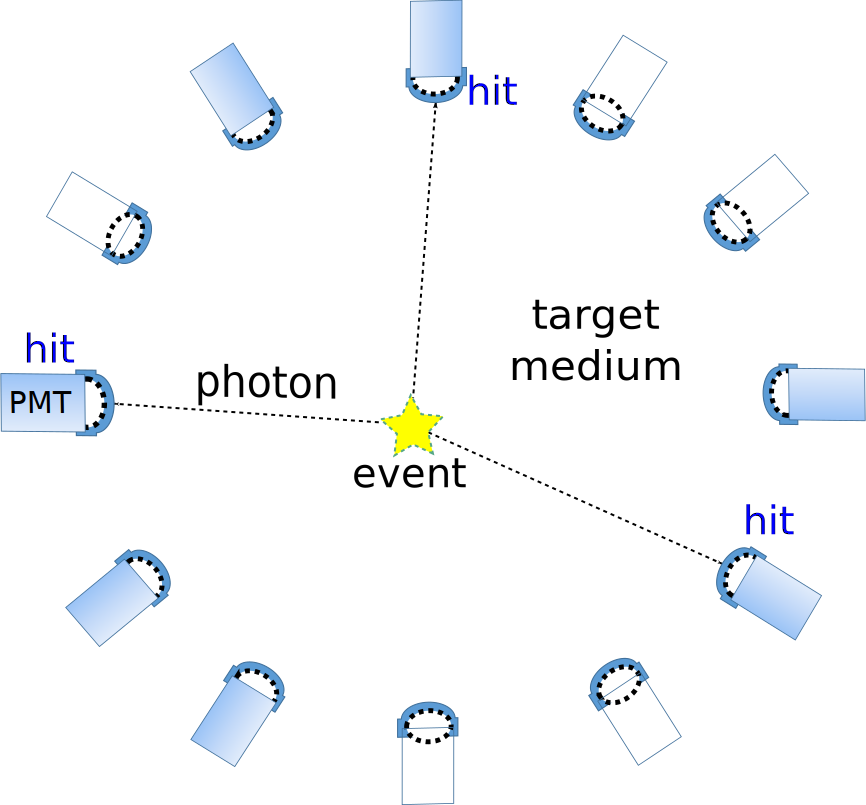
\includegraphics[width=\linewidth]{figures/detector.pdf}
  \caption{\label{fig:detector} Schematics of a typical PMT-based neutrino or dark matter detector.}
\end{subfigure}
\hfill
\begin{subfigure}{0.54\textwidth}
  \resizebox{\linewidth}{!}{%% Creator: Matplotlib, PGF backend
%%
%% To include the figure in your LaTeX document, write
%%   \input{<filename>.pgf}
%%
%% Make sure the required packages are loaded in your preamble
%%   \usepackage{pgf}
%%
%% and, on pdftex
%%   \usepackage[utf8]{inputenc}\DeclareUnicodeCharacter{2212}{-}
%%
%% or, on luatex and xetex
%%   \usepackage{unicode-math}
%%
%% Figures using additional raster images can only be included by \input if
%% they are in the same directory as the main LaTeX file. For loading figures
%% from other directories you can use the `import` package
%%   \usepackage{import}
%%
%% and then include the figures with
%%   \import{<path to file>}{<filename>.pgf}
%%
%% Matplotlib used the following preamble
%%
\begingroup%
\makeatletter%
\begin{pgfpicture}%
\pgfpathrectangle{\pgfpointorigin}{\pgfqpoint{8.000000in}{6.000000in}}%
\pgfusepath{use as bounding box, clip}%
\begin{pgfscope}%
\pgfsetbuttcap%
\pgfsetmiterjoin%
\definecolor{currentfill}{rgb}{1.000000,1.000000,1.000000}%
\pgfsetfillcolor{currentfill}%
\pgfsetlinewidth{0.000000pt}%
\definecolor{currentstroke}{rgb}{1.000000,1.000000,1.000000}%
\pgfsetstrokecolor{currentstroke}%
\pgfsetdash{}{0pt}%
\pgfpathmoveto{\pgfqpoint{0.000000in}{0.000000in}}%
\pgfpathlineto{\pgfqpoint{8.000000in}{0.000000in}}%
\pgfpathlineto{\pgfqpoint{8.000000in}{6.000000in}}%
\pgfpathlineto{\pgfqpoint{0.000000in}{6.000000in}}%
\pgfpathclose%
\pgfusepath{fill}%
\end{pgfscope}%
\begin{pgfscope}%
\pgfsetbuttcap%
\pgfsetmiterjoin%
\definecolor{currentfill}{rgb}{1.000000,1.000000,1.000000}%
\pgfsetfillcolor{currentfill}%
\pgfsetlinewidth{0.000000pt}%
\definecolor{currentstroke}{rgb}{0.000000,0.000000,0.000000}%
\pgfsetstrokecolor{currentstroke}%
\pgfsetstrokeopacity{0.000000}%
\pgfsetdash{}{0pt}%
\pgfpathmoveto{\pgfqpoint{1.200000in}{0.900000in}}%
\pgfpathlineto{\pgfqpoint{6.800000in}{0.900000in}}%
\pgfpathlineto{\pgfqpoint{6.800000in}{5.700000in}}%
\pgfpathlineto{\pgfqpoint{1.200000in}{5.700000in}}%
\pgfpathclose%
\pgfusepath{fill}%
\end{pgfscope}%
\begin{pgfscope}%
\pgfpathrectangle{\pgfqpoint{1.200000in}{0.900000in}}{\pgfqpoint{5.600000in}{4.800000in}}%
\pgfusepath{clip}%
\pgfsetrectcap%
\pgfsetroundjoin%
\pgfsetlinewidth{2.007500pt}%
\definecolor{currentstroke}{rgb}{0.000000,0.000000,1.000000}%
\pgfsetstrokecolor{currentstroke}%
\pgfsetdash{}{0pt}%
\pgfpathmoveto{\pgfqpoint{1.305660in}{1.883216in}}%
\pgfpathlineto{\pgfqpoint{1.326792in}{2.036248in}}%
\pgfpathlineto{\pgfqpoint{1.347925in}{2.202479in}}%
\pgfpathlineto{\pgfqpoint{1.379623in}{2.474750in}}%
\pgfpathlineto{\pgfqpoint{1.411321in}{2.770719in}}%
\pgfpathlineto{\pgfqpoint{1.453585in}{3.191895in}}%
\pgfpathlineto{\pgfqpoint{1.548679in}{4.159094in}}%
\pgfpathlineto{\pgfqpoint{1.580377in}{4.456532in}}%
\pgfpathlineto{\pgfqpoint{1.612075in}{4.727863in}}%
\pgfpathlineto{\pgfqpoint{1.633208in}{4.890990in}}%
\pgfpathlineto{\pgfqpoint{1.654340in}{5.038107in}}%
\pgfpathlineto{\pgfqpoint{1.675472in}{5.168088in}}%
\pgfpathlineto{\pgfqpoint{1.696604in}{5.280190in}}%
\pgfpathlineto{\pgfqpoint{1.717736in}{5.374061in}}%
\pgfpathlineto{\pgfqpoint{1.728302in}{5.414151in}}%
\pgfpathlineto{\pgfqpoint{1.738868in}{5.449716in}}%
\pgfpathlineto{\pgfqpoint{1.749434in}{5.480812in}}%
\pgfpathlineto{\pgfqpoint{1.760000in}{5.507512in}}%
\pgfpathlineto{\pgfqpoint{1.770566in}{5.529908in}}%
\pgfpathlineto{\pgfqpoint{1.781132in}{5.548108in}}%
\pgfpathlineto{\pgfqpoint{1.791698in}{5.562234in}}%
\pgfpathlineto{\pgfqpoint{1.802264in}{5.572421in}}%
\pgfpathlineto{\pgfqpoint{1.812830in}{5.578813in}}%
\pgfpathlineto{\pgfqpoint{1.823396in}{5.581568in}}%
\pgfpathlineto{\pgfqpoint{1.833962in}{5.580847in}}%
\pgfpathlineto{\pgfqpoint{1.844528in}{5.576820in}}%
\pgfpathlineto{\pgfqpoint{1.855094in}{5.569661in}}%
\pgfpathlineto{\pgfqpoint{1.865660in}{5.559546in}}%
\pgfpathlineto{\pgfqpoint{1.876226in}{5.546654in}}%
\pgfpathlineto{\pgfqpoint{1.886792in}{5.531163in}}%
\pgfpathlineto{\pgfqpoint{1.897358in}{5.513251in}}%
\pgfpathlineto{\pgfqpoint{1.918491in}{5.470862in}}%
\pgfpathlineto{\pgfqpoint{1.939623in}{5.420846in}}%
\pgfpathlineto{\pgfqpoint{1.960755in}{5.364485in}}%
\pgfpathlineto{\pgfqpoint{1.992453in}{5.270608in}}%
\pgfpathlineto{\pgfqpoint{2.024151in}{5.168617in}}%
\pgfpathlineto{\pgfqpoint{2.066415in}{5.024973in}}%
\pgfpathlineto{\pgfqpoint{2.235472in}{4.441688in}}%
\pgfpathlineto{\pgfqpoint{2.288302in}{4.270330in}}%
\pgfpathlineto{\pgfqpoint{2.341132in}{4.106510in}}%
\pgfpathlineto{\pgfqpoint{2.393962in}{3.950336in}}%
\pgfpathlineto{\pgfqpoint{2.446792in}{3.801644in}}%
\pgfpathlineto{\pgfqpoint{2.499623in}{3.660154in}}%
\pgfpathlineto{\pgfqpoint{2.552453in}{3.525548in}}%
\pgfpathlineto{\pgfqpoint{2.605283in}{3.397501in}}%
\pgfpathlineto{\pgfqpoint{2.658113in}{3.275697in}}%
\pgfpathlineto{\pgfqpoint{2.710943in}{3.159833in}}%
\pgfpathlineto{\pgfqpoint{2.763774in}{3.049620in}}%
\pgfpathlineto{\pgfqpoint{2.816604in}{2.944781in}}%
\pgfpathlineto{\pgfqpoint{2.869434in}{2.845056in}}%
\pgfpathlineto{\pgfqpoint{2.922264in}{2.750195in}}%
\pgfpathlineto{\pgfqpoint{2.975094in}{2.659960in}}%
\pgfpathlineto{\pgfqpoint{3.027925in}{2.574125in}}%
\pgfpathlineto{\pgfqpoint{3.080755in}{2.492477in}}%
\pgfpathlineto{\pgfqpoint{3.133585in}{2.414811in}}%
\pgfpathlineto{\pgfqpoint{3.186415in}{2.340933in}}%
\pgfpathlineto{\pgfqpoint{3.239245in}{2.270658in}}%
\pgfpathlineto{\pgfqpoint{3.292075in}{2.203810in}}%
\pgfpathlineto{\pgfqpoint{3.344906in}{2.140223in}}%
\pgfpathlineto{\pgfqpoint{3.397736in}{2.079736in}}%
\pgfpathlineto{\pgfqpoint{3.450566in}{2.022200in}}%
\pgfpathlineto{\pgfqpoint{3.503396in}{1.967469in}}%
\pgfpathlineto{\pgfqpoint{3.566792in}{1.905305in}}%
\pgfpathlineto{\pgfqpoint{3.630189in}{1.846760in}}%
\pgfpathlineto{\pgfqpoint{3.693585in}{1.791625in}}%
\pgfpathlineto{\pgfqpoint{3.756981in}{1.739701in}}%
\pgfpathlineto{\pgfqpoint{3.820377in}{1.690801in}}%
\pgfpathlineto{\pgfqpoint{3.883774in}{1.644748in}}%
\pgfpathlineto{\pgfqpoint{3.947170in}{1.601377in}}%
\pgfpathlineto{\pgfqpoint{4.010566in}{1.560532in}}%
\pgfpathlineto{\pgfqpoint{4.073962in}{1.522066in}}%
\pgfpathlineto{\pgfqpoint{4.147925in}{1.480010in}}%
\pgfpathlineto{\pgfqpoint{4.221887in}{1.440798in}}%
\pgfpathlineto{\pgfqpoint{4.295849in}{1.404237in}}%
\pgfpathlineto{\pgfqpoint{4.369811in}{1.370147in}}%
\pgfpathlineto{\pgfqpoint{4.443774in}{1.338362in}}%
\pgfpathlineto{\pgfqpoint{4.528302in}{1.304660in}}%
\pgfpathlineto{\pgfqpoint{4.612830in}{1.273548in}}%
\pgfpathlineto{\pgfqpoint{4.697358in}{1.244828in}}%
\pgfpathlineto{\pgfqpoint{4.781887in}{1.218316in}}%
\pgfpathlineto{\pgfqpoint{4.876981in}{1.190919in}}%
\pgfpathlineto{\pgfqpoint{4.972075in}{1.165880in}}%
\pgfpathlineto{\pgfqpoint{5.067170in}{1.142996in}}%
\pgfpathlineto{\pgfqpoint{5.172830in}{1.119872in}}%
\pgfpathlineto{\pgfqpoint{5.278491in}{1.098949in}}%
\pgfpathlineto{\pgfqpoint{5.394717in}{1.078225in}}%
\pgfpathlineto{\pgfqpoint{5.510943in}{1.059660in}}%
\pgfpathlineto{\pgfqpoint{5.637736in}{1.041606in}}%
\pgfpathlineto{\pgfqpoint{5.775094in}{1.024343in}}%
\pgfpathlineto{\pgfqpoint{5.923019in}{1.008099in}}%
\pgfpathlineto{\pgfqpoint{6.081509in}{0.993042in}}%
\pgfpathlineto{\pgfqpoint{6.250566in}{0.979285in}}%
\pgfpathlineto{\pgfqpoint{6.430189in}{0.966890in}}%
\pgfpathlineto{\pgfqpoint{6.630943in}{0.955315in}}%
\pgfpathlineto{\pgfqpoint{6.789434in}{0.947610in}}%
\pgfpathlineto{\pgfqpoint{6.789434in}{0.947610in}}%
\pgfusepath{stroke}%
\end{pgfscope}%
\begin{pgfscope}%
\pgfsetrectcap%
\pgfsetmiterjoin%
\pgfsetlinewidth{1.003750pt}%
\definecolor{currentstroke}{rgb}{0.000000,0.000000,0.000000}%
\pgfsetstrokecolor{currentstroke}%
\pgfsetdash{}{0pt}%
\pgfpathmoveto{\pgfqpoint{1.200000in}{0.900000in}}%
\pgfpathlineto{\pgfqpoint{1.200000in}{5.700000in}}%
\pgfusepath{stroke}%
\end{pgfscope}%
\begin{pgfscope}%
\pgfsetrectcap%
\pgfsetmiterjoin%
\pgfsetlinewidth{1.003750pt}%
\definecolor{currentstroke}{rgb}{0.000000,0.000000,0.000000}%
\pgfsetstrokecolor{currentstroke}%
\pgfsetdash{}{0pt}%
\pgfpathmoveto{\pgfqpoint{6.800000in}{0.900000in}}%
\pgfpathlineto{\pgfqpoint{6.800000in}{5.700000in}}%
\pgfusepath{stroke}%
\end{pgfscope}%
\begin{pgfscope}%
\pgfsetrectcap%
\pgfsetmiterjoin%
\pgfsetlinewidth{1.003750pt}%
\definecolor{currentstroke}{rgb}{0.000000,0.000000,0.000000}%
\pgfsetstrokecolor{currentstroke}%
\pgfsetdash{}{0pt}%
\pgfpathmoveto{\pgfqpoint{1.200000in}{0.900000in}}%
\pgfpathlineto{\pgfqpoint{6.800000in}{0.900000in}}%
\pgfusepath{stroke}%
\end{pgfscope}%
\begin{pgfscope}%
\pgfsetrectcap%
\pgfsetmiterjoin%
\pgfsetlinewidth{1.003750pt}%
\definecolor{currentstroke}{rgb}{0.000000,0.000000,0.000000}%
\pgfsetstrokecolor{currentstroke}%
\pgfsetdash{}{0pt}%
\pgfpathmoveto{\pgfqpoint{1.200000in}{5.700000in}}%
\pgfpathlineto{\pgfqpoint{6.800000in}{5.700000in}}%
\pgfusepath{stroke}%
\end{pgfscope}%
\begin{pgfscope}%
\pgfpathrectangle{\pgfqpoint{1.200000in}{0.900000in}}{\pgfqpoint{5.600000in}{4.800000in}}%
\pgfusepath{clip}%
\pgfsetbuttcap%
\pgfsetroundjoin%
\pgfsetlinewidth{0.501875pt}%
\definecolor{currentstroke}{rgb}{0.000000,0.000000,0.000000}%
\pgfsetstrokecolor{currentstroke}%
\pgfsetdash{{1.000000pt}{3.000000pt}}{0.000000pt}%
\pgfpathmoveto{\pgfqpoint{1.516981in}{0.900000in}}%
\pgfpathlineto{\pgfqpoint{1.516981in}{5.700000in}}%
\pgfusepath{stroke}%
\end{pgfscope}%
\begin{pgfscope}%
\pgfsetbuttcap%
\pgfsetroundjoin%
\definecolor{currentfill}{rgb}{0.000000,0.000000,0.000000}%
\pgfsetfillcolor{currentfill}%
\pgfsetlinewidth{0.501875pt}%
\definecolor{currentstroke}{rgb}{0.000000,0.000000,0.000000}%
\pgfsetstrokecolor{currentstroke}%
\pgfsetdash{}{0pt}%
\pgfsys@defobject{currentmarker}{\pgfqpoint{0.000000in}{0.000000in}}{\pgfqpoint{0.000000in}{0.055556in}}{%
\pgfpathmoveto{\pgfqpoint{0.000000in}{0.000000in}}%
\pgfpathlineto{\pgfqpoint{0.000000in}{0.055556in}}%
\pgfusepath{stroke,fill}%
}%
\begin{pgfscope}%
\pgfsys@transformshift{1.516981in}{0.900000in}%
\pgfsys@useobject{currentmarker}{}%
\end{pgfscope}%
\end{pgfscope}%
\begin{pgfscope}%
\pgfsetbuttcap%
\pgfsetroundjoin%
\definecolor{currentfill}{rgb}{0.000000,0.000000,0.000000}%
\pgfsetfillcolor{currentfill}%
\pgfsetlinewidth{0.501875pt}%
\definecolor{currentstroke}{rgb}{0.000000,0.000000,0.000000}%
\pgfsetstrokecolor{currentstroke}%
\pgfsetdash{}{0pt}%
\pgfsys@defobject{currentmarker}{\pgfqpoint{0.000000in}{-0.055556in}}{\pgfqpoint{0.000000in}{0.000000in}}{%
\pgfpathmoveto{\pgfqpoint{0.000000in}{0.000000in}}%
\pgfpathlineto{\pgfqpoint{0.000000in}{-0.055556in}}%
\pgfusepath{stroke,fill}%
}%
\begin{pgfscope}%
\pgfsys@transformshift{1.516981in}{5.700000in}%
\pgfsys@useobject{currentmarker}{}%
\end{pgfscope}%
\end{pgfscope}%
\begin{pgfscope}%
\definecolor{textcolor}{rgb}{0.000000,0.000000,0.000000}%
\pgfsetstrokecolor{textcolor}%
\pgfsetfillcolor{textcolor}%
\pgftext[x=1.516981in,y=0.844444in,,top]{\color{textcolor}\sffamily\fontsize{20.000000}{24.000000}\selectfont \(\displaystyle {0}\)}%
\end{pgfscope}%
\begin{pgfscope}%
\pgfpathrectangle{\pgfqpoint{1.200000in}{0.900000in}}{\pgfqpoint{5.600000in}{4.800000in}}%
\pgfusepath{clip}%
\pgfsetbuttcap%
\pgfsetroundjoin%
\pgfsetlinewidth{0.501875pt}%
\definecolor{currentstroke}{rgb}{0.000000,0.000000,0.000000}%
\pgfsetstrokecolor{currentstroke}%
\pgfsetdash{{1.000000pt}{3.000000pt}}{0.000000pt}%
\pgfpathmoveto{\pgfqpoint{2.573585in}{0.900000in}}%
\pgfpathlineto{\pgfqpoint{2.573585in}{5.700000in}}%
\pgfusepath{stroke}%
\end{pgfscope}%
\begin{pgfscope}%
\pgfsetbuttcap%
\pgfsetroundjoin%
\definecolor{currentfill}{rgb}{0.000000,0.000000,0.000000}%
\pgfsetfillcolor{currentfill}%
\pgfsetlinewidth{0.501875pt}%
\definecolor{currentstroke}{rgb}{0.000000,0.000000,0.000000}%
\pgfsetstrokecolor{currentstroke}%
\pgfsetdash{}{0pt}%
\pgfsys@defobject{currentmarker}{\pgfqpoint{0.000000in}{0.000000in}}{\pgfqpoint{0.000000in}{0.055556in}}{%
\pgfpathmoveto{\pgfqpoint{0.000000in}{0.000000in}}%
\pgfpathlineto{\pgfqpoint{0.000000in}{0.055556in}}%
\pgfusepath{stroke,fill}%
}%
\begin{pgfscope}%
\pgfsys@transformshift{2.573585in}{0.900000in}%
\pgfsys@useobject{currentmarker}{}%
\end{pgfscope}%
\end{pgfscope}%
\begin{pgfscope}%
\pgfsetbuttcap%
\pgfsetroundjoin%
\definecolor{currentfill}{rgb}{0.000000,0.000000,0.000000}%
\pgfsetfillcolor{currentfill}%
\pgfsetlinewidth{0.501875pt}%
\definecolor{currentstroke}{rgb}{0.000000,0.000000,0.000000}%
\pgfsetstrokecolor{currentstroke}%
\pgfsetdash{}{0pt}%
\pgfsys@defobject{currentmarker}{\pgfqpoint{0.000000in}{-0.055556in}}{\pgfqpoint{0.000000in}{0.000000in}}{%
\pgfpathmoveto{\pgfqpoint{0.000000in}{0.000000in}}%
\pgfpathlineto{\pgfqpoint{0.000000in}{-0.055556in}}%
\pgfusepath{stroke,fill}%
}%
\begin{pgfscope}%
\pgfsys@transformshift{2.573585in}{5.700000in}%
\pgfsys@useobject{currentmarker}{}%
\end{pgfscope}%
\end{pgfscope}%
\begin{pgfscope}%
\definecolor{textcolor}{rgb}{0.000000,0.000000,0.000000}%
\pgfsetstrokecolor{textcolor}%
\pgfsetfillcolor{textcolor}%
\pgftext[x=2.573585in,y=0.844444in,,top]{\color{textcolor}\sffamily\fontsize{20.000000}{24.000000}\selectfont \(\displaystyle {10}\)}%
\end{pgfscope}%
\begin{pgfscope}%
\pgfpathrectangle{\pgfqpoint{1.200000in}{0.900000in}}{\pgfqpoint{5.600000in}{4.800000in}}%
\pgfusepath{clip}%
\pgfsetbuttcap%
\pgfsetroundjoin%
\pgfsetlinewidth{0.501875pt}%
\definecolor{currentstroke}{rgb}{0.000000,0.000000,0.000000}%
\pgfsetstrokecolor{currentstroke}%
\pgfsetdash{{1.000000pt}{3.000000pt}}{0.000000pt}%
\pgfpathmoveto{\pgfqpoint{3.630189in}{0.900000in}}%
\pgfpathlineto{\pgfqpoint{3.630189in}{5.700000in}}%
\pgfusepath{stroke}%
\end{pgfscope}%
\begin{pgfscope}%
\pgfsetbuttcap%
\pgfsetroundjoin%
\definecolor{currentfill}{rgb}{0.000000,0.000000,0.000000}%
\pgfsetfillcolor{currentfill}%
\pgfsetlinewidth{0.501875pt}%
\definecolor{currentstroke}{rgb}{0.000000,0.000000,0.000000}%
\pgfsetstrokecolor{currentstroke}%
\pgfsetdash{}{0pt}%
\pgfsys@defobject{currentmarker}{\pgfqpoint{0.000000in}{0.000000in}}{\pgfqpoint{0.000000in}{0.055556in}}{%
\pgfpathmoveto{\pgfqpoint{0.000000in}{0.000000in}}%
\pgfpathlineto{\pgfqpoint{0.000000in}{0.055556in}}%
\pgfusepath{stroke,fill}%
}%
\begin{pgfscope}%
\pgfsys@transformshift{3.630189in}{0.900000in}%
\pgfsys@useobject{currentmarker}{}%
\end{pgfscope}%
\end{pgfscope}%
\begin{pgfscope}%
\pgfsetbuttcap%
\pgfsetroundjoin%
\definecolor{currentfill}{rgb}{0.000000,0.000000,0.000000}%
\pgfsetfillcolor{currentfill}%
\pgfsetlinewidth{0.501875pt}%
\definecolor{currentstroke}{rgb}{0.000000,0.000000,0.000000}%
\pgfsetstrokecolor{currentstroke}%
\pgfsetdash{}{0pt}%
\pgfsys@defobject{currentmarker}{\pgfqpoint{0.000000in}{-0.055556in}}{\pgfqpoint{0.000000in}{0.000000in}}{%
\pgfpathmoveto{\pgfqpoint{0.000000in}{0.000000in}}%
\pgfpathlineto{\pgfqpoint{0.000000in}{-0.055556in}}%
\pgfusepath{stroke,fill}%
}%
\begin{pgfscope}%
\pgfsys@transformshift{3.630189in}{5.700000in}%
\pgfsys@useobject{currentmarker}{}%
\end{pgfscope}%
\end{pgfscope}%
\begin{pgfscope}%
\definecolor{textcolor}{rgb}{0.000000,0.000000,0.000000}%
\pgfsetstrokecolor{textcolor}%
\pgfsetfillcolor{textcolor}%
\pgftext[x=3.630189in,y=0.844444in,,top]{\color{textcolor}\sffamily\fontsize{20.000000}{24.000000}\selectfont \(\displaystyle {20}\)}%
\end{pgfscope}%
\begin{pgfscope}%
\pgfpathrectangle{\pgfqpoint{1.200000in}{0.900000in}}{\pgfqpoint{5.600000in}{4.800000in}}%
\pgfusepath{clip}%
\pgfsetbuttcap%
\pgfsetroundjoin%
\pgfsetlinewidth{0.501875pt}%
\definecolor{currentstroke}{rgb}{0.000000,0.000000,0.000000}%
\pgfsetstrokecolor{currentstroke}%
\pgfsetdash{{1.000000pt}{3.000000pt}}{0.000000pt}%
\pgfpathmoveto{\pgfqpoint{4.686792in}{0.900000in}}%
\pgfpathlineto{\pgfqpoint{4.686792in}{5.700000in}}%
\pgfusepath{stroke}%
\end{pgfscope}%
\begin{pgfscope}%
\pgfsetbuttcap%
\pgfsetroundjoin%
\definecolor{currentfill}{rgb}{0.000000,0.000000,0.000000}%
\pgfsetfillcolor{currentfill}%
\pgfsetlinewidth{0.501875pt}%
\definecolor{currentstroke}{rgb}{0.000000,0.000000,0.000000}%
\pgfsetstrokecolor{currentstroke}%
\pgfsetdash{}{0pt}%
\pgfsys@defobject{currentmarker}{\pgfqpoint{0.000000in}{0.000000in}}{\pgfqpoint{0.000000in}{0.055556in}}{%
\pgfpathmoveto{\pgfqpoint{0.000000in}{0.000000in}}%
\pgfpathlineto{\pgfqpoint{0.000000in}{0.055556in}}%
\pgfusepath{stroke,fill}%
}%
\begin{pgfscope}%
\pgfsys@transformshift{4.686792in}{0.900000in}%
\pgfsys@useobject{currentmarker}{}%
\end{pgfscope}%
\end{pgfscope}%
\begin{pgfscope}%
\pgfsetbuttcap%
\pgfsetroundjoin%
\definecolor{currentfill}{rgb}{0.000000,0.000000,0.000000}%
\pgfsetfillcolor{currentfill}%
\pgfsetlinewidth{0.501875pt}%
\definecolor{currentstroke}{rgb}{0.000000,0.000000,0.000000}%
\pgfsetstrokecolor{currentstroke}%
\pgfsetdash{}{0pt}%
\pgfsys@defobject{currentmarker}{\pgfqpoint{0.000000in}{-0.055556in}}{\pgfqpoint{0.000000in}{0.000000in}}{%
\pgfpathmoveto{\pgfqpoint{0.000000in}{0.000000in}}%
\pgfpathlineto{\pgfqpoint{0.000000in}{-0.055556in}}%
\pgfusepath{stroke,fill}%
}%
\begin{pgfscope}%
\pgfsys@transformshift{4.686792in}{5.700000in}%
\pgfsys@useobject{currentmarker}{}%
\end{pgfscope}%
\end{pgfscope}%
\begin{pgfscope}%
\definecolor{textcolor}{rgb}{0.000000,0.000000,0.000000}%
\pgfsetstrokecolor{textcolor}%
\pgfsetfillcolor{textcolor}%
\pgftext[x=4.686792in,y=0.844444in,,top]{\color{textcolor}\sffamily\fontsize{20.000000}{24.000000}\selectfont \(\displaystyle {30}\)}%
\end{pgfscope}%
\begin{pgfscope}%
\pgfpathrectangle{\pgfqpoint{1.200000in}{0.900000in}}{\pgfqpoint{5.600000in}{4.800000in}}%
\pgfusepath{clip}%
\pgfsetbuttcap%
\pgfsetroundjoin%
\pgfsetlinewidth{0.501875pt}%
\definecolor{currentstroke}{rgb}{0.000000,0.000000,0.000000}%
\pgfsetstrokecolor{currentstroke}%
\pgfsetdash{{1.000000pt}{3.000000pt}}{0.000000pt}%
\pgfpathmoveto{\pgfqpoint{5.743396in}{0.900000in}}%
\pgfpathlineto{\pgfqpoint{5.743396in}{5.700000in}}%
\pgfusepath{stroke}%
\end{pgfscope}%
\begin{pgfscope}%
\pgfsetbuttcap%
\pgfsetroundjoin%
\definecolor{currentfill}{rgb}{0.000000,0.000000,0.000000}%
\pgfsetfillcolor{currentfill}%
\pgfsetlinewidth{0.501875pt}%
\definecolor{currentstroke}{rgb}{0.000000,0.000000,0.000000}%
\pgfsetstrokecolor{currentstroke}%
\pgfsetdash{}{0pt}%
\pgfsys@defobject{currentmarker}{\pgfqpoint{0.000000in}{0.000000in}}{\pgfqpoint{0.000000in}{0.055556in}}{%
\pgfpathmoveto{\pgfqpoint{0.000000in}{0.000000in}}%
\pgfpathlineto{\pgfqpoint{0.000000in}{0.055556in}}%
\pgfusepath{stroke,fill}%
}%
\begin{pgfscope}%
\pgfsys@transformshift{5.743396in}{0.900000in}%
\pgfsys@useobject{currentmarker}{}%
\end{pgfscope}%
\end{pgfscope}%
\begin{pgfscope}%
\pgfsetbuttcap%
\pgfsetroundjoin%
\definecolor{currentfill}{rgb}{0.000000,0.000000,0.000000}%
\pgfsetfillcolor{currentfill}%
\pgfsetlinewidth{0.501875pt}%
\definecolor{currentstroke}{rgb}{0.000000,0.000000,0.000000}%
\pgfsetstrokecolor{currentstroke}%
\pgfsetdash{}{0pt}%
\pgfsys@defobject{currentmarker}{\pgfqpoint{0.000000in}{-0.055556in}}{\pgfqpoint{0.000000in}{0.000000in}}{%
\pgfpathmoveto{\pgfqpoint{0.000000in}{0.000000in}}%
\pgfpathlineto{\pgfqpoint{0.000000in}{-0.055556in}}%
\pgfusepath{stroke,fill}%
}%
\begin{pgfscope}%
\pgfsys@transformshift{5.743396in}{5.700000in}%
\pgfsys@useobject{currentmarker}{}%
\end{pgfscope}%
\end{pgfscope}%
\begin{pgfscope}%
\definecolor{textcolor}{rgb}{0.000000,0.000000,0.000000}%
\pgfsetstrokecolor{textcolor}%
\pgfsetfillcolor{textcolor}%
\pgftext[x=5.743396in,y=0.844444in,,top]{\color{textcolor}\sffamily\fontsize{20.000000}{24.000000}\selectfont \(\displaystyle {40}\)}%
\end{pgfscope}%
\begin{pgfscope}%
\pgfpathrectangle{\pgfqpoint{1.200000in}{0.900000in}}{\pgfqpoint{5.600000in}{4.800000in}}%
\pgfusepath{clip}%
\pgfsetbuttcap%
\pgfsetroundjoin%
\pgfsetlinewidth{0.501875pt}%
\definecolor{currentstroke}{rgb}{0.000000,0.000000,0.000000}%
\pgfsetstrokecolor{currentstroke}%
\pgfsetdash{{1.000000pt}{3.000000pt}}{0.000000pt}%
\pgfpathmoveto{\pgfqpoint{6.800000in}{0.900000in}}%
\pgfpathlineto{\pgfqpoint{6.800000in}{5.700000in}}%
\pgfusepath{stroke}%
\end{pgfscope}%
\begin{pgfscope}%
\pgfsetbuttcap%
\pgfsetroundjoin%
\definecolor{currentfill}{rgb}{0.000000,0.000000,0.000000}%
\pgfsetfillcolor{currentfill}%
\pgfsetlinewidth{0.501875pt}%
\definecolor{currentstroke}{rgb}{0.000000,0.000000,0.000000}%
\pgfsetstrokecolor{currentstroke}%
\pgfsetdash{}{0pt}%
\pgfsys@defobject{currentmarker}{\pgfqpoint{0.000000in}{0.000000in}}{\pgfqpoint{0.000000in}{0.055556in}}{%
\pgfpathmoveto{\pgfqpoint{0.000000in}{0.000000in}}%
\pgfpathlineto{\pgfqpoint{0.000000in}{0.055556in}}%
\pgfusepath{stroke,fill}%
}%
\begin{pgfscope}%
\pgfsys@transformshift{6.800000in}{0.900000in}%
\pgfsys@useobject{currentmarker}{}%
\end{pgfscope}%
\end{pgfscope}%
\begin{pgfscope}%
\pgfsetbuttcap%
\pgfsetroundjoin%
\definecolor{currentfill}{rgb}{0.000000,0.000000,0.000000}%
\pgfsetfillcolor{currentfill}%
\pgfsetlinewidth{0.501875pt}%
\definecolor{currentstroke}{rgb}{0.000000,0.000000,0.000000}%
\pgfsetstrokecolor{currentstroke}%
\pgfsetdash{}{0pt}%
\pgfsys@defobject{currentmarker}{\pgfqpoint{0.000000in}{-0.055556in}}{\pgfqpoint{0.000000in}{0.000000in}}{%
\pgfpathmoveto{\pgfqpoint{0.000000in}{0.000000in}}%
\pgfpathlineto{\pgfqpoint{0.000000in}{-0.055556in}}%
\pgfusepath{stroke,fill}%
}%
\begin{pgfscope}%
\pgfsys@transformshift{6.800000in}{5.700000in}%
\pgfsys@useobject{currentmarker}{}%
\end{pgfscope}%
\end{pgfscope}%
\begin{pgfscope}%
\definecolor{textcolor}{rgb}{0.000000,0.000000,0.000000}%
\pgfsetstrokecolor{textcolor}%
\pgfsetfillcolor{textcolor}%
\pgftext[x=6.800000in,y=0.844444in,,top]{\color{textcolor}\sffamily\fontsize{20.000000}{24.000000}\selectfont \(\displaystyle {50}\)}%
\end{pgfscope}%
\begin{pgfscope}%
\definecolor{textcolor}{rgb}{0.000000,0.000000,0.000000}%
\pgfsetstrokecolor{textcolor}%
\pgfsetfillcolor{textcolor}%
\pgftext[x=4.000000in,y=0.518932in,,top]{\color{textcolor}\sffamily\fontsize{20.000000}{24.000000}\selectfont \(\displaystyle t/\mathrm{ns}\)}%
\end{pgfscope}%
\begin{pgfscope}%
\pgfpathrectangle{\pgfqpoint{1.200000in}{0.900000in}}{\pgfqpoint{5.600000in}{4.800000in}}%
\pgfusepath{clip}%
\pgfsetbuttcap%
\pgfsetroundjoin%
\pgfsetlinewidth{0.501875pt}%
\definecolor{currentstroke}{rgb}{0.000000,0.000000,0.000000}%
\pgfsetstrokecolor{currentstroke}%
\pgfsetdash{{1.000000pt}{3.000000pt}}{0.000000pt}%
\pgfpathmoveto{\pgfqpoint{1.200000in}{0.900000in}}%
\pgfpathlineto{\pgfqpoint{6.800000in}{0.900000in}}%
\pgfusepath{stroke}%
\end{pgfscope}%
\begin{pgfscope}%
\pgfsetbuttcap%
\pgfsetroundjoin%
\definecolor{currentfill}{rgb}{0.000000,0.000000,0.000000}%
\pgfsetfillcolor{currentfill}%
\pgfsetlinewidth{0.501875pt}%
\definecolor{currentstroke}{rgb}{0.000000,0.000000,0.000000}%
\pgfsetstrokecolor{currentstroke}%
\pgfsetdash{}{0pt}%
\pgfsys@defobject{currentmarker}{\pgfqpoint{0.000000in}{0.000000in}}{\pgfqpoint{0.055556in}{0.000000in}}{%
\pgfpathmoveto{\pgfqpoint{0.000000in}{0.000000in}}%
\pgfpathlineto{\pgfqpoint{0.055556in}{0.000000in}}%
\pgfusepath{stroke,fill}%
}%
\begin{pgfscope}%
\pgfsys@transformshift{1.200000in}{0.900000in}%
\pgfsys@useobject{currentmarker}{}%
\end{pgfscope}%
\end{pgfscope}%
\begin{pgfscope}%
\pgfsetbuttcap%
\pgfsetroundjoin%
\definecolor{currentfill}{rgb}{0.000000,0.000000,0.000000}%
\pgfsetfillcolor{currentfill}%
\pgfsetlinewidth{0.501875pt}%
\definecolor{currentstroke}{rgb}{0.000000,0.000000,0.000000}%
\pgfsetstrokecolor{currentstroke}%
\pgfsetdash{}{0pt}%
\pgfsys@defobject{currentmarker}{\pgfqpoint{-0.055556in}{0.000000in}}{\pgfqpoint{0.000000in}{0.000000in}}{%
\pgfpathmoveto{\pgfqpoint{0.000000in}{0.000000in}}%
\pgfpathlineto{\pgfqpoint{-0.055556in}{0.000000in}}%
\pgfusepath{stroke,fill}%
}%
\begin{pgfscope}%
\pgfsys@transformshift{6.800000in}{0.900000in}%
\pgfsys@useobject{currentmarker}{}%
\end{pgfscope}%
\end{pgfscope}%
\begin{pgfscope}%
\definecolor{textcolor}{rgb}{0.000000,0.000000,0.000000}%
\pgfsetstrokecolor{textcolor}%
\pgfsetfillcolor{textcolor}%
\pgftext[x=1.144444in,y=0.900000in,right,]{\color{textcolor}\sffamily\fontsize{20.000000}{24.000000}\selectfont \(\displaystyle {0.00}\)}%
\end{pgfscope}%
\begin{pgfscope}%
\pgfpathrectangle{\pgfqpoint{1.200000in}{0.900000in}}{\pgfqpoint{5.600000in}{4.800000in}}%
\pgfusepath{clip}%
\pgfsetbuttcap%
\pgfsetroundjoin%
\pgfsetlinewidth{0.501875pt}%
\definecolor{currentstroke}{rgb}{0.000000,0.000000,0.000000}%
\pgfsetstrokecolor{currentstroke}%
\pgfsetdash{{1.000000pt}{3.000000pt}}{0.000000pt}%
\pgfpathmoveto{\pgfqpoint{1.200000in}{1.585714in}}%
\pgfpathlineto{\pgfqpoint{6.800000in}{1.585714in}}%
\pgfusepath{stroke}%
\end{pgfscope}%
\begin{pgfscope}%
\pgfsetbuttcap%
\pgfsetroundjoin%
\definecolor{currentfill}{rgb}{0.000000,0.000000,0.000000}%
\pgfsetfillcolor{currentfill}%
\pgfsetlinewidth{0.501875pt}%
\definecolor{currentstroke}{rgb}{0.000000,0.000000,0.000000}%
\pgfsetstrokecolor{currentstroke}%
\pgfsetdash{}{0pt}%
\pgfsys@defobject{currentmarker}{\pgfqpoint{0.000000in}{0.000000in}}{\pgfqpoint{0.055556in}{0.000000in}}{%
\pgfpathmoveto{\pgfqpoint{0.000000in}{0.000000in}}%
\pgfpathlineto{\pgfqpoint{0.055556in}{0.000000in}}%
\pgfusepath{stroke,fill}%
}%
\begin{pgfscope}%
\pgfsys@transformshift{1.200000in}{1.585714in}%
\pgfsys@useobject{currentmarker}{}%
\end{pgfscope}%
\end{pgfscope}%
\begin{pgfscope}%
\pgfsetbuttcap%
\pgfsetroundjoin%
\definecolor{currentfill}{rgb}{0.000000,0.000000,0.000000}%
\pgfsetfillcolor{currentfill}%
\pgfsetlinewidth{0.501875pt}%
\definecolor{currentstroke}{rgb}{0.000000,0.000000,0.000000}%
\pgfsetstrokecolor{currentstroke}%
\pgfsetdash{}{0pt}%
\pgfsys@defobject{currentmarker}{\pgfqpoint{-0.055556in}{0.000000in}}{\pgfqpoint{0.000000in}{0.000000in}}{%
\pgfpathmoveto{\pgfqpoint{0.000000in}{0.000000in}}%
\pgfpathlineto{\pgfqpoint{-0.055556in}{0.000000in}}%
\pgfusepath{stroke,fill}%
}%
\begin{pgfscope}%
\pgfsys@transformshift{6.800000in}{1.585714in}%
\pgfsys@useobject{currentmarker}{}%
\end{pgfscope}%
\end{pgfscope}%
\begin{pgfscope}%
\definecolor{textcolor}{rgb}{0.000000,0.000000,0.000000}%
\pgfsetstrokecolor{textcolor}%
\pgfsetfillcolor{textcolor}%
\pgftext[x=1.144444in,y=1.585714in,right,]{\color{textcolor}\sffamily\fontsize{20.000000}{24.000000}\selectfont \(\displaystyle {0.01}\)}%
\end{pgfscope}%
\begin{pgfscope}%
\pgfpathrectangle{\pgfqpoint{1.200000in}{0.900000in}}{\pgfqpoint{5.600000in}{4.800000in}}%
\pgfusepath{clip}%
\pgfsetbuttcap%
\pgfsetroundjoin%
\pgfsetlinewidth{0.501875pt}%
\definecolor{currentstroke}{rgb}{0.000000,0.000000,0.000000}%
\pgfsetstrokecolor{currentstroke}%
\pgfsetdash{{1.000000pt}{3.000000pt}}{0.000000pt}%
\pgfpathmoveto{\pgfqpoint{1.200000in}{2.271429in}}%
\pgfpathlineto{\pgfqpoint{6.800000in}{2.271429in}}%
\pgfusepath{stroke}%
\end{pgfscope}%
\begin{pgfscope}%
\pgfsetbuttcap%
\pgfsetroundjoin%
\definecolor{currentfill}{rgb}{0.000000,0.000000,0.000000}%
\pgfsetfillcolor{currentfill}%
\pgfsetlinewidth{0.501875pt}%
\definecolor{currentstroke}{rgb}{0.000000,0.000000,0.000000}%
\pgfsetstrokecolor{currentstroke}%
\pgfsetdash{}{0pt}%
\pgfsys@defobject{currentmarker}{\pgfqpoint{0.000000in}{0.000000in}}{\pgfqpoint{0.055556in}{0.000000in}}{%
\pgfpathmoveto{\pgfqpoint{0.000000in}{0.000000in}}%
\pgfpathlineto{\pgfqpoint{0.055556in}{0.000000in}}%
\pgfusepath{stroke,fill}%
}%
\begin{pgfscope}%
\pgfsys@transformshift{1.200000in}{2.271429in}%
\pgfsys@useobject{currentmarker}{}%
\end{pgfscope}%
\end{pgfscope}%
\begin{pgfscope}%
\pgfsetbuttcap%
\pgfsetroundjoin%
\definecolor{currentfill}{rgb}{0.000000,0.000000,0.000000}%
\pgfsetfillcolor{currentfill}%
\pgfsetlinewidth{0.501875pt}%
\definecolor{currentstroke}{rgb}{0.000000,0.000000,0.000000}%
\pgfsetstrokecolor{currentstroke}%
\pgfsetdash{}{0pt}%
\pgfsys@defobject{currentmarker}{\pgfqpoint{-0.055556in}{0.000000in}}{\pgfqpoint{0.000000in}{0.000000in}}{%
\pgfpathmoveto{\pgfqpoint{0.000000in}{0.000000in}}%
\pgfpathlineto{\pgfqpoint{-0.055556in}{0.000000in}}%
\pgfusepath{stroke,fill}%
}%
\begin{pgfscope}%
\pgfsys@transformshift{6.800000in}{2.271429in}%
\pgfsys@useobject{currentmarker}{}%
\end{pgfscope}%
\end{pgfscope}%
\begin{pgfscope}%
\definecolor{textcolor}{rgb}{0.000000,0.000000,0.000000}%
\pgfsetstrokecolor{textcolor}%
\pgfsetfillcolor{textcolor}%
\pgftext[x=1.144444in,y=2.271429in,right,]{\color{textcolor}\sffamily\fontsize{20.000000}{24.000000}\selectfont \(\displaystyle {0.02}\)}%
\end{pgfscope}%
\begin{pgfscope}%
\pgfpathrectangle{\pgfqpoint{1.200000in}{0.900000in}}{\pgfqpoint{5.600000in}{4.800000in}}%
\pgfusepath{clip}%
\pgfsetbuttcap%
\pgfsetroundjoin%
\pgfsetlinewidth{0.501875pt}%
\definecolor{currentstroke}{rgb}{0.000000,0.000000,0.000000}%
\pgfsetstrokecolor{currentstroke}%
\pgfsetdash{{1.000000pt}{3.000000pt}}{0.000000pt}%
\pgfpathmoveto{\pgfqpoint{1.200000in}{2.957143in}}%
\pgfpathlineto{\pgfqpoint{6.800000in}{2.957143in}}%
\pgfusepath{stroke}%
\end{pgfscope}%
\begin{pgfscope}%
\pgfsetbuttcap%
\pgfsetroundjoin%
\definecolor{currentfill}{rgb}{0.000000,0.000000,0.000000}%
\pgfsetfillcolor{currentfill}%
\pgfsetlinewidth{0.501875pt}%
\definecolor{currentstroke}{rgb}{0.000000,0.000000,0.000000}%
\pgfsetstrokecolor{currentstroke}%
\pgfsetdash{}{0pt}%
\pgfsys@defobject{currentmarker}{\pgfqpoint{0.000000in}{0.000000in}}{\pgfqpoint{0.055556in}{0.000000in}}{%
\pgfpathmoveto{\pgfqpoint{0.000000in}{0.000000in}}%
\pgfpathlineto{\pgfqpoint{0.055556in}{0.000000in}}%
\pgfusepath{stroke,fill}%
}%
\begin{pgfscope}%
\pgfsys@transformshift{1.200000in}{2.957143in}%
\pgfsys@useobject{currentmarker}{}%
\end{pgfscope}%
\end{pgfscope}%
\begin{pgfscope}%
\pgfsetbuttcap%
\pgfsetroundjoin%
\definecolor{currentfill}{rgb}{0.000000,0.000000,0.000000}%
\pgfsetfillcolor{currentfill}%
\pgfsetlinewidth{0.501875pt}%
\definecolor{currentstroke}{rgb}{0.000000,0.000000,0.000000}%
\pgfsetstrokecolor{currentstroke}%
\pgfsetdash{}{0pt}%
\pgfsys@defobject{currentmarker}{\pgfqpoint{-0.055556in}{0.000000in}}{\pgfqpoint{0.000000in}{0.000000in}}{%
\pgfpathmoveto{\pgfqpoint{0.000000in}{0.000000in}}%
\pgfpathlineto{\pgfqpoint{-0.055556in}{0.000000in}}%
\pgfusepath{stroke,fill}%
}%
\begin{pgfscope}%
\pgfsys@transformshift{6.800000in}{2.957143in}%
\pgfsys@useobject{currentmarker}{}%
\end{pgfscope}%
\end{pgfscope}%
\begin{pgfscope}%
\definecolor{textcolor}{rgb}{0.000000,0.000000,0.000000}%
\pgfsetstrokecolor{textcolor}%
\pgfsetfillcolor{textcolor}%
\pgftext[x=1.144444in,y=2.957143in,right,]{\color{textcolor}\sffamily\fontsize{20.000000}{24.000000}\selectfont \(\displaystyle {0.03}\)}%
\end{pgfscope}%
\begin{pgfscope}%
\pgfpathrectangle{\pgfqpoint{1.200000in}{0.900000in}}{\pgfqpoint{5.600000in}{4.800000in}}%
\pgfusepath{clip}%
\pgfsetbuttcap%
\pgfsetroundjoin%
\pgfsetlinewidth{0.501875pt}%
\definecolor{currentstroke}{rgb}{0.000000,0.000000,0.000000}%
\pgfsetstrokecolor{currentstroke}%
\pgfsetdash{{1.000000pt}{3.000000pt}}{0.000000pt}%
\pgfpathmoveto{\pgfqpoint{1.200000in}{3.642857in}}%
\pgfpathlineto{\pgfqpoint{6.800000in}{3.642857in}}%
\pgfusepath{stroke}%
\end{pgfscope}%
\begin{pgfscope}%
\pgfsetbuttcap%
\pgfsetroundjoin%
\definecolor{currentfill}{rgb}{0.000000,0.000000,0.000000}%
\pgfsetfillcolor{currentfill}%
\pgfsetlinewidth{0.501875pt}%
\definecolor{currentstroke}{rgb}{0.000000,0.000000,0.000000}%
\pgfsetstrokecolor{currentstroke}%
\pgfsetdash{}{0pt}%
\pgfsys@defobject{currentmarker}{\pgfqpoint{0.000000in}{0.000000in}}{\pgfqpoint{0.055556in}{0.000000in}}{%
\pgfpathmoveto{\pgfqpoint{0.000000in}{0.000000in}}%
\pgfpathlineto{\pgfqpoint{0.055556in}{0.000000in}}%
\pgfusepath{stroke,fill}%
}%
\begin{pgfscope}%
\pgfsys@transformshift{1.200000in}{3.642857in}%
\pgfsys@useobject{currentmarker}{}%
\end{pgfscope}%
\end{pgfscope}%
\begin{pgfscope}%
\pgfsetbuttcap%
\pgfsetroundjoin%
\definecolor{currentfill}{rgb}{0.000000,0.000000,0.000000}%
\pgfsetfillcolor{currentfill}%
\pgfsetlinewidth{0.501875pt}%
\definecolor{currentstroke}{rgb}{0.000000,0.000000,0.000000}%
\pgfsetstrokecolor{currentstroke}%
\pgfsetdash{}{0pt}%
\pgfsys@defobject{currentmarker}{\pgfqpoint{-0.055556in}{0.000000in}}{\pgfqpoint{0.000000in}{0.000000in}}{%
\pgfpathmoveto{\pgfqpoint{0.000000in}{0.000000in}}%
\pgfpathlineto{\pgfqpoint{-0.055556in}{0.000000in}}%
\pgfusepath{stroke,fill}%
}%
\begin{pgfscope}%
\pgfsys@transformshift{6.800000in}{3.642857in}%
\pgfsys@useobject{currentmarker}{}%
\end{pgfscope}%
\end{pgfscope}%
\begin{pgfscope}%
\definecolor{textcolor}{rgb}{0.000000,0.000000,0.000000}%
\pgfsetstrokecolor{textcolor}%
\pgfsetfillcolor{textcolor}%
\pgftext[x=1.144444in,y=3.642857in,right,]{\color{textcolor}\sffamily\fontsize{20.000000}{24.000000}\selectfont \(\displaystyle {0.04}\)}%
\end{pgfscope}%
\begin{pgfscope}%
\pgfpathrectangle{\pgfqpoint{1.200000in}{0.900000in}}{\pgfqpoint{5.600000in}{4.800000in}}%
\pgfusepath{clip}%
\pgfsetbuttcap%
\pgfsetroundjoin%
\pgfsetlinewidth{0.501875pt}%
\definecolor{currentstroke}{rgb}{0.000000,0.000000,0.000000}%
\pgfsetstrokecolor{currentstroke}%
\pgfsetdash{{1.000000pt}{3.000000pt}}{0.000000pt}%
\pgfpathmoveto{\pgfqpoint{1.200000in}{4.328571in}}%
\pgfpathlineto{\pgfqpoint{6.800000in}{4.328571in}}%
\pgfusepath{stroke}%
\end{pgfscope}%
\begin{pgfscope}%
\pgfsetbuttcap%
\pgfsetroundjoin%
\definecolor{currentfill}{rgb}{0.000000,0.000000,0.000000}%
\pgfsetfillcolor{currentfill}%
\pgfsetlinewidth{0.501875pt}%
\definecolor{currentstroke}{rgb}{0.000000,0.000000,0.000000}%
\pgfsetstrokecolor{currentstroke}%
\pgfsetdash{}{0pt}%
\pgfsys@defobject{currentmarker}{\pgfqpoint{0.000000in}{0.000000in}}{\pgfqpoint{0.055556in}{0.000000in}}{%
\pgfpathmoveto{\pgfqpoint{0.000000in}{0.000000in}}%
\pgfpathlineto{\pgfqpoint{0.055556in}{0.000000in}}%
\pgfusepath{stroke,fill}%
}%
\begin{pgfscope}%
\pgfsys@transformshift{1.200000in}{4.328571in}%
\pgfsys@useobject{currentmarker}{}%
\end{pgfscope}%
\end{pgfscope}%
\begin{pgfscope}%
\pgfsetbuttcap%
\pgfsetroundjoin%
\definecolor{currentfill}{rgb}{0.000000,0.000000,0.000000}%
\pgfsetfillcolor{currentfill}%
\pgfsetlinewidth{0.501875pt}%
\definecolor{currentstroke}{rgb}{0.000000,0.000000,0.000000}%
\pgfsetstrokecolor{currentstroke}%
\pgfsetdash{}{0pt}%
\pgfsys@defobject{currentmarker}{\pgfqpoint{-0.055556in}{0.000000in}}{\pgfqpoint{0.000000in}{0.000000in}}{%
\pgfpathmoveto{\pgfqpoint{0.000000in}{0.000000in}}%
\pgfpathlineto{\pgfqpoint{-0.055556in}{0.000000in}}%
\pgfusepath{stroke,fill}%
}%
\begin{pgfscope}%
\pgfsys@transformshift{6.800000in}{4.328571in}%
\pgfsys@useobject{currentmarker}{}%
\end{pgfscope}%
\end{pgfscope}%
\begin{pgfscope}%
\definecolor{textcolor}{rgb}{0.000000,0.000000,0.000000}%
\pgfsetstrokecolor{textcolor}%
\pgfsetfillcolor{textcolor}%
\pgftext[x=1.144444in,y=4.328571in,right,]{\color{textcolor}\sffamily\fontsize{20.000000}{24.000000}\selectfont \(\displaystyle {0.05}\)}%
\end{pgfscope}%
\begin{pgfscope}%
\pgfpathrectangle{\pgfqpoint{1.200000in}{0.900000in}}{\pgfqpoint{5.600000in}{4.800000in}}%
\pgfusepath{clip}%
\pgfsetbuttcap%
\pgfsetroundjoin%
\pgfsetlinewidth{0.501875pt}%
\definecolor{currentstroke}{rgb}{0.000000,0.000000,0.000000}%
\pgfsetstrokecolor{currentstroke}%
\pgfsetdash{{1.000000pt}{3.000000pt}}{0.000000pt}%
\pgfpathmoveto{\pgfqpoint{1.200000in}{5.014286in}}%
\pgfpathlineto{\pgfqpoint{6.800000in}{5.014286in}}%
\pgfusepath{stroke}%
\end{pgfscope}%
\begin{pgfscope}%
\pgfsetbuttcap%
\pgfsetroundjoin%
\definecolor{currentfill}{rgb}{0.000000,0.000000,0.000000}%
\pgfsetfillcolor{currentfill}%
\pgfsetlinewidth{0.501875pt}%
\definecolor{currentstroke}{rgb}{0.000000,0.000000,0.000000}%
\pgfsetstrokecolor{currentstroke}%
\pgfsetdash{}{0pt}%
\pgfsys@defobject{currentmarker}{\pgfqpoint{0.000000in}{0.000000in}}{\pgfqpoint{0.055556in}{0.000000in}}{%
\pgfpathmoveto{\pgfqpoint{0.000000in}{0.000000in}}%
\pgfpathlineto{\pgfqpoint{0.055556in}{0.000000in}}%
\pgfusepath{stroke,fill}%
}%
\begin{pgfscope}%
\pgfsys@transformshift{1.200000in}{5.014286in}%
\pgfsys@useobject{currentmarker}{}%
\end{pgfscope}%
\end{pgfscope}%
\begin{pgfscope}%
\pgfsetbuttcap%
\pgfsetroundjoin%
\definecolor{currentfill}{rgb}{0.000000,0.000000,0.000000}%
\pgfsetfillcolor{currentfill}%
\pgfsetlinewidth{0.501875pt}%
\definecolor{currentstroke}{rgb}{0.000000,0.000000,0.000000}%
\pgfsetstrokecolor{currentstroke}%
\pgfsetdash{}{0pt}%
\pgfsys@defobject{currentmarker}{\pgfqpoint{-0.055556in}{0.000000in}}{\pgfqpoint{0.000000in}{0.000000in}}{%
\pgfpathmoveto{\pgfqpoint{0.000000in}{0.000000in}}%
\pgfpathlineto{\pgfqpoint{-0.055556in}{0.000000in}}%
\pgfusepath{stroke,fill}%
}%
\begin{pgfscope}%
\pgfsys@transformshift{6.800000in}{5.014286in}%
\pgfsys@useobject{currentmarker}{}%
\end{pgfscope}%
\end{pgfscope}%
\begin{pgfscope}%
\definecolor{textcolor}{rgb}{0.000000,0.000000,0.000000}%
\pgfsetstrokecolor{textcolor}%
\pgfsetfillcolor{textcolor}%
\pgftext[x=1.144444in,y=5.014286in,right,]{\color{textcolor}\sffamily\fontsize{20.000000}{24.000000}\selectfont \(\displaystyle {0.06}\)}%
\end{pgfscope}%
\begin{pgfscope}%
\pgfpathrectangle{\pgfqpoint{1.200000in}{0.900000in}}{\pgfqpoint{5.600000in}{4.800000in}}%
\pgfusepath{clip}%
\pgfsetbuttcap%
\pgfsetroundjoin%
\pgfsetlinewidth{0.501875pt}%
\definecolor{currentstroke}{rgb}{0.000000,0.000000,0.000000}%
\pgfsetstrokecolor{currentstroke}%
\pgfsetdash{{1.000000pt}{3.000000pt}}{0.000000pt}%
\pgfpathmoveto{\pgfqpoint{1.200000in}{5.700000in}}%
\pgfpathlineto{\pgfqpoint{6.800000in}{5.700000in}}%
\pgfusepath{stroke}%
\end{pgfscope}%
\begin{pgfscope}%
\pgfsetbuttcap%
\pgfsetroundjoin%
\definecolor{currentfill}{rgb}{0.000000,0.000000,0.000000}%
\pgfsetfillcolor{currentfill}%
\pgfsetlinewidth{0.501875pt}%
\definecolor{currentstroke}{rgb}{0.000000,0.000000,0.000000}%
\pgfsetstrokecolor{currentstroke}%
\pgfsetdash{}{0pt}%
\pgfsys@defobject{currentmarker}{\pgfqpoint{0.000000in}{0.000000in}}{\pgfqpoint{0.055556in}{0.000000in}}{%
\pgfpathmoveto{\pgfqpoint{0.000000in}{0.000000in}}%
\pgfpathlineto{\pgfqpoint{0.055556in}{0.000000in}}%
\pgfusepath{stroke,fill}%
}%
\begin{pgfscope}%
\pgfsys@transformshift{1.200000in}{5.700000in}%
\pgfsys@useobject{currentmarker}{}%
\end{pgfscope}%
\end{pgfscope}%
\begin{pgfscope}%
\pgfsetbuttcap%
\pgfsetroundjoin%
\definecolor{currentfill}{rgb}{0.000000,0.000000,0.000000}%
\pgfsetfillcolor{currentfill}%
\pgfsetlinewidth{0.501875pt}%
\definecolor{currentstroke}{rgb}{0.000000,0.000000,0.000000}%
\pgfsetstrokecolor{currentstroke}%
\pgfsetdash{}{0pt}%
\pgfsys@defobject{currentmarker}{\pgfqpoint{-0.055556in}{0.000000in}}{\pgfqpoint{0.000000in}{0.000000in}}{%
\pgfpathmoveto{\pgfqpoint{0.000000in}{0.000000in}}%
\pgfpathlineto{\pgfqpoint{-0.055556in}{0.000000in}}%
\pgfusepath{stroke,fill}%
}%
\begin{pgfscope}%
\pgfsys@transformshift{6.800000in}{5.700000in}%
\pgfsys@useobject{currentmarker}{}%
\end{pgfscope}%
\end{pgfscope}%
\begin{pgfscope}%
\definecolor{textcolor}{rgb}{0.000000,0.000000,0.000000}%
\pgfsetstrokecolor{textcolor}%
\pgfsetfillcolor{textcolor}%
\pgftext[x=1.144444in,y=5.700000in,right,]{\color{textcolor}\sffamily\fontsize{20.000000}{24.000000}\selectfont \(\displaystyle {0.07}\)}%
\end{pgfscope}%
\begin{pgfscope}%
\definecolor{textcolor}{rgb}{0.000000,0.000000,0.000000}%
\pgfsetstrokecolor{textcolor}%
\pgfsetfillcolor{textcolor}%
\pgftext[x=0.600330in,y=3.300000in,,bottom,rotate=90.000000]{\color{textcolor}\sffamily\fontsize{20.000000}{24.000000}\selectfont \(\displaystyle PDF\)}%
\end{pgfscope}%
\begin{pgfscope}%
\pgfsetbuttcap%
\pgfsetmiterjoin%
\definecolor{currentfill}{rgb}{1.000000,1.000000,1.000000}%
\pgfsetfillcolor{currentfill}%
\pgfsetlinewidth{1.003750pt}%
\definecolor{currentstroke}{rgb}{0.000000,0.000000,0.000000}%
\pgfsetstrokecolor{currentstroke}%
\pgfsetdash{}{0pt}%
\pgfpathmoveto{\pgfqpoint{3.749258in}{4.959484in}}%
\pgfpathlineto{\pgfqpoint{6.633333in}{4.959484in}}%
\pgfpathlineto{\pgfqpoint{6.633333in}{5.533333in}}%
\pgfpathlineto{\pgfqpoint{3.749258in}{5.533333in}}%
\pgfpathclose%
\pgfusepath{stroke,fill}%
\end{pgfscope}%
\begin{pgfscope}%
\pgfsetrectcap%
\pgfsetroundjoin%
\pgfsetlinewidth{2.007500pt}%
\definecolor{currentstroke}{rgb}{0.000000,0.000000,1.000000}%
\pgfsetstrokecolor{currentstroke}%
\pgfsetdash{}{0pt}%
\pgfpathmoveto{\pgfqpoint{3.982591in}{5.276697in}}%
\pgfpathlineto{\pgfqpoint{4.449258in}{5.276697in}}%
\pgfusepath{stroke}%
\end{pgfscope}%
\begin{pgfscope}%
\definecolor{textcolor}{rgb}{0.000000,0.000000,0.000000}%
\pgfsetstrokecolor{textcolor}%
\pgfsetfillcolor{textcolor}%
\pgftext[x=4.815924in,y=5.160031in,left,base]{\color{textcolor}\sffamily\fontsize{24.000000}{28.800000}\selectfont Time Profile}%
\end{pgfscope}%
\end{pgfpicture}%
\makeatother%
\endgroup%
}
  \caption{\label{fig:time-pro} Effective light curves in the three target medium and PMT configuration settings.}
\end{subfigure}
  \caption{\subref{fig:detector} The target volume maybe of cylinder or polyhedra shapes.  The PMTs' size varies from several to tens of \si{cm}.  The target medium could be pure water or ice, organic or inorganic scintillators. The principle of PMT photon counting remains the same. \subref{fig:time-pro} A scintillator paired with ultra-fast photo-sensors gives the green curve with $\tau_\ell \gg \sigma_\ell$.  A fast Cherenkov detector by the red curve has $\tau_\ell \ll \sigma_\ell$.  The blue curve combining $\tau_\ell=\SI{20}{ns}$ and $\sigma_\ell=\SI{5}{ns}$ represents a typical scintillation detector.  We can regard $\phi(t)\mathrm{d}t$ as a probability density function~(PDF at the vertical axis) of PE times.}
\end{figure}

The larger the detector, the smaller the solid angle each PMT covers.  The light intensity seen by a PMT can be extremely low.  A PMT works in \textit{photon counting} or \textit{digital mode}, where it is viable to count individual PEs.  \textit{Analog mode} is the opposite, where there are so many PE pulses overlapping that the output is a continuous electric current.  Even in one event of the same detector, PMTs can operate in different modes, depending on the proximity of them to the event vertex.  A unified waveform algorithm should handle both extremes, and the intermediate ``overlap, but distinguishable'' mode with an example in figure~\ref{fig:pile}.  In this study,  we cover most of the cases with PE occupancy from 0.5 to 30.

The PE, waveform and their estimators are hierarchical and intercorelated.  We explicitly summarize the symbol conventions of this article in table~\ref{tab:symbol}.

\begin{table}[!ht]
  \centering
  \caption{definitions of symbols}
  \begin{tabular}{cll}
    \hline\hline
    variable & meaning (r.v. for random variable) & first appearance in section \\
    \hline
    $t_i, q_i$ & time and charge of the $i$-th PE (r.v.) & \secref{subsec:spe} \\
    $\bm{t}, \bm{q}$ & vector notions for sets $\{t_i\}$ and $\{q_i\}$ & \secref{sec:algorithm} \\
    $N_\mathrm{PE}$ & number of PEs (r.v.) & \secref{subsec:spe} \\
    $\hat{t}_i, \hat{q}_i$ & estimators for $t_i, q_i$ & \secref{sec:algorithm} \\
    $\hat{N}_\mathrm{PE}$ & estimator for $N_\mathrm{PE}$ & \secref{sec:time} \\
    $t'_i, N_s$ & grid of PE candidate times and its size & \secref{sec:regression} \\
    $q'_i, \bm{q}'$ & total charge at $t'_i$ and its vector (r.v.) & \secref{sec:regression} \\
    $\alpha, \hat{\alpha}$ & scaling factor of $\bm{q}'$ and its estimator & \secref{sec:fourier} \\
    $q_\mathrm{th}$ & threshold regularizer of $\bm{q}'$ & \secref{sec:fourier} \\
    $z_i, \bm{z}$ & number of PEs at $t'_i$ and its vector (r.v.) & \secref{subsec:mcmc} \\
    \hline
    $\mu$ & light intensity~(r.v.) & \secref{sec:lc} \\
    $\hat{\mu}_Q$ & charge estimator for $\mu$ & \secref{sec:intensity-mu}\\
    $t_0$ & time shift of the light curve~(r.v.) & \secref{sec:lc} \\
    $\hat{t}_\mathrm{ALL}$ & ideal estimator for $t_0$ by truth $\bm{t}$ & \secref{sec:time-shift-t_0} \\
    $\hat{t}_\mathrm{1st}$ & first PE estimator for $t_0$ & \secref{sec:time-shift-t_0} \\
    $\hat{t}_\mathrm{KL}$, $\hat{\mu}_\mathrm{KL}$ & KL estimators for $t_0$ and $\mu$ & \secref{sec:pseudo} \\
    $\Delta{t_0}$ & bias of a $t_0$ estimator & \secref{sec:time-shift-t_0} \\
    $\phi(t)$ & normalized light curve & \secref{sec:lc} \\
    $\tilde{\phi}$ & PE-sampled light curve & \secref{subsec:spe} \\
    $\hat{\phi}$ & waveform estimator for $\tilde{\phi}$ & \secref{sec:pseudo} \\
    $\tilde{\phi}_*, \hat{\phi}_*$ & normalized $\tilde{\phi}$ and $\hat{\phi}$ & \secref{sec:W-dist} \\
    $\tilde{\Phi}(t), \hat{\Phi}(t)$ & $\int_{-\infty}^t\tilde{\phi}_*(s)\mathrm{d}s$ and $\int_{-\infty}^t\hat{\phi}_*(s)\mathrm{d}s$ & \secref{sec:W-dist}\\
    \hline
    $V_\mathrm{PE}(t)$ & shape of a single electron response & \secref{subsec:spe} \\
    $w(t), \epsilon(t)$ & PMT waveform and white noise & \secref{subsec:spe} \\
    $\bm{w}$ & vector notion of discretized $w(t)$ & \secref{subsec:fsmp} \\
    $\tilde{w}$ & smoothed $w$, approximating $w - \epsilon$ & \secref{sec:fourier} \\
    $\tilde{w}_*$, $V_{\mathrm{PE}*}$ & normalized $\tilde{w}$ and $V_\mathrm{PE}$ & \secref{sec:lucyddm} \\
    $\hat{w}$ & $\hat{\phi} \otimes V_\mathrm{PE}$ for estimating $w$ & \secref{sec:rss} \\
    \hline\hline
  \end{tabular}
  \label{tab:symbol}
\end{table}
    %  &  & $\bm{w}, w'$ & random & PMT waveform \\
    % $D_w$ & & & random & Wasserstein distance \\
    % RSS &&&& rasidual sum of squares \\
    % $(\sigma_\ell, \tau_\ell)$ & & & constant & light curve shape parameters \\
    % $(V_0, \tau_\mathrm{PE}, \sigma_\mathrm{PE})$ & & & constant & shape parameters of $V_\mathrm{PE}(\cdot)$ \\
    % $Q_0$ & & & constant & $\int V_\mathrm{PE}(\cdot) \mathrm{d}t$ \\
    % $\sigma^2_\epsilon$ & & & constant & variance of the white noise \\
    % $\bm{\hat{t}}, \hat{\bm{q}}$ 
    % $\sigma_\mathrm{1st}$ & & & & $\sqrt{\Var[\hat{t}_\mathrm{1st}]}$ \\
    % $\sigma_q^2$ & & & constant & relative variance of the charge of a single PE \\
\subsection{Light curve}
\label{sec:lc}
The \textit{light curve} is the time evolution of light intensity illuminating a PMT,
\begin{equation}
  \label{eq:light-curve}
  \mu\phi(t-t_0)
\end{equation}
where $\mu$ is the intensity factor, $t_0$ is the time shift factor, and $\phi(\cdot)$ is the normalized shape function. For simplicity, we parameterize the scintillation light curve as an exponential distribution and the Cherenkov one by a Dirac delta function.  It is convenient to model the PMT transit time spread~(TTS) in $\phi(t)$ as a Gaussian smear, giving an \textit{ex-Gaussian} or \textit{exponentially modified Gaussian}~\cite{li_separation_2016},
\begin{align}
    \phi(t) = \frac{1}{2\tau_\ell} \exp\left(\frac{\sigma_\ell^2}{2\tau_\ell^2}-\frac{t}{\tau_\ell}\right) \left[1 - \erf\left( \frac{\sigma_\ell}{\sqrt{2}\tau_\ell} - \frac{t}{\sqrt{2}\sigma_\ell} \right)\right],
    \label{eq:time-pro}
\end{align}
where subscript $\ell$ stands for ``light curve'' and $\sigma_\ell$ encodes the timing uncertainty mainly from TTS. $\phi(t)$ of Cherenkov light is a pure Gaussian by taking $\tau_\ell \rightarrow 0$. Figure~\ref{fig:time-pro} illustrates 3 examples of $\phi(t)$. 

\subsection{Single electron response}
\label{subsec:spe}

A PE induced by a photon at the PMT photocathode is accelerated, collected, and amplified by several stages into $\num[retain-unity-mantissa=false]{\sim 1e7}$ electrons, forming a voltage pulse $V_\mathrm{PE}(t)$ in the PMT output.  Wright~et~al.~\cite{wright_low_1954} formulated the cascade multiplication of secondary electrons assuming the amplification of each stage following Poisson distribution.  Breitenberger~\cite{breitenberger_scintillation_1955} compared the statistical model with a summary of laboratory measurements observing the gain variance to be larger than predicted. Percott~\cite{prescott_statistical_1966} used Polya distribution to account for extra variance of Poisson rate non-uniformity.  With modern high gain PMTs ($\num[retain-unity-mantissa=false]{\sim 1e7}$), Caldwell et al.~\cite{caldwell_characterization_2013} from MiniCLEAN and Amaudruz et al.~\cite{amaudruz_-situ_2019} from DEAP-3600 suggested gamma distribution as the continuous counterpart of the Polya.  Neves et al.~\cite{neves_calibration_2010} from ZEPLIN-III did a survey of the literature but prefer to model the gain in a data-driven way by calibration, without assuming any well-known probability distributions.  We choose gamma distribution in this work over Gaussian because the amplification is always positive.

A sample of PEs from the light curve $\phi(t)$ in eq.~\eqref{eq:time-pro} can be formulated as several delta functions, also known as sparse spike train~\cite{levy_reconstruction_1981}, 
\begin{equation}
  \label{eq:lc-sample}
  \tilde{\phi}(t) = \sum_{i=1}^{N_{\mathrm{PE}}} q_i \delta(t-t_i),
\end{equation}
where $N_\mathrm{PE}$ is the number of PEs following Poisson distribution with parameter $\mu$.  $t_i$ is the hit time of the $i$-th PE, $q_i$ is the relative charge of the $i$-th PE from gamma distribution.  We set the shape ($k=1/0.4^2$) and scale ($\theta=0.4^2$) parameters of gamma so that $\E[q_i] = 1$ and $\Var[q_i] = 0.4^2$, corresponding to a typical first-stage amplification of 7--8\footnote{For large gain and Poisson-distributed first-stage amplicication $M_1$, $\Var[q_i] \approx \frac{1}{M_1-1}$.}.

Birks~\cite{birks_theory_1967} summarized laboratory measurements of single-electron-response~(SER) pulse shape and indicated a crude assumption of Gaussian shape is adequate, but also mentioned asymmetric model of $t e^{-bt}$ having a faster rise than decay by Hamilton and Wright~\cite{hamilton_transit_1956}.  To better model the rising edge curvature than Hamilton and Wright, S.~Jetter~et al.~\cite{jetter_pmt_2012} from DayaBay used log-normal as a convenient phenomenological representation of the SER pulse.  As in figure~\ref{fig:spe}, the smooth rising curve of log-normal fits measurements better and the falling component captures the exponential decay characteristics of RC circuit in the electronics readout.  Caldwell~et~al.~\cite{caldwell_characterization_2013}, Caravaca et al.~\cite{caravaca_experiment_2017} from CHESS and Kaptanoglu~\cite{kaptanoglu_characterization_2018} used the same parameterization and found reasonable match with experimental data.  A better model embracing underlying physics mechanism may be developed in the future, but for this waveform analysis study, we adopt the log-normal SER pulse as eq.~\eqref{eq:dayaspe} without loss of generality.
\begin{equation}
  V_\mathrm{PE}(t) = V_{0}\exp\left[-\frac{1}{2}\left(\frac{\log(t/\tau_\mathrm{PE})}{\sigma_\mathrm{PE}}\right)^{2}\right],
  \label{eq:dayaspe}
\end{equation}
where shape parameters $\tau_\mathrm{PE}=\SI{8}{ns}$, $\sigma_\mathrm{PE}=\SI{0.5}{ns}$ and $V_{0}=\SI{14.08}{mV}$, see figure~\ref{fig:spe}.

\begin{figure}[H]
  \begin{subfigure}{.49\textwidth}
    \centering
    \resizebox{\textwidth}{!}{version https://git-lfs.github.com/spec/v1
oid sha256:1f8408615ca86f577e9a6bb034e740b848359ad7643f416434630c680c834421
size 42379
}
    \caption{\label{fig:spe} Single PE response $V_\mathrm{PE}(t)$ in eq.~\eqref{eq:dayaspe}.}
  \end{subfigure}
  \begin{subfigure}{.49\textwidth}
    \centering
    \resizebox{\textwidth}{!}{%% Creator: Matplotlib, PGF backend
%%
%% To include the figure in your LaTeX document, write
%%   \input{<filename>.pgf}
%%
%% Make sure the required packages are loaded in your preamble
%%   \usepackage{pgf}
%%
%% and, on pdftex
%%   \usepackage[utf8]{inputenc}\DeclareUnicodeCharacter{2212}{-}
%%
%% or, on luatex and xetex
%%   \usepackage{unicode-math}
%%
%% Figures using additional raster images can only be included by \input if
%% they are in the same directory as the main LaTeX file. For loading figures
%% from other directories you can use the `import` package
%%   \usepackage{import}
%%
%% and then include the figures with
%%   \import{<path to file>}{<filename>.pgf}
%%
%% Matplotlib used the following preamble
%%   \usepackage[detect-all,locale=DE]{siunitx}
%%
\begingroup%
\makeatletter%
\begin{pgfpicture}%
\pgfpathrectangle{\pgfpointorigin}{\pgfqpoint{8.000000in}{6.000000in}}%
\pgfusepath{use as bounding box, clip}%
\begin{pgfscope}%
\pgfsetbuttcap%
\pgfsetmiterjoin%
\definecolor{currentfill}{rgb}{1.000000,1.000000,1.000000}%
\pgfsetfillcolor{currentfill}%
\pgfsetlinewidth{0.000000pt}%
\definecolor{currentstroke}{rgb}{1.000000,1.000000,1.000000}%
\pgfsetstrokecolor{currentstroke}%
\pgfsetdash{}{0pt}%
\pgfpathmoveto{\pgfqpoint{0.000000in}{0.000000in}}%
\pgfpathlineto{\pgfqpoint{8.000000in}{0.000000in}}%
\pgfpathlineto{\pgfqpoint{8.000000in}{6.000000in}}%
\pgfpathlineto{\pgfqpoint{0.000000in}{6.000000in}}%
\pgfpathclose%
\pgfusepath{fill}%
\end{pgfscope}%
\begin{pgfscope}%
\pgfsetbuttcap%
\pgfsetmiterjoin%
\definecolor{currentfill}{rgb}{1.000000,1.000000,1.000000}%
\pgfsetfillcolor{currentfill}%
\pgfsetlinewidth{0.000000pt}%
\definecolor{currentstroke}{rgb}{0.000000,0.000000,0.000000}%
\pgfsetstrokecolor{currentstroke}%
\pgfsetstrokeopacity{0.000000}%
\pgfsetdash{}{0pt}%
\pgfpathmoveto{\pgfqpoint{1.200000in}{0.900000in}}%
\pgfpathlineto{\pgfqpoint{6.800000in}{0.900000in}}%
\pgfpathlineto{\pgfqpoint{6.800000in}{5.700000in}}%
\pgfpathlineto{\pgfqpoint{1.200000in}{5.700000in}}%
\pgfpathclose%
\pgfusepath{fill}%
\end{pgfscope}%
\begin{pgfscope}%
\pgfsetbuttcap%
\pgfsetroundjoin%
\definecolor{currentfill}{rgb}{0.000000,0.000000,0.000000}%
\pgfsetfillcolor{currentfill}%
\pgfsetlinewidth{0.803000pt}%
\definecolor{currentstroke}{rgb}{0.000000,0.000000,0.000000}%
\pgfsetstrokecolor{currentstroke}%
\pgfsetdash{}{0pt}%
\pgfsys@defobject{currentmarker}{\pgfqpoint{0.000000in}{-0.048611in}}{\pgfqpoint{0.000000in}{0.000000in}}{%
\pgfpathmoveto{\pgfqpoint{0.000000in}{0.000000in}}%
\pgfpathlineto{\pgfqpoint{0.000000in}{-0.048611in}}%
\pgfusepath{stroke,fill}%
}%
\begin{pgfscope}%
\pgfsys@transformshift{1.200000in}{0.900000in}%
\pgfsys@useobject{currentmarker}{}%
\end{pgfscope}%
\end{pgfscope}%
\begin{pgfscope}%
\definecolor{textcolor}{rgb}{0.000000,0.000000,0.000000}%
\pgfsetstrokecolor{textcolor}%
\pgfsetfillcolor{textcolor}%
\pgftext[x=1.200000in,y=0.802778in,,top]{\color{textcolor}\sffamily\fontsize{20.000000}{24.000000}\selectfont \(\displaystyle {0}\)}%
\end{pgfscope}%
\begin{pgfscope}%
\pgfsetbuttcap%
\pgfsetroundjoin%
\definecolor{currentfill}{rgb}{0.000000,0.000000,0.000000}%
\pgfsetfillcolor{currentfill}%
\pgfsetlinewidth{0.803000pt}%
\definecolor{currentstroke}{rgb}{0.000000,0.000000,0.000000}%
\pgfsetstrokecolor{currentstroke}%
\pgfsetdash{}{0pt}%
\pgfsys@defobject{currentmarker}{\pgfqpoint{0.000000in}{-0.048611in}}{\pgfqpoint{0.000000in}{0.000000in}}{%
\pgfpathmoveto{\pgfqpoint{0.000000in}{0.000000in}}%
\pgfpathlineto{\pgfqpoint{0.000000in}{-0.048611in}}%
\pgfusepath{stroke,fill}%
}%
\begin{pgfscope}%
\pgfsys@transformshift{2.288435in}{0.900000in}%
\pgfsys@useobject{currentmarker}{}%
\end{pgfscope}%
\end{pgfscope}%
\begin{pgfscope}%
\definecolor{textcolor}{rgb}{0.000000,0.000000,0.000000}%
\pgfsetstrokecolor{textcolor}%
\pgfsetfillcolor{textcolor}%
\pgftext[x=2.288435in,y=0.802778in,,top]{\color{textcolor}\sffamily\fontsize{20.000000}{24.000000}\selectfont \(\displaystyle {200}\)}%
\end{pgfscope}%
\begin{pgfscope}%
\pgfsetbuttcap%
\pgfsetroundjoin%
\definecolor{currentfill}{rgb}{0.000000,0.000000,0.000000}%
\pgfsetfillcolor{currentfill}%
\pgfsetlinewidth{0.803000pt}%
\definecolor{currentstroke}{rgb}{0.000000,0.000000,0.000000}%
\pgfsetstrokecolor{currentstroke}%
\pgfsetdash{}{0pt}%
\pgfsys@defobject{currentmarker}{\pgfqpoint{0.000000in}{-0.048611in}}{\pgfqpoint{0.000000in}{0.000000in}}{%
\pgfpathmoveto{\pgfqpoint{0.000000in}{0.000000in}}%
\pgfpathlineto{\pgfqpoint{0.000000in}{-0.048611in}}%
\pgfusepath{stroke,fill}%
}%
\begin{pgfscope}%
\pgfsys@transformshift{3.376871in}{0.900000in}%
\pgfsys@useobject{currentmarker}{}%
\end{pgfscope}%
\end{pgfscope}%
\begin{pgfscope}%
\definecolor{textcolor}{rgb}{0.000000,0.000000,0.000000}%
\pgfsetstrokecolor{textcolor}%
\pgfsetfillcolor{textcolor}%
\pgftext[x=3.376871in,y=0.802778in,,top]{\color{textcolor}\sffamily\fontsize{20.000000}{24.000000}\selectfont \(\displaystyle {400}\)}%
\end{pgfscope}%
\begin{pgfscope}%
\pgfsetbuttcap%
\pgfsetroundjoin%
\definecolor{currentfill}{rgb}{0.000000,0.000000,0.000000}%
\pgfsetfillcolor{currentfill}%
\pgfsetlinewidth{0.803000pt}%
\definecolor{currentstroke}{rgb}{0.000000,0.000000,0.000000}%
\pgfsetstrokecolor{currentstroke}%
\pgfsetdash{}{0pt}%
\pgfsys@defobject{currentmarker}{\pgfqpoint{0.000000in}{-0.048611in}}{\pgfqpoint{0.000000in}{0.000000in}}{%
\pgfpathmoveto{\pgfqpoint{0.000000in}{0.000000in}}%
\pgfpathlineto{\pgfqpoint{0.000000in}{-0.048611in}}%
\pgfusepath{stroke,fill}%
}%
\begin{pgfscope}%
\pgfsys@transformshift{4.465306in}{0.900000in}%
\pgfsys@useobject{currentmarker}{}%
\end{pgfscope}%
\end{pgfscope}%
\begin{pgfscope}%
\definecolor{textcolor}{rgb}{0.000000,0.000000,0.000000}%
\pgfsetstrokecolor{textcolor}%
\pgfsetfillcolor{textcolor}%
\pgftext[x=4.465306in,y=0.802778in,,top]{\color{textcolor}\sffamily\fontsize{20.000000}{24.000000}\selectfont \(\displaystyle {600}\)}%
\end{pgfscope}%
\begin{pgfscope}%
\pgfsetbuttcap%
\pgfsetroundjoin%
\definecolor{currentfill}{rgb}{0.000000,0.000000,0.000000}%
\pgfsetfillcolor{currentfill}%
\pgfsetlinewidth{0.803000pt}%
\definecolor{currentstroke}{rgb}{0.000000,0.000000,0.000000}%
\pgfsetstrokecolor{currentstroke}%
\pgfsetdash{}{0pt}%
\pgfsys@defobject{currentmarker}{\pgfqpoint{0.000000in}{-0.048611in}}{\pgfqpoint{0.000000in}{0.000000in}}{%
\pgfpathmoveto{\pgfqpoint{0.000000in}{0.000000in}}%
\pgfpathlineto{\pgfqpoint{0.000000in}{-0.048611in}}%
\pgfusepath{stroke,fill}%
}%
\begin{pgfscope}%
\pgfsys@transformshift{5.553741in}{0.900000in}%
\pgfsys@useobject{currentmarker}{}%
\end{pgfscope}%
\end{pgfscope}%
\begin{pgfscope}%
\definecolor{textcolor}{rgb}{0.000000,0.000000,0.000000}%
\pgfsetstrokecolor{textcolor}%
\pgfsetfillcolor{textcolor}%
\pgftext[x=5.553741in,y=0.802778in,,top]{\color{textcolor}\sffamily\fontsize{20.000000}{24.000000}\selectfont \(\displaystyle {800}\)}%
\end{pgfscope}%
\begin{pgfscope}%
\pgfsetbuttcap%
\pgfsetroundjoin%
\definecolor{currentfill}{rgb}{0.000000,0.000000,0.000000}%
\pgfsetfillcolor{currentfill}%
\pgfsetlinewidth{0.803000pt}%
\definecolor{currentstroke}{rgb}{0.000000,0.000000,0.000000}%
\pgfsetstrokecolor{currentstroke}%
\pgfsetdash{}{0pt}%
\pgfsys@defobject{currentmarker}{\pgfqpoint{0.000000in}{-0.048611in}}{\pgfqpoint{0.000000in}{0.000000in}}{%
\pgfpathmoveto{\pgfqpoint{0.000000in}{0.000000in}}%
\pgfpathlineto{\pgfqpoint{0.000000in}{-0.048611in}}%
\pgfusepath{stroke,fill}%
}%
\begin{pgfscope}%
\pgfsys@transformshift{6.642177in}{0.900000in}%
\pgfsys@useobject{currentmarker}{}%
\end{pgfscope}%
\end{pgfscope}%
\begin{pgfscope}%
\definecolor{textcolor}{rgb}{0.000000,0.000000,0.000000}%
\pgfsetstrokecolor{textcolor}%
\pgfsetfillcolor{textcolor}%
\pgftext[x=6.642177in,y=0.802778in,,top]{\color{textcolor}\sffamily\fontsize{20.000000}{24.000000}\selectfont \(\displaystyle {1000}\)}%
\end{pgfscope}%
\begin{pgfscope}%
\definecolor{textcolor}{rgb}{0.000000,0.000000,0.000000}%
\pgfsetstrokecolor{textcolor}%
\pgfsetfillcolor{textcolor}%
\pgftext[x=4.000000in,y=0.491155in,,top]{\color{textcolor}\sffamily\fontsize{20.000000}{24.000000}\selectfont \(\displaystyle \mathrm{t}/\si{ns}\)}%
\end{pgfscope}%
\begin{pgfscope}%
\pgfsetbuttcap%
\pgfsetroundjoin%
\definecolor{currentfill}{rgb}{0.000000,0.000000,0.000000}%
\pgfsetfillcolor{currentfill}%
\pgfsetlinewidth{0.803000pt}%
\definecolor{currentstroke}{rgb}{0.000000,0.000000,0.000000}%
\pgfsetstrokecolor{currentstroke}%
\pgfsetdash{}{0pt}%
\pgfsys@defobject{currentmarker}{\pgfqpoint{-0.048611in}{0.000000in}}{\pgfqpoint{-0.000000in}{0.000000in}}{%
\pgfpathmoveto{\pgfqpoint{-0.000000in}{0.000000in}}%
\pgfpathlineto{\pgfqpoint{-0.048611in}{0.000000in}}%
\pgfusepath{stroke,fill}%
}%
\begin{pgfscope}%
\pgfsys@transformshift{1.200000in}{0.900000in}%
\pgfsys@useobject{currentmarker}{}%
\end{pgfscope}%
\end{pgfscope}%
\begin{pgfscope}%
\definecolor{textcolor}{rgb}{0.000000,0.000000,0.000000}%
\pgfsetstrokecolor{textcolor}%
\pgfsetfillcolor{textcolor}%
\pgftext[x=0.746626in, y=0.799981in, left, base]{\color{textcolor}\sffamily\fontsize{20.000000}{24.000000}\selectfont \(\displaystyle {-5}\)}%
\end{pgfscope}%
\begin{pgfscope}%
\pgfsetbuttcap%
\pgfsetroundjoin%
\definecolor{currentfill}{rgb}{0.000000,0.000000,0.000000}%
\pgfsetfillcolor{currentfill}%
\pgfsetlinewidth{0.803000pt}%
\definecolor{currentstroke}{rgb}{0.000000,0.000000,0.000000}%
\pgfsetstrokecolor{currentstroke}%
\pgfsetdash{}{0pt}%
\pgfsys@defobject{currentmarker}{\pgfqpoint{-0.048611in}{0.000000in}}{\pgfqpoint{-0.000000in}{0.000000in}}{%
\pgfpathmoveto{\pgfqpoint{-0.000000in}{0.000000in}}%
\pgfpathlineto{\pgfqpoint{-0.048611in}{0.000000in}}%
\pgfusepath{stroke,fill}%
}%
\begin{pgfscope}%
\pgfsys@transformshift{1.200000in}{1.783410in}%
\pgfsys@useobject{currentmarker}{}%
\end{pgfscope}%
\end{pgfscope}%
\begin{pgfscope}%
\definecolor{textcolor}{rgb}{0.000000,0.000000,0.000000}%
\pgfsetstrokecolor{textcolor}%
\pgfsetfillcolor{textcolor}%
\pgftext[x=0.970670in, y=1.683391in, left, base]{\color{textcolor}\sffamily\fontsize{20.000000}{24.000000}\selectfont \(\displaystyle {0}\)}%
\end{pgfscope}%
\begin{pgfscope}%
\pgfsetbuttcap%
\pgfsetroundjoin%
\definecolor{currentfill}{rgb}{0.000000,0.000000,0.000000}%
\pgfsetfillcolor{currentfill}%
\pgfsetlinewidth{0.803000pt}%
\definecolor{currentstroke}{rgb}{0.000000,0.000000,0.000000}%
\pgfsetstrokecolor{currentstroke}%
\pgfsetdash{}{0pt}%
\pgfsys@defobject{currentmarker}{\pgfqpoint{-0.048611in}{0.000000in}}{\pgfqpoint{-0.000000in}{0.000000in}}{%
\pgfpathmoveto{\pgfqpoint{-0.000000in}{0.000000in}}%
\pgfpathlineto{\pgfqpoint{-0.048611in}{0.000000in}}%
\pgfusepath{stroke,fill}%
}%
\begin{pgfscope}%
\pgfsys@transformshift{1.200000in}{2.666820in}%
\pgfsys@useobject{currentmarker}{}%
\end{pgfscope}%
\end{pgfscope}%
\begin{pgfscope}%
\definecolor{textcolor}{rgb}{0.000000,0.000000,0.000000}%
\pgfsetstrokecolor{textcolor}%
\pgfsetfillcolor{textcolor}%
\pgftext[x=0.970670in, y=2.566801in, left, base]{\color{textcolor}\sffamily\fontsize{20.000000}{24.000000}\selectfont \(\displaystyle {5}\)}%
\end{pgfscope}%
\begin{pgfscope}%
\pgfsetbuttcap%
\pgfsetroundjoin%
\definecolor{currentfill}{rgb}{0.000000,0.000000,0.000000}%
\pgfsetfillcolor{currentfill}%
\pgfsetlinewidth{0.803000pt}%
\definecolor{currentstroke}{rgb}{0.000000,0.000000,0.000000}%
\pgfsetstrokecolor{currentstroke}%
\pgfsetdash{}{0pt}%
\pgfsys@defobject{currentmarker}{\pgfqpoint{-0.048611in}{0.000000in}}{\pgfqpoint{-0.000000in}{0.000000in}}{%
\pgfpathmoveto{\pgfqpoint{-0.000000in}{0.000000in}}%
\pgfpathlineto{\pgfqpoint{-0.048611in}{0.000000in}}%
\pgfusepath{stroke,fill}%
}%
\begin{pgfscope}%
\pgfsys@transformshift{1.200000in}{3.550230in}%
\pgfsys@useobject{currentmarker}{}%
\end{pgfscope}%
\end{pgfscope}%
\begin{pgfscope}%
\definecolor{textcolor}{rgb}{0.000000,0.000000,0.000000}%
\pgfsetstrokecolor{textcolor}%
\pgfsetfillcolor{textcolor}%
\pgftext[x=0.838563in, y=3.450211in, left, base]{\color{textcolor}\sffamily\fontsize{20.000000}{24.000000}\selectfont \(\displaystyle {10}\)}%
\end{pgfscope}%
\begin{pgfscope}%
\pgfsetbuttcap%
\pgfsetroundjoin%
\definecolor{currentfill}{rgb}{0.000000,0.000000,0.000000}%
\pgfsetfillcolor{currentfill}%
\pgfsetlinewidth{0.803000pt}%
\definecolor{currentstroke}{rgb}{0.000000,0.000000,0.000000}%
\pgfsetstrokecolor{currentstroke}%
\pgfsetdash{}{0pt}%
\pgfsys@defobject{currentmarker}{\pgfqpoint{-0.048611in}{0.000000in}}{\pgfqpoint{-0.000000in}{0.000000in}}{%
\pgfpathmoveto{\pgfqpoint{-0.000000in}{0.000000in}}%
\pgfpathlineto{\pgfqpoint{-0.048611in}{0.000000in}}%
\pgfusepath{stroke,fill}%
}%
\begin{pgfscope}%
\pgfsys@transformshift{1.200000in}{4.433641in}%
\pgfsys@useobject{currentmarker}{}%
\end{pgfscope}%
\end{pgfscope}%
\begin{pgfscope}%
\definecolor{textcolor}{rgb}{0.000000,0.000000,0.000000}%
\pgfsetstrokecolor{textcolor}%
\pgfsetfillcolor{textcolor}%
\pgftext[x=0.838563in, y=4.333621in, left, base]{\color{textcolor}\sffamily\fontsize{20.000000}{24.000000}\selectfont \(\displaystyle {15}\)}%
\end{pgfscope}%
\begin{pgfscope}%
\pgfsetbuttcap%
\pgfsetroundjoin%
\definecolor{currentfill}{rgb}{0.000000,0.000000,0.000000}%
\pgfsetfillcolor{currentfill}%
\pgfsetlinewidth{0.803000pt}%
\definecolor{currentstroke}{rgb}{0.000000,0.000000,0.000000}%
\pgfsetstrokecolor{currentstroke}%
\pgfsetdash{}{0pt}%
\pgfsys@defobject{currentmarker}{\pgfqpoint{-0.048611in}{0.000000in}}{\pgfqpoint{-0.000000in}{0.000000in}}{%
\pgfpathmoveto{\pgfqpoint{-0.000000in}{0.000000in}}%
\pgfpathlineto{\pgfqpoint{-0.048611in}{0.000000in}}%
\pgfusepath{stroke,fill}%
}%
\begin{pgfscope}%
\pgfsys@transformshift{1.200000in}{5.317051in}%
\pgfsys@useobject{currentmarker}{}%
\end{pgfscope}%
\end{pgfscope}%
\begin{pgfscope}%
\definecolor{textcolor}{rgb}{0.000000,0.000000,0.000000}%
\pgfsetstrokecolor{textcolor}%
\pgfsetfillcolor{textcolor}%
\pgftext[x=0.838563in, y=5.217031in, left, base]{\color{textcolor}\sffamily\fontsize{20.000000}{24.000000}\selectfont \(\displaystyle {20}\)}%
\end{pgfscope}%
\begin{pgfscope}%
\definecolor{textcolor}{rgb}{0.000000,0.000000,0.000000}%
\pgfsetstrokecolor{textcolor}%
\pgfsetfillcolor{textcolor}%
\pgftext[x=0.691071in,y=3.300000in,,bottom,rotate=90.000000]{\color{textcolor}\sffamily\fontsize{20.000000}{24.000000}\selectfont \(\displaystyle \mathrm{Voltage}/\si{mV}\)}%
\end{pgfscope}%
\begin{pgfscope}%
\pgfpathrectangle{\pgfqpoint{1.200000in}{0.900000in}}{\pgfqpoint{5.600000in}{4.800000in}}%
\pgfusepath{clip}%
\pgfsetrectcap%
\pgfsetroundjoin%
\pgfsetlinewidth{2.007500pt}%
\definecolor{currentstroke}{rgb}{0.121569,0.466667,0.705882}%
\pgfsetstrokecolor{currentstroke}%
\pgfsetdash{}{0pt}%
\pgfpathmoveto{\pgfqpoint{1.200000in}{1.979283in}}%
\pgfpathlineto{\pgfqpoint{1.205442in}{1.695339in}}%
\pgfpathlineto{\pgfqpoint{1.210884in}{1.719700in}}%
\pgfpathlineto{\pgfqpoint{1.216327in}{1.924295in}}%
\pgfpathlineto{\pgfqpoint{1.221769in}{1.820357in}}%
\pgfpathlineto{\pgfqpoint{1.227211in}{1.492561in}}%
\pgfpathlineto{\pgfqpoint{1.232653in}{1.772670in}}%
\pgfpathlineto{\pgfqpoint{1.238095in}{1.668930in}}%
\pgfpathlineto{\pgfqpoint{1.243537in}{1.854760in}}%
\pgfpathlineto{\pgfqpoint{1.248980in}{1.576971in}}%
\pgfpathlineto{\pgfqpoint{1.254422in}{1.850756in}}%
\pgfpathlineto{\pgfqpoint{1.259864in}{1.637980in}}%
\pgfpathlineto{\pgfqpoint{1.265306in}{1.684425in}}%
\pgfpathlineto{\pgfqpoint{1.270748in}{1.579097in}}%
\pgfpathlineto{\pgfqpoint{1.276190in}{1.510185in}}%
\pgfpathlineto{\pgfqpoint{1.287075in}{2.083070in}}%
\pgfpathlineto{\pgfqpoint{1.292517in}{1.416911in}}%
\pgfpathlineto{\pgfqpoint{1.297959in}{1.805939in}}%
\pgfpathlineto{\pgfqpoint{1.303401in}{1.718234in}}%
\pgfpathlineto{\pgfqpoint{1.308844in}{1.995862in}}%
\pgfpathlineto{\pgfqpoint{1.314286in}{1.526966in}}%
\pgfpathlineto{\pgfqpoint{1.319728in}{1.531205in}}%
\pgfpathlineto{\pgfqpoint{1.325170in}{1.673297in}}%
\pgfpathlineto{\pgfqpoint{1.330612in}{1.704903in}}%
\pgfpathlineto{\pgfqpoint{1.336054in}{1.947065in}}%
\pgfpathlineto{\pgfqpoint{1.341497in}{1.757846in}}%
\pgfpathlineto{\pgfqpoint{1.346939in}{1.696035in}}%
\pgfpathlineto{\pgfqpoint{1.352381in}{1.486158in}}%
\pgfpathlineto{\pgfqpoint{1.357823in}{1.464391in}}%
\pgfpathlineto{\pgfqpoint{1.363265in}{1.522910in}}%
\pgfpathlineto{\pgfqpoint{1.368707in}{1.931408in}}%
\pgfpathlineto{\pgfqpoint{1.374150in}{1.879587in}}%
\pgfpathlineto{\pgfqpoint{1.379592in}{1.690860in}}%
\pgfpathlineto{\pgfqpoint{1.390476in}{1.939254in}}%
\pgfpathlineto{\pgfqpoint{1.401361in}{1.731701in}}%
\pgfpathlineto{\pgfqpoint{1.406803in}{1.827370in}}%
\pgfpathlineto{\pgfqpoint{1.412245in}{1.758938in}}%
\pgfpathlineto{\pgfqpoint{1.417687in}{1.620811in}}%
\pgfpathlineto{\pgfqpoint{1.423129in}{1.965636in}}%
\pgfpathlineto{\pgfqpoint{1.428571in}{1.476188in}}%
\pgfpathlineto{\pgfqpoint{1.434014in}{2.051536in}}%
\pgfpathlineto{\pgfqpoint{1.439456in}{1.561402in}}%
\pgfpathlineto{\pgfqpoint{1.444898in}{1.740187in}}%
\pgfpathlineto{\pgfqpoint{1.450340in}{1.720519in}}%
\pgfpathlineto{\pgfqpoint{1.455782in}{1.963505in}}%
\pgfpathlineto{\pgfqpoint{1.461224in}{1.602992in}}%
\pgfpathlineto{\pgfqpoint{1.466667in}{1.997041in}}%
\pgfpathlineto{\pgfqpoint{1.472109in}{1.226090in}}%
\pgfpathlineto{\pgfqpoint{1.477551in}{1.641599in}}%
\pgfpathlineto{\pgfqpoint{1.482993in}{1.570455in}}%
\pgfpathlineto{\pgfqpoint{1.488435in}{1.702971in}}%
\pgfpathlineto{\pgfqpoint{1.493878in}{1.756200in}}%
\pgfpathlineto{\pgfqpoint{1.499320in}{1.735776in}}%
\pgfpathlineto{\pgfqpoint{1.504762in}{1.766354in}}%
\pgfpathlineto{\pgfqpoint{1.510204in}{2.049658in}}%
\pgfpathlineto{\pgfqpoint{1.515646in}{1.695093in}}%
\pgfpathlineto{\pgfqpoint{1.521088in}{1.776885in}}%
\pgfpathlineto{\pgfqpoint{1.526531in}{1.629972in}}%
\pgfpathlineto{\pgfqpoint{1.531973in}{1.831162in}}%
\pgfpathlineto{\pgfqpoint{1.537415in}{1.634072in}}%
\pgfpathlineto{\pgfqpoint{1.542857in}{1.545320in}}%
\pgfpathlineto{\pgfqpoint{1.548299in}{1.698702in}}%
\pgfpathlineto{\pgfqpoint{1.553741in}{1.686963in}}%
\pgfpathlineto{\pgfqpoint{1.559184in}{1.738350in}}%
\pgfpathlineto{\pgfqpoint{1.564626in}{1.827738in}}%
\pgfpathlineto{\pgfqpoint{1.570068in}{1.503114in}}%
\pgfpathlineto{\pgfqpoint{1.575510in}{1.904935in}}%
\pgfpathlineto{\pgfqpoint{1.580952in}{2.187381in}}%
\pgfpathlineto{\pgfqpoint{1.586395in}{1.684342in}}%
\pgfpathlineto{\pgfqpoint{1.591837in}{1.624325in}}%
\pgfpathlineto{\pgfqpoint{1.597279in}{1.917998in}}%
\pgfpathlineto{\pgfqpoint{1.602721in}{2.007597in}}%
\pgfpathlineto{\pgfqpoint{1.608163in}{1.847789in}}%
\pgfpathlineto{\pgfqpoint{1.613605in}{1.907505in}}%
\pgfpathlineto{\pgfqpoint{1.624490in}{1.668407in}}%
\pgfpathlineto{\pgfqpoint{1.629932in}{1.820817in}}%
\pgfpathlineto{\pgfqpoint{1.635374in}{1.712892in}}%
\pgfpathlineto{\pgfqpoint{1.640816in}{1.676532in}}%
\pgfpathlineto{\pgfqpoint{1.646259in}{1.890994in}}%
\pgfpathlineto{\pgfqpoint{1.651701in}{1.838373in}}%
\pgfpathlineto{\pgfqpoint{1.657143in}{1.900383in}}%
\pgfpathlineto{\pgfqpoint{1.662585in}{1.758158in}}%
\pgfpathlineto{\pgfqpoint{1.668027in}{1.834013in}}%
\pgfpathlineto{\pgfqpoint{1.673469in}{1.984306in}}%
\pgfpathlineto{\pgfqpoint{1.678912in}{1.570509in}}%
\pgfpathlineto{\pgfqpoint{1.684354in}{1.826555in}}%
\pgfpathlineto{\pgfqpoint{1.689796in}{1.670938in}}%
\pgfpathlineto{\pgfqpoint{1.695238in}{1.965451in}}%
\pgfpathlineto{\pgfqpoint{1.700680in}{1.787291in}}%
\pgfpathlineto{\pgfqpoint{1.706122in}{1.928548in}}%
\pgfpathlineto{\pgfqpoint{1.711565in}{1.946149in}}%
\pgfpathlineto{\pgfqpoint{1.717007in}{1.728568in}}%
\pgfpathlineto{\pgfqpoint{1.722449in}{1.729026in}}%
\pgfpathlineto{\pgfqpoint{1.727891in}{1.912675in}}%
\pgfpathlineto{\pgfqpoint{1.733333in}{1.718300in}}%
\pgfpathlineto{\pgfqpoint{1.738776in}{1.462704in}}%
\pgfpathlineto{\pgfqpoint{1.744218in}{2.025964in}}%
\pgfpathlineto{\pgfqpoint{1.749660in}{1.711349in}}%
\pgfpathlineto{\pgfqpoint{1.755102in}{1.658805in}}%
\pgfpathlineto{\pgfqpoint{1.760544in}{1.863540in}}%
\pgfpathlineto{\pgfqpoint{1.765986in}{1.448395in}}%
\pgfpathlineto{\pgfqpoint{1.771429in}{1.881949in}}%
\pgfpathlineto{\pgfqpoint{1.776871in}{2.112689in}}%
\pgfpathlineto{\pgfqpoint{1.782313in}{1.707684in}}%
\pgfpathlineto{\pgfqpoint{1.787755in}{2.033010in}}%
\pgfpathlineto{\pgfqpoint{1.793197in}{1.604148in}}%
\pgfpathlineto{\pgfqpoint{1.798639in}{1.619787in}}%
\pgfpathlineto{\pgfqpoint{1.804082in}{1.782777in}}%
\pgfpathlineto{\pgfqpoint{1.809524in}{1.827452in}}%
\pgfpathlineto{\pgfqpoint{1.814966in}{1.985369in}}%
\pgfpathlineto{\pgfqpoint{1.820408in}{1.481011in}}%
\pgfpathlineto{\pgfqpoint{1.825850in}{1.792652in}}%
\pgfpathlineto{\pgfqpoint{1.831293in}{1.490345in}}%
\pgfpathlineto{\pgfqpoint{1.836735in}{1.639224in}}%
\pgfpathlineto{\pgfqpoint{1.842177in}{1.978112in}}%
\pgfpathlineto{\pgfqpoint{1.847619in}{1.748231in}}%
\pgfpathlineto{\pgfqpoint{1.853061in}{1.703761in}}%
\pgfpathlineto{\pgfqpoint{1.858503in}{1.561459in}}%
\pgfpathlineto{\pgfqpoint{1.863946in}{1.545335in}}%
\pgfpathlineto{\pgfqpoint{1.869388in}{1.774845in}}%
\pgfpathlineto{\pgfqpoint{1.874830in}{1.758493in}}%
\pgfpathlineto{\pgfqpoint{1.880272in}{1.530434in}}%
\pgfpathlineto{\pgfqpoint{1.891156in}{2.111686in}}%
\pgfpathlineto{\pgfqpoint{1.896599in}{1.775530in}}%
\pgfpathlineto{\pgfqpoint{1.902041in}{1.704127in}}%
\pgfpathlineto{\pgfqpoint{1.907483in}{2.063434in}}%
\pgfpathlineto{\pgfqpoint{1.912925in}{1.919975in}}%
\pgfpathlineto{\pgfqpoint{1.918367in}{1.610632in}}%
\pgfpathlineto{\pgfqpoint{1.923810in}{1.822633in}}%
\pgfpathlineto{\pgfqpoint{1.929252in}{1.850214in}}%
\pgfpathlineto{\pgfqpoint{1.934694in}{1.660517in}}%
\pgfpathlineto{\pgfqpoint{1.940136in}{1.701763in}}%
\pgfpathlineto{\pgfqpoint{1.945578in}{1.858818in}}%
\pgfpathlineto{\pgfqpoint{1.951020in}{1.545372in}}%
\pgfpathlineto{\pgfqpoint{1.956463in}{1.895373in}}%
\pgfpathlineto{\pgfqpoint{1.961905in}{1.757015in}}%
\pgfpathlineto{\pgfqpoint{1.967347in}{1.588444in}}%
\pgfpathlineto{\pgfqpoint{1.972789in}{1.622603in}}%
\pgfpathlineto{\pgfqpoint{1.978231in}{2.075115in}}%
\pgfpathlineto{\pgfqpoint{1.983673in}{1.822258in}}%
\pgfpathlineto{\pgfqpoint{1.989116in}{1.871075in}}%
\pgfpathlineto{\pgfqpoint{1.994558in}{1.666446in}}%
\pgfpathlineto{\pgfqpoint{2.000000in}{1.665657in}}%
\pgfpathlineto{\pgfqpoint{2.005442in}{1.856406in}}%
\pgfpathlineto{\pgfqpoint{2.010884in}{1.893479in}}%
\pgfpathlineto{\pgfqpoint{2.016327in}{1.688617in}}%
\pgfpathlineto{\pgfqpoint{2.021769in}{1.736716in}}%
\pgfpathlineto{\pgfqpoint{2.027211in}{1.919044in}}%
\pgfpathlineto{\pgfqpoint{2.032653in}{1.622250in}}%
\pgfpathlineto{\pgfqpoint{2.038095in}{1.647201in}}%
\pgfpathlineto{\pgfqpoint{2.043537in}{1.580079in}}%
\pgfpathlineto{\pgfqpoint{2.048980in}{1.996115in}}%
\pgfpathlineto{\pgfqpoint{2.054422in}{1.751308in}}%
\pgfpathlineto{\pgfqpoint{2.059864in}{1.704676in}}%
\pgfpathlineto{\pgfqpoint{2.065306in}{1.638220in}}%
\pgfpathlineto{\pgfqpoint{2.070748in}{1.948830in}}%
\pgfpathlineto{\pgfqpoint{2.076190in}{1.783007in}}%
\pgfpathlineto{\pgfqpoint{2.081633in}{1.546692in}}%
\pgfpathlineto{\pgfqpoint{2.087075in}{1.804991in}}%
\pgfpathlineto{\pgfqpoint{2.092517in}{1.514539in}}%
\pgfpathlineto{\pgfqpoint{2.097959in}{1.916023in}}%
\pgfpathlineto{\pgfqpoint{2.103401in}{1.826227in}}%
\pgfpathlineto{\pgfqpoint{2.108844in}{1.699967in}}%
\pgfpathlineto{\pgfqpoint{2.114286in}{1.726404in}}%
\pgfpathlineto{\pgfqpoint{2.119728in}{1.984874in}}%
\pgfpathlineto{\pgfqpoint{2.125170in}{1.735640in}}%
\pgfpathlineto{\pgfqpoint{2.130612in}{1.897221in}}%
\pgfpathlineto{\pgfqpoint{2.136054in}{1.866629in}}%
\pgfpathlineto{\pgfqpoint{2.141497in}{2.108709in}}%
\pgfpathlineto{\pgfqpoint{2.146939in}{1.985243in}}%
\pgfpathlineto{\pgfqpoint{2.152381in}{1.677903in}}%
\pgfpathlineto{\pgfqpoint{2.157823in}{1.840518in}}%
\pgfpathlineto{\pgfqpoint{2.163265in}{1.951770in}}%
\pgfpathlineto{\pgfqpoint{2.174150in}{1.551367in}}%
\pgfpathlineto{\pgfqpoint{2.185034in}{1.626853in}}%
\pgfpathlineto{\pgfqpoint{2.190476in}{1.811237in}}%
\pgfpathlineto{\pgfqpoint{2.195918in}{1.917443in}}%
\pgfpathlineto{\pgfqpoint{2.201361in}{1.862307in}}%
\pgfpathlineto{\pgfqpoint{2.206803in}{1.588643in}}%
\pgfpathlineto{\pgfqpoint{2.212245in}{1.917399in}}%
\pgfpathlineto{\pgfqpoint{2.217687in}{2.026770in}}%
\pgfpathlineto{\pgfqpoint{2.223129in}{1.774608in}}%
\pgfpathlineto{\pgfqpoint{2.228571in}{1.903505in}}%
\pgfpathlineto{\pgfqpoint{2.234014in}{1.818907in}}%
\pgfpathlineto{\pgfqpoint{2.239456in}{1.822023in}}%
\pgfpathlineto{\pgfqpoint{2.244898in}{1.652241in}}%
\pgfpathlineto{\pgfqpoint{2.250340in}{1.589699in}}%
\pgfpathlineto{\pgfqpoint{2.255782in}{2.097160in}}%
\pgfpathlineto{\pgfqpoint{2.261224in}{1.603594in}}%
\pgfpathlineto{\pgfqpoint{2.272109in}{2.078286in}}%
\pgfpathlineto{\pgfqpoint{2.277551in}{1.783032in}}%
\pgfpathlineto{\pgfqpoint{2.282993in}{1.747030in}}%
\pgfpathlineto{\pgfqpoint{2.288435in}{2.190727in}}%
\pgfpathlineto{\pgfqpoint{2.293878in}{1.742793in}}%
\pgfpathlineto{\pgfqpoint{2.299320in}{2.352129in}}%
\pgfpathlineto{\pgfqpoint{2.304762in}{2.701418in}}%
\pgfpathlineto{\pgfqpoint{2.310204in}{2.933520in}}%
\pgfpathlineto{\pgfqpoint{2.315646in}{3.092161in}}%
\pgfpathlineto{\pgfqpoint{2.321088in}{3.145233in}}%
\pgfpathlineto{\pgfqpoint{2.326531in}{3.306200in}}%
\pgfpathlineto{\pgfqpoint{2.331973in}{3.367952in}}%
\pgfpathlineto{\pgfqpoint{2.342857in}{3.058658in}}%
\pgfpathlineto{\pgfqpoint{2.353741in}{2.564900in}}%
\pgfpathlineto{\pgfqpoint{2.359184in}{2.772920in}}%
\pgfpathlineto{\pgfqpoint{2.364626in}{2.208790in}}%
\pgfpathlineto{\pgfqpoint{2.370068in}{2.474734in}}%
\pgfpathlineto{\pgfqpoint{2.375510in}{2.981284in}}%
\pgfpathlineto{\pgfqpoint{2.380952in}{3.060079in}}%
\pgfpathlineto{\pgfqpoint{2.386395in}{3.858859in}}%
\pgfpathlineto{\pgfqpoint{2.391837in}{4.089520in}}%
\pgfpathlineto{\pgfqpoint{2.397279in}{4.121870in}}%
\pgfpathlineto{\pgfqpoint{2.402721in}{4.490494in}}%
\pgfpathlineto{\pgfqpoint{2.408163in}{3.719897in}}%
\pgfpathlineto{\pgfqpoint{2.413605in}{3.867970in}}%
\pgfpathlineto{\pgfqpoint{2.419048in}{3.869650in}}%
\pgfpathlineto{\pgfqpoint{2.424490in}{3.413245in}}%
\pgfpathlineto{\pgfqpoint{2.429932in}{4.131652in}}%
\pgfpathlineto{\pgfqpoint{2.435374in}{5.000356in}}%
\pgfpathlineto{\pgfqpoint{2.440816in}{4.928455in}}%
\pgfpathlineto{\pgfqpoint{2.446259in}{4.996771in}}%
\pgfpathlineto{\pgfqpoint{2.451701in}{5.039960in}}%
\pgfpathlineto{\pgfqpoint{2.457143in}{4.896405in}}%
\pgfpathlineto{\pgfqpoint{2.462585in}{5.183540in}}%
\pgfpathlineto{\pgfqpoint{2.468027in}{5.309334in}}%
\pgfpathlineto{\pgfqpoint{2.473469in}{4.984144in}}%
\pgfpathlineto{\pgfqpoint{2.484354in}{4.743014in}}%
\pgfpathlineto{\pgfqpoint{2.489796in}{4.524422in}}%
\pgfpathlineto{\pgfqpoint{2.495238in}{4.185034in}}%
\pgfpathlineto{\pgfqpoint{2.500680in}{4.015793in}}%
\pgfpathlineto{\pgfqpoint{2.511565in}{3.004540in}}%
\pgfpathlineto{\pgfqpoint{2.517007in}{2.943924in}}%
\pgfpathlineto{\pgfqpoint{2.522449in}{3.159047in}}%
\pgfpathlineto{\pgfqpoint{2.527891in}{2.787470in}}%
\pgfpathlineto{\pgfqpoint{2.533333in}{2.604850in}}%
\pgfpathlineto{\pgfqpoint{2.538776in}{2.206762in}}%
\pgfpathlineto{\pgfqpoint{2.544218in}{2.046687in}}%
\pgfpathlineto{\pgfqpoint{2.549660in}{2.100676in}}%
\pgfpathlineto{\pgfqpoint{2.555102in}{1.896931in}}%
\pgfpathlineto{\pgfqpoint{2.560544in}{2.348216in}}%
\pgfpathlineto{\pgfqpoint{2.565986in}{2.624977in}}%
\pgfpathlineto{\pgfqpoint{2.571429in}{2.993987in}}%
\pgfpathlineto{\pgfqpoint{2.576871in}{3.098927in}}%
\pgfpathlineto{\pgfqpoint{2.582313in}{2.979001in}}%
\pgfpathlineto{\pgfqpoint{2.587755in}{3.369298in}}%
\pgfpathlineto{\pgfqpoint{2.593197in}{3.223998in}}%
\pgfpathlineto{\pgfqpoint{2.598639in}{2.984775in}}%
\pgfpathlineto{\pgfqpoint{2.604082in}{2.934239in}}%
\pgfpathlineto{\pgfqpoint{2.609524in}{2.829162in}}%
\pgfpathlineto{\pgfqpoint{2.614966in}{2.635457in}}%
\pgfpathlineto{\pgfqpoint{2.620408in}{2.563415in}}%
\pgfpathlineto{\pgfqpoint{2.625850in}{2.145214in}}%
\pgfpathlineto{\pgfqpoint{2.631293in}{1.917275in}}%
\pgfpathlineto{\pgfqpoint{2.636735in}{2.219081in}}%
\pgfpathlineto{\pgfqpoint{2.642177in}{2.207550in}}%
\pgfpathlineto{\pgfqpoint{2.647619in}{2.147777in}}%
\pgfpathlineto{\pgfqpoint{2.653061in}{1.968336in}}%
\pgfpathlineto{\pgfqpoint{2.658503in}{1.958366in}}%
\pgfpathlineto{\pgfqpoint{2.663946in}{2.193915in}}%
\pgfpathlineto{\pgfqpoint{2.669388in}{1.721651in}}%
\pgfpathlineto{\pgfqpoint{2.674830in}{1.966963in}}%
\pgfpathlineto{\pgfqpoint{2.680272in}{1.789227in}}%
\pgfpathlineto{\pgfqpoint{2.685714in}{1.767736in}}%
\pgfpathlineto{\pgfqpoint{2.691156in}{1.902512in}}%
\pgfpathlineto{\pgfqpoint{2.696599in}{1.983389in}}%
\pgfpathlineto{\pgfqpoint{2.702041in}{1.718912in}}%
\pgfpathlineto{\pgfqpoint{2.707483in}{1.923058in}}%
\pgfpathlineto{\pgfqpoint{2.712925in}{1.992067in}}%
\pgfpathlineto{\pgfqpoint{2.718367in}{1.938508in}}%
\pgfpathlineto{\pgfqpoint{2.723810in}{1.750457in}}%
\pgfpathlineto{\pgfqpoint{2.729252in}{1.705972in}}%
\pgfpathlineto{\pgfqpoint{2.734694in}{1.388498in}}%
\pgfpathlineto{\pgfqpoint{2.740136in}{1.851709in}}%
\pgfpathlineto{\pgfqpoint{2.745578in}{1.905283in}}%
\pgfpathlineto{\pgfqpoint{2.751020in}{1.820148in}}%
\pgfpathlineto{\pgfqpoint{2.756463in}{1.554337in}}%
\pgfpathlineto{\pgfqpoint{2.761905in}{1.929069in}}%
\pgfpathlineto{\pgfqpoint{2.767347in}{1.506610in}}%
\pgfpathlineto{\pgfqpoint{2.772789in}{1.614665in}}%
\pgfpathlineto{\pgfqpoint{2.778231in}{1.784370in}}%
\pgfpathlineto{\pgfqpoint{2.783673in}{1.859514in}}%
\pgfpathlineto{\pgfqpoint{2.789116in}{1.670660in}}%
\pgfpathlineto{\pgfqpoint{2.794558in}{1.814068in}}%
\pgfpathlineto{\pgfqpoint{2.800000in}{1.781537in}}%
\pgfpathlineto{\pgfqpoint{2.805442in}{1.653106in}}%
\pgfpathlineto{\pgfqpoint{2.810884in}{1.820904in}}%
\pgfpathlineto{\pgfqpoint{2.816327in}{1.852340in}}%
\pgfpathlineto{\pgfqpoint{2.821769in}{1.797255in}}%
\pgfpathlineto{\pgfqpoint{2.827211in}{1.267138in}}%
\pgfpathlineto{\pgfqpoint{2.832653in}{1.952688in}}%
\pgfpathlineto{\pgfqpoint{2.838095in}{1.753806in}}%
\pgfpathlineto{\pgfqpoint{2.843537in}{2.002239in}}%
\pgfpathlineto{\pgfqpoint{2.848980in}{1.848952in}}%
\pgfpathlineto{\pgfqpoint{2.854422in}{1.911335in}}%
\pgfpathlineto{\pgfqpoint{2.859864in}{1.823021in}}%
\pgfpathlineto{\pgfqpoint{2.865306in}{1.876582in}}%
\pgfpathlineto{\pgfqpoint{2.870748in}{1.666940in}}%
\pgfpathlineto{\pgfqpoint{2.876190in}{1.745509in}}%
\pgfpathlineto{\pgfqpoint{2.881633in}{2.025857in}}%
\pgfpathlineto{\pgfqpoint{2.887075in}{1.840584in}}%
\pgfpathlineto{\pgfqpoint{2.892517in}{1.749089in}}%
\pgfpathlineto{\pgfqpoint{2.897959in}{1.591557in}}%
\pgfpathlineto{\pgfqpoint{2.903401in}{1.899569in}}%
\pgfpathlineto{\pgfqpoint{2.908844in}{1.854900in}}%
\pgfpathlineto{\pgfqpoint{2.914286in}{1.856013in}}%
\pgfpathlineto{\pgfqpoint{2.919728in}{1.645835in}}%
\pgfpathlineto{\pgfqpoint{2.925170in}{1.753058in}}%
\pgfpathlineto{\pgfqpoint{2.930612in}{1.983183in}}%
\pgfpathlineto{\pgfqpoint{2.936054in}{1.603902in}}%
\pgfpathlineto{\pgfqpoint{2.941497in}{2.172181in}}%
\pgfpathlineto{\pgfqpoint{2.946939in}{1.739624in}}%
\pgfpathlineto{\pgfqpoint{2.952381in}{1.807096in}}%
\pgfpathlineto{\pgfqpoint{2.957823in}{1.732785in}}%
\pgfpathlineto{\pgfqpoint{2.963265in}{1.742487in}}%
\pgfpathlineto{\pgfqpoint{2.968707in}{1.553793in}}%
\pgfpathlineto{\pgfqpoint{2.974150in}{1.749258in}}%
\pgfpathlineto{\pgfqpoint{2.979592in}{1.866076in}}%
\pgfpathlineto{\pgfqpoint{2.985034in}{1.951270in}}%
\pgfpathlineto{\pgfqpoint{2.995918in}{1.673284in}}%
\pgfpathlineto{\pgfqpoint{3.001361in}{1.664625in}}%
\pgfpathlineto{\pgfqpoint{3.006803in}{1.845253in}}%
\pgfpathlineto{\pgfqpoint{3.012245in}{1.742232in}}%
\pgfpathlineto{\pgfqpoint{3.017687in}{1.965945in}}%
\pgfpathlineto{\pgfqpoint{3.023129in}{2.120761in}}%
\pgfpathlineto{\pgfqpoint{3.028571in}{1.770527in}}%
\pgfpathlineto{\pgfqpoint{3.034014in}{1.696841in}}%
\pgfpathlineto{\pgfqpoint{3.039456in}{1.995715in}}%
\pgfpathlineto{\pgfqpoint{3.044898in}{1.455366in}}%
\pgfpathlineto{\pgfqpoint{3.050340in}{1.862567in}}%
\pgfpathlineto{\pgfqpoint{3.055782in}{1.820621in}}%
\pgfpathlineto{\pgfqpoint{3.061224in}{1.789776in}}%
\pgfpathlineto{\pgfqpoint{3.066667in}{1.885017in}}%
\pgfpathlineto{\pgfqpoint{3.072109in}{1.786004in}}%
\pgfpathlineto{\pgfqpoint{3.077551in}{1.795321in}}%
\pgfpathlineto{\pgfqpoint{3.082993in}{1.693766in}}%
\pgfpathlineto{\pgfqpoint{3.088435in}{1.858680in}}%
\pgfpathlineto{\pgfqpoint{3.093878in}{1.798417in}}%
\pgfpathlineto{\pgfqpoint{3.099320in}{1.838757in}}%
\pgfpathlineto{\pgfqpoint{3.104762in}{1.589019in}}%
\pgfpathlineto{\pgfqpoint{3.110204in}{2.049515in}}%
\pgfpathlineto{\pgfqpoint{3.115646in}{2.041407in}}%
\pgfpathlineto{\pgfqpoint{3.121088in}{1.914532in}}%
\pgfpathlineto{\pgfqpoint{3.126531in}{1.943369in}}%
\pgfpathlineto{\pgfqpoint{3.131973in}{1.933914in}}%
\pgfpathlineto{\pgfqpoint{3.137415in}{1.461695in}}%
\pgfpathlineto{\pgfqpoint{3.142857in}{1.844800in}}%
\pgfpathlineto{\pgfqpoint{3.148299in}{1.812667in}}%
\pgfpathlineto{\pgfqpoint{3.153741in}{1.744037in}}%
\pgfpathlineto{\pgfqpoint{3.159184in}{1.839442in}}%
\pgfpathlineto{\pgfqpoint{3.164626in}{2.030909in}}%
\pgfpathlineto{\pgfqpoint{3.170068in}{1.954555in}}%
\pgfpathlineto{\pgfqpoint{3.175510in}{1.950309in}}%
\pgfpathlineto{\pgfqpoint{3.180952in}{1.865799in}}%
\pgfpathlineto{\pgfqpoint{3.186395in}{1.588203in}}%
\pgfpathlineto{\pgfqpoint{3.197279in}{1.833062in}}%
\pgfpathlineto{\pgfqpoint{3.202721in}{1.930605in}}%
\pgfpathlineto{\pgfqpoint{3.208163in}{1.529638in}}%
\pgfpathlineto{\pgfqpoint{3.213605in}{1.468205in}}%
\pgfpathlineto{\pgfqpoint{3.219048in}{1.923120in}}%
\pgfpathlineto{\pgfqpoint{3.224490in}{1.992036in}}%
\pgfpathlineto{\pgfqpoint{3.229932in}{1.750976in}}%
\pgfpathlineto{\pgfqpoint{3.235374in}{1.834455in}}%
\pgfpathlineto{\pgfqpoint{3.240816in}{1.775630in}}%
\pgfpathlineto{\pgfqpoint{3.246259in}{1.684285in}}%
\pgfpathlineto{\pgfqpoint{3.251701in}{1.722783in}}%
\pgfpathlineto{\pgfqpoint{3.257143in}{1.692271in}}%
\pgfpathlineto{\pgfqpoint{3.262585in}{1.732377in}}%
\pgfpathlineto{\pgfqpoint{3.268027in}{1.724517in}}%
\pgfpathlineto{\pgfqpoint{3.273469in}{1.733512in}}%
\pgfpathlineto{\pgfqpoint{3.278912in}{1.829387in}}%
\pgfpathlineto{\pgfqpoint{3.284354in}{1.954204in}}%
\pgfpathlineto{\pgfqpoint{3.289796in}{1.684193in}}%
\pgfpathlineto{\pgfqpoint{3.295238in}{1.803404in}}%
\pgfpathlineto{\pgfqpoint{3.300680in}{1.593469in}}%
\pgfpathlineto{\pgfqpoint{3.306122in}{1.659636in}}%
\pgfpathlineto{\pgfqpoint{3.311565in}{1.893394in}}%
\pgfpathlineto{\pgfqpoint{3.317007in}{1.880778in}}%
\pgfpathlineto{\pgfqpoint{3.322449in}{1.560520in}}%
\pgfpathlineto{\pgfqpoint{3.327891in}{2.001050in}}%
\pgfpathlineto{\pgfqpoint{3.333333in}{1.952717in}}%
\pgfpathlineto{\pgfqpoint{3.338776in}{1.807111in}}%
\pgfpathlineto{\pgfqpoint{3.344218in}{1.588843in}}%
\pgfpathlineto{\pgfqpoint{3.349660in}{1.901147in}}%
\pgfpathlineto{\pgfqpoint{3.355102in}{2.007826in}}%
\pgfpathlineto{\pgfqpoint{3.360544in}{1.722897in}}%
\pgfpathlineto{\pgfqpoint{3.365986in}{1.950192in}}%
\pgfpathlineto{\pgfqpoint{3.371429in}{1.734123in}}%
\pgfpathlineto{\pgfqpoint{3.376871in}{1.632192in}}%
\pgfpathlineto{\pgfqpoint{3.382313in}{1.980217in}}%
\pgfpathlineto{\pgfqpoint{3.387755in}{1.588414in}}%
\pgfpathlineto{\pgfqpoint{3.393197in}{1.597627in}}%
\pgfpathlineto{\pgfqpoint{3.398639in}{2.035589in}}%
\pgfpathlineto{\pgfqpoint{3.404082in}{1.690706in}}%
\pgfpathlineto{\pgfqpoint{3.409524in}{1.866079in}}%
\pgfpathlineto{\pgfqpoint{3.414966in}{1.836371in}}%
\pgfpathlineto{\pgfqpoint{3.420408in}{1.865197in}}%
\pgfpathlineto{\pgfqpoint{3.425850in}{1.700474in}}%
\pgfpathlineto{\pgfqpoint{3.431293in}{1.779299in}}%
\pgfpathlineto{\pgfqpoint{3.436735in}{1.767580in}}%
\pgfpathlineto{\pgfqpoint{3.442177in}{1.923743in}}%
\pgfpathlineto{\pgfqpoint{3.447619in}{1.671061in}}%
\pgfpathlineto{\pgfqpoint{3.453061in}{1.472092in}}%
\pgfpathlineto{\pgfqpoint{3.458503in}{1.760145in}}%
\pgfpathlineto{\pgfqpoint{3.463946in}{1.536510in}}%
\pgfpathlineto{\pgfqpoint{3.469388in}{1.853545in}}%
\pgfpathlineto{\pgfqpoint{3.474830in}{1.946352in}}%
\pgfpathlineto{\pgfqpoint{3.480272in}{1.894719in}}%
\pgfpathlineto{\pgfqpoint{3.485714in}{1.893351in}}%
\pgfpathlineto{\pgfqpoint{3.491156in}{2.019431in}}%
\pgfpathlineto{\pgfqpoint{3.496599in}{1.814944in}}%
\pgfpathlineto{\pgfqpoint{3.502041in}{2.014383in}}%
\pgfpathlineto{\pgfqpoint{3.507483in}{1.795771in}}%
\pgfpathlineto{\pgfqpoint{3.512925in}{1.911687in}}%
\pgfpathlineto{\pgfqpoint{3.518367in}{1.573309in}}%
\pgfpathlineto{\pgfqpoint{3.523810in}{1.981126in}}%
\pgfpathlineto{\pgfqpoint{3.529252in}{1.887628in}}%
\pgfpathlineto{\pgfqpoint{3.534694in}{1.457992in}}%
\pgfpathlineto{\pgfqpoint{3.540136in}{1.692628in}}%
\pgfpathlineto{\pgfqpoint{3.545578in}{1.519529in}}%
\pgfpathlineto{\pgfqpoint{3.551020in}{2.014704in}}%
\pgfpathlineto{\pgfqpoint{3.556463in}{1.681092in}}%
\pgfpathlineto{\pgfqpoint{3.561905in}{2.055936in}}%
\pgfpathlineto{\pgfqpoint{3.567347in}{1.627046in}}%
\pgfpathlineto{\pgfqpoint{3.572789in}{1.943184in}}%
\pgfpathlineto{\pgfqpoint{3.578231in}{2.136487in}}%
\pgfpathlineto{\pgfqpoint{3.583673in}{1.740158in}}%
\pgfpathlineto{\pgfqpoint{3.589116in}{1.849825in}}%
\pgfpathlineto{\pgfqpoint{3.594558in}{1.761589in}}%
\pgfpathlineto{\pgfqpoint{3.600000in}{1.594731in}}%
\pgfpathlineto{\pgfqpoint{3.605442in}{1.566758in}}%
\pgfpathlineto{\pgfqpoint{3.610884in}{2.092018in}}%
\pgfpathlineto{\pgfqpoint{3.616327in}{1.779202in}}%
\pgfpathlineto{\pgfqpoint{3.621769in}{1.947106in}}%
\pgfpathlineto{\pgfqpoint{3.627211in}{2.031798in}}%
\pgfpathlineto{\pgfqpoint{3.632653in}{1.442190in}}%
\pgfpathlineto{\pgfqpoint{3.638095in}{1.867939in}}%
\pgfpathlineto{\pgfqpoint{3.643537in}{1.281228in}}%
\pgfpathlineto{\pgfqpoint{3.648980in}{2.025270in}}%
\pgfpathlineto{\pgfqpoint{3.654422in}{1.409013in}}%
\pgfpathlineto{\pgfqpoint{3.659864in}{1.516245in}}%
\pgfpathlineto{\pgfqpoint{3.665306in}{1.740548in}}%
\pgfpathlineto{\pgfqpoint{3.670748in}{1.614871in}}%
\pgfpathlineto{\pgfqpoint{3.676190in}{2.141898in}}%
\pgfpathlineto{\pgfqpoint{3.681633in}{1.971024in}}%
\pgfpathlineto{\pgfqpoint{3.687075in}{1.947230in}}%
\pgfpathlineto{\pgfqpoint{3.692517in}{1.841543in}}%
\pgfpathlineto{\pgfqpoint{3.697959in}{1.934628in}}%
\pgfpathlineto{\pgfqpoint{3.708844in}{1.653073in}}%
\pgfpathlineto{\pgfqpoint{3.719728in}{1.990383in}}%
\pgfpathlineto{\pgfqpoint{3.725170in}{1.647209in}}%
\pgfpathlineto{\pgfqpoint{3.730612in}{1.587311in}}%
\pgfpathlineto{\pgfqpoint{3.736054in}{1.704086in}}%
\pgfpathlineto{\pgfqpoint{3.741497in}{1.564200in}}%
\pgfpathlineto{\pgfqpoint{3.746939in}{1.533821in}}%
\pgfpathlineto{\pgfqpoint{3.752381in}{1.754860in}}%
\pgfpathlineto{\pgfqpoint{3.757823in}{1.828701in}}%
\pgfpathlineto{\pgfqpoint{3.763265in}{1.796228in}}%
\pgfpathlineto{\pgfqpoint{3.768707in}{1.532033in}}%
\pgfpathlineto{\pgfqpoint{3.774150in}{1.517452in}}%
\pgfpathlineto{\pgfqpoint{3.779592in}{1.619575in}}%
\pgfpathlineto{\pgfqpoint{3.785034in}{1.466648in}}%
\pgfpathlineto{\pgfqpoint{3.790476in}{1.565966in}}%
\pgfpathlineto{\pgfqpoint{3.795918in}{2.081277in}}%
\pgfpathlineto{\pgfqpoint{3.801361in}{1.780703in}}%
\pgfpathlineto{\pgfqpoint{3.806803in}{2.217140in}}%
\pgfpathlineto{\pgfqpoint{3.812245in}{1.512640in}}%
\pgfpathlineto{\pgfqpoint{3.817687in}{1.967456in}}%
\pgfpathlineto{\pgfqpoint{3.823129in}{1.573009in}}%
\pgfpathlineto{\pgfqpoint{3.828571in}{1.795148in}}%
\pgfpathlineto{\pgfqpoint{3.834014in}{1.784174in}}%
\pgfpathlineto{\pgfqpoint{3.839456in}{1.781197in}}%
\pgfpathlineto{\pgfqpoint{3.844898in}{1.483463in}}%
\pgfpathlineto{\pgfqpoint{3.850340in}{1.593700in}}%
\pgfpathlineto{\pgfqpoint{3.855782in}{1.670451in}}%
\pgfpathlineto{\pgfqpoint{3.861224in}{1.652944in}}%
\pgfpathlineto{\pgfqpoint{3.866667in}{1.709173in}}%
\pgfpathlineto{\pgfqpoint{3.872109in}{1.607644in}}%
\pgfpathlineto{\pgfqpoint{3.877551in}{1.412281in}}%
\pgfpathlineto{\pgfqpoint{3.882993in}{1.736955in}}%
\pgfpathlineto{\pgfqpoint{3.888435in}{1.827594in}}%
\pgfpathlineto{\pgfqpoint{3.893878in}{1.955002in}}%
\pgfpathlineto{\pgfqpoint{3.899320in}{1.822483in}}%
\pgfpathlineto{\pgfqpoint{3.904762in}{1.422056in}}%
\pgfpathlineto{\pgfqpoint{3.910204in}{2.002195in}}%
\pgfpathlineto{\pgfqpoint{3.915646in}{1.947309in}}%
\pgfpathlineto{\pgfqpoint{3.921088in}{1.729535in}}%
\pgfpathlineto{\pgfqpoint{3.926531in}{1.661125in}}%
\pgfpathlineto{\pgfqpoint{3.931973in}{1.773024in}}%
\pgfpathlineto{\pgfqpoint{3.937415in}{1.986571in}}%
\pgfpathlineto{\pgfqpoint{3.942857in}{1.697203in}}%
\pgfpathlineto{\pgfqpoint{3.948299in}{1.812561in}}%
\pgfpathlineto{\pgfqpoint{3.953741in}{1.779602in}}%
\pgfpathlineto{\pgfqpoint{3.959184in}{1.603919in}}%
\pgfpathlineto{\pgfqpoint{3.964626in}{2.146183in}}%
\pgfpathlineto{\pgfqpoint{3.970068in}{1.631605in}}%
\pgfpathlineto{\pgfqpoint{3.975510in}{1.931838in}}%
\pgfpathlineto{\pgfqpoint{3.980952in}{1.677196in}}%
\pgfpathlineto{\pgfqpoint{3.986395in}{1.671813in}}%
\pgfpathlineto{\pgfqpoint{3.991837in}{1.804403in}}%
\pgfpathlineto{\pgfqpoint{3.997279in}{1.775325in}}%
\pgfpathlineto{\pgfqpoint{4.002721in}{1.699881in}}%
\pgfpathlineto{\pgfqpoint{4.008163in}{1.606014in}}%
\pgfpathlineto{\pgfqpoint{4.013605in}{1.904343in}}%
\pgfpathlineto{\pgfqpoint{4.019048in}{1.478747in}}%
\pgfpathlineto{\pgfqpoint{4.024490in}{1.790794in}}%
\pgfpathlineto{\pgfqpoint{4.029932in}{1.652226in}}%
\pgfpathlineto{\pgfqpoint{4.035374in}{1.430069in}}%
\pgfpathlineto{\pgfqpoint{4.040816in}{1.428443in}}%
\pgfpathlineto{\pgfqpoint{4.046259in}{1.683608in}}%
\pgfpathlineto{\pgfqpoint{4.051701in}{1.489088in}}%
\pgfpathlineto{\pgfqpoint{4.057143in}{1.673371in}}%
\pgfpathlineto{\pgfqpoint{4.062585in}{1.705934in}}%
\pgfpathlineto{\pgfqpoint{4.068027in}{2.178809in}}%
\pgfpathlineto{\pgfqpoint{4.073469in}{1.706405in}}%
\pgfpathlineto{\pgfqpoint{4.078912in}{1.397763in}}%
\pgfpathlineto{\pgfqpoint{4.084354in}{2.203228in}}%
\pgfpathlineto{\pgfqpoint{4.089796in}{1.751296in}}%
\pgfpathlineto{\pgfqpoint{4.095238in}{1.556543in}}%
\pgfpathlineto{\pgfqpoint{4.100680in}{1.973273in}}%
\pgfpathlineto{\pgfqpoint{4.106122in}{2.302289in}}%
\pgfpathlineto{\pgfqpoint{4.111565in}{1.807408in}}%
\pgfpathlineto{\pgfqpoint{4.117007in}{1.646187in}}%
\pgfpathlineto{\pgfqpoint{4.122449in}{1.789574in}}%
\pgfpathlineto{\pgfqpoint{4.127891in}{1.447358in}}%
\pgfpathlineto{\pgfqpoint{4.133333in}{1.856287in}}%
\pgfpathlineto{\pgfqpoint{4.138776in}{1.948767in}}%
\pgfpathlineto{\pgfqpoint{4.144218in}{1.995691in}}%
\pgfpathlineto{\pgfqpoint{4.149660in}{2.111478in}}%
\pgfpathlineto{\pgfqpoint{4.155102in}{1.760005in}}%
\pgfpathlineto{\pgfqpoint{4.160544in}{1.689111in}}%
\pgfpathlineto{\pgfqpoint{4.165986in}{1.768928in}}%
\pgfpathlineto{\pgfqpoint{4.171429in}{1.611496in}}%
\pgfpathlineto{\pgfqpoint{4.176871in}{1.713253in}}%
\pgfpathlineto{\pgfqpoint{4.182313in}{1.581742in}}%
\pgfpathlineto{\pgfqpoint{4.187755in}{1.601628in}}%
\pgfpathlineto{\pgfqpoint{4.193197in}{2.036743in}}%
\pgfpathlineto{\pgfqpoint{4.198639in}{1.874926in}}%
\pgfpathlineto{\pgfqpoint{4.204082in}{1.944030in}}%
\pgfpathlineto{\pgfqpoint{4.209524in}{1.655618in}}%
\pgfpathlineto{\pgfqpoint{4.214966in}{1.913091in}}%
\pgfpathlineto{\pgfqpoint{4.220408in}{1.615723in}}%
\pgfpathlineto{\pgfqpoint{4.225850in}{1.860639in}}%
\pgfpathlineto{\pgfqpoint{4.231293in}{2.017076in}}%
\pgfpathlineto{\pgfqpoint{4.236735in}{1.964292in}}%
\pgfpathlineto{\pgfqpoint{4.242177in}{1.968507in}}%
\pgfpathlineto{\pgfqpoint{4.247619in}{1.615502in}}%
\pgfpathlineto{\pgfqpoint{4.253061in}{1.677070in}}%
\pgfpathlineto{\pgfqpoint{4.258503in}{1.480232in}}%
\pgfpathlineto{\pgfqpoint{4.269388in}{2.065993in}}%
\pgfpathlineto{\pgfqpoint{4.274830in}{1.647914in}}%
\pgfpathlineto{\pgfqpoint{4.285714in}{2.101088in}}%
\pgfpathlineto{\pgfqpoint{4.291156in}{1.649704in}}%
\pgfpathlineto{\pgfqpoint{4.296599in}{1.604997in}}%
\pgfpathlineto{\pgfqpoint{4.302041in}{1.651090in}}%
\pgfpathlineto{\pgfqpoint{4.307483in}{1.661002in}}%
\pgfpathlineto{\pgfqpoint{4.312925in}{1.633814in}}%
\pgfpathlineto{\pgfqpoint{4.318367in}{1.675454in}}%
\pgfpathlineto{\pgfqpoint{4.323810in}{1.659304in}}%
\pgfpathlineto{\pgfqpoint{4.334694in}{1.992847in}}%
\pgfpathlineto{\pgfqpoint{4.340136in}{1.566350in}}%
\pgfpathlineto{\pgfqpoint{4.345578in}{1.692213in}}%
\pgfpathlineto{\pgfqpoint{4.351020in}{1.786840in}}%
\pgfpathlineto{\pgfqpoint{4.356463in}{1.544890in}}%
\pgfpathlineto{\pgfqpoint{4.361905in}{1.836992in}}%
\pgfpathlineto{\pgfqpoint{4.367347in}{1.696901in}}%
\pgfpathlineto{\pgfqpoint{4.372789in}{1.885086in}}%
\pgfpathlineto{\pgfqpoint{4.378231in}{1.862234in}}%
\pgfpathlineto{\pgfqpoint{4.383673in}{1.542506in}}%
\pgfpathlineto{\pgfqpoint{4.389116in}{1.393472in}}%
\pgfpathlineto{\pgfqpoint{4.394558in}{1.985823in}}%
\pgfpathlineto{\pgfqpoint{4.400000in}{2.345581in}}%
\pgfpathlineto{\pgfqpoint{4.405442in}{1.874056in}}%
\pgfpathlineto{\pgfqpoint{4.410884in}{1.975649in}}%
\pgfpathlineto{\pgfqpoint{4.416327in}{1.677091in}}%
\pgfpathlineto{\pgfqpoint{4.421769in}{2.083141in}}%
\pgfpathlineto{\pgfqpoint{4.427211in}{1.681125in}}%
\pgfpathlineto{\pgfqpoint{4.432653in}{1.824390in}}%
\pgfpathlineto{\pgfqpoint{4.438095in}{1.882002in}}%
\pgfpathlineto{\pgfqpoint{4.443537in}{1.481750in}}%
\pgfpathlineto{\pgfqpoint{4.448980in}{1.929982in}}%
\pgfpathlineto{\pgfqpoint{4.459864in}{1.362587in}}%
\pgfpathlineto{\pgfqpoint{4.465306in}{1.871977in}}%
\pgfpathlineto{\pgfqpoint{4.470748in}{1.747699in}}%
\pgfpathlineto{\pgfqpoint{4.476190in}{1.680976in}}%
\pgfpathlineto{\pgfqpoint{4.481633in}{1.782672in}}%
\pgfpathlineto{\pgfqpoint{4.487075in}{1.853941in}}%
\pgfpathlineto{\pgfqpoint{4.492517in}{1.731819in}}%
\pgfpathlineto{\pgfqpoint{4.497959in}{1.739082in}}%
\pgfpathlineto{\pgfqpoint{4.503401in}{1.677473in}}%
\pgfpathlineto{\pgfqpoint{4.508844in}{1.935291in}}%
\pgfpathlineto{\pgfqpoint{4.514286in}{1.994783in}}%
\pgfpathlineto{\pgfqpoint{4.519728in}{1.721930in}}%
\pgfpathlineto{\pgfqpoint{4.525170in}{2.023167in}}%
\pgfpathlineto{\pgfqpoint{4.530612in}{1.707839in}}%
\pgfpathlineto{\pgfqpoint{4.536054in}{1.645369in}}%
\pgfpathlineto{\pgfqpoint{4.541497in}{1.754309in}}%
\pgfpathlineto{\pgfqpoint{4.546939in}{2.246642in}}%
\pgfpathlineto{\pgfqpoint{4.552381in}{1.575819in}}%
\pgfpathlineto{\pgfqpoint{4.557823in}{1.642838in}}%
\pgfpathlineto{\pgfqpoint{4.563265in}{2.045804in}}%
\pgfpathlineto{\pgfqpoint{4.568707in}{2.134821in}}%
\pgfpathlineto{\pgfqpoint{4.574150in}{2.081751in}}%
\pgfpathlineto{\pgfqpoint{4.579592in}{1.864825in}}%
\pgfpathlineto{\pgfqpoint{4.585034in}{1.809215in}}%
\pgfpathlineto{\pgfqpoint{4.590476in}{2.243660in}}%
\pgfpathlineto{\pgfqpoint{4.595918in}{1.883347in}}%
\pgfpathlineto{\pgfqpoint{4.606803in}{1.809492in}}%
\pgfpathlineto{\pgfqpoint{4.612245in}{1.781408in}}%
\pgfpathlineto{\pgfqpoint{4.617687in}{1.773225in}}%
\pgfpathlineto{\pgfqpoint{4.623129in}{1.760192in}}%
\pgfpathlineto{\pgfqpoint{4.628571in}{1.721121in}}%
\pgfpathlineto{\pgfqpoint{4.634014in}{1.823282in}}%
\pgfpathlineto{\pgfqpoint{4.639456in}{1.897532in}}%
\pgfpathlineto{\pgfqpoint{4.644898in}{1.605845in}}%
\pgfpathlineto{\pgfqpoint{4.650340in}{1.680841in}}%
\pgfpathlineto{\pgfqpoint{4.655782in}{2.178113in}}%
\pgfpathlineto{\pgfqpoint{4.661224in}{1.870307in}}%
\pgfpathlineto{\pgfqpoint{4.666667in}{2.056668in}}%
\pgfpathlineto{\pgfqpoint{4.672109in}{2.117085in}}%
\pgfpathlineto{\pgfqpoint{4.677551in}{1.741847in}}%
\pgfpathlineto{\pgfqpoint{4.682993in}{1.611522in}}%
\pgfpathlineto{\pgfqpoint{4.688435in}{1.885387in}}%
\pgfpathlineto{\pgfqpoint{4.693878in}{1.711618in}}%
\pgfpathlineto{\pgfqpoint{4.699320in}{2.094066in}}%
\pgfpathlineto{\pgfqpoint{4.704762in}{1.867155in}}%
\pgfpathlineto{\pgfqpoint{4.710204in}{2.093451in}}%
\pgfpathlineto{\pgfqpoint{4.715646in}{1.694262in}}%
\pgfpathlineto{\pgfqpoint{4.721088in}{1.883200in}}%
\pgfpathlineto{\pgfqpoint{4.726531in}{1.596710in}}%
\pgfpathlineto{\pgfqpoint{4.731973in}{2.189853in}}%
\pgfpathlineto{\pgfqpoint{4.737415in}{2.038541in}}%
\pgfpathlineto{\pgfqpoint{4.742857in}{1.944131in}}%
\pgfpathlineto{\pgfqpoint{4.748299in}{1.967057in}}%
\pgfpathlineto{\pgfqpoint{4.753741in}{1.859973in}}%
\pgfpathlineto{\pgfqpoint{4.759184in}{1.477478in}}%
\pgfpathlineto{\pgfqpoint{4.764626in}{2.013524in}}%
\pgfpathlineto{\pgfqpoint{4.770068in}{1.971238in}}%
\pgfpathlineto{\pgfqpoint{4.775510in}{1.877467in}}%
\pgfpathlineto{\pgfqpoint{4.780952in}{1.706042in}}%
\pgfpathlineto{\pgfqpoint{4.786395in}{1.805504in}}%
\pgfpathlineto{\pgfqpoint{4.791837in}{1.665361in}}%
\pgfpathlineto{\pgfqpoint{4.797279in}{1.936440in}}%
\pgfpathlineto{\pgfqpoint{4.802721in}{1.820374in}}%
\pgfpathlineto{\pgfqpoint{4.808163in}{1.901370in}}%
\pgfpathlineto{\pgfqpoint{4.813605in}{1.576994in}}%
\pgfpathlineto{\pgfqpoint{4.819048in}{1.833243in}}%
\pgfpathlineto{\pgfqpoint{4.824490in}{1.862521in}}%
\pgfpathlineto{\pgfqpoint{4.829932in}{1.821785in}}%
\pgfpathlineto{\pgfqpoint{4.835374in}{1.680649in}}%
\pgfpathlineto{\pgfqpoint{4.840816in}{2.099034in}}%
\pgfpathlineto{\pgfqpoint{4.846259in}{1.579821in}}%
\pgfpathlineto{\pgfqpoint{4.851701in}{1.926030in}}%
\pgfpathlineto{\pgfqpoint{4.857143in}{1.640785in}}%
\pgfpathlineto{\pgfqpoint{4.862585in}{1.737175in}}%
\pgfpathlineto{\pgfqpoint{4.868027in}{1.489291in}}%
\pgfpathlineto{\pgfqpoint{4.873469in}{1.634280in}}%
\pgfpathlineto{\pgfqpoint{4.878912in}{1.690502in}}%
\pgfpathlineto{\pgfqpoint{4.884354in}{1.878947in}}%
\pgfpathlineto{\pgfqpoint{4.889796in}{1.810186in}}%
\pgfpathlineto{\pgfqpoint{4.895238in}{1.895779in}}%
\pgfpathlineto{\pgfqpoint{4.900680in}{1.823508in}}%
\pgfpathlineto{\pgfqpoint{4.906122in}{1.731172in}}%
\pgfpathlineto{\pgfqpoint{4.911565in}{1.681839in}}%
\pgfpathlineto{\pgfqpoint{4.917007in}{1.845859in}}%
\pgfpathlineto{\pgfqpoint{4.922449in}{1.651693in}}%
\pgfpathlineto{\pgfqpoint{4.927891in}{1.959874in}}%
\pgfpathlineto{\pgfqpoint{4.933333in}{1.727686in}}%
\pgfpathlineto{\pgfqpoint{4.938776in}{1.919737in}}%
\pgfpathlineto{\pgfqpoint{4.944218in}{1.721472in}}%
\pgfpathlineto{\pgfqpoint{4.949660in}{1.643580in}}%
\pgfpathlineto{\pgfqpoint{4.955102in}{2.150720in}}%
\pgfpathlineto{\pgfqpoint{4.960544in}{1.767509in}}%
\pgfpathlineto{\pgfqpoint{4.965986in}{1.788581in}}%
\pgfpathlineto{\pgfqpoint{4.971429in}{1.790873in}}%
\pgfpathlineto{\pgfqpoint{4.976871in}{1.958200in}}%
\pgfpathlineto{\pgfqpoint{4.982313in}{1.566706in}}%
\pgfpathlineto{\pgfqpoint{4.987755in}{1.920529in}}%
\pgfpathlineto{\pgfqpoint{4.993197in}{1.436878in}}%
\pgfpathlineto{\pgfqpoint{4.998639in}{2.236445in}}%
\pgfpathlineto{\pgfqpoint{5.004082in}{2.056979in}}%
\pgfpathlineto{\pgfqpoint{5.009524in}{1.688543in}}%
\pgfpathlineto{\pgfqpoint{5.014966in}{1.643964in}}%
\pgfpathlineto{\pgfqpoint{5.020408in}{1.788581in}}%
\pgfpathlineto{\pgfqpoint{5.025850in}{1.796234in}}%
\pgfpathlineto{\pgfqpoint{5.031293in}{1.714898in}}%
\pgfpathlineto{\pgfqpoint{5.036735in}{1.755096in}}%
\pgfpathlineto{\pgfqpoint{5.042177in}{1.735272in}}%
\pgfpathlineto{\pgfqpoint{5.047619in}{1.921444in}}%
\pgfpathlineto{\pgfqpoint{5.053061in}{1.407153in}}%
\pgfpathlineto{\pgfqpoint{5.058503in}{1.869037in}}%
\pgfpathlineto{\pgfqpoint{5.063946in}{1.532641in}}%
\pgfpathlineto{\pgfqpoint{5.069388in}{1.660117in}}%
\pgfpathlineto{\pgfqpoint{5.074830in}{2.123740in}}%
\pgfpathlineto{\pgfqpoint{5.080272in}{2.045677in}}%
\pgfpathlineto{\pgfqpoint{5.085714in}{2.014074in}}%
\pgfpathlineto{\pgfqpoint{5.091156in}{1.679664in}}%
\pgfpathlineto{\pgfqpoint{5.096599in}{2.107214in}}%
\pgfpathlineto{\pgfqpoint{5.102041in}{1.545554in}}%
\pgfpathlineto{\pgfqpoint{5.107483in}{1.853673in}}%
\pgfpathlineto{\pgfqpoint{5.112925in}{1.752837in}}%
\pgfpathlineto{\pgfqpoint{5.118367in}{1.854168in}}%
\pgfpathlineto{\pgfqpoint{5.123810in}{1.661034in}}%
\pgfpathlineto{\pgfqpoint{5.129252in}{1.625798in}}%
\pgfpathlineto{\pgfqpoint{5.134694in}{1.776283in}}%
\pgfpathlineto{\pgfqpoint{5.140136in}{1.782967in}}%
\pgfpathlineto{\pgfqpoint{5.145578in}{1.763267in}}%
\pgfpathlineto{\pgfqpoint{5.151020in}{1.677315in}}%
\pgfpathlineto{\pgfqpoint{5.156463in}{1.928544in}}%
\pgfpathlineto{\pgfqpoint{5.161905in}{1.545029in}}%
\pgfpathlineto{\pgfqpoint{5.167347in}{1.661322in}}%
\pgfpathlineto{\pgfqpoint{5.172789in}{1.985335in}}%
\pgfpathlineto{\pgfqpoint{5.178231in}{1.874328in}}%
\pgfpathlineto{\pgfqpoint{5.183673in}{1.801865in}}%
\pgfpathlineto{\pgfqpoint{5.189116in}{1.578444in}}%
\pgfpathlineto{\pgfqpoint{5.194558in}{1.643513in}}%
\pgfpathlineto{\pgfqpoint{5.200000in}{1.754996in}}%
\pgfpathlineto{\pgfqpoint{5.205442in}{2.106523in}}%
\pgfpathlineto{\pgfqpoint{5.216327in}{1.794572in}}%
\pgfpathlineto{\pgfqpoint{5.221769in}{1.890849in}}%
\pgfpathlineto{\pgfqpoint{5.227211in}{1.959822in}}%
\pgfpathlineto{\pgfqpoint{5.232653in}{1.679486in}}%
\pgfpathlineto{\pgfqpoint{5.238095in}{1.970830in}}%
\pgfpathlineto{\pgfqpoint{5.243537in}{1.670132in}}%
\pgfpathlineto{\pgfqpoint{5.248980in}{1.768443in}}%
\pgfpathlineto{\pgfqpoint{5.254422in}{2.097753in}}%
\pgfpathlineto{\pgfqpoint{5.259864in}{1.566995in}}%
\pgfpathlineto{\pgfqpoint{5.265306in}{1.931080in}}%
\pgfpathlineto{\pgfqpoint{5.270748in}{1.800712in}}%
\pgfpathlineto{\pgfqpoint{5.276190in}{1.837190in}}%
\pgfpathlineto{\pgfqpoint{5.281633in}{1.685920in}}%
\pgfpathlineto{\pgfqpoint{5.287075in}{1.753027in}}%
\pgfpathlineto{\pgfqpoint{5.292517in}{1.940582in}}%
\pgfpathlineto{\pgfqpoint{5.297959in}{1.532598in}}%
\pgfpathlineto{\pgfqpoint{5.303401in}{1.631660in}}%
\pgfpathlineto{\pgfqpoint{5.308844in}{1.922559in}}%
\pgfpathlineto{\pgfqpoint{5.314286in}{2.085044in}}%
\pgfpathlineto{\pgfqpoint{5.319728in}{1.731433in}}%
\pgfpathlineto{\pgfqpoint{5.325170in}{1.904147in}}%
\pgfpathlineto{\pgfqpoint{5.330612in}{1.922423in}}%
\pgfpathlineto{\pgfqpoint{5.336054in}{1.648035in}}%
\pgfpathlineto{\pgfqpoint{5.341497in}{1.841386in}}%
\pgfpathlineto{\pgfqpoint{5.346939in}{1.686937in}}%
\pgfpathlineto{\pgfqpoint{5.352381in}{1.850092in}}%
\pgfpathlineto{\pgfqpoint{5.357823in}{1.844190in}}%
\pgfpathlineto{\pgfqpoint{5.363265in}{1.650555in}}%
\pgfpathlineto{\pgfqpoint{5.368707in}{1.836551in}}%
\pgfpathlineto{\pgfqpoint{5.374150in}{1.984245in}}%
\pgfpathlineto{\pgfqpoint{5.379592in}{1.927611in}}%
\pgfpathlineto{\pgfqpoint{5.385034in}{1.829512in}}%
\pgfpathlineto{\pgfqpoint{5.390476in}{1.937559in}}%
\pgfpathlineto{\pgfqpoint{5.395918in}{1.659339in}}%
\pgfpathlineto{\pgfqpoint{5.401361in}{1.709818in}}%
\pgfpathlineto{\pgfqpoint{5.406803in}{1.889617in}}%
\pgfpathlineto{\pgfqpoint{5.412245in}{1.579244in}}%
\pgfpathlineto{\pgfqpoint{5.417687in}{1.653273in}}%
\pgfpathlineto{\pgfqpoint{5.423129in}{1.628634in}}%
\pgfpathlineto{\pgfqpoint{5.428571in}{1.682666in}}%
\pgfpathlineto{\pgfqpoint{5.434014in}{1.875243in}}%
\pgfpathlineto{\pgfqpoint{5.439456in}{1.844171in}}%
\pgfpathlineto{\pgfqpoint{5.444898in}{1.965753in}}%
\pgfpathlineto{\pgfqpoint{5.450340in}{1.770640in}}%
\pgfpathlineto{\pgfqpoint{5.455782in}{1.652472in}}%
\pgfpathlineto{\pgfqpoint{5.461224in}{1.656922in}}%
\pgfpathlineto{\pgfqpoint{5.466667in}{1.900618in}}%
\pgfpathlineto{\pgfqpoint{5.472109in}{1.962458in}}%
\pgfpathlineto{\pgfqpoint{5.477551in}{1.547777in}}%
\pgfpathlineto{\pgfqpoint{5.482993in}{1.732056in}}%
\pgfpathlineto{\pgfqpoint{5.488435in}{1.850677in}}%
\pgfpathlineto{\pgfqpoint{5.493878in}{1.640170in}}%
\pgfpathlineto{\pgfqpoint{5.499320in}{1.596711in}}%
\pgfpathlineto{\pgfqpoint{5.504762in}{1.824564in}}%
\pgfpathlineto{\pgfqpoint{5.510204in}{1.931238in}}%
\pgfpathlineto{\pgfqpoint{5.515646in}{1.774907in}}%
\pgfpathlineto{\pgfqpoint{5.521088in}{1.990181in}}%
\pgfpathlineto{\pgfqpoint{5.526531in}{1.812995in}}%
\pgfpathlineto{\pgfqpoint{5.531973in}{1.893902in}}%
\pgfpathlineto{\pgfqpoint{5.537415in}{1.801394in}}%
\pgfpathlineto{\pgfqpoint{5.542857in}{1.828087in}}%
\pgfpathlineto{\pgfqpoint{5.553741in}{1.597646in}}%
\pgfpathlineto{\pgfqpoint{5.559184in}{1.963854in}}%
\pgfpathlineto{\pgfqpoint{5.564626in}{1.673490in}}%
\pgfpathlineto{\pgfqpoint{5.570068in}{2.124794in}}%
\pgfpathlineto{\pgfqpoint{5.575510in}{1.800556in}}%
\pgfpathlineto{\pgfqpoint{5.580952in}{1.731258in}}%
\pgfpathlineto{\pgfqpoint{5.586395in}{1.729813in}}%
\pgfpathlineto{\pgfqpoint{5.591837in}{1.758752in}}%
\pgfpathlineto{\pgfqpoint{5.597279in}{1.776339in}}%
\pgfpathlineto{\pgfqpoint{5.602721in}{1.786317in}}%
\pgfpathlineto{\pgfqpoint{5.608163in}{1.927522in}}%
\pgfpathlineto{\pgfqpoint{5.613605in}{1.907250in}}%
\pgfpathlineto{\pgfqpoint{5.629932in}{1.559042in}}%
\pgfpathlineto{\pgfqpoint{5.635374in}{1.761103in}}%
\pgfpathlineto{\pgfqpoint{5.640816in}{1.733313in}}%
\pgfpathlineto{\pgfqpoint{5.646259in}{1.623503in}}%
\pgfpathlineto{\pgfqpoint{5.651701in}{1.865419in}}%
\pgfpathlineto{\pgfqpoint{5.657143in}{2.040095in}}%
\pgfpathlineto{\pgfqpoint{5.662585in}{1.576767in}}%
\pgfpathlineto{\pgfqpoint{5.668027in}{1.755702in}}%
\pgfpathlineto{\pgfqpoint{5.673469in}{1.752100in}}%
\pgfpathlineto{\pgfqpoint{5.678912in}{1.750514in}}%
\pgfpathlineto{\pgfqpoint{5.684354in}{2.015353in}}%
\pgfpathlineto{\pgfqpoint{5.689796in}{1.822846in}}%
\pgfpathlineto{\pgfqpoint{5.695238in}{1.556329in}}%
\pgfpathlineto{\pgfqpoint{5.700680in}{1.944406in}}%
\pgfpathlineto{\pgfqpoint{5.706122in}{1.877001in}}%
\pgfpathlineto{\pgfqpoint{5.711565in}{1.747105in}}%
\pgfpathlineto{\pgfqpoint{5.717007in}{2.030457in}}%
\pgfpathlineto{\pgfqpoint{5.722449in}{1.695401in}}%
\pgfpathlineto{\pgfqpoint{5.727891in}{1.839380in}}%
\pgfpathlineto{\pgfqpoint{5.733333in}{1.673581in}}%
\pgfpathlineto{\pgfqpoint{5.738776in}{1.700879in}}%
\pgfpathlineto{\pgfqpoint{5.744218in}{1.624603in}}%
\pgfpathlineto{\pgfqpoint{5.749660in}{2.150165in}}%
\pgfpathlineto{\pgfqpoint{5.755102in}{1.812847in}}%
\pgfpathlineto{\pgfqpoint{5.760544in}{1.906351in}}%
\pgfpathlineto{\pgfqpoint{5.765986in}{1.607776in}}%
\pgfpathlineto{\pgfqpoint{5.771429in}{1.664057in}}%
\pgfpathlineto{\pgfqpoint{5.776871in}{1.876342in}}%
\pgfpathlineto{\pgfqpoint{5.782313in}{1.832403in}}%
\pgfpathlineto{\pgfqpoint{5.787755in}{1.880070in}}%
\pgfpathlineto{\pgfqpoint{5.793197in}{1.988201in}}%
\pgfpathlineto{\pgfqpoint{5.798639in}{2.144880in}}%
\pgfpathlineto{\pgfqpoint{5.804082in}{1.860939in}}%
\pgfpathlineto{\pgfqpoint{5.809524in}{1.690410in}}%
\pgfpathlineto{\pgfqpoint{5.814966in}{1.960501in}}%
\pgfpathlineto{\pgfqpoint{5.820408in}{1.927496in}}%
\pgfpathlineto{\pgfqpoint{5.825850in}{1.829115in}}%
\pgfpathlineto{\pgfqpoint{5.831293in}{1.775416in}}%
\pgfpathlineto{\pgfqpoint{5.836735in}{1.991142in}}%
\pgfpathlineto{\pgfqpoint{5.842177in}{1.936950in}}%
\pgfpathlineto{\pgfqpoint{5.847619in}{1.753455in}}%
\pgfpathlineto{\pgfqpoint{5.853061in}{2.066597in}}%
\pgfpathlineto{\pgfqpoint{5.858503in}{1.590215in}}%
\pgfpathlineto{\pgfqpoint{5.863946in}{1.594900in}}%
\pgfpathlineto{\pgfqpoint{5.874830in}{2.042155in}}%
\pgfpathlineto{\pgfqpoint{5.880272in}{1.707282in}}%
\pgfpathlineto{\pgfqpoint{5.885714in}{1.579249in}}%
\pgfpathlineto{\pgfqpoint{5.891156in}{2.086026in}}%
\pgfpathlineto{\pgfqpoint{5.896599in}{1.674537in}}%
\pgfpathlineto{\pgfqpoint{5.902041in}{1.873108in}}%
\pgfpathlineto{\pgfqpoint{5.907483in}{1.660297in}}%
\pgfpathlineto{\pgfqpoint{5.912925in}{1.810486in}}%
\pgfpathlineto{\pgfqpoint{5.918367in}{1.910769in}}%
\pgfpathlineto{\pgfqpoint{5.923810in}{2.064844in}}%
\pgfpathlineto{\pgfqpoint{5.929252in}{1.897396in}}%
\pgfpathlineto{\pgfqpoint{5.934694in}{1.827383in}}%
\pgfpathlineto{\pgfqpoint{5.940136in}{1.798293in}}%
\pgfpathlineto{\pgfqpoint{5.945578in}{1.969860in}}%
\pgfpathlineto{\pgfqpoint{5.951020in}{1.794130in}}%
\pgfpathlineto{\pgfqpoint{5.956463in}{2.034482in}}%
\pgfpathlineto{\pgfqpoint{5.967347in}{1.431368in}}%
\pgfpathlineto{\pgfqpoint{5.972789in}{1.840596in}}%
\pgfpathlineto{\pgfqpoint{5.978231in}{1.845332in}}%
\pgfpathlineto{\pgfqpoint{5.983673in}{1.969844in}}%
\pgfpathlineto{\pgfqpoint{5.989116in}{1.875243in}}%
\pgfpathlineto{\pgfqpoint{5.994558in}{1.859514in}}%
\pgfpathlineto{\pgfqpoint{6.000000in}{1.876849in}}%
\pgfpathlineto{\pgfqpoint{6.005442in}{1.844053in}}%
\pgfpathlineto{\pgfqpoint{6.010884in}{2.013091in}}%
\pgfpathlineto{\pgfqpoint{6.016327in}{1.772095in}}%
\pgfpathlineto{\pgfqpoint{6.021769in}{1.897866in}}%
\pgfpathlineto{\pgfqpoint{6.027211in}{2.059832in}}%
\pgfpathlineto{\pgfqpoint{6.032653in}{1.709093in}}%
\pgfpathlineto{\pgfqpoint{6.038095in}{1.903149in}}%
\pgfpathlineto{\pgfqpoint{6.043537in}{1.621602in}}%
\pgfpathlineto{\pgfqpoint{6.048980in}{2.037365in}}%
\pgfpathlineto{\pgfqpoint{6.059864in}{1.777230in}}%
\pgfpathlineto{\pgfqpoint{6.065306in}{1.742497in}}%
\pgfpathlineto{\pgfqpoint{6.070748in}{1.694012in}}%
\pgfpathlineto{\pgfqpoint{6.076190in}{1.973647in}}%
\pgfpathlineto{\pgfqpoint{6.087075in}{1.700377in}}%
\pgfpathlineto{\pgfqpoint{6.092517in}{1.784009in}}%
\pgfpathlineto{\pgfqpoint{6.097959in}{1.686318in}}%
\pgfpathlineto{\pgfqpoint{6.103401in}{1.930493in}}%
\pgfpathlineto{\pgfqpoint{6.108844in}{1.756431in}}%
\pgfpathlineto{\pgfqpoint{6.114286in}{1.688228in}}%
\pgfpathlineto{\pgfqpoint{6.119728in}{1.849657in}}%
\pgfpathlineto{\pgfqpoint{6.125170in}{1.710294in}}%
\pgfpathlineto{\pgfqpoint{6.130612in}{1.938930in}}%
\pgfpathlineto{\pgfqpoint{6.136054in}{1.614671in}}%
\pgfpathlineto{\pgfqpoint{6.141497in}{1.797953in}}%
\pgfpathlineto{\pgfqpoint{6.146939in}{1.817166in}}%
\pgfpathlineto{\pgfqpoint{6.152381in}{1.884330in}}%
\pgfpathlineto{\pgfqpoint{6.157823in}{2.086582in}}%
\pgfpathlineto{\pgfqpoint{6.163265in}{1.689101in}}%
\pgfpathlineto{\pgfqpoint{6.168707in}{1.543858in}}%
\pgfpathlineto{\pgfqpoint{6.174150in}{2.245549in}}%
\pgfpathlineto{\pgfqpoint{6.179592in}{1.614345in}}%
\pgfpathlineto{\pgfqpoint{6.185034in}{2.002528in}}%
\pgfpathlineto{\pgfqpoint{6.190476in}{1.682297in}}%
\pgfpathlineto{\pgfqpoint{6.195918in}{1.751127in}}%
\pgfpathlineto{\pgfqpoint{6.201361in}{1.364610in}}%
\pgfpathlineto{\pgfqpoint{6.206803in}{1.527956in}}%
\pgfpathlineto{\pgfqpoint{6.212245in}{1.963104in}}%
\pgfpathlineto{\pgfqpoint{6.217687in}{1.816933in}}%
\pgfpathlineto{\pgfqpoint{6.223129in}{1.564863in}}%
\pgfpathlineto{\pgfqpoint{6.228571in}{1.865757in}}%
\pgfpathlineto{\pgfqpoint{6.234014in}{1.647136in}}%
\pgfpathlineto{\pgfqpoint{6.239456in}{1.969892in}}%
\pgfpathlineto{\pgfqpoint{6.244898in}{1.498107in}}%
\pgfpathlineto{\pgfqpoint{6.250340in}{1.608672in}}%
\pgfpathlineto{\pgfqpoint{6.255782in}{2.077542in}}%
\pgfpathlineto{\pgfqpoint{6.261224in}{1.969220in}}%
\pgfpathlineto{\pgfqpoint{6.266667in}{1.822008in}}%
\pgfpathlineto{\pgfqpoint{6.272109in}{1.890002in}}%
\pgfpathlineto{\pgfqpoint{6.277551in}{2.146571in}}%
\pgfpathlineto{\pgfqpoint{6.282993in}{1.496801in}}%
\pgfpathlineto{\pgfqpoint{6.288435in}{1.725455in}}%
\pgfpathlineto{\pgfqpoint{6.293878in}{1.754686in}}%
\pgfpathlineto{\pgfqpoint{6.299320in}{1.982541in}}%
\pgfpathlineto{\pgfqpoint{6.304762in}{2.053981in}}%
\pgfpathlineto{\pgfqpoint{6.310204in}{1.657137in}}%
\pgfpathlineto{\pgfqpoint{6.315646in}{1.732174in}}%
\pgfpathlineto{\pgfqpoint{6.321088in}{1.627199in}}%
\pgfpathlineto{\pgfqpoint{6.326531in}{1.648223in}}%
\pgfpathlineto{\pgfqpoint{6.331973in}{2.000944in}}%
\pgfpathlineto{\pgfqpoint{6.337415in}{1.894283in}}%
\pgfpathlineto{\pgfqpoint{6.342857in}{1.751362in}}%
\pgfpathlineto{\pgfqpoint{6.348299in}{1.915315in}}%
\pgfpathlineto{\pgfqpoint{6.353741in}{1.535450in}}%
\pgfpathlineto{\pgfqpoint{6.359184in}{2.129699in}}%
\pgfpathlineto{\pgfqpoint{6.364626in}{1.824469in}}%
\pgfpathlineto{\pgfqpoint{6.370068in}{1.821563in}}%
\pgfpathlineto{\pgfqpoint{6.375510in}{1.866128in}}%
\pgfpathlineto{\pgfqpoint{6.380952in}{1.476495in}}%
\pgfpathlineto{\pgfqpoint{6.386395in}{1.626177in}}%
\pgfpathlineto{\pgfqpoint{6.391837in}{1.906499in}}%
\pgfpathlineto{\pgfqpoint{6.397279in}{1.590299in}}%
\pgfpathlineto{\pgfqpoint{6.402721in}{1.726296in}}%
\pgfpathlineto{\pgfqpoint{6.408163in}{1.609732in}}%
\pgfpathlineto{\pgfqpoint{6.413605in}{1.978333in}}%
\pgfpathlineto{\pgfqpoint{6.419048in}{1.518407in}}%
\pgfpathlineto{\pgfqpoint{6.429932in}{1.943218in}}%
\pgfpathlineto{\pgfqpoint{6.435374in}{1.747193in}}%
\pgfpathlineto{\pgfqpoint{6.440816in}{1.675647in}}%
\pgfpathlineto{\pgfqpoint{6.446259in}{2.029711in}}%
\pgfpathlineto{\pgfqpoint{6.451701in}{2.108893in}}%
\pgfpathlineto{\pgfqpoint{6.462585in}{1.606174in}}%
\pgfpathlineto{\pgfqpoint{6.468027in}{1.870780in}}%
\pgfpathlineto{\pgfqpoint{6.473469in}{1.573332in}}%
\pgfpathlineto{\pgfqpoint{6.478912in}{1.733985in}}%
\pgfpathlineto{\pgfqpoint{6.484354in}{1.742326in}}%
\pgfpathlineto{\pgfqpoint{6.489796in}{1.490586in}}%
\pgfpathlineto{\pgfqpoint{6.506122in}{1.610667in}}%
\pgfpathlineto{\pgfqpoint{6.511565in}{2.034250in}}%
\pgfpathlineto{\pgfqpoint{6.517007in}{1.780512in}}%
\pgfpathlineto{\pgfqpoint{6.522449in}{1.850111in}}%
\pgfpathlineto{\pgfqpoint{6.533333in}{2.079192in}}%
\pgfpathlineto{\pgfqpoint{6.538776in}{1.489448in}}%
\pgfpathlineto{\pgfqpoint{6.544218in}{1.901393in}}%
\pgfpathlineto{\pgfqpoint{6.549660in}{2.070444in}}%
\pgfpathlineto{\pgfqpoint{6.555102in}{2.008178in}}%
\pgfpathlineto{\pgfqpoint{6.560544in}{1.905592in}}%
\pgfpathlineto{\pgfqpoint{6.565986in}{1.646112in}}%
\pgfpathlineto{\pgfqpoint{6.571429in}{1.926916in}}%
\pgfpathlineto{\pgfqpoint{6.576871in}{1.999749in}}%
\pgfpathlineto{\pgfqpoint{6.582313in}{1.988320in}}%
\pgfpathlineto{\pgfqpoint{6.587755in}{1.417940in}}%
\pgfpathlineto{\pgfqpoint{6.593197in}{1.967352in}}%
\pgfpathlineto{\pgfqpoint{6.598639in}{1.811732in}}%
\pgfpathlineto{\pgfqpoint{6.604082in}{1.842465in}}%
\pgfpathlineto{\pgfqpoint{6.609524in}{1.692084in}}%
\pgfpathlineto{\pgfqpoint{6.614966in}{1.814623in}}%
\pgfpathlineto{\pgfqpoint{6.620408in}{1.881322in}}%
\pgfpathlineto{\pgfqpoint{6.625850in}{1.867475in}}%
\pgfpathlineto{\pgfqpoint{6.631293in}{2.206028in}}%
\pgfpathlineto{\pgfqpoint{6.636735in}{1.625207in}}%
\pgfpathlineto{\pgfqpoint{6.642177in}{1.784721in}}%
\pgfpathlineto{\pgfqpoint{6.647619in}{1.800124in}}%
\pgfpathlineto{\pgfqpoint{6.653061in}{1.862827in}}%
\pgfpathlineto{\pgfqpoint{6.658503in}{1.486736in}}%
\pgfpathlineto{\pgfqpoint{6.663946in}{1.602950in}}%
\pgfpathlineto{\pgfqpoint{6.669388in}{1.685557in}}%
\pgfpathlineto{\pgfqpoint{6.674830in}{1.833153in}}%
\pgfpathlineto{\pgfqpoint{6.680272in}{1.723290in}}%
\pgfpathlineto{\pgfqpoint{6.685714in}{1.776538in}}%
\pgfpathlineto{\pgfqpoint{6.691156in}{2.004283in}}%
\pgfpathlineto{\pgfqpoint{6.696599in}{2.030968in}}%
\pgfpathlineto{\pgfqpoint{6.702041in}{2.420484in}}%
\pgfpathlineto{\pgfqpoint{6.707483in}{1.715641in}}%
\pgfpathlineto{\pgfqpoint{6.712925in}{1.842517in}}%
\pgfpathlineto{\pgfqpoint{6.718367in}{1.667016in}}%
\pgfpathlineto{\pgfqpoint{6.723810in}{1.598401in}}%
\pgfpathlineto{\pgfqpoint{6.729252in}{1.734402in}}%
\pgfpathlineto{\pgfqpoint{6.734694in}{1.726068in}}%
\pgfpathlineto{\pgfqpoint{6.740136in}{1.700867in}}%
\pgfpathlineto{\pgfqpoint{6.745578in}{1.766147in}}%
\pgfpathlineto{\pgfqpoint{6.751020in}{1.740545in}}%
\pgfpathlineto{\pgfqpoint{6.756463in}{2.036532in}}%
\pgfpathlineto{\pgfqpoint{6.761905in}{1.540370in}}%
\pgfpathlineto{\pgfqpoint{6.767347in}{1.608806in}}%
\pgfpathlineto{\pgfqpoint{6.772789in}{2.024680in}}%
\pgfpathlineto{\pgfqpoint{6.778231in}{1.966194in}}%
\pgfpathlineto{\pgfqpoint{6.783673in}{1.641747in}}%
\pgfpathlineto{\pgfqpoint{6.789116in}{1.614183in}}%
\pgfpathlineto{\pgfqpoint{6.794558in}{1.810735in}}%
\pgfpathlineto{\pgfqpoint{6.794558in}{1.810735in}}%
\pgfusepath{stroke}%
\end{pgfscope}%
\begin{pgfscope}%
\pgfsetrectcap%
\pgfsetmiterjoin%
\pgfsetlinewidth{0.803000pt}%
\definecolor{currentstroke}{rgb}{0.000000,0.000000,0.000000}%
\pgfsetstrokecolor{currentstroke}%
\pgfsetdash{}{0pt}%
\pgfpathmoveto{\pgfqpoint{1.200000in}{0.900000in}}%
\pgfpathlineto{\pgfqpoint{1.200000in}{5.700000in}}%
\pgfusepath{stroke}%
\end{pgfscope}%
\begin{pgfscope}%
\pgfsetrectcap%
\pgfsetmiterjoin%
\pgfsetlinewidth{0.803000pt}%
\definecolor{currentstroke}{rgb}{0.000000,0.000000,0.000000}%
\pgfsetstrokecolor{currentstroke}%
\pgfsetdash{}{0pt}%
\pgfpathmoveto{\pgfqpoint{6.800000in}{0.900000in}}%
\pgfpathlineto{\pgfqpoint{6.800000in}{5.700000in}}%
\pgfusepath{stroke}%
\end{pgfscope}%
\begin{pgfscope}%
\pgfsetrectcap%
\pgfsetmiterjoin%
\pgfsetlinewidth{0.803000pt}%
\definecolor{currentstroke}{rgb}{0.000000,0.000000,0.000000}%
\pgfsetstrokecolor{currentstroke}%
\pgfsetdash{}{0pt}%
\pgfpathmoveto{\pgfqpoint{1.200000in}{0.900000in}}%
\pgfpathlineto{\pgfqpoint{6.800000in}{0.900000in}}%
\pgfusepath{stroke}%
\end{pgfscope}%
\begin{pgfscope}%
\pgfsetrectcap%
\pgfsetmiterjoin%
\pgfsetlinewidth{0.803000pt}%
\definecolor{currentstroke}{rgb}{0.000000,0.000000,0.000000}%
\pgfsetstrokecolor{currentstroke}%
\pgfsetdash{}{0pt}%
\pgfpathmoveto{\pgfqpoint{1.200000in}{5.700000in}}%
\pgfpathlineto{\pgfqpoint{6.800000in}{5.700000in}}%
\pgfusepath{stroke}%
\end{pgfscope}%
\begin{pgfscope}%
\pgfsetbuttcap%
\pgfsetmiterjoin%
\definecolor{currentfill}{rgb}{1.000000,1.000000,1.000000}%
\pgfsetfillcolor{currentfill}%
\pgfsetfillopacity{0.800000}%
\pgfsetlinewidth{1.003750pt}%
\definecolor{currentstroke}{rgb}{0.800000,0.800000,0.800000}%
\pgfsetstrokecolor{currentstroke}%
\pgfsetstrokeopacity{0.800000}%
\pgfsetdash{}{0pt}%
\pgfpathmoveto{\pgfqpoint{4.576872in}{5.082821in}}%
\pgfpathlineto{\pgfqpoint{6.605556in}{5.082821in}}%
\pgfpathquadraticcurveto{\pgfqpoint{6.661111in}{5.082821in}}{\pgfqpoint{6.661111in}{5.138377in}}%
\pgfpathlineto{\pgfqpoint{6.661111in}{5.505556in}}%
\pgfpathquadraticcurveto{\pgfqpoint{6.661111in}{5.561111in}}{\pgfqpoint{6.605556in}{5.561111in}}%
\pgfpathlineto{\pgfqpoint{4.576872in}{5.561111in}}%
\pgfpathquadraticcurveto{\pgfqpoint{4.521317in}{5.561111in}}{\pgfqpoint{4.521317in}{5.505556in}}%
\pgfpathlineto{\pgfqpoint{4.521317in}{5.138377in}}%
\pgfpathquadraticcurveto{\pgfqpoint{4.521317in}{5.082821in}}{\pgfqpoint{4.576872in}{5.082821in}}%
\pgfpathclose%
\pgfusepath{stroke,fill}%
\end{pgfscope}%
\begin{pgfscope}%
\pgfsetrectcap%
\pgfsetroundjoin%
\pgfsetlinewidth{2.007500pt}%
\definecolor{currentstroke}{rgb}{0.121569,0.466667,0.705882}%
\pgfsetstrokecolor{currentstroke}%
\pgfsetdash{}{0pt}%
\pgfpathmoveto{\pgfqpoint{4.632428in}{5.347184in}}%
\pgfpathlineto{\pgfqpoint{5.187983in}{5.347184in}}%
\pgfusepath{stroke}%
\end{pgfscope}%
\begin{pgfscope}%
\definecolor{textcolor}{rgb}{0.000000,0.000000,0.000000}%
\pgfsetstrokecolor{textcolor}%
\pgfsetfillcolor{textcolor}%
\pgftext[x=5.410206in,y=5.249962in,left,base]{\color{textcolor}\sffamily\fontsize{20.000000}{24.000000}\selectfont Waveform}%
\end{pgfscope}%
\end{pgfpicture}%
\makeatother%
\endgroup%
}
    \caption{\label{fig:pile} PE pile-up and white noise in an PMT waveform.}
  \end{subfigure}
  \caption{A single PE from a PMT induces a voltage pulse in \subref{fig:spe}. Multiple PEs pile up at a PMT form an input waveform $w(t)$ in \subref{fig:pile}, when PEs are barely visually separable from each other. Output charge $\hat{\bm{t}}, \hat{\bm{q}}$ also in \subref{fig:pile}, which we will discuss in section~\ref{sec:algorithm}. }
\end{figure}

A noise-free waveform $\tilde{w}(t)$ is a convolution of $\tilde{\phi}(t)$ and $V_\mathrm{PE}(t)$, and the PMT voltage output waveform $w(t)$ is a time series modeled by the sum of $\tilde{w}(t)$ and a Gaussian white noise $\epsilon(t)$,
\begin{equation}
  \label{eq:1}
  \begin{aligned}
    \tilde{w}(t) &= \tilde{\phi}(t) \otimes V_\mathrm{PE}(t) \\
    w(t) &= \tilde{w}(t) + \epsilon(t) = \sum_{i=1}^{N_\mathrm{PE}} q_i V_\mathrm{PE}(t-t_i) + \epsilon(t).
  \end{aligned}
\end{equation}
See figure~\ref{fig:pile} for an example.

We do not dive into pedestals or saturation for simplicity.  We also assume the SER pulse $V_\mathrm{PE}(t)$, the variance of charge $\Var[q_i]$ and the distribution of noise $\epsilon(t)$ are known.  Otherwise, they should be measured by PMT calibrations and modeled with uncertainty.


\subsection{Measurement of incident light}
\label{sec:time}
We see in figure~\ref{fig:pile} that pile-ups and noises hinder the time $t_i$ and charge $q_i$ of the PEs. Fortunately, event reconstruction only takes the time shift $t_0$ and the intensity $\mu$ in eq.~\eqref{eq:light-curve} as inputs, where $t_0$ carries the time of flight information and $\mu$ is the expected $N_\mathrm{PE}$ in a real detector. The former directly translate into position resolution by multiplying speed-of-light, while the latter dominates energy resolution.  All the uncertainties of $\hat{t}_i$, $\hat{q}_i$ and $\hat{N}_\mathrm{PE}$ are reflected in $\hat{t}_0$ and $\hat{\mu}$. Classical TDC extracts the waveform's threshold crossing time $\hat{t}_\mathrm{1st}$ to approximate the hit time of the first PE, while QDC extracts total charge $Q$ from waveform integration to estimate $\mu$ by $\hat{\mu}_Q$.

\subsubsection{Time $t_0$}
\label{sec:time-shift-t_0}

$\hat{t}_\mathrm{1st}$ is a biased estimator of $t_0$.  It is affected by the light intensity $\mu$, which we shall show in figure~\ref{fig:biasmethods} and section~\ref{subsec:timeresolution}. We define the resolution $\sigma_\mathrm{1st}$ for a batch of waveforms as the standard deviation of $\Delta t_0 = \hat{t}_\mathrm{1st} - t_0$. From a hypothetical perfect measurement of $t_i$, we define an ideal maximum likelihood estimator~(MLE) $\hat{t}_\mathrm{ALL}$ to capture time information of all the PEs,
\begin{equation}
  \label{eq:2}
  \hat{t}_\mathrm{ALL} = \arg\underset{t_0}{\max} \prod_{i=1}^{N_\mathrm{PE}} \phi(t_i-t_0).
\end{equation}
The corresponding $\sigma_\mathrm{ALL}$ is the lower bound of time resolution. 

To characterize $\hat{t}_\mathrm{1st}$ and $\hat{t}_\mathrm{ALL}$, we scan $\mu$ from \numrange{0}{30} for each light curve in figure~\ref{fig:time-pro}. We generate a sample of $\num[retain-unity-mantissa=false]{1e4}$ waveforms having at least 1 PE for every triplet of $(\tau_\ell, \sigma_\ell, \mu)$.  Figure~\ref{fig:reso-diff} shows that $\sigma_{\mathrm{1st}}$ equals $\sigma_{\mathrm{ALL}}$ when $\tau_\ell \gg \sigma_\ell$, because $\hat{t}_\mathrm{ALL}$ reduces to $\hat{t}_\mathrm{1st}$(=$\min_i t_i$) for an exponential light curve. For $\mu \to 0$, $\sigma_{\mathrm{1st}}$ and $\sigma_{\mathrm{ALL}}$ are also equal because at most 1 PE is available.  TDC is effective in those cases.

\begin{figure}[H]
  \centering
  \resizebox{1.0\textwidth}{!}{%% Creator: Matplotlib, PGF backend
%%
%% To include the figure in your LaTeX document, write
%%   \input{<filename>.pgf}
%%
%% Make sure the required packages are loaded in your preamble
%%   \usepackage{pgf}
%%
%% and, on pdftex
%%   \usepackage[utf8]{inputenc}\DeclareUnicodeCharacter{2212}{-}
%%
%% or, on luatex and xetex
%%   \usepackage{unicode-math}
%%
%% Figures using additional raster images can only be included by \input if
%% they are in the same directory as the main LaTeX file. For loading figures
%% from other directories you can use the `import` package
%%   \usepackage{import}
%%
%% and then include the figures with
%%   \import{<path to file>}{<filename>.pgf}
%%
%% Matplotlib used the following preamble
%%
\begingroup%
\makeatletter%
\begin{pgfpicture}%
\pgfpathrectangle{\pgfpointorigin}{\pgfqpoint{8.000000in}{6.000000in}}%
\pgfusepath{use as bounding box, clip}%
\begin{pgfscope}%
\pgfsetbuttcap%
\pgfsetmiterjoin%
\definecolor{currentfill}{rgb}{1.000000,1.000000,1.000000}%
\pgfsetfillcolor{currentfill}%
\pgfsetlinewidth{0.000000pt}%
\definecolor{currentstroke}{rgb}{1.000000,1.000000,1.000000}%
\pgfsetstrokecolor{currentstroke}%
\pgfsetdash{}{0pt}%
\pgfpathmoveto{\pgfqpoint{0.000000in}{0.000000in}}%
\pgfpathlineto{\pgfqpoint{8.000000in}{0.000000in}}%
\pgfpathlineto{\pgfqpoint{8.000000in}{6.000000in}}%
\pgfpathlineto{\pgfqpoint{0.000000in}{6.000000in}}%
\pgfpathclose%
\pgfusepath{fill}%
\end{pgfscope}%
\begin{pgfscope}%
\pgfsetbuttcap%
\pgfsetmiterjoin%
\definecolor{currentfill}{rgb}{1.000000,1.000000,1.000000}%
\pgfsetfillcolor{currentfill}%
\pgfsetlinewidth{0.000000pt}%
\definecolor{currentstroke}{rgb}{0.000000,0.000000,0.000000}%
\pgfsetstrokecolor{currentstroke}%
\pgfsetstrokeopacity{0.000000}%
\pgfsetdash{}{0pt}%
\pgfpathmoveto{\pgfqpoint{1.200000in}{0.600000in}}%
\pgfpathlineto{\pgfqpoint{7.600000in}{0.600000in}}%
\pgfpathlineto{\pgfqpoint{7.600000in}{5.100000in}}%
\pgfpathlineto{\pgfqpoint{1.200000in}{5.100000in}}%
\pgfpathclose%
\pgfusepath{fill}%
\end{pgfscope}%
\begin{pgfscope}%
\pgfpathrectangle{\pgfqpoint{1.200000in}{0.600000in}}{\pgfqpoint{6.400000in}{4.500000in}}%
\pgfusepath{clip}%
\pgfsetbuttcap%
\pgfsetroundjoin%
\pgfsetlinewidth{2.007500pt}%
\definecolor{currentstroke}{rgb}{0.000000,0.000000,1.000000}%
\pgfsetstrokecolor{currentstroke}%
\pgfsetdash{}{0pt}%
\pgfpathmoveto{\pgfqpoint{1.360000in}{4.679425in}}%
\pgfpathlineto{\pgfqpoint{1.360000in}{4.702370in}}%
\pgfusepath{stroke}%
\end{pgfscope}%
\begin{pgfscope}%
\pgfpathrectangle{\pgfqpoint{1.200000in}{0.600000in}}{\pgfqpoint{6.400000in}{4.500000in}}%
\pgfusepath{clip}%
\pgfsetbuttcap%
\pgfsetroundjoin%
\pgfsetlinewidth{2.007500pt}%
\definecolor{currentstroke}{rgb}{0.000000,0.000000,1.000000}%
\pgfsetstrokecolor{currentstroke}%
\pgfsetdash{}{0pt}%
\pgfpathmoveto{\pgfqpoint{1.520000in}{4.679411in}}%
\pgfpathlineto{\pgfqpoint{1.520000in}{4.702355in}}%
\pgfusepath{stroke}%
\end{pgfscope}%
\begin{pgfscope}%
\pgfpathrectangle{\pgfqpoint{1.200000in}{0.600000in}}{\pgfqpoint{6.400000in}{4.500000in}}%
\pgfusepath{clip}%
\pgfsetbuttcap%
\pgfsetroundjoin%
\pgfsetlinewidth{2.007500pt}%
\definecolor{currentstroke}{rgb}{0.000000,0.000000,1.000000}%
\pgfsetstrokecolor{currentstroke}%
\pgfsetdash{}{0pt}%
\pgfpathmoveto{\pgfqpoint{1.680000in}{4.679395in}}%
\pgfpathlineto{\pgfqpoint{1.680000in}{4.702340in}}%
\pgfusepath{stroke}%
\end{pgfscope}%
\begin{pgfscope}%
\pgfpathrectangle{\pgfqpoint{1.200000in}{0.600000in}}{\pgfqpoint{6.400000in}{4.500000in}}%
\pgfusepath{clip}%
\pgfsetbuttcap%
\pgfsetroundjoin%
\pgfsetlinewidth{2.007500pt}%
\definecolor{currentstroke}{rgb}{0.000000,0.000000,1.000000}%
\pgfsetstrokecolor{currentstroke}%
\pgfsetdash{}{0pt}%
\pgfpathmoveto{\pgfqpoint{1.840000in}{4.679377in}}%
\pgfpathlineto{\pgfqpoint{1.840000in}{4.702322in}}%
\pgfusepath{stroke}%
\end{pgfscope}%
\begin{pgfscope}%
\pgfpathrectangle{\pgfqpoint{1.200000in}{0.600000in}}{\pgfqpoint{6.400000in}{4.500000in}}%
\pgfusepath{clip}%
\pgfsetbuttcap%
\pgfsetroundjoin%
\pgfsetlinewidth{2.007500pt}%
\definecolor{currentstroke}{rgb}{0.000000,0.000000,1.000000}%
\pgfsetstrokecolor{currentstroke}%
\pgfsetdash{}{0pt}%
\pgfpathmoveto{\pgfqpoint{2.000000in}{4.679357in}}%
\pgfpathlineto{\pgfqpoint{2.000000in}{4.702301in}}%
\pgfusepath{stroke}%
\end{pgfscope}%
\begin{pgfscope}%
\pgfpathrectangle{\pgfqpoint{1.200000in}{0.600000in}}{\pgfqpoint{6.400000in}{4.500000in}}%
\pgfusepath{clip}%
\pgfsetbuttcap%
\pgfsetroundjoin%
\pgfsetlinewidth{2.007500pt}%
\definecolor{currentstroke}{rgb}{0.000000,0.000000,1.000000}%
\pgfsetstrokecolor{currentstroke}%
\pgfsetdash{}{0pt}%
\pgfpathmoveto{\pgfqpoint{2.160000in}{4.679334in}}%
\pgfpathlineto{\pgfqpoint{2.160000in}{4.702279in}}%
\pgfusepath{stroke}%
\end{pgfscope}%
\begin{pgfscope}%
\pgfpathrectangle{\pgfqpoint{1.200000in}{0.600000in}}{\pgfqpoint{6.400000in}{4.500000in}}%
\pgfusepath{clip}%
\pgfsetbuttcap%
\pgfsetroundjoin%
\pgfsetlinewidth{2.007500pt}%
\definecolor{currentstroke}{rgb}{0.000000,0.000000,1.000000}%
\pgfsetstrokecolor{currentstroke}%
\pgfsetdash{}{0pt}%
\pgfpathmoveto{\pgfqpoint{2.320000in}{4.679312in}}%
\pgfpathlineto{\pgfqpoint{2.320000in}{4.702256in}}%
\pgfusepath{stroke}%
\end{pgfscope}%
\begin{pgfscope}%
\pgfpathrectangle{\pgfqpoint{1.200000in}{0.600000in}}{\pgfqpoint{6.400000in}{4.500000in}}%
\pgfusepath{clip}%
\pgfsetbuttcap%
\pgfsetroundjoin%
\pgfsetlinewidth{2.007500pt}%
\definecolor{currentstroke}{rgb}{0.000000,0.000000,1.000000}%
\pgfsetstrokecolor{currentstroke}%
\pgfsetdash{}{0pt}%
\pgfpathmoveto{\pgfqpoint{2.480000in}{4.679285in}}%
\pgfpathlineto{\pgfqpoint{2.480000in}{4.702229in}}%
\pgfusepath{stroke}%
\end{pgfscope}%
\begin{pgfscope}%
\pgfpathrectangle{\pgfqpoint{1.200000in}{0.600000in}}{\pgfqpoint{6.400000in}{4.500000in}}%
\pgfusepath{clip}%
\pgfsetbuttcap%
\pgfsetroundjoin%
\pgfsetlinewidth{2.007500pt}%
\definecolor{currentstroke}{rgb}{0.000000,0.000000,1.000000}%
\pgfsetstrokecolor{currentstroke}%
\pgfsetdash{}{0pt}%
\pgfpathmoveto{\pgfqpoint{2.640000in}{4.679258in}}%
\pgfpathlineto{\pgfqpoint{2.640000in}{4.702202in}}%
\pgfusepath{stroke}%
\end{pgfscope}%
\begin{pgfscope}%
\pgfpathrectangle{\pgfqpoint{1.200000in}{0.600000in}}{\pgfqpoint{6.400000in}{4.500000in}}%
\pgfusepath{clip}%
\pgfsetbuttcap%
\pgfsetroundjoin%
\pgfsetlinewidth{2.007500pt}%
\definecolor{currentstroke}{rgb}{0.000000,0.000000,1.000000}%
\pgfsetstrokecolor{currentstroke}%
\pgfsetdash{}{0pt}%
\pgfpathmoveto{\pgfqpoint{2.800000in}{4.679228in}}%
\pgfpathlineto{\pgfqpoint{2.800000in}{4.702173in}}%
\pgfusepath{stroke}%
\end{pgfscope}%
\begin{pgfscope}%
\pgfpathrectangle{\pgfqpoint{1.200000in}{0.600000in}}{\pgfqpoint{6.400000in}{4.500000in}}%
\pgfusepath{clip}%
\pgfsetbuttcap%
\pgfsetroundjoin%
\pgfsetlinewidth{2.007500pt}%
\definecolor{currentstroke}{rgb}{0.000000,0.000000,1.000000}%
\pgfsetstrokecolor{currentstroke}%
\pgfsetdash{}{0pt}%
\pgfpathmoveto{\pgfqpoint{2.960000in}{4.679195in}}%
\pgfpathlineto{\pgfqpoint{2.960000in}{4.702140in}}%
\pgfusepath{stroke}%
\end{pgfscope}%
\begin{pgfscope}%
\pgfpathrectangle{\pgfqpoint{1.200000in}{0.600000in}}{\pgfqpoint{6.400000in}{4.500000in}}%
\pgfusepath{clip}%
\pgfsetbuttcap%
\pgfsetroundjoin%
\pgfsetlinewidth{2.007500pt}%
\definecolor{currentstroke}{rgb}{0.000000,0.000000,1.000000}%
\pgfsetstrokecolor{currentstroke}%
\pgfsetdash{}{0pt}%
\pgfpathmoveto{\pgfqpoint{3.120000in}{4.679164in}}%
\pgfpathlineto{\pgfqpoint{3.120000in}{4.702108in}}%
\pgfusepath{stroke}%
\end{pgfscope}%
\begin{pgfscope}%
\pgfpathrectangle{\pgfqpoint{1.200000in}{0.600000in}}{\pgfqpoint{6.400000in}{4.500000in}}%
\pgfusepath{clip}%
\pgfsetbuttcap%
\pgfsetroundjoin%
\pgfsetlinewidth{2.007500pt}%
\definecolor{currentstroke}{rgb}{0.000000,0.000000,1.000000}%
\pgfsetstrokecolor{currentstroke}%
\pgfsetdash{}{0pt}%
\pgfpathmoveto{\pgfqpoint{3.280000in}{4.679117in}}%
\pgfpathlineto{\pgfqpoint{3.280000in}{4.702062in}}%
\pgfusepath{stroke}%
\end{pgfscope}%
\begin{pgfscope}%
\pgfpathrectangle{\pgfqpoint{1.200000in}{0.600000in}}{\pgfqpoint{6.400000in}{4.500000in}}%
\pgfusepath{clip}%
\pgfsetbuttcap%
\pgfsetroundjoin%
\pgfsetlinewidth{2.007500pt}%
\definecolor{currentstroke}{rgb}{0.000000,0.000000,1.000000}%
\pgfsetstrokecolor{currentstroke}%
\pgfsetdash{}{0pt}%
\pgfpathmoveto{\pgfqpoint{3.440000in}{4.679079in}}%
\pgfpathlineto{\pgfqpoint{3.440000in}{4.702023in}}%
\pgfusepath{stroke}%
\end{pgfscope}%
\begin{pgfscope}%
\pgfpathrectangle{\pgfqpoint{1.200000in}{0.600000in}}{\pgfqpoint{6.400000in}{4.500000in}}%
\pgfusepath{clip}%
\pgfsetbuttcap%
\pgfsetroundjoin%
\pgfsetlinewidth{2.007500pt}%
\definecolor{currentstroke}{rgb}{0.000000,0.000000,1.000000}%
\pgfsetstrokecolor{currentstroke}%
\pgfsetdash{}{0pt}%
\pgfpathmoveto{\pgfqpoint{3.600000in}{4.679046in}}%
\pgfpathlineto{\pgfqpoint{3.600000in}{4.701990in}}%
\pgfusepath{stroke}%
\end{pgfscope}%
\begin{pgfscope}%
\pgfpathrectangle{\pgfqpoint{1.200000in}{0.600000in}}{\pgfqpoint{6.400000in}{4.500000in}}%
\pgfusepath{clip}%
\pgfsetbuttcap%
\pgfsetroundjoin%
\pgfsetlinewidth{2.007500pt}%
\definecolor{currentstroke}{rgb}{0.000000,0.000000,1.000000}%
\pgfsetstrokecolor{currentstroke}%
\pgfsetdash{}{0pt}%
\pgfpathmoveto{\pgfqpoint{3.760000in}{4.679005in}}%
\pgfpathlineto{\pgfqpoint{3.760000in}{4.701950in}}%
\pgfusepath{stroke}%
\end{pgfscope}%
\begin{pgfscope}%
\pgfpathrectangle{\pgfqpoint{1.200000in}{0.600000in}}{\pgfqpoint{6.400000in}{4.500000in}}%
\pgfusepath{clip}%
\pgfsetbuttcap%
\pgfsetroundjoin%
\pgfsetlinewidth{2.007500pt}%
\definecolor{currentstroke}{rgb}{0.000000,0.000000,1.000000}%
\pgfsetstrokecolor{currentstroke}%
\pgfsetdash{}{0pt}%
\pgfpathmoveto{\pgfqpoint{3.920000in}{4.678974in}}%
\pgfpathlineto{\pgfqpoint{3.920000in}{4.701918in}}%
\pgfusepath{stroke}%
\end{pgfscope}%
\begin{pgfscope}%
\pgfpathrectangle{\pgfqpoint{1.200000in}{0.600000in}}{\pgfqpoint{6.400000in}{4.500000in}}%
\pgfusepath{clip}%
\pgfsetbuttcap%
\pgfsetroundjoin%
\pgfsetlinewidth{2.007500pt}%
\definecolor{currentstroke}{rgb}{0.000000,0.000000,1.000000}%
\pgfsetstrokecolor{currentstroke}%
\pgfsetdash{}{0pt}%
\pgfpathmoveto{\pgfqpoint{4.080000in}{4.678943in}}%
\pgfpathlineto{\pgfqpoint{4.080000in}{4.701887in}}%
\pgfusepath{stroke}%
\end{pgfscope}%
\begin{pgfscope}%
\pgfpathrectangle{\pgfqpoint{1.200000in}{0.600000in}}{\pgfqpoint{6.400000in}{4.500000in}}%
\pgfusepath{clip}%
\pgfsetbuttcap%
\pgfsetroundjoin%
\pgfsetlinewidth{2.007500pt}%
\definecolor{currentstroke}{rgb}{0.000000,0.000000,1.000000}%
\pgfsetstrokecolor{currentstroke}%
\pgfsetdash{}{0pt}%
\pgfpathmoveto{\pgfqpoint{4.240000in}{4.678913in}}%
\pgfpathlineto{\pgfqpoint{4.240000in}{4.701857in}}%
\pgfusepath{stroke}%
\end{pgfscope}%
\begin{pgfscope}%
\pgfpathrectangle{\pgfqpoint{1.200000in}{0.600000in}}{\pgfqpoint{6.400000in}{4.500000in}}%
\pgfusepath{clip}%
\pgfsetbuttcap%
\pgfsetroundjoin%
\pgfsetlinewidth{2.007500pt}%
\definecolor{currentstroke}{rgb}{0.000000,0.000000,1.000000}%
\pgfsetstrokecolor{currentstroke}%
\pgfsetdash{}{0pt}%
\pgfpathmoveto{\pgfqpoint{4.400000in}{4.678843in}}%
\pgfpathlineto{\pgfqpoint{4.400000in}{4.701787in}}%
\pgfusepath{stroke}%
\end{pgfscope}%
\begin{pgfscope}%
\pgfpathrectangle{\pgfqpoint{1.200000in}{0.600000in}}{\pgfqpoint{6.400000in}{4.500000in}}%
\pgfusepath{clip}%
\pgfsetbuttcap%
\pgfsetroundjoin%
\pgfsetlinewidth{2.007500pt}%
\definecolor{currentstroke}{rgb}{0.000000,0.000000,1.000000}%
\pgfsetstrokecolor{currentstroke}%
\pgfsetdash{}{0pt}%
\pgfpathmoveto{\pgfqpoint{4.560000in}{4.678795in}}%
\pgfpathlineto{\pgfqpoint{4.560000in}{4.701739in}}%
\pgfusepath{stroke}%
\end{pgfscope}%
\begin{pgfscope}%
\pgfpathrectangle{\pgfqpoint{1.200000in}{0.600000in}}{\pgfqpoint{6.400000in}{4.500000in}}%
\pgfusepath{clip}%
\pgfsetbuttcap%
\pgfsetroundjoin%
\pgfsetlinewidth{2.007500pt}%
\definecolor{currentstroke}{rgb}{0.000000,0.000000,1.000000}%
\pgfsetstrokecolor{currentstroke}%
\pgfsetdash{}{0pt}%
\pgfpathmoveto{\pgfqpoint{4.720000in}{4.678773in}}%
\pgfpathlineto{\pgfqpoint{4.720000in}{4.701718in}}%
\pgfusepath{stroke}%
\end{pgfscope}%
\begin{pgfscope}%
\pgfpathrectangle{\pgfqpoint{1.200000in}{0.600000in}}{\pgfqpoint{6.400000in}{4.500000in}}%
\pgfusepath{clip}%
\pgfsetbuttcap%
\pgfsetroundjoin%
\pgfsetlinewidth{2.007500pt}%
\definecolor{currentstroke}{rgb}{0.000000,0.000000,1.000000}%
\pgfsetstrokecolor{currentstroke}%
\pgfsetdash{}{0pt}%
\pgfpathmoveto{\pgfqpoint{4.880000in}{4.678724in}}%
\pgfpathlineto{\pgfqpoint{4.880000in}{4.701668in}}%
\pgfusepath{stroke}%
\end{pgfscope}%
\begin{pgfscope}%
\pgfpathrectangle{\pgfqpoint{1.200000in}{0.600000in}}{\pgfqpoint{6.400000in}{4.500000in}}%
\pgfusepath{clip}%
\pgfsetbuttcap%
\pgfsetroundjoin%
\pgfsetlinewidth{2.007500pt}%
\definecolor{currentstroke}{rgb}{0.000000,0.000000,1.000000}%
\pgfsetstrokecolor{currentstroke}%
\pgfsetdash{}{0pt}%
\pgfpathmoveto{\pgfqpoint{5.040000in}{4.678700in}}%
\pgfpathlineto{\pgfqpoint{5.040000in}{4.701644in}}%
\pgfusepath{stroke}%
\end{pgfscope}%
\begin{pgfscope}%
\pgfpathrectangle{\pgfqpoint{1.200000in}{0.600000in}}{\pgfqpoint{6.400000in}{4.500000in}}%
\pgfusepath{clip}%
\pgfsetbuttcap%
\pgfsetroundjoin%
\pgfsetlinewidth{2.007500pt}%
\definecolor{currentstroke}{rgb}{0.000000,0.000000,1.000000}%
\pgfsetstrokecolor{currentstroke}%
\pgfsetdash{}{0pt}%
\pgfpathmoveto{\pgfqpoint{5.200000in}{4.678673in}}%
\pgfpathlineto{\pgfqpoint{5.200000in}{4.701617in}}%
\pgfusepath{stroke}%
\end{pgfscope}%
\begin{pgfscope}%
\pgfpathrectangle{\pgfqpoint{1.200000in}{0.600000in}}{\pgfqpoint{6.400000in}{4.500000in}}%
\pgfusepath{clip}%
\pgfsetbuttcap%
\pgfsetroundjoin%
\pgfsetlinewidth{2.007500pt}%
\definecolor{currentstroke}{rgb}{0.000000,0.000000,1.000000}%
\pgfsetstrokecolor{currentstroke}%
\pgfsetdash{}{0pt}%
\pgfpathmoveto{\pgfqpoint{5.360000in}{4.678642in}}%
\pgfpathlineto{\pgfqpoint{5.360000in}{4.701586in}}%
\pgfusepath{stroke}%
\end{pgfscope}%
\begin{pgfscope}%
\pgfpathrectangle{\pgfqpoint{1.200000in}{0.600000in}}{\pgfqpoint{6.400000in}{4.500000in}}%
\pgfusepath{clip}%
\pgfsetbuttcap%
\pgfsetroundjoin%
\pgfsetlinewidth{2.007500pt}%
\definecolor{currentstroke}{rgb}{0.000000,0.000000,1.000000}%
\pgfsetstrokecolor{currentstroke}%
\pgfsetdash{}{0pt}%
\pgfpathmoveto{\pgfqpoint{5.520000in}{4.678609in}}%
\pgfpathlineto{\pgfqpoint{5.520000in}{4.701553in}}%
\pgfusepath{stroke}%
\end{pgfscope}%
\begin{pgfscope}%
\pgfpathrectangle{\pgfqpoint{1.200000in}{0.600000in}}{\pgfqpoint{6.400000in}{4.500000in}}%
\pgfusepath{clip}%
\pgfsetbuttcap%
\pgfsetroundjoin%
\pgfsetlinewidth{2.007500pt}%
\definecolor{currentstroke}{rgb}{0.000000,0.000000,1.000000}%
\pgfsetstrokecolor{currentstroke}%
\pgfsetdash{}{0pt}%
\pgfpathmoveto{\pgfqpoint{5.680000in}{4.678562in}}%
\pgfpathlineto{\pgfqpoint{5.680000in}{4.701506in}}%
\pgfusepath{stroke}%
\end{pgfscope}%
\begin{pgfscope}%
\pgfpathrectangle{\pgfqpoint{1.200000in}{0.600000in}}{\pgfqpoint{6.400000in}{4.500000in}}%
\pgfusepath{clip}%
\pgfsetbuttcap%
\pgfsetroundjoin%
\pgfsetlinewidth{2.007500pt}%
\definecolor{currentstroke}{rgb}{0.000000,0.000000,1.000000}%
\pgfsetstrokecolor{currentstroke}%
\pgfsetdash{}{0pt}%
\pgfpathmoveto{\pgfqpoint{5.840000in}{4.678538in}}%
\pgfpathlineto{\pgfqpoint{5.840000in}{4.701482in}}%
\pgfusepath{stroke}%
\end{pgfscope}%
\begin{pgfscope}%
\pgfpathrectangle{\pgfqpoint{1.200000in}{0.600000in}}{\pgfqpoint{6.400000in}{4.500000in}}%
\pgfusepath{clip}%
\pgfsetbuttcap%
\pgfsetroundjoin%
\pgfsetlinewidth{2.007500pt}%
\definecolor{currentstroke}{rgb}{0.000000,0.000000,1.000000}%
\pgfsetstrokecolor{currentstroke}%
\pgfsetdash{}{0pt}%
\pgfpathmoveto{\pgfqpoint{6.000000in}{4.678521in}}%
\pgfpathlineto{\pgfqpoint{6.000000in}{4.701465in}}%
\pgfusepath{stroke}%
\end{pgfscope}%
\begin{pgfscope}%
\pgfpathrectangle{\pgfqpoint{1.200000in}{0.600000in}}{\pgfqpoint{6.400000in}{4.500000in}}%
\pgfusepath{clip}%
\pgfsetbuttcap%
\pgfsetroundjoin%
\pgfsetlinewidth{2.007500pt}%
\definecolor{currentstroke}{rgb}{0.000000,0.000000,1.000000}%
\pgfsetstrokecolor{currentstroke}%
\pgfsetdash{}{0pt}%
\pgfpathmoveto{\pgfqpoint{6.160000in}{4.678466in}}%
\pgfpathlineto{\pgfqpoint{6.160000in}{4.701410in}}%
\pgfusepath{stroke}%
\end{pgfscope}%
\begin{pgfscope}%
\pgfpathrectangle{\pgfqpoint{1.200000in}{0.600000in}}{\pgfqpoint{6.400000in}{4.500000in}}%
\pgfusepath{clip}%
\pgfsetbuttcap%
\pgfsetroundjoin%
\pgfsetlinewidth{2.007500pt}%
\definecolor{currentstroke}{rgb}{0.000000,0.000000,1.000000}%
\pgfsetstrokecolor{currentstroke}%
\pgfsetdash{}{0pt}%
\pgfpathmoveto{\pgfqpoint{6.320000in}{4.678461in}}%
\pgfpathlineto{\pgfqpoint{6.320000in}{4.701405in}}%
\pgfusepath{stroke}%
\end{pgfscope}%
\begin{pgfscope}%
\pgfpathrectangle{\pgfqpoint{1.200000in}{0.600000in}}{\pgfqpoint{6.400000in}{4.500000in}}%
\pgfusepath{clip}%
\pgfsetbuttcap%
\pgfsetroundjoin%
\pgfsetlinewidth{2.007500pt}%
\definecolor{currentstroke}{rgb}{0.000000,0.000000,1.000000}%
\pgfsetstrokecolor{currentstroke}%
\pgfsetdash{}{0pt}%
\pgfpathmoveto{\pgfqpoint{6.480000in}{4.678419in}}%
\pgfpathlineto{\pgfqpoint{6.480000in}{4.701363in}}%
\pgfusepath{stroke}%
\end{pgfscope}%
\begin{pgfscope}%
\pgfpathrectangle{\pgfqpoint{1.200000in}{0.600000in}}{\pgfqpoint{6.400000in}{4.500000in}}%
\pgfusepath{clip}%
\pgfsetbuttcap%
\pgfsetroundjoin%
\pgfsetlinewidth{2.007500pt}%
\definecolor{currentstroke}{rgb}{0.000000,0.000000,1.000000}%
\pgfsetstrokecolor{currentstroke}%
\pgfsetdash{}{0pt}%
\pgfpathmoveto{\pgfqpoint{6.640000in}{4.678390in}}%
\pgfpathlineto{\pgfqpoint{6.640000in}{4.701334in}}%
\pgfusepath{stroke}%
\end{pgfscope}%
\begin{pgfscope}%
\pgfpathrectangle{\pgfqpoint{1.200000in}{0.600000in}}{\pgfqpoint{6.400000in}{4.500000in}}%
\pgfusepath{clip}%
\pgfsetbuttcap%
\pgfsetroundjoin%
\pgfsetlinewidth{2.007500pt}%
\definecolor{currentstroke}{rgb}{0.000000,0.000000,1.000000}%
\pgfsetstrokecolor{currentstroke}%
\pgfsetdash{}{0pt}%
\pgfpathmoveto{\pgfqpoint{6.800000in}{4.678370in}}%
\pgfpathlineto{\pgfqpoint{6.800000in}{4.701314in}}%
\pgfusepath{stroke}%
\end{pgfscope}%
\begin{pgfscope}%
\pgfpathrectangle{\pgfqpoint{1.200000in}{0.600000in}}{\pgfqpoint{6.400000in}{4.500000in}}%
\pgfusepath{clip}%
\pgfsetbuttcap%
\pgfsetroundjoin%
\pgfsetlinewidth{2.007500pt}%
\definecolor{currentstroke}{rgb}{0.000000,0.000000,1.000000}%
\pgfsetstrokecolor{currentstroke}%
\pgfsetdash{}{0pt}%
\pgfpathmoveto{\pgfqpoint{6.960000in}{4.678358in}}%
\pgfpathlineto{\pgfqpoint{6.960000in}{4.701302in}}%
\pgfusepath{stroke}%
\end{pgfscope}%
\begin{pgfscope}%
\pgfpathrectangle{\pgfqpoint{1.200000in}{0.600000in}}{\pgfqpoint{6.400000in}{4.500000in}}%
\pgfusepath{clip}%
\pgfsetbuttcap%
\pgfsetroundjoin%
\pgfsetlinewidth{2.007500pt}%
\definecolor{currentstroke}{rgb}{0.000000,0.000000,1.000000}%
\pgfsetstrokecolor{currentstroke}%
\pgfsetdash{}{0pt}%
\pgfpathmoveto{\pgfqpoint{7.120000in}{4.678333in}}%
\pgfpathlineto{\pgfqpoint{7.120000in}{4.701277in}}%
\pgfusepath{stroke}%
\end{pgfscope}%
\begin{pgfscope}%
\pgfpathrectangle{\pgfqpoint{1.200000in}{0.600000in}}{\pgfqpoint{6.400000in}{4.500000in}}%
\pgfusepath{clip}%
\pgfsetbuttcap%
\pgfsetroundjoin%
\pgfsetlinewidth{2.007500pt}%
\definecolor{currentstroke}{rgb}{0.000000,0.000000,1.000000}%
\pgfsetstrokecolor{currentstroke}%
\pgfsetdash{}{0pt}%
\pgfpathmoveto{\pgfqpoint{7.280000in}{4.678319in}}%
\pgfpathlineto{\pgfqpoint{7.280000in}{4.701263in}}%
\pgfusepath{stroke}%
\end{pgfscope}%
\begin{pgfscope}%
\pgfpathrectangle{\pgfqpoint{1.200000in}{0.600000in}}{\pgfqpoint{6.400000in}{4.500000in}}%
\pgfusepath{clip}%
\pgfsetbuttcap%
\pgfsetroundjoin%
\pgfsetlinewidth{2.007500pt}%
\definecolor{currentstroke}{rgb}{0.000000,0.000000,1.000000}%
\pgfsetstrokecolor{currentstroke}%
\pgfsetdash{}{0pt}%
\pgfpathmoveto{\pgfqpoint{7.440000in}{4.678307in}}%
\pgfpathlineto{\pgfqpoint{7.440000in}{4.701251in}}%
\pgfusepath{stroke}%
\end{pgfscope}%
\begin{pgfscope}%
\pgfpathrectangle{\pgfqpoint{1.200000in}{0.600000in}}{\pgfqpoint{6.400000in}{4.500000in}}%
\pgfusepath{clip}%
\pgfsetbuttcap%
\pgfsetroundjoin%
\pgfsetlinewidth{2.007500pt}%
\definecolor{currentstroke}{rgb}{0.000000,0.000000,1.000000}%
\pgfsetstrokecolor{currentstroke}%
\pgfsetdash{}{0pt}%
\pgfpathmoveto{\pgfqpoint{7.600000in}{4.678235in}}%
\pgfpathlineto{\pgfqpoint{7.600000in}{4.701179in}}%
\pgfusepath{stroke}%
\end{pgfscope}%
\begin{pgfscope}%
\pgfpathrectangle{\pgfqpoint{1.200000in}{0.600000in}}{\pgfqpoint{6.400000in}{4.500000in}}%
\pgfusepath{clip}%
\pgfsetbuttcap%
\pgfsetroundjoin%
\pgfsetlinewidth{2.007500pt}%
\definecolor{currentstroke}{rgb}{0.000000,0.000000,0.000000}%
\pgfsetstrokecolor{currentstroke}%
\pgfsetdash{}{0pt}%
\pgfpathmoveto{\pgfqpoint{1.360000in}{4.690909in}}%
\pgfpathlineto{\pgfqpoint{7.600000in}{4.690909in}}%
\pgfusepath{stroke}%
\end{pgfscope}%
\begin{pgfscope}%
\pgfpathrectangle{\pgfqpoint{1.200000in}{0.600000in}}{\pgfqpoint{6.400000in}{4.500000in}}%
\pgfusepath{clip}%
\pgfsetbuttcap%
\pgfsetroundjoin%
\pgfsetlinewidth{2.007500pt}%
\definecolor{currentstroke}{rgb}{0.000000,0.500000,0.000000}%
\pgfsetstrokecolor{currentstroke}%
\pgfsetdash{}{0pt}%
\pgfpathmoveto{\pgfqpoint{1.360000in}{4.540924in}}%
\pgfpathlineto{\pgfqpoint{1.360000in}{4.563791in}}%
\pgfusepath{stroke}%
\end{pgfscope}%
\begin{pgfscope}%
\pgfpathrectangle{\pgfqpoint{1.200000in}{0.600000in}}{\pgfqpoint{6.400000in}{4.500000in}}%
\pgfusepath{clip}%
\pgfsetbuttcap%
\pgfsetroundjoin%
\pgfsetlinewidth{2.007500pt}%
\definecolor{currentstroke}{rgb}{0.000000,0.500000,0.000000}%
\pgfsetstrokecolor{currentstroke}%
\pgfsetdash{}{0pt}%
\pgfpathmoveto{\pgfqpoint{1.520000in}{4.404919in}}%
\pgfpathlineto{\pgfqpoint{1.520000in}{4.427709in}}%
\pgfusepath{stroke}%
\end{pgfscope}%
\begin{pgfscope}%
\pgfpathrectangle{\pgfqpoint{1.200000in}{0.600000in}}{\pgfqpoint{6.400000in}{4.500000in}}%
\pgfusepath{clip}%
\pgfsetbuttcap%
\pgfsetroundjoin%
\pgfsetlinewidth{2.007500pt}%
\definecolor{currentstroke}{rgb}{0.000000,0.500000,0.000000}%
\pgfsetstrokecolor{currentstroke}%
\pgfsetdash{}{0pt}%
\pgfpathmoveto{\pgfqpoint{1.680000in}{4.271560in}}%
\pgfpathlineto{\pgfqpoint{1.680000in}{4.294276in}}%
\pgfusepath{stroke}%
\end{pgfscope}%
\begin{pgfscope}%
\pgfpathrectangle{\pgfqpoint{1.200000in}{0.600000in}}{\pgfqpoint{6.400000in}{4.500000in}}%
\pgfusepath{clip}%
\pgfsetbuttcap%
\pgfsetroundjoin%
\pgfsetlinewidth{2.007500pt}%
\definecolor{currentstroke}{rgb}{0.000000,0.500000,0.000000}%
\pgfsetstrokecolor{currentstroke}%
\pgfsetdash{}{0pt}%
\pgfpathmoveto{\pgfqpoint{1.840000in}{4.144897in}}%
\pgfpathlineto{\pgfqpoint{1.840000in}{4.167542in}}%
\pgfusepath{stroke}%
\end{pgfscope}%
\begin{pgfscope}%
\pgfpathrectangle{\pgfqpoint{1.200000in}{0.600000in}}{\pgfqpoint{6.400000in}{4.500000in}}%
\pgfusepath{clip}%
\pgfsetbuttcap%
\pgfsetroundjoin%
\pgfsetlinewidth{2.007500pt}%
\definecolor{currentstroke}{rgb}{0.000000,0.500000,0.000000}%
\pgfsetstrokecolor{currentstroke}%
\pgfsetdash{}{0pt}%
\pgfpathmoveto{\pgfqpoint{2.000000in}{4.017799in}}%
\pgfpathlineto{\pgfqpoint{2.000000in}{4.040372in}}%
\pgfusepath{stroke}%
\end{pgfscope}%
\begin{pgfscope}%
\pgfpathrectangle{\pgfqpoint{1.200000in}{0.600000in}}{\pgfqpoint{6.400000in}{4.500000in}}%
\pgfusepath{clip}%
\pgfsetbuttcap%
\pgfsetroundjoin%
\pgfsetlinewidth{2.007500pt}%
\definecolor{currentstroke}{rgb}{0.000000,0.500000,0.000000}%
\pgfsetstrokecolor{currentstroke}%
\pgfsetdash{}{0pt}%
\pgfpathmoveto{\pgfqpoint{2.160000in}{3.904482in}}%
\pgfpathlineto{\pgfqpoint{2.160000in}{3.926992in}}%
\pgfusepath{stroke}%
\end{pgfscope}%
\begin{pgfscope}%
\pgfpathrectangle{\pgfqpoint{1.200000in}{0.600000in}}{\pgfqpoint{6.400000in}{4.500000in}}%
\pgfusepath{clip}%
\pgfsetbuttcap%
\pgfsetroundjoin%
\pgfsetlinewidth{2.007500pt}%
\definecolor{currentstroke}{rgb}{0.000000,0.500000,0.000000}%
\pgfsetstrokecolor{currentstroke}%
\pgfsetdash{}{0pt}%
\pgfpathmoveto{\pgfqpoint{2.320000in}{3.802690in}}%
\pgfpathlineto{\pgfqpoint{2.320000in}{3.825143in}}%
\pgfusepath{stroke}%
\end{pgfscope}%
\begin{pgfscope}%
\pgfpathrectangle{\pgfqpoint{1.200000in}{0.600000in}}{\pgfqpoint{6.400000in}{4.500000in}}%
\pgfusepath{clip}%
\pgfsetbuttcap%
\pgfsetroundjoin%
\pgfsetlinewidth{2.007500pt}%
\definecolor{currentstroke}{rgb}{0.000000,0.500000,0.000000}%
\pgfsetstrokecolor{currentstroke}%
\pgfsetdash{}{0pt}%
\pgfpathmoveto{\pgfqpoint{2.480000in}{3.693423in}}%
\pgfpathlineto{\pgfqpoint{2.480000in}{3.715815in}}%
\pgfusepath{stroke}%
\end{pgfscope}%
\begin{pgfscope}%
\pgfpathrectangle{\pgfqpoint{1.200000in}{0.600000in}}{\pgfqpoint{6.400000in}{4.500000in}}%
\pgfusepath{clip}%
\pgfsetbuttcap%
\pgfsetroundjoin%
\pgfsetlinewidth{2.007500pt}%
\definecolor{currentstroke}{rgb}{0.000000,0.500000,0.000000}%
\pgfsetstrokecolor{currentstroke}%
\pgfsetdash{}{0pt}%
\pgfpathmoveto{\pgfqpoint{2.640000in}{3.596258in}}%
\pgfpathlineto{\pgfqpoint{2.640000in}{3.618595in}}%
\pgfusepath{stroke}%
\end{pgfscope}%
\begin{pgfscope}%
\pgfpathrectangle{\pgfqpoint{1.200000in}{0.600000in}}{\pgfqpoint{6.400000in}{4.500000in}}%
\pgfusepath{clip}%
\pgfsetbuttcap%
\pgfsetroundjoin%
\pgfsetlinewidth{2.007500pt}%
\definecolor{currentstroke}{rgb}{0.000000,0.500000,0.000000}%
\pgfsetstrokecolor{currentstroke}%
\pgfsetdash{}{0pt}%
\pgfpathmoveto{\pgfqpoint{2.800000in}{3.495947in}}%
\pgfpathlineto{\pgfqpoint{2.800000in}{3.518228in}}%
\pgfusepath{stroke}%
\end{pgfscope}%
\begin{pgfscope}%
\pgfpathrectangle{\pgfqpoint{1.200000in}{0.600000in}}{\pgfqpoint{6.400000in}{4.500000in}}%
\pgfusepath{clip}%
\pgfsetbuttcap%
\pgfsetroundjoin%
\pgfsetlinewidth{2.007500pt}%
\definecolor{currentstroke}{rgb}{0.000000,0.500000,0.000000}%
\pgfsetstrokecolor{currentstroke}%
\pgfsetdash{}{0pt}%
\pgfpathmoveto{\pgfqpoint{2.960000in}{3.396154in}}%
\pgfpathlineto{\pgfqpoint{2.960000in}{3.418378in}}%
\pgfusepath{stroke}%
\end{pgfscope}%
\begin{pgfscope}%
\pgfpathrectangle{\pgfqpoint{1.200000in}{0.600000in}}{\pgfqpoint{6.400000in}{4.500000in}}%
\pgfusepath{clip}%
\pgfsetbuttcap%
\pgfsetroundjoin%
\pgfsetlinewidth{2.007500pt}%
\definecolor{currentstroke}{rgb}{0.000000,0.500000,0.000000}%
\pgfsetstrokecolor{currentstroke}%
\pgfsetdash{}{0pt}%
\pgfpathmoveto{\pgfqpoint{3.120000in}{3.324814in}}%
\pgfpathlineto{\pgfqpoint{3.120000in}{3.346998in}}%
\pgfusepath{stroke}%
\end{pgfscope}%
\begin{pgfscope}%
\pgfpathrectangle{\pgfqpoint{1.200000in}{0.600000in}}{\pgfqpoint{6.400000in}{4.500000in}}%
\pgfusepath{clip}%
\pgfsetbuttcap%
\pgfsetroundjoin%
\pgfsetlinewidth{2.007500pt}%
\definecolor{currentstroke}{rgb}{0.000000,0.500000,0.000000}%
\pgfsetstrokecolor{currentstroke}%
\pgfsetdash{}{0pt}%
\pgfpathmoveto{\pgfqpoint{3.280000in}{3.250164in}}%
\pgfpathlineto{\pgfqpoint{3.280000in}{3.272306in}}%
\pgfusepath{stroke}%
\end{pgfscope}%
\begin{pgfscope}%
\pgfpathrectangle{\pgfqpoint{1.200000in}{0.600000in}}{\pgfqpoint{6.400000in}{4.500000in}}%
\pgfusepath{clip}%
\pgfsetbuttcap%
\pgfsetroundjoin%
\pgfsetlinewidth{2.007500pt}%
\definecolor{currentstroke}{rgb}{0.000000,0.500000,0.000000}%
\pgfsetstrokecolor{currentstroke}%
\pgfsetdash{}{0pt}%
\pgfpathmoveto{\pgfqpoint{3.440000in}{3.189445in}}%
\pgfpathlineto{\pgfqpoint{3.440000in}{3.211553in}}%
\pgfusepath{stroke}%
\end{pgfscope}%
\begin{pgfscope}%
\pgfpathrectangle{\pgfqpoint{1.200000in}{0.600000in}}{\pgfqpoint{6.400000in}{4.500000in}}%
\pgfusepath{clip}%
\pgfsetbuttcap%
\pgfsetroundjoin%
\pgfsetlinewidth{2.007500pt}%
\definecolor{currentstroke}{rgb}{0.000000,0.500000,0.000000}%
\pgfsetstrokecolor{currentstroke}%
\pgfsetdash{}{0pt}%
\pgfpathmoveto{\pgfqpoint{3.600000in}{3.137690in}}%
\pgfpathlineto{\pgfqpoint{3.600000in}{3.159769in}}%
\pgfusepath{stroke}%
\end{pgfscope}%
\begin{pgfscope}%
\pgfpathrectangle{\pgfqpoint{1.200000in}{0.600000in}}{\pgfqpoint{6.400000in}{4.500000in}}%
\pgfusepath{clip}%
\pgfsetbuttcap%
\pgfsetroundjoin%
\pgfsetlinewidth{2.007500pt}%
\definecolor{currentstroke}{rgb}{0.000000,0.500000,0.000000}%
\pgfsetstrokecolor{currentstroke}%
\pgfsetdash{}{0pt}%
\pgfpathmoveto{\pgfqpoint{3.760000in}{3.060515in}}%
\pgfpathlineto{\pgfqpoint{3.760000in}{3.082551in}}%
\pgfusepath{stroke}%
\end{pgfscope}%
\begin{pgfscope}%
\pgfpathrectangle{\pgfqpoint{1.200000in}{0.600000in}}{\pgfqpoint{6.400000in}{4.500000in}}%
\pgfusepath{clip}%
\pgfsetbuttcap%
\pgfsetroundjoin%
\pgfsetlinewidth{2.007500pt}%
\definecolor{currentstroke}{rgb}{0.000000,0.500000,0.000000}%
\pgfsetstrokecolor{currentstroke}%
\pgfsetdash{}{0pt}%
\pgfpathmoveto{\pgfqpoint{3.920000in}{3.030005in}}%
\pgfpathlineto{\pgfqpoint{3.920000in}{3.052024in}}%
\pgfusepath{stroke}%
\end{pgfscope}%
\begin{pgfscope}%
\pgfpathrectangle{\pgfqpoint{1.200000in}{0.600000in}}{\pgfqpoint{6.400000in}{4.500000in}}%
\pgfusepath{clip}%
\pgfsetbuttcap%
\pgfsetroundjoin%
\pgfsetlinewidth{2.007500pt}%
\definecolor{currentstroke}{rgb}{0.000000,0.500000,0.000000}%
\pgfsetstrokecolor{currentstroke}%
\pgfsetdash{}{0pt}%
\pgfpathmoveto{\pgfqpoint{4.080000in}{3.007812in}}%
\pgfpathlineto{\pgfqpoint{4.080000in}{3.029819in}}%
\pgfusepath{stroke}%
\end{pgfscope}%
\begin{pgfscope}%
\pgfpathrectangle{\pgfqpoint{1.200000in}{0.600000in}}{\pgfqpoint{6.400000in}{4.500000in}}%
\pgfusepath{clip}%
\pgfsetbuttcap%
\pgfsetroundjoin%
\pgfsetlinewidth{2.007500pt}%
\definecolor{currentstroke}{rgb}{0.000000,0.500000,0.000000}%
\pgfsetstrokecolor{currentstroke}%
\pgfsetdash{}{0pt}%
\pgfpathmoveto{\pgfqpoint{4.240000in}{2.982454in}}%
\pgfpathlineto{\pgfqpoint{4.240000in}{3.004447in}}%
\pgfusepath{stroke}%
\end{pgfscope}%
\begin{pgfscope}%
\pgfpathrectangle{\pgfqpoint{1.200000in}{0.600000in}}{\pgfqpoint{6.400000in}{4.500000in}}%
\pgfusepath{clip}%
\pgfsetbuttcap%
\pgfsetroundjoin%
\pgfsetlinewidth{2.007500pt}%
\definecolor{currentstroke}{rgb}{0.000000,0.500000,0.000000}%
\pgfsetstrokecolor{currentstroke}%
\pgfsetdash{}{0pt}%
\pgfpathmoveto{\pgfqpoint{4.400000in}{2.965865in}}%
\pgfpathlineto{\pgfqpoint{4.400000in}{2.987848in}}%
\pgfusepath{stroke}%
\end{pgfscope}%
\begin{pgfscope}%
\pgfpathrectangle{\pgfqpoint{1.200000in}{0.600000in}}{\pgfqpoint{6.400000in}{4.500000in}}%
\pgfusepath{clip}%
\pgfsetbuttcap%
\pgfsetroundjoin%
\pgfsetlinewidth{2.007500pt}%
\definecolor{currentstroke}{rgb}{0.000000,0.500000,0.000000}%
\pgfsetstrokecolor{currentstroke}%
\pgfsetdash{}{0pt}%
\pgfpathmoveto{\pgfqpoint{4.560000in}{2.989338in}}%
\pgfpathlineto{\pgfqpoint{4.560000in}{3.011334in}}%
\pgfusepath{stroke}%
\end{pgfscope}%
\begin{pgfscope}%
\pgfpathrectangle{\pgfqpoint{1.200000in}{0.600000in}}{\pgfqpoint{6.400000in}{4.500000in}}%
\pgfusepath{clip}%
\pgfsetbuttcap%
\pgfsetroundjoin%
\pgfsetlinewidth{2.007500pt}%
\definecolor{currentstroke}{rgb}{0.000000,0.500000,0.000000}%
\pgfsetstrokecolor{currentstroke}%
\pgfsetdash{}{0pt}%
\pgfpathmoveto{\pgfqpoint{4.720000in}{3.044133in}}%
\pgfpathlineto{\pgfqpoint{4.720000in}{3.066160in}}%
\pgfusepath{stroke}%
\end{pgfscope}%
\begin{pgfscope}%
\pgfpathrectangle{\pgfqpoint{1.200000in}{0.600000in}}{\pgfqpoint{6.400000in}{4.500000in}}%
\pgfusepath{clip}%
\pgfsetbuttcap%
\pgfsetroundjoin%
\pgfsetlinewidth{2.007500pt}%
\definecolor{currentstroke}{rgb}{0.000000,0.500000,0.000000}%
\pgfsetstrokecolor{currentstroke}%
\pgfsetdash{}{0pt}%
\pgfpathmoveto{\pgfqpoint{4.880000in}{2.929697in}}%
\pgfpathlineto{\pgfqpoint{4.880000in}{2.951660in}}%
\pgfusepath{stroke}%
\end{pgfscope}%
\begin{pgfscope}%
\pgfpathrectangle{\pgfqpoint{1.200000in}{0.600000in}}{\pgfqpoint{6.400000in}{4.500000in}}%
\pgfusepath{clip}%
\pgfsetbuttcap%
\pgfsetroundjoin%
\pgfsetlinewidth{2.007500pt}%
\definecolor{currentstroke}{rgb}{0.000000,0.500000,0.000000}%
\pgfsetstrokecolor{currentstroke}%
\pgfsetdash{}{0pt}%
\pgfpathmoveto{\pgfqpoint{5.040000in}{2.932749in}}%
\pgfpathlineto{\pgfqpoint{5.040000in}{2.954714in}}%
\pgfusepath{stroke}%
\end{pgfscope}%
\begin{pgfscope}%
\pgfpathrectangle{\pgfqpoint{1.200000in}{0.600000in}}{\pgfqpoint{6.400000in}{4.500000in}}%
\pgfusepath{clip}%
\pgfsetbuttcap%
\pgfsetroundjoin%
\pgfsetlinewidth{2.007500pt}%
\definecolor{currentstroke}{rgb}{0.000000,0.500000,0.000000}%
\pgfsetstrokecolor{currentstroke}%
\pgfsetdash{}{0pt}%
\pgfpathmoveto{\pgfqpoint{5.200000in}{2.968334in}}%
\pgfpathlineto{\pgfqpoint{5.200000in}{2.990319in}}%
\pgfusepath{stroke}%
\end{pgfscope}%
\begin{pgfscope}%
\pgfpathrectangle{\pgfqpoint{1.200000in}{0.600000in}}{\pgfqpoint{6.400000in}{4.500000in}}%
\pgfusepath{clip}%
\pgfsetbuttcap%
\pgfsetroundjoin%
\pgfsetlinewidth{2.007500pt}%
\definecolor{currentstroke}{rgb}{0.000000,0.500000,0.000000}%
\pgfsetstrokecolor{currentstroke}%
\pgfsetdash{}{0pt}%
\pgfpathmoveto{\pgfqpoint{5.360000in}{2.987483in}}%
\pgfpathlineto{\pgfqpoint{5.360000in}{3.009479in}}%
\pgfusepath{stroke}%
\end{pgfscope}%
\begin{pgfscope}%
\pgfpathrectangle{\pgfqpoint{1.200000in}{0.600000in}}{\pgfqpoint{6.400000in}{4.500000in}}%
\pgfusepath{clip}%
\pgfsetbuttcap%
\pgfsetroundjoin%
\pgfsetlinewidth{2.007500pt}%
\definecolor{currentstroke}{rgb}{0.000000,0.500000,0.000000}%
\pgfsetstrokecolor{currentstroke}%
\pgfsetdash{}{0pt}%
\pgfpathmoveto{\pgfqpoint{5.520000in}{3.017396in}}%
\pgfpathlineto{\pgfqpoint{5.520000in}{3.039408in}}%
\pgfusepath{stroke}%
\end{pgfscope}%
\begin{pgfscope}%
\pgfpathrectangle{\pgfqpoint{1.200000in}{0.600000in}}{\pgfqpoint{6.400000in}{4.500000in}}%
\pgfusepath{clip}%
\pgfsetbuttcap%
\pgfsetroundjoin%
\pgfsetlinewidth{2.007500pt}%
\definecolor{currentstroke}{rgb}{0.000000,0.500000,0.000000}%
\pgfsetstrokecolor{currentstroke}%
\pgfsetdash{}{0pt}%
\pgfpathmoveto{\pgfqpoint{5.680000in}{3.037746in}}%
\pgfpathlineto{\pgfqpoint{5.680000in}{3.059770in}}%
\pgfusepath{stroke}%
\end{pgfscope}%
\begin{pgfscope}%
\pgfpathrectangle{\pgfqpoint{1.200000in}{0.600000in}}{\pgfqpoint{6.400000in}{4.500000in}}%
\pgfusepath{clip}%
\pgfsetbuttcap%
\pgfsetroundjoin%
\pgfsetlinewidth{2.007500pt}%
\definecolor{currentstroke}{rgb}{0.000000,0.500000,0.000000}%
\pgfsetstrokecolor{currentstroke}%
\pgfsetdash{}{0pt}%
\pgfpathmoveto{\pgfqpoint{5.840000in}{3.028831in}}%
\pgfpathlineto{\pgfqpoint{5.840000in}{3.050850in}}%
\pgfusepath{stroke}%
\end{pgfscope}%
\begin{pgfscope}%
\pgfpathrectangle{\pgfqpoint{1.200000in}{0.600000in}}{\pgfqpoint{6.400000in}{4.500000in}}%
\pgfusepath{clip}%
\pgfsetbuttcap%
\pgfsetroundjoin%
\pgfsetlinewidth{2.007500pt}%
\definecolor{currentstroke}{rgb}{0.000000,0.500000,0.000000}%
\pgfsetstrokecolor{currentstroke}%
\pgfsetdash{}{0pt}%
\pgfpathmoveto{\pgfqpoint{6.000000in}{3.063621in}}%
\pgfpathlineto{\pgfqpoint{6.000000in}{3.085659in}}%
\pgfusepath{stroke}%
\end{pgfscope}%
\begin{pgfscope}%
\pgfpathrectangle{\pgfqpoint{1.200000in}{0.600000in}}{\pgfqpoint{6.400000in}{4.500000in}}%
\pgfusepath{clip}%
\pgfsetbuttcap%
\pgfsetroundjoin%
\pgfsetlinewidth{2.007500pt}%
\definecolor{currentstroke}{rgb}{0.000000,0.500000,0.000000}%
\pgfsetstrokecolor{currentstroke}%
\pgfsetdash{}{0pt}%
\pgfpathmoveto{\pgfqpoint{6.160000in}{3.109583in}}%
\pgfpathlineto{\pgfqpoint{6.160000in}{3.131647in}}%
\pgfusepath{stroke}%
\end{pgfscope}%
\begin{pgfscope}%
\pgfpathrectangle{\pgfqpoint{1.200000in}{0.600000in}}{\pgfqpoint{6.400000in}{4.500000in}}%
\pgfusepath{clip}%
\pgfsetbuttcap%
\pgfsetroundjoin%
\pgfsetlinewidth{2.007500pt}%
\definecolor{currentstroke}{rgb}{0.000000,0.500000,0.000000}%
\pgfsetstrokecolor{currentstroke}%
\pgfsetdash{}{0pt}%
\pgfpathmoveto{\pgfqpoint{6.320000in}{3.111576in}}%
\pgfpathlineto{\pgfqpoint{6.320000in}{3.133641in}}%
\pgfusepath{stroke}%
\end{pgfscope}%
\begin{pgfscope}%
\pgfpathrectangle{\pgfqpoint{1.200000in}{0.600000in}}{\pgfqpoint{6.400000in}{4.500000in}}%
\pgfusepath{clip}%
\pgfsetbuttcap%
\pgfsetroundjoin%
\pgfsetlinewidth{2.007500pt}%
\definecolor{currentstroke}{rgb}{0.000000,0.500000,0.000000}%
\pgfsetstrokecolor{currentstroke}%
\pgfsetdash{}{0pt}%
\pgfpathmoveto{\pgfqpoint{6.480000in}{3.141146in}}%
\pgfpathlineto{\pgfqpoint{6.480000in}{3.163227in}}%
\pgfusepath{stroke}%
\end{pgfscope}%
\begin{pgfscope}%
\pgfpathrectangle{\pgfqpoint{1.200000in}{0.600000in}}{\pgfqpoint{6.400000in}{4.500000in}}%
\pgfusepath{clip}%
\pgfsetbuttcap%
\pgfsetroundjoin%
\pgfsetlinewidth{2.007500pt}%
\definecolor{currentstroke}{rgb}{0.000000,0.500000,0.000000}%
\pgfsetstrokecolor{currentstroke}%
\pgfsetdash{}{0pt}%
\pgfpathmoveto{\pgfqpoint{6.640000in}{3.145047in}}%
\pgfpathlineto{\pgfqpoint{6.640000in}{3.167131in}}%
\pgfusepath{stroke}%
\end{pgfscope}%
\begin{pgfscope}%
\pgfpathrectangle{\pgfqpoint{1.200000in}{0.600000in}}{\pgfqpoint{6.400000in}{4.500000in}}%
\pgfusepath{clip}%
\pgfsetbuttcap%
\pgfsetroundjoin%
\pgfsetlinewidth{2.007500pt}%
\definecolor{currentstroke}{rgb}{0.000000,0.500000,0.000000}%
\pgfsetstrokecolor{currentstroke}%
\pgfsetdash{}{0pt}%
\pgfpathmoveto{\pgfqpoint{6.800000in}{3.206009in}}%
\pgfpathlineto{\pgfqpoint{6.800000in}{3.228127in}}%
\pgfusepath{stroke}%
\end{pgfscope}%
\begin{pgfscope}%
\pgfpathrectangle{\pgfqpoint{1.200000in}{0.600000in}}{\pgfqpoint{6.400000in}{4.500000in}}%
\pgfusepath{clip}%
\pgfsetbuttcap%
\pgfsetroundjoin%
\pgfsetlinewidth{2.007500pt}%
\definecolor{currentstroke}{rgb}{0.000000,0.500000,0.000000}%
\pgfsetstrokecolor{currentstroke}%
\pgfsetdash{}{0pt}%
\pgfpathmoveto{\pgfqpoint{6.960000in}{3.249865in}}%
\pgfpathlineto{\pgfqpoint{6.960000in}{3.272008in}}%
\pgfusepath{stroke}%
\end{pgfscope}%
\begin{pgfscope}%
\pgfpathrectangle{\pgfqpoint{1.200000in}{0.600000in}}{\pgfqpoint{6.400000in}{4.500000in}}%
\pgfusepath{clip}%
\pgfsetbuttcap%
\pgfsetroundjoin%
\pgfsetlinewidth{2.007500pt}%
\definecolor{currentstroke}{rgb}{0.000000,0.500000,0.000000}%
\pgfsetstrokecolor{currentstroke}%
\pgfsetdash{}{0pt}%
\pgfpathmoveto{\pgfqpoint{7.120000in}{3.266672in}}%
\pgfpathlineto{\pgfqpoint{7.120000in}{3.288824in}}%
\pgfusepath{stroke}%
\end{pgfscope}%
\begin{pgfscope}%
\pgfpathrectangle{\pgfqpoint{1.200000in}{0.600000in}}{\pgfqpoint{6.400000in}{4.500000in}}%
\pgfusepath{clip}%
\pgfsetbuttcap%
\pgfsetroundjoin%
\pgfsetlinewidth{2.007500pt}%
\definecolor{currentstroke}{rgb}{0.000000,0.500000,0.000000}%
\pgfsetstrokecolor{currentstroke}%
\pgfsetdash{}{0pt}%
\pgfpathmoveto{\pgfqpoint{7.280000in}{3.328607in}}%
\pgfpathlineto{\pgfqpoint{7.280000in}{3.350794in}}%
\pgfusepath{stroke}%
\end{pgfscope}%
\begin{pgfscope}%
\pgfpathrectangle{\pgfqpoint{1.200000in}{0.600000in}}{\pgfqpoint{6.400000in}{4.500000in}}%
\pgfusepath{clip}%
\pgfsetbuttcap%
\pgfsetroundjoin%
\pgfsetlinewidth{2.007500pt}%
\definecolor{currentstroke}{rgb}{0.000000,0.500000,0.000000}%
\pgfsetstrokecolor{currentstroke}%
\pgfsetdash{}{0pt}%
\pgfpathmoveto{\pgfqpoint{7.440000in}{3.339722in}}%
\pgfpathlineto{\pgfqpoint{7.440000in}{3.361915in}}%
\pgfusepath{stroke}%
\end{pgfscope}%
\begin{pgfscope}%
\pgfpathrectangle{\pgfqpoint{1.200000in}{0.600000in}}{\pgfqpoint{6.400000in}{4.500000in}}%
\pgfusepath{clip}%
\pgfsetbuttcap%
\pgfsetroundjoin%
\pgfsetlinewidth{2.007500pt}%
\definecolor{currentstroke}{rgb}{0.000000,0.500000,0.000000}%
\pgfsetstrokecolor{currentstroke}%
\pgfsetdash{}{0pt}%
\pgfpathmoveto{\pgfqpoint{7.600000in}{3.374221in}}%
\pgfpathlineto{\pgfqpoint{7.600000in}{3.396434in}}%
\pgfusepath{stroke}%
\end{pgfscope}%
\begin{pgfscope}%
\pgfpathrectangle{\pgfqpoint{1.200000in}{0.600000in}}{\pgfqpoint{6.400000in}{4.500000in}}%
\pgfusepath{clip}%
\pgfsetbuttcap%
\pgfsetroundjoin%
\pgfsetlinewidth{2.007500pt}%
\definecolor{currentstroke}{rgb}{0.000000,0.000000,0.000000}%
\pgfsetstrokecolor{currentstroke}%
\pgfsetdash{}{0pt}%
\pgfpathmoveto{\pgfqpoint{1.360000in}{4.690909in}}%
\pgfpathlineto{\pgfqpoint{7.600000in}{4.690909in}}%
\pgfusepath{stroke}%
\end{pgfscope}%
\begin{pgfscope}%
\pgfpathrectangle{\pgfqpoint{1.200000in}{0.600000in}}{\pgfqpoint{6.400000in}{4.500000in}}%
\pgfusepath{clip}%
\pgfsetbuttcap%
\pgfsetroundjoin%
\pgfsetlinewidth{2.007500pt}%
\definecolor{currentstroke}{rgb}{1.000000,0.000000,0.000000}%
\pgfsetstrokecolor{currentstroke}%
\pgfsetdash{}{0pt}%
\pgfpathmoveto{\pgfqpoint{1.360000in}{4.011313in}}%
\pgfpathlineto{\pgfqpoint{1.360000in}{4.033883in}}%
\pgfusepath{stroke}%
\end{pgfscope}%
\begin{pgfscope}%
\pgfpathrectangle{\pgfqpoint{1.200000in}{0.600000in}}{\pgfqpoint{6.400000in}{4.500000in}}%
\pgfusepath{clip}%
\pgfsetbuttcap%
\pgfsetroundjoin%
\pgfsetlinewidth{2.007500pt}%
\definecolor{currentstroke}{rgb}{1.000000,0.000000,0.000000}%
\pgfsetstrokecolor{currentstroke}%
\pgfsetdash{}{0pt}%
\pgfpathmoveto{\pgfqpoint{1.520000in}{3.387781in}}%
\pgfpathlineto{\pgfqpoint{1.520000in}{3.410000in}}%
\pgfusepath{stroke}%
\end{pgfscope}%
\begin{pgfscope}%
\pgfpathrectangle{\pgfqpoint{1.200000in}{0.600000in}}{\pgfqpoint{6.400000in}{4.500000in}}%
\pgfusepath{clip}%
\pgfsetbuttcap%
\pgfsetroundjoin%
\pgfsetlinewidth{2.007500pt}%
\definecolor{currentstroke}{rgb}{1.000000,0.000000,0.000000}%
\pgfsetstrokecolor{currentstroke}%
\pgfsetdash{}{0pt}%
\pgfpathmoveto{\pgfqpoint{1.680000in}{2.828721in}}%
\pgfpathlineto{\pgfqpoint{1.680000in}{2.850627in}}%
\pgfusepath{stroke}%
\end{pgfscope}%
\begin{pgfscope}%
\pgfpathrectangle{\pgfqpoint{1.200000in}{0.600000in}}{\pgfqpoint{6.400000in}{4.500000in}}%
\pgfusepath{clip}%
\pgfsetbuttcap%
\pgfsetroundjoin%
\pgfsetlinewidth{2.007500pt}%
\definecolor{currentstroke}{rgb}{1.000000,0.000000,0.000000}%
\pgfsetstrokecolor{currentstroke}%
\pgfsetdash{}{0pt}%
\pgfpathmoveto{\pgfqpoint{1.840000in}{2.331440in}}%
\pgfpathlineto{\pgfqpoint{1.840000in}{2.353068in}}%
\pgfusepath{stroke}%
\end{pgfscope}%
\begin{pgfscope}%
\pgfpathrectangle{\pgfqpoint{1.200000in}{0.600000in}}{\pgfqpoint{6.400000in}{4.500000in}}%
\pgfusepath{clip}%
\pgfsetbuttcap%
\pgfsetroundjoin%
\pgfsetlinewidth{2.007500pt}%
\definecolor{currentstroke}{rgb}{1.000000,0.000000,0.000000}%
\pgfsetstrokecolor{currentstroke}%
\pgfsetdash{}{0pt}%
\pgfpathmoveto{\pgfqpoint{2.000000in}{1.910969in}}%
\pgfpathlineto{\pgfqpoint{2.000000in}{1.932360in}}%
\pgfusepath{stroke}%
\end{pgfscope}%
\begin{pgfscope}%
\pgfpathrectangle{\pgfqpoint{1.200000in}{0.600000in}}{\pgfqpoint{6.400000in}{4.500000in}}%
\pgfusepath{clip}%
\pgfsetbuttcap%
\pgfsetroundjoin%
\pgfsetlinewidth{2.007500pt}%
\definecolor{currentstroke}{rgb}{1.000000,0.000000,0.000000}%
\pgfsetstrokecolor{currentstroke}%
\pgfsetdash{}{0pt}%
\pgfpathmoveto{\pgfqpoint{2.160000in}{1.616379in}}%
\pgfpathlineto{\pgfqpoint{2.160000in}{1.637605in}}%
\pgfusepath{stroke}%
\end{pgfscope}%
\begin{pgfscope}%
\pgfpathrectangle{\pgfqpoint{1.200000in}{0.600000in}}{\pgfqpoint{6.400000in}{4.500000in}}%
\pgfusepath{clip}%
\pgfsetbuttcap%
\pgfsetroundjoin%
\pgfsetlinewidth{2.007500pt}%
\definecolor{currentstroke}{rgb}{1.000000,0.000000,0.000000}%
\pgfsetstrokecolor{currentstroke}%
\pgfsetdash{}{0pt}%
\pgfpathmoveto{\pgfqpoint{2.320000in}{1.392342in}}%
\pgfpathlineto{\pgfqpoint{2.320000in}{1.413442in}}%
\pgfusepath{stroke}%
\end{pgfscope}%
\begin{pgfscope}%
\pgfpathrectangle{\pgfqpoint{1.200000in}{0.600000in}}{\pgfqpoint{6.400000in}{4.500000in}}%
\pgfusepath{clip}%
\pgfsetbuttcap%
\pgfsetroundjoin%
\pgfsetlinewidth{2.007500pt}%
\definecolor{currentstroke}{rgb}{1.000000,0.000000,0.000000}%
\pgfsetstrokecolor{currentstroke}%
\pgfsetdash{}{0pt}%
\pgfpathmoveto{\pgfqpoint{2.480000in}{1.219600in}}%
\pgfpathlineto{\pgfqpoint{2.480000in}{1.240604in}}%
\pgfusepath{stroke}%
\end{pgfscope}%
\begin{pgfscope}%
\pgfpathrectangle{\pgfqpoint{1.200000in}{0.600000in}}{\pgfqpoint{6.400000in}{4.500000in}}%
\pgfusepath{clip}%
\pgfsetbuttcap%
\pgfsetroundjoin%
\pgfsetlinewidth{2.007500pt}%
\definecolor{currentstroke}{rgb}{1.000000,0.000000,0.000000}%
\pgfsetstrokecolor{currentstroke}%
\pgfsetdash{}{0pt}%
\pgfpathmoveto{\pgfqpoint{2.640000in}{1.158746in}}%
\pgfpathlineto{\pgfqpoint{2.640000in}{1.179716in}}%
\pgfusepath{stroke}%
\end{pgfscope}%
\begin{pgfscope}%
\pgfpathrectangle{\pgfqpoint{1.200000in}{0.600000in}}{\pgfqpoint{6.400000in}{4.500000in}}%
\pgfusepath{clip}%
\pgfsetbuttcap%
\pgfsetroundjoin%
\pgfsetlinewidth{2.007500pt}%
\definecolor{currentstroke}{rgb}{1.000000,0.000000,0.000000}%
\pgfsetstrokecolor{currentstroke}%
\pgfsetdash{}{0pt}%
\pgfpathmoveto{\pgfqpoint{2.800000in}{1.110862in}}%
\pgfpathlineto{\pgfqpoint{2.800000in}{1.131805in}}%
\pgfusepath{stroke}%
\end{pgfscope}%
\begin{pgfscope}%
\pgfpathrectangle{\pgfqpoint{1.200000in}{0.600000in}}{\pgfqpoint{6.400000in}{4.500000in}}%
\pgfusepath{clip}%
\pgfsetbuttcap%
\pgfsetroundjoin%
\pgfsetlinewidth{2.007500pt}%
\definecolor{currentstroke}{rgb}{1.000000,0.000000,0.000000}%
\pgfsetstrokecolor{currentstroke}%
\pgfsetdash{}{0pt}%
\pgfpathmoveto{\pgfqpoint{2.960000in}{1.168012in}}%
\pgfpathlineto{\pgfqpoint{2.960000in}{1.188986in}}%
\pgfusepath{stroke}%
\end{pgfscope}%
\begin{pgfscope}%
\pgfpathrectangle{\pgfqpoint{1.200000in}{0.600000in}}{\pgfqpoint{6.400000in}{4.500000in}}%
\pgfusepath{clip}%
\pgfsetbuttcap%
\pgfsetroundjoin%
\pgfsetlinewidth{2.007500pt}%
\definecolor{currentstroke}{rgb}{1.000000,0.000000,0.000000}%
\pgfsetstrokecolor{currentstroke}%
\pgfsetdash{}{0pt}%
\pgfpathmoveto{\pgfqpoint{3.120000in}{1.315102in}}%
\pgfpathlineto{\pgfqpoint{3.120000in}{1.336159in}}%
\pgfusepath{stroke}%
\end{pgfscope}%
\begin{pgfscope}%
\pgfpathrectangle{\pgfqpoint{1.200000in}{0.600000in}}{\pgfqpoint{6.400000in}{4.500000in}}%
\pgfusepath{clip}%
\pgfsetbuttcap%
\pgfsetroundjoin%
\pgfsetlinewidth{2.007500pt}%
\definecolor{currentstroke}{rgb}{1.000000,0.000000,0.000000}%
\pgfsetstrokecolor{currentstroke}%
\pgfsetdash{}{0pt}%
\pgfpathmoveto{\pgfqpoint{3.280000in}{1.459436in}}%
\pgfpathlineto{\pgfqpoint{3.280000in}{1.480574in}}%
\pgfusepath{stroke}%
\end{pgfscope}%
\begin{pgfscope}%
\pgfpathrectangle{\pgfqpoint{1.200000in}{0.600000in}}{\pgfqpoint{6.400000in}{4.500000in}}%
\pgfusepath{clip}%
\pgfsetbuttcap%
\pgfsetroundjoin%
\pgfsetlinewidth{2.007500pt}%
\definecolor{currentstroke}{rgb}{1.000000,0.000000,0.000000}%
\pgfsetstrokecolor{currentstroke}%
\pgfsetdash{}{0pt}%
\pgfpathmoveto{\pgfqpoint{3.440000in}{1.634419in}}%
\pgfpathlineto{\pgfqpoint{3.440000in}{1.655655in}}%
\pgfusepath{stroke}%
\end{pgfscope}%
\begin{pgfscope}%
\pgfpathrectangle{\pgfqpoint{1.200000in}{0.600000in}}{\pgfqpoint{6.400000in}{4.500000in}}%
\pgfusepath{clip}%
\pgfsetbuttcap%
\pgfsetroundjoin%
\pgfsetlinewidth{2.007500pt}%
\definecolor{currentstroke}{rgb}{1.000000,0.000000,0.000000}%
\pgfsetstrokecolor{currentstroke}%
\pgfsetdash{}{0pt}%
\pgfpathmoveto{\pgfqpoint{3.600000in}{1.890171in}}%
\pgfpathlineto{\pgfqpoint{3.600000in}{1.911550in}}%
\pgfusepath{stroke}%
\end{pgfscope}%
\begin{pgfscope}%
\pgfpathrectangle{\pgfqpoint{1.200000in}{0.600000in}}{\pgfqpoint{6.400000in}{4.500000in}}%
\pgfusepath{clip}%
\pgfsetbuttcap%
\pgfsetroundjoin%
\pgfsetlinewidth{2.007500pt}%
\definecolor{currentstroke}{rgb}{1.000000,0.000000,0.000000}%
\pgfsetstrokecolor{currentstroke}%
\pgfsetdash{}{0pt}%
\pgfpathmoveto{\pgfqpoint{3.760000in}{2.060631in}}%
\pgfpathlineto{\pgfqpoint{3.760000in}{2.082106in}}%
\pgfusepath{stroke}%
\end{pgfscope}%
\begin{pgfscope}%
\pgfpathrectangle{\pgfqpoint{1.200000in}{0.600000in}}{\pgfqpoint{6.400000in}{4.500000in}}%
\pgfusepath{clip}%
\pgfsetbuttcap%
\pgfsetroundjoin%
\pgfsetlinewidth{2.007500pt}%
\definecolor{currentstroke}{rgb}{1.000000,0.000000,0.000000}%
\pgfsetstrokecolor{currentstroke}%
\pgfsetdash{}{0pt}%
\pgfpathmoveto{\pgfqpoint{3.920000in}{2.302066in}}%
\pgfpathlineto{\pgfqpoint{3.920000in}{2.323677in}}%
\pgfusepath{stroke}%
\end{pgfscope}%
\begin{pgfscope}%
\pgfpathrectangle{\pgfqpoint{1.200000in}{0.600000in}}{\pgfqpoint{6.400000in}{4.500000in}}%
\pgfusepath{clip}%
\pgfsetbuttcap%
\pgfsetroundjoin%
\pgfsetlinewidth{2.007500pt}%
\definecolor{currentstroke}{rgb}{1.000000,0.000000,0.000000}%
\pgfsetstrokecolor{currentstroke}%
\pgfsetdash{}{0pt}%
\pgfpathmoveto{\pgfqpoint{4.080000in}{2.480398in}}%
\pgfpathlineto{\pgfqpoint{4.080000in}{2.502109in}}%
\pgfusepath{stroke}%
\end{pgfscope}%
\begin{pgfscope}%
\pgfpathrectangle{\pgfqpoint{1.200000in}{0.600000in}}{\pgfqpoint{6.400000in}{4.500000in}}%
\pgfusepath{clip}%
\pgfsetbuttcap%
\pgfsetroundjoin%
\pgfsetlinewidth{2.007500pt}%
\definecolor{currentstroke}{rgb}{1.000000,0.000000,0.000000}%
\pgfsetstrokecolor{currentstroke}%
\pgfsetdash{}{0pt}%
\pgfpathmoveto{\pgfqpoint{4.240000in}{2.703817in}}%
\pgfpathlineto{\pgfqpoint{4.240000in}{2.725653in}}%
\pgfusepath{stroke}%
\end{pgfscope}%
\begin{pgfscope}%
\pgfpathrectangle{\pgfqpoint{1.200000in}{0.600000in}}{\pgfqpoint{6.400000in}{4.500000in}}%
\pgfusepath{clip}%
\pgfsetbuttcap%
\pgfsetroundjoin%
\pgfsetlinewidth{2.007500pt}%
\definecolor{currentstroke}{rgb}{1.000000,0.000000,0.000000}%
\pgfsetstrokecolor{currentstroke}%
\pgfsetdash{}{0pt}%
\pgfpathmoveto{\pgfqpoint{4.400000in}{2.834744in}}%
\pgfpathlineto{\pgfqpoint{4.400000in}{2.856654in}}%
\pgfusepath{stroke}%
\end{pgfscope}%
\begin{pgfscope}%
\pgfpathrectangle{\pgfqpoint{1.200000in}{0.600000in}}{\pgfqpoint{6.400000in}{4.500000in}}%
\pgfusepath{clip}%
\pgfsetbuttcap%
\pgfsetroundjoin%
\pgfsetlinewidth{2.007500pt}%
\definecolor{currentstroke}{rgb}{1.000000,0.000000,0.000000}%
\pgfsetstrokecolor{currentstroke}%
\pgfsetdash{}{0pt}%
\pgfpathmoveto{\pgfqpoint{4.560000in}{3.072860in}}%
\pgfpathlineto{\pgfqpoint{4.560000in}{3.094904in}}%
\pgfusepath{stroke}%
\end{pgfscope}%
\begin{pgfscope}%
\pgfpathrectangle{\pgfqpoint{1.200000in}{0.600000in}}{\pgfqpoint{6.400000in}{4.500000in}}%
\pgfusepath{clip}%
\pgfsetbuttcap%
\pgfsetroundjoin%
\pgfsetlinewidth{2.007500pt}%
\definecolor{currentstroke}{rgb}{1.000000,0.000000,0.000000}%
\pgfsetstrokecolor{currentstroke}%
\pgfsetdash{}{0pt}%
\pgfpathmoveto{\pgfqpoint{4.720000in}{3.255899in}}%
\pgfpathlineto{\pgfqpoint{4.720000in}{3.278045in}}%
\pgfusepath{stroke}%
\end{pgfscope}%
\begin{pgfscope}%
\pgfpathrectangle{\pgfqpoint{1.200000in}{0.600000in}}{\pgfqpoint{6.400000in}{4.500000in}}%
\pgfusepath{clip}%
\pgfsetbuttcap%
\pgfsetroundjoin%
\pgfsetlinewidth{2.007500pt}%
\definecolor{currentstroke}{rgb}{1.000000,0.000000,0.000000}%
\pgfsetstrokecolor{currentstroke}%
\pgfsetdash{}{0pt}%
\pgfpathmoveto{\pgfqpoint{4.880000in}{3.399679in}}%
\pgfpathlineto{\pgfqpoint{4.880000in}{3.421906in}}%
\pgfusepath{stroke}%
\end{pgfscope}%
\begin{pgfscope}%
\pgfpathrectangle{\pgfqpoint{1.200000in}{0.600000in}}{\pgfqpoint{6.400000in}{4.500000in}}%
\pgfusepath{clip}%
\pgfsetbuttcap%
\pgfsetroundjoin%
\pgfsetlinewidth{2.007500pt}%
\definecolor{currentstroke}{rgb}{1.000000,0.000000,0.000000}%
\pgfsetstrokecolor{currentstroke}%
\pgfsetdash{}{0pt}%
\pgfpathmoveto{\pgfqpoint{5.040000in}{3.518710in}}%
\pgfpathlineto{\pgfqpoint{5.040000in}{3.541003in}}%
\pgfusepath{stroke}%
\end{pgfscope}%
\begin{pgfscope}%
\pgfpathrectangle{\pgfqpoint{1.200000in}{0.600000in}}{\pgfqpoint{6.400000in}{4.500000in}}%
\pgfusepath{clip}%
\pgfsetbuttcap%
\pgfsetroundjoin%
\pgfsetlinewidth{2.007500pt}%
\definecolor{currentstroke}{rgb}{1.000000,0.000000,0.000000}%
\pgfsetstrokecolor{currentstroke}%
\pgfsetdash{}{0pt}%
\pgfpathmoveto{\pgfqpoint{5.200000in}{3.630653in}}%
\pgfpathlineto{\pgfqpoint{5.200000in}{3.653009in}}%
\pgfusepath{stroke}%
\end{pgfscope}%
\begin{pgfscope}%
\pgfpathrectangle{\pgfqpoint{1.200000in}{0.600000in}}{\pgfqpoint{6.400000in}{4.500000in}}%
\pgfusepath{clip}%
\pgfsetbuttcap%
\pgfsetroundjoin%
\pgfsetlinewidth{2.007500pt}%
\definecolor{currentstroke}{rgb}{1.000000,0.000000,0.000000}%
\pgfsetstrokecolor{currentstroke}%
\pgfsetdash{}{0pt}%
\pgfpathmoveto{\pgfqpoint{5.360000in}{3.733259in}}%
\pgfpathlineto{\pgfqpoint{5.360000in}{3.755673in}}%
\pgfusepath{stroke}%
\end{pgfscope}%
\begin{pgfscope}%
\pgfpathrectangle{\pgfqpoint{1.200000in}{0.600000in}}{\pgfqpoint{6.400000in}{4.500000in}}%
\pgfusepath{clip}%
\pgfsetbuttcap%
\pgfsetroundjoin%
\pgfsetlinewidth{2.007500pt}%
\definecolor{currentstroke}{rgb}{1.000000,0.000000,0.000000}%
\pgfsetstrokecolor{currentstroke}%
\pgfsetdash{}{0pt}%
\pgfpathmoveto{\pgfqpoint{5.520000in}{3.872810in}}%
\pgfpathlineto{\pgfqpoint{5.520000in}{3.895302in}}%
\pgfusepath{stroke}%
\end{pgfscope}%
\begin{pgfscope}%
\pgfpathrectangle{\pgfqpoint{1.200000in}{0.600000in}}{\pgfqpoint{6.400000in}{4.500000in}}%
\pgfusepath{clip}%
\pgfsetbuttcap%
\pgfsetroundjoin%
\pgfsetlinewidth{2.007500pt}%
\definecolor{currentstroke}{rgb}{1.000000,0.000000,0.000000}%
\pgfsetstrokecolor{currentstroke}%
\pgfsetdash{}{0pt}%
\pgfpathmoveto{\pgfqpoint{5.680000in}{3.961045in}}%
\pgfpathlineto{\pgfqpoint{5.680000in}{3.983587in}}%
\pgfusepath{stroke}%
\end{pgfscope}%
\begin{pgfscope}%
\pgfpathrectangle{\pgfqpoint{1.200000in}{0.600000in}}{\pgfqpoint{6.400000in}{4.500000in}}%
\pgfusepath{clip}%
\pgfsetbuttcap%
\pgfsetroundjoin%
\pgfsetlinewidth{2.007500pt}%
\definecolor{currentstroke}{rgb}{1.000000,0.000000,0.000000}%
\pgfsetstrokecolor{currentstroke}%
\pgfsetdash{}{0pt}%
\pgfpathmoveto{\pgfqpoint{5.840000in}{4.014081in}}%
\pgfpathlineto{\pgfqpoint{5.840000in}{4.036653in}}%
\pgfusepath{stroke}%
\end{pgfscope}%
\begin{pgfscope}%
\pgfpathrectangle{\pgfqpoint{1.200000in}{0.600000in}}{\pgfqpoint{6.400000in}{4.500000in}}%
\pgfusepath{clip}%
\pgfsetbuttcap%
\pgfsetroundjoin%
\pgfsetlinewidth{2.007500pt}%
\definecolor{currentstroke}{rgb}{1.000000,0.000000,0.000000}%
\pgfsetstrokecolor{currentstroke}%
\pgfsetdash{}{0pt}%
\pgfpathmoveto{\pgfqpoint{6.000000in}{4.096532in}}%
\pgfpathlineto{\pgfqpoint{6.000000in}{4.119149in}}%
\pgfusepath{stroke}%
\end{pgfscope}%
\begin{pgfscope}%
\pgfpathrectangle{\pgfqpoint{1.200000in}{0.600000in}}{\pgfqpoint{6.400000in}{4.500000in}}%
\pgfusepath{clip}%
\pgfsetbuttcap%
\pgfsetroundjoin%
\pgfsetlinewidth{2.007500pt}%
\definecolor{currentstroke}{rgb}{1.000000,0.000000,0.000000}%
\pgfsetstrokecolor{currentstroke}%
\pgfsetdash{}{0pt}%
\pgfpathmoveto{\pgfqpoint{6.160000in}{4.160488in}}%
\pgfpathlineto{\pgfqpoint{6.160000in}{4.183141in}}%
\pgfusepath{stroke}%
\end{pgfscope}%
\begin{pgfscope}%
\pgfpathrectangle{\pgfqpoint{1.200000in}{0.600000in}}{\pgfqpoint{6.400000in}{4.500000in}}%
\pgfusepath{clip}%
\pgfsetbuttcap%
\pgfsetroundjoin%
\pgfsetlinewidth{2.007500pt}%
\definecolor{currentstroke}{rgb}{1.000000,0.000000,0.000000}%
\pgfsetstrokecolor{currentstroke}%
\pgfsetdash{}{0pt}%
\pgfpathmoveto{\pgfqpoint{6.320000in}{4.237920in}}%
\pgfpathlineto{\pgfqpoint{6.320000in}{4.260617in}}%
\pgfusepath{stroke}%
\end{pgfscope}%
\begin{pgfscope}%
\pgfpathrectangle{\pgfqpoint{1.200000in}{0.600000in}}{\pgfqpoint{6.400000in}{4.500000in}}%
\pgfusepath{clip}%
\pgfsetbuttcap%
\pgfsetroundjoin%
\pgfsetlinewidth{2.007500pt}%
\definecolor{currentstroke}{rgb}{1.000000,0.000000,0.000000}%
\pgfsetstrokecolor{currentstroke}%
\pgfsetdash{}{0pt}%
\pgfpathmoveto{\pgfqpoint{6.480000in}{4.267340in}}%
\pgfpathlineto{\pgfqpoint{6.480000in}{4.290053in}}%
\pgfusepath{stroke}%
\end{pgfscope}%
\begin{pgfscope}%
\pgfpathrectangle{\pgfqpoint{1.200000in}{0.600000in}}{\pgfqpoint{6.400000in}{4.500000in}}%
\pgfusepath{clip}%
\pgfsetbuttcap%
\pgfsetroundjoin%
\pgfsetlinewidth{2.007500pt}%
\definecolor{currentstroke}{rgb}{1.000000,0.000000,0.000000}%
\pgfsetstrokecolor{currentstroke}%
\pgfsetdash{}{0pt}%
\pgfpathmoveto{\pgfqpoint{6.640000in}{4.331026in}}%
\pgfpathlineto{\pgfqpoint{6.640000in}{4.353776in}}%
\pgfusepath{stroke}%
\end{pgfscope}%
\begin{pgfscope}%
\pgfpathrectangle{\pgfqpoint{1.200000in}{0.600000in}}{\pgfqpoint{6.400000in}{4.500000in}}%
\pgfusepath{clip}%
\pgfsetbuttcap%
\pgfsetroundjoin%
\pgfsetlinewidth{2.007500pt}%
\definecolor{currentstroke}{rgb}{1.000000,0.000000,0.000000}%
\pgfsetstrokecolor{currentstroke}%
\pgfsetdash{}{0pt}%
\pgfpathmoveto{\pgfqpoint{6.800000in}{4.388417in}}%
\pgfpathlineto{\pgfqpoint{6.800000in}{4.411198in}}%
\pgfusepath{stroke}%
\end{pgfscope}%
\begin{pgfscope}%
\pgfpathrectangle{\pgfqpoint{1.200000in}{0.600000in}}{\pgfqpoint{6.400000in}{4.500000in}}%
\pgfusepath{clip}%
\pgfsetbuttcap%
\pgfsetroundjoin%
\pgfsetlinewidth{2.007500pt}%
\definecolor{currentstroke}{rgb}{1.000000,0.000000,0.000000}%
\pgfsetstrokecolor{currentstroke}%
\pgfsetdash{}{0pt}%
\pgfpathmoveto{\pgfqpoint{6.960000in}{4.419291in}}%
\pgfpathlineto{\pgfqpoint{6.960000in}{4.442090in}}%
\pgfusepath{stroke}%
\end{pgfscope}%
\begin{pgfscope}%
\pgfpathrectangle{\pgfqpoint{1.200000in}{0.600000in}}{\pgfqpoint{6.400000in}{4.500000in}}%
\pgfusepath{clip}%
\pgfsetbuttcap%
\pgfsetroundjoin%
\pgfsetlinewidth{2.007500pt}%
\definecolor{currentstroke}{rgb}{1.000000,0.000000,0.000000}%
\pgfsetstrokecolor{currentstroke}%
\pgfsetdash{}{0pt}%
\pgfpathmoveto{\pgfqpoint{7.120000in}{4.450675in}}%
\pgfpathlineto{\pgfqpoint{7.120000in}{4.473491in}}%
\pgfusepath{stroke}%
\end{pgfscope}%
\begin{pgfscope}%
\pgfpathrectangle{\pgfqpoint{1.200000in}{0.600000in}}{\pgfqpoint{6.400000in}{4.500000in}}%
\pgfusepath{clip}%
\pgfsetbuttcap%
\pgfsetroundjoin%
\pgfsetlinewidth{2.007500pt}%
\definecolor{currentstroke}{rgb}{1.000000,0.000000,0.000000}%
\pgfsetstrokecolor{currentstroke}%
\pgfsetdash{}{0pt}%
\pgfpathmoveto{\pgfqpoint{7.280000in}{4.476359in}}%
\pgfpathlineto{\pgfqpoint{7.280000in}{4.499190in}}%
\pgfusepath{stroke}%
\end{pgfscope}%
\begin{pgfscope}%
\pgfpathrectangle{\pgfqpoint{1.200000in}{0.600000in}}{\pgfqpoint{6.400000in}{4.500000in}}%
\pgfusepath{clip}%
\pgfsetbuttcap%
\pgfsetroundjoin%
\pgfsetlinewidth{2.007500pt}%
\definecolor{currentstroke}{rgb}{1.000000,0.000000,0.000000}%
\pgfsetstrokecolor{currentstroke}%
\pgfsetdash{}{0pt}%
\pgfpathmoveto{\pgfqpoint{7.440000in}{4.513184in}}%
\pgfpathlineto{\pgfqpoint{7.440000in}{4.536036in}}%
\pgfusepath{stroke}%
\end{pgfscope}%
\begin{pgfscope}%
\pgfpathrectangle{\pgfqpoint{1.200000in}{0.600000in}}{\pgfqpoint{6.400000in}{4.500000in}}%
\pgfusepath{clip}%
\pgfsetbuttcap%
\pgfsetroundjoin%
\pgfsetlinewidth{2.007500pt}%
\definecolor{currentstroke}{rgb}{1.000000,0.000000,0.000000}%
\pgfsetstrokecolor{currentstroke}%
\pgfsetdash{}{0pt}%
\pgfpathmoveto{\pgfqpoint{7.600000in}{4.520438in}}%
\pgfpathlineto{\pgfqpoint{7.600000in}{4.543294in}}%
\pgfusepath{stroke}%
\end{pgfscope}%
\begin{pgfscope}%
\pgfpathrectangle{\pgfqpoint{1.200000in}{0.600000in}}{\pgfqpoint{6.400000in}{4.500000in}}%
\pgfusepath{clip}%
\pgfsetbuttcap%
\pgfsetroundjoin%
\pgfsetlinewidth{2.007500pt}%
\definecolor{currentstroke}{rgb}{0.000000,0.000000,0.000000}%
\pgfsetstrokecolor{currentstroke}%
\pgfsetdash{}{0pt}%
\pgfpathmoveto{\pgfqpoint{1.360000in}{4.690909in}}%
\pgfpathlineto{\pgfqpoint{7.600000in}{4.690909in}}%
\pgfusepath{stroke}%
\end{pgfscope}%
\begin{pgfscope}%
\pgfpathrectangle{\pgfqpoint{1.200000in}{0.600000in}}{\pgfqpoint{6.400000in}{4.500000in}}%
\pgfusepath{clip}%
\pgfsetbuttcap%
\pgfsetroundjoin%
\pgfsetlinewidth{2.007500pt}%
\definecolor{currentstroke}{rgb}{0.000000,0.750000,0.750000}%
\pgfsetstrokecolor{currentstroke}%
\pgfsetdash{}{0pt}%
\pgfpathmoveto{\pgfqpoint{1.360000in}{4.679439in}}%
\pgfpathlineto{\pgfqpoint{1.360000in}{4.702383in}}%
\pgfusepath{stroke}%
\end{pgfscope}%
\begin{pgfscope}%
\pgfpathrectangle{\pgfqpoint{1.200000in}{0.600000in}}{\pgfqpoint{6.400000in}{4.500000in}}%
\pgfusepath{clip}%
\pgfsetbuttcap%
\pgfsetroundjoin%
\pgfsetlinewidth{2.007500pt}%
\definecolor{currentstroke}{rgb}{0.000000,0.750000,0.750000}%
\pgfsetstrokecolor{currentstroke}%
\pgfsetdash{}{0pt}%
\pgfpathmoveto{\pgfqpoint{1.520000in}{4.679439in}}%
\pgfpathlineto{\pgfqpoint{1.520000in}{4.702383in}}%
\pgfusepath{stroke}%
\end{pgfscope}%
\begin{pgfscope}%
\pgfpathrectangle{\pgfqpoint{1.200000in}{0.600000in}}{\pgfqpoint{6.400000in}{4.500000in}}%
\pgfusepath{clip}%
\pgfsetbuttcap%
\pgfsetroundjoin%
\pgfsetlinewidth{2.007500pt}%
\definecolor{currentstroke}{rgb}{0.000000,0.750000,0.750000}%
\pgfsetstrokecolor{currentstroke}%
\pgfsetdash{}{0pt}%
\pgfpathmoveto{\pgfqpoint{1.680000in}{4.679439in}}%
\pgfpathlineto{\pgfqpoint{1.680000in}{4.702383in}}%
\pgfusepath{stroke}%
\end{pgfscope}%
\begin{pgfscope}%
\pgfpathrectangle{\pgfqpoint{1.200000in}{0.600000in}}{\pgfqpoint{6.400000in}{4.500000in}}%
\pgfusepath{clip}%
\pgfsetbuttcap%
\pgfsetroundjoin%
\pgfsetlinewidth{2.007500pt}%
\definecolor{currentstroke}{rgb}{0.000000,0.750000,0.750000}%
\pgfsetstrokecolor{currentstroke}%
\pgfsetdash{}{0pt}%
\pgfpathmoveto{\pgfqpoint{1.840000in}{4.679438in}}%
\pgfpathlineto{\pgfqpoint{1.840000in}{4.702383in}}%
\pgfusepath{stroke}%
\end{pgfscope}%
\begin{pgfscope}%
\pgfpathrectangle{\pgfqpoint{1.200000in}{0.600000in}}{\pgfqpoint{6.400000in}{4.500000in}}%
\pgfusepath{clip}%
\pgfsetbuttcap%
\pgfsetroundjoin%
\pgfsetlinewidth{2.007500pt}%
\definecolor{currentstroke}{rgb}{0.000000,0.750000,0.750000}%
\pgfsetstrokecolor{currentstroke}%
\pgfsetdash{}{0pt}%
\pgfpathmoveto{\pgfqpoint{2.000000in}{4.679438in}}%
\pgfpathlineto{\pgfqpoint{2.000000in}{4.702383in}}%
\pgfusepath{stroke}%
\end{pgfscope}%
\begin{pgfscope}%
\pgfpathrectangle{\pgfqpoint{1.200000in}{0.600000in}}{\pgfqpoint{6.400000in}{4.500000in}}%
\pgfusepath{clip}%
\pgfsetbuttcap%
\pgfsetroundjoin%
\pgfsetlinewidth{2.007500pt}%
\definecolor{currentstroke}{rgb}{0.000000,0.750000,0.750000}%
\pgfsetstrokecolor{currentstroke}%
\pgfsetdash{}{0pt}%
\pgfpathmoveto{\pgfqpoint{2.160000in}{4.679438in}}%
\pgfpathlineto{\pgfqpoint{2.160000in}{4.702383in}}%
\pgfusepath{stroke}%
\end{pgfscope}%
\begin{pgfscope}%
\pgfpathrectangle{\pgfqpoint{1.200000in}{0.600000in}}{\pgfqpoint{6.400000in}{4.500000in}}%
\pgfusepath{clip}%
\pgfsetbuttcap%
\pgfsetroundjoin%
\pgfsetlinewidth{2.007500pt}%
\definecolor{currentstroke}{rgb}{0.000000,0.750000,0.750000}%
\pgfsetstrokecolor{currentstroke}%
\pgfsetdash{}{0pt}%
\pgfpathmoveto{\pgfqpoint{2.320000in}{4.679438in}}%
\pgfpathlineto{\pgfqpoint{2.320000in}{4.702383in}}%
\pgfusepath{stroke}%
\end{pgfscope}%
\begin{pgfscope}%
\pgfpathrectangle{\pgfqpoint{1.200000in}{0.600000in}}{\pgfqpoint{6.400000in}{4.500000in}}%
\pgfusepath{clip}%
\pgfsetbuttcap%
\pgfsetroundjoin%
\pgfsetlinewidth{2.007500pt}%
\definecolor{currentstroke}{rgb}{0.000000,0.750000,0.750000}%
\pgfsetstrokecolor{currentstroke}%
\pgfsetdash{}{0pt}%
\pgfpathmoveto{\pgfqpoint{2.480000in}{4.679438in}}%
\pgfpathlineto{\pgfqpoint{2.480000in}{4.702383in}}%
\pgfusepath{stroke}%
\end{pgfscope}%
\begin{pgfscope}%
\pgfpathrectangle{\pgfqpoint{1.200000in}{0.600000in}}{\pgfqpoint{6.400000in}{4.500000in}}%
\pgfusepath{clip}%
\pgfsetbuttcap%
\pgfsetroundjoin%
\pgfsetlinewidth{2.007500pt}%
\definecolor{currentstroke}{rgb}{0.000000,0.750000,0.750000}%
\pgfsetstrokecolor{currentstroke}%
\pgfsetdash{}{0pt}%
\pgfpathmoveto{\pgfqpoint{2.640000in}{4.679438in}}%
\pgfpathlineto{\pgfqpoint{2.640000in}{4.702383in}}%
\pgfusepath{stroke}%
\end{pgfscope}%
\begin{pgfscope}%
\pgfpathrectangle{\pgfqpoint{1.200000in}{0.600000in}}{\pgfqpoint{6.400000in}{4.500000in}}%
\pgfusepath{clip}%
\pgfsetbuttcap%
\pgfsetroundjoin%
\pgfsetlinewidth{2.007500pt}%
\definecolor{currentstroke}{rgb}{0.000000,0.750000,0.750000}%
\pgfsetstrokecolor{currentstroke}%
\pgfsetdash{}{0pt}%
\pgfpathmoveto{\pgfqpoint{2.800000in}{4.679438in}}%
\pgfpathlineto{\pgfqpoint{2.800000in}{4.702383in}}%
\pgfusepath{stroke}%
\end{pgfscope}%
\begin{pgfscope}%
\pgfpathrectangle{\pgfqpoint{1.200000in}{0.600000in}}{\pgfqpoint{6.400000in}{4.500000in}}%
\pgfusepath{clip}%
\pgfsetbuttcap%
\pgfsetroundjoin%
\pgfsetlinewidth{2.007500pt}%
\definecolor{currentstroke}{rgb}{0.000000,0.750000,0.750000}%
\pgfsetstrokecolor{currentstroke}%
\pgfsetdash{}{0pt}%
\pgfpathmoveto{\pgfqpoint{2.960000in}{4.679438in}}%
\pgfpathlineto{\pgfqpoint{2.960000in}{4.702383in}}%
\pgfusepath{stroke}%
\end{pgfscope}%
\begin{pgfscope}%
\pgfpathrectangle{\pgfqpoint{1.200000in}{0.600000in}}{\pgfqpoint{6.400000in}{4.500000in}}%
\pgfusepath{clip}%
\pgfsetbuttcap%
\pgfsetroundjoin%
\pgfsetlinewidth{2.007500pt}%
\definecolor{currentstroke}{rgb}{0.000000,0.750000,0.750000}%
\pgfsetstrokecolor{currentstroke}%
\pgfsetdash{}{0pt}%
\pgfpathmoveto{\pgfqpoint{3.120000in}{4.679438in}}%
\pgfpathlineto{\pgfqpoint{3.120000in}{4.702383in}}%
\pgfusepath{stroke}%
\end{pgfscope}%
\begin{pgfscope}%
\pgfpathrectangle{\pgfqpoint{1.200000in}{0.600000in}}{\pgfqpoint{6.400000in}{4.500000in}}%
\pgfusepath{clip}%
\pgfsetbuttcap%
\pgfsetroundjoin%
\pgfsetlinewidth{2.007500pt}%
\definecolor{currentstroke}{rgb}{0.000000,0.750000,0.750000}%
\pgfsetstrokecolor{currentstroke}%
\pgfsetdash{}{0pt}%
\pgfpathmoveto{\pgfqpoint{3.280000in}{4.679438in}}%
\pgfpathlineto{\pgfqpoint{3.280000in}{4.702383in}}%
\pgfusepath{stroke}%
\end{pgfscope}%
\begin{pgfscope}%
\pgfpathrectangle{\pgfqpoint{1.200000in}{0.600000in}}{\pgfqpoint{6.400000in}{4.500000in}}%
\pgfusepath{clip}%
\pgfsetbuttcap%
\pgfsetroundjoin%
\pgfsetlinewidth{2.007500pt}%
\definecolor{currentstroke}{rgb}{0.000000,0.750000,0.750000}%
\pgfsetstrokecolor{currentstroke}%
\pgfsetdash{}{0pt}%
\pgfpathmoveto{\pgfqpoint{3.440000in}{4.679438in}}%
\pgfpathlineto{\pgfqpoint{3.440000in}{4.702383in}}%
\pgfusepath{stroke}%
\end{pgfscope}%
\begin{pgfscope}%
\pgfpathrectangle{\pgfqpoint{1.200000in}{0.600000in}}{\pgfqpoint{6.400000in}{4.500000in}}%
\pgfusepath{clip}%
\pgfsetbuttcap%
\pgfsetroundjoin%
\pgfsetlinewidth{2.007500pt}%
\definecolor{currentstroke}{rgb}{0.000000,0.750000,0.750000}%
\pgfsetstrokecolor{currentstroke}%
\pgfsetdash{}{0pt}%
\pgfpathmoveto{\pgfqpoint{3.600000in}{4.679438in}}%
\pgfpathlineto{\pgfqpoint{3.600000in}{4.702383in}}%
\pgfusepath{stroke}%
\end{pgfscope}%
\begin{pgfscope}%
\pgfpathrectangle{\pgfqpoint{1.200000in}{0.600000in}}{\pgfqpoint{6.400000in}{4.500000in}}%
\pgfusepath{clip}%
\pgfsetbuttcap%
\pgfsetroundjoin%
\pgfsetlinewidth{2.007500pt}%
\definecolor{currentstroke}{rgb}{0.000000,0.750000,0.750000}%
\pgfsetstrokecolor{currentstroke}%
\pgfsetdash{}{0pt}%
\pgfpathmoveto{\pgfqpoint{3.760000in}{4.679438in}}%
\pgfpathlineto{\pgfqpoint{3.760000in}{4.702383in}}%
\pgfusepath{stroke}%
\end{pgfscope}%
\begin{pgfscope}%
\pgfpathrectangle{\pgfqpoint{1.200000in}{0.600000in}}{\pgfqpoint{6.400000in}{4.500000in}}%
\pgfusepath{clip}%
\pgfsetbuttcap%
\pgfsetroundjoin%
\pgfsetlinewidth{2.007500pt}%
\definecolor{currentstroke}{rgb}{0.000000,0.750000,0.750000}%
\pgfsetstrokecolor{currentstroke}%
\pgfsetdash{}{0pt}%
\pgfpathmoveto{\pgfqpoint{3.920000in}{4.679438in}}%
\pgfpathlineto{\pgfqpoint{3.920000in}{4.702383in}}%
\pgfusepath{stroke}%
\end{pgfscope}%
\begin{pgfscope}%
\pgfpathrectangle{\pgfqpoint{1.200000in}{0.600000in}}{\pgfqpoint{6.400000in}{4.500000in}}%
\pgfusepath{clip}%
\pgfsetbuttcap%
\pgfsetroundjoin%
\pgfsetlinewidth{2.007500pt}%
\definecolor{currentstroke}{rgb}{0.000000,0.750000,0.750000}%
\pgfsetstrokecolor{currentstroke}%
\pgfsetdash{}{0pt}%
\pgfpathmoveto{\pgfqpoint{4.080000in}{4.679438in}}%
\pgfpathlineto{\pgfqpoint{4.080000in}{4.702383in}}%
\pgfusepath{stroke}%
\end{pgfscope}%
\begin{pgfscope}%
\pgfpathrectangle{\pgfqpoint{1.200000in}{0.600000in}}{\pgfqpoint{6.400000in}{4.500000in}}%
\pgfusepath{clip}%
\pgfsetbuttcap%
\pgfsetroundjoin%
\pgfsetlinewidth{2.007500pt}%
\definecolor{currentstroke}{rgb}{0.000000,0.750000,0.750000}%
\pgfsetstrokecolor{currentstroke}%
\pgfsetdash{}{0pt}%
\pgfpathmoveto{\pgfqpoint{4.240000in}{4.679438in}}%
\pgfpathlineto{\pgfqpoint{4.240000in}{4.702383in}}%
\pgfusepath{stroke}%
\end{pgfscope}%
\begin{pgfscope}%
\pgfpathrectangle{\pgfqpoint{1.200000in}{0.600000in}}{\pgfqpoint{6.400000in}{4.500000in}}%
\pgfusepath{clip}%
\pgfsetbuttcap%
\pgfsetroundjoin%
\pgfsetlinewidth{2.007500pt}%
\definecolor{currentstroke}{rgb}{0.000000,0.750000,0.750000}%
\pgfsetstrokecolor{currentstroke}%
\pgfsetdash{}{0pt}%
\pgfpathmoveto{\pgfqpoint{4.400000in}{4.679438in}}%
\pgfpathlineto{\pgfqpoint{4.400000in}{4.702383in}}%
\pgfusepath{stroke}%
\end{pgfscope}%
\begin{pgfscope}%
\pgfpathrectangle{\pgfqpoint{1.200000in}{0.600000in}}{\pgfqpoint{6.400000in}{4.500000in}}%
\pgfusepath{clip}%
\pgfsetbuttcap%
\pgfsetroundjoin%
\pgfsetlinewidth{2.007500pt}%
\definecolor{currentstroke}{rgb}{0.000000,0.750000,0.750000}%
\pgfsetstrokecolor{currentstroke}%
\pgfsetdash{}{0pt}%
\pgfpathmoveto{\pgfqpoint{4.560000in}{4.679438in}}%
\pgfpathlineto{\pgfqpoint{4.560000in}{4.702383in}}%
\pgfusepath{stroke}%
\end{pgfscope}%
\begin{pgfscope}%
\pgfpathrectangle{\pgfqpoint{1.200000in}{0.600000in}}{\pgfqpoint{6.400000in}{4.500000in}}%
\pgfusepath{clip}%
\pgfsetbuttcap%
\pgfsetroundjoin%
\pgfsetlinewidth{2.007500pt}%
\definecolor{currentstroke}{rgb}{0.000000,0.750000,0.750000}%
\pgfsetstrokecolor{currentstroke}%
\pgfsetdash{}{0pt}%
\pgfpathmoveto{\pgfqpoint{4.720000in}{4.679438in}}%
\pgfpathlineto{\pgfqpoint{4.720000in}{4.702383in}}%
\pgfusepath{stroke}%
\end{pgfscope}%
\begin{pgfscope}%
\pgfpathrectangle{\pgfqpoint{1.200000in}{0.600000in}}{\pgfqpoint{6.400000in}{4.500000in}}%
\pgfusepath{clip}%
\pgfsetbuttcap%
\pgfsetroundjoin%
\pgfsetlinewidth{2.007500pt}%
\definecolor{currentstroke}{rgb}{0.000000,0.750000,0.750000}%
\pgfsetstrokecolor{currentstroke}%
\pgfsetdash{}{0pt}%
\pgfpathmoveto{\pgfqpoint{4.880000in}{4.679438in}}%
\pgfpathlineto{\pgfqpoint{4.880000in}{4.702383in}}%
\pgfusepath{stroke}%
\end{pgfscope}%
\begin{pgfscope}%
\pgfpathrectangle{\pgfqpoint{1.200000in}{0.600000in}}{\pgfqpoint{6.400000in}{4.500000in}}%
\pgfusepath{clip}%
\pgfsetbuttcap%
\pgfsetroundjoin%
\pgfsetlinewidth{2.007500pt}%
\definecolor{currentstroke}{rgb}{0.000000,0.750000,0.750000}%
\pgfsetstrokecolor{currentstroke}%
\pgfsetdash{}{0pt}%
\pgfpathmoveto{\pgfqpoint{5.040000in}{4.679438in}}%
\pgfpathlineto{\pgfqpoint{5.040000in}{4.702383in}}%
\pgfusepath{stroke}%
\end{pgfscope}%
\begin{pgfscope}%
\pgfpathrectangle{\pgfqpoint{1.200000in}{0.600000in}}{\pgfqpoint{6.400000in}{4.500000in}}%
\pgfusepath{clip}%
\pgfsetbuttcap%
\pgfsetroundjoin%
\pgfsetlinewidth{2.007500pt}%
\definecolor{currentstroke}{rgb}{0.000000,0.750000,0.750000}%
\pgfsetstrokecolor{currentstroke}%
\pgfsetdash{}{0pt}%
\pgfpathmoveto{\pgfqpoint{5.200000in}{4.679438in}}%
\pgfpathlineto{\pgfqpoint{5.200000in}{4.702383in}}%
\pgfusepath{stroke}%
\end{pgfscope}%
\begin{pgfscope}%
\pgfpathrectangle{\pgfqpoint{1.200000in}{0.600000in}}{\pgfqpoint{6.400000in}{4.500000in}}%
\pgfusepath{clip}%
\pgfsetbuttcap%
\pgfsetroundjoin%
\pgfsetlinewidth{2.007500pt}%
\definecolor{currentstroke}{rgb}{0.000000,0.750000,0.750000}%
\pgfsetstrokecolor{currentstroke}%
\pgfsetdash{}{0pt}%
\pgfpathmoveto{\pgfqpoint{5.360000in}{4.679438in}}%
\pgfpathlineto{\pgfqpoint{5.360000in}{4.702383in}}%
\pgfusepath{stroke}%
\end{pgfscope}%
\begin{pgfscope}%
\pgfpathrectangle{\pgfqpoint{1.200000in}{0.600000in}}{\pgfqpoint{6.400000in}{4.500000in}}%
\pgfusepath{clip}%
\pgfsetbuttcap%
\pgfsetroundjoin%
\pgfsetlinewidth{2.007500pt}%
\definecolor{currentstroke}{rgb}{0.000000,0.750000,0.750000}%
\pgfsetstrokecolor{currentstroke}%
\pgfsetdash{}{0pt}%
\pgfpathmoveto{\pgfqpoint{5.520000in}{4.679438in}}%
\pgfpathlineto{\pgfqpoint{5.520000in}{4.702383in}}%
\pgfusepath{stroke}%
\end{pgfscope}%
\begin{pgfscope}%
\pgfpathrectangle{\pgfqpoint{1.200000in}{0.600000in}}{\pgfqpoint{6.400000in}{4.500000in}}%
\pgfusepath{clip}%
\pgfsetbuttcap%
\pgfsetroundjoin%
\pgfsetlinewidth{2.007500pt}%
\definecolor{currentstroke}{rgb}{0.000000,0.750000,0.750000}%
\pgfsetstrokecolor{currentstroke}%
\pgfsetdash{}{0pt}%
\pgfpathmoveto{\pgfqpoint{5.680000in}{4.679438in}}%
\pgfpathlineto{\pgfqpoint{5.680000in}{4.702383in}}%
\pgfusepath{stroke}%
\end{pgfscope}%
\begin{pgfscope}%
\pgfpathrectangle{\pgfqpoint{1.200000in}{0.600000in}}{\pgfqpoint{6.400000in}{4.500000in}}%
\pgfusepath{clip}%
\pgfsetbuttcap%
\pgfsetroundjoin%
\pgfsetlinewidth{2.007500pt}%
\definecolor{currentstroke}{rgb}{0.000000,0.750000,0.750000}%
\pgfsetstrokecolor{currentstroke}%
\pgfsetdash{}{0pt}%
\pgfpathmoveto{\pgfqpoint{5.840000in}{4.679438in}}%
\pgfpathlineto{\pgfqpoint{5.840000in}{4.702383in}}%
\pgfusepath{stroke}%
\end{pgfscope}%
\begin{pgfscope}%
\pgfpathrectangle{\pgfqpoint{1.200000in}{0.600000in}}{\pgfqpoint{6.400000in}{4.500000in}}%
\pgfusepath{clip}%
\pgfsetbuttcap%
\pgfsetroundjoin%
\pgfsetlinewidth{2.007500pt}%
\definecolor{currentstroke}{rgb}{0.000000,0.750000,0.750000}%
\pgfsetstrokecolor{currentstroke}%
\pgfsetdash{}{0pt}%
\pgfpathmoveto{\pgfqpoint{6.000000in}{4.679438in}}%
\pgfpathlineto{\pgfqpoint{6.000000in}{4.702383in}}%
\pgfusepath{stroke}%
\end{pgfscope}%
\begin{pgfscope}%
\pgfpathrectangle{\pgfqpoint{1.200000in}{0.600000in}}{\pgfqpoint{6.400000in}{4.500000in}}%
\pgfusepath{clip}%
\pgfsetbuttcap%
\pgfsetroundjoin%
\pgfsetlinewidth{2.007500pt}%
\definecolor{currentstroke}{rgb}{0.000000,0.750000,0.750000}%
\pgfsetstrokecolor{currentstroke}%
\pgfsetdash{}{0pt}%
\pgfpathmoveto{\pgfqpoint{6.160000in}{4.679438in}}%
\pgfpathlineto{\pgfqpoint{6.160000in}{4.702383in}}%
\pgfusepath{stroke}%
\end{pgfscope}%
\begin{pgfscope}%
\pgfpathrectangle{\pgfqpoint{1.200000in}{0.600000in}}{\pgfqpoint{6.400000in}{4.500000in}}%
\pgfusepath{clip}%
\pgfsetbuttcap%
\pgfsetroundjoin%
\pgfsetlinewidth{2.007500pt}%
\definecolor{currentstroke}{rgb}{0.000000,0.750000,0.750000}%
\pgfsetstrokecolor{currentstroke}%
\pgfsetdash{}{0pt}%
\pgfpathmoveto{\pgfqpoint{6.320000in}{4.679438in}}%
\pgfpathlineto{\pgfqpoint{6.320000in}{4.702383in}}%
\pgfusepath{stroke}%
\end{pgfscope}%
\begin{pgfscope}%
\pgfpathrectangle{\pgfqpoint{1.200000in}{0.600000in}}{\pgfqpoint{6.400000in}{4.500000in}}%
\pgfusepath{clip}%
\pgfsetbuttcap%
\pgfsetroundjoin%
\pgfsetlinewidth{2.007500pt}%
\definecolor{currentstroke}{rgb}{0.000000,0.750000,0.750000}%
\pgfsetstrokecolor{currentstroke}%
\pgfsetdash{}{0pt}%
\pgfpathmoveto{\pgfqpoint{6.480000in}{4.679438in}}%
\pgfpathlineto{\pgfqpoint{6.480000in}{4.702383in}}%
\pgfusepath{stroke}%
\end{pgfscope}%
\begin{pgfscope}%
\pgfpathrectangle{\pgfqpoint{1.200000in}{0.600000in}}{\pgfqpoint{6.400000in}{4.500000in}}%
\pgfusepath{clip}%
\pgfsetbuttcap%
\pgfsetroundjoin%
\pgfsetlinewidth{2.007500pt}%
\definecolor{currentstroke}{rgb}{0.000000,0.750000,0.750000}%
\pgfsetstrokecolor{currentstroke}%
\pgfsetdash{}{0pt}%
\pgfpathmoveto{\pgfqpoint{6.640000in}{4.679438in}}%
\pgfpathlineto{\pgfqpoint{6.640000in}{4.702383in}}%
\pgfusepath{stroke}%
\end{pgfscope}%
\begin{pgfscope}%
\pgfpathrectangle{\pgfqpoint{1.200000in}{0.600000in}}{\pgfqpoint{6.400000in}{4.500000in}}%
\pgfusepath{clip}%
\pgfsetbuttcap%
\pgfsetroundjoin%
\pgfsetlinewidth{2.007500pt}%
\definecolor{currentstroke}{rgb}{0.000000,0.750000,0.750000}%
\pgfsetstrokecolor{currentstroke}%
\pgfsetdash{}{0pt}%
\pgfpathmoveto{\pgfqpoint{6.800000in}{4.679438in}}%
\pgfpathlineto{\pgfqpoint{6.800000in}{4.702383in}}%
\pgfusepath{stroke}%
\end{pgfscope}%
\begin{pgfscope}%
\pgfpathrectangle{\pgfqpoint{1.200000in}{0.600000in}}{\pgfqpoint{6.400000in}{4.500000in}}%
\pgfusepath{clip}%
\pgfsetbuttcap%
\pgfsetroundjoin%
\pgfsetlinewidth{2.007500pt}%
\definecolor{currentstroke}{rgb}{0.000000,0.750000,0.750000}%
\pgfsetstrokecolor{currentstroke}%
\pgfsetdash{}{0pt}%
\pgfpathmoveto{\pgfqpoint{6.960000in}{4.679438in}}%
\pgfpathlineto{\pgfqpoint{6.960000in}{4.702383in}}%
\pgfusepath{stroke}%
\end{pgfscope}%
\begin{pgfscope}%
\pgfpathrectangle{\pgfqpoint{1.200000in}{0.600000in}}{\pgfqpoint{6.400000in}{4.500000in}}%
\pgfusepath{clip}%
\pgfsetbuttcap%
\pgfsetroundjoin%
\pgfsetlinewidth{2.007500pt}%
\definecolor{currentstroke}{rgb}{0.000000,0.750000,0.750000}%
\pgfsetstrokecolor{currentstroke}%
\pgfsetdash{}{0pt}%
\pgfpathmoveto{\pgfqpoint{7.120000in}{4.679438in}}%
\pgfpathlineto{\pgfqpoint{7.120000in}{4.702383in}}%
\pgfusepath{stroke}%
\end{pgfscope}%
\begin{pgfscope}%
\pgfpathrectangle{\pgfqpoint{1.200000in}{0.600000in}}{\pgfqpoint{6.400000in}{4.500000in}}%
\pgfusepath{clip}%
\pgfsetbuttcap%
\pgfsetroundjoin%
\pgfsetlinewidth{2.007500pt}%
\definecolor{currentstroke}{rgb}{0.000000,0.750000,0.750000}%
\pgfsetstrokecolor{currentstroke}%
\pgfsetdash{}{0pt}%
\pgfpathmoveto{\pgfqpoint{7.280000in}{4.679438in}}%
\pgfpathlineto{\pgfqpoint{7.280000in}{4.702383in}}%
\pgfusepath{stroke}%
\end{pgfscope}%
\begin{pgfscope}%
\pgfpathrectangle{\pgfqpoint{1.200000in}{0.600000in}}{\pgfqpoint{6.400000in}{4.500000in}}%
\pgfusepath{clip}%
\pgfsetbuttcap%
\pgfsetroundjoin%
\pgfsetlinewidth{2.007500pt}%
\definecolor{currentstroke}{rgb}{0.000000,0.750000,0.750000}%
\pgfsetstrokecolor{currentstroke}%
\pgfsetdash{}{0pt}%
\pgfpathmoveto{\pgfqpoint{7.440000in}{4.679438in}}%
\pgfpathlineto{\pgfqpoint{7.440000in}{4.702383in}}%
\pgfusepath{stroke}%
\end{pgfscope}%
\begin{pgfscope}%
\pgfpathrectangle{\pgfqpoint{1.200000in}{0.600000in}}{\pgfqpoint{6.400000in}{4.500000in}}%
\pgfusepath{clip}%
\pgfsetbuttcap%
\pgfsetroundjoin%
\pgfsetlinewidth{2.007500pt}%
\definecolor{currentstroke}{rgb}{0.000000,0.750000,0.750000}%
\pgfsetstrokecolor{currentstroke}%
\pgfsetdash{}{0pt}%
\pgfpathmoveto{\pgfqpoint{7.600000in}{4.679438in}}%
\pgfpathlineto{\pgfqpoint{7.600000in}{4.702383in}}%
\pgfusepath{stroke}%
\end{pgfscope}%
\begin{pgfscope}%
\pgfpathrectangle{\pgfqpoint{1.200000in}{0.600000in}}{\pgfqpoint{6.400000in}{4.500000in}}%
\pgfusepath{clip}%
\pgfsetbuttcap%
\pgfsetroundjoin%
\pgfsetlinewidth{2.007500pt}%
\definecolor{currentstroke}{rgb}{0.000000,0.000000,0.000000}%
\pgfsetstrokecolor{currentstroke}%
\pgfsetdash{}{0pt}%
\pgfpathmoveto{\pgfqpoint{1.360000in}{4.690909in}}%
\pgfpathlineto{\pgfqpoint{7.600000in}{4.690909in}}%
\pgfusepath{stroke}%
\end{pgfscope}%
\begin{pgfscope}%
\pgfpathrectangle{\pgfqpoint{1.200000in}{0.600000in}}{\pgfqpoint{6.400000in}{4.500000in}}%
\pgfusepath{clip}%
\pgfsetbuttcap%
\pgfsetroundjoin%
\pgfsetlinewidth{2.007500pt}%
\definecolor{currentstroke}{rgb}{0.750000,0.000000,0.750000}%
\pgfsetstrokecolor{currentstroke}%
\pgfsetdash{}{0pt}%
\pgfpathmoveto{\pgfqpoint{1.360000in}{4.593594in}}%
\pgfpathlineto{\pgfqpoint{1.360000in}{4.616491in}}%
\pgfusepath{stroke}%
\end{pgfscope}%
\begin{pgfscope}%
\pgfpathrectangle{\pgfqpoint{1.200000in}{0.600000in}}{\pgfqpoint{6.400000in}{4.500000in}}%
\pgfusepath{clip}%
\pgfsetbuttcap%
\pgfsetroundjoin%
\pgfsetlinewidth{2.007500pt}%
\definecolor{currentstroke}{rgb}{0.750000,0.000000,0.750000}%
\pgfsetstrokecolor{currentstroke}%
\pgfsetdash{}{0pt}%
\pgfpathmoveto{\pgfqpoint{1.520000in}{4.509052in}}%
\pgfpathlineto{\pgfqpoint{1.520000in}{4.531901in}}%
\pgfusepath{stroke}%
\end{pgfscope}%
\begin{pgfscope}%
\pgfpathrectangle{\pgfqpoint{1.200000in}{0.600000in}}{\pgfqpoint{6.400000in}{4.500000in}}%
\pgfusepath{clip}%
\pgfsetbuttcap%
\pgfsetroundjoin%
\pgfsetlinewidth{2.007500pt}%
\definecolor{currentstroke}{rgb}{0.750000,0.000000,0.750000}%
\pgfsetstrokecolor{currentstroke}%
\pgfsetdash{}{0pt}%
\pgfpathmoveto{\pgfqpoint{1.680000in}{4.425988in}}%
\pgfpathlineto{\pgfqpoint{1.680000in}{4.448790in}}%
\pgfusepath{stroke}%
\end{pgfscope}%
\begin{pgfscope}%
\pgfpathrectangle{\pgfqpoint{1.200000in}{0.600000in}}{\pgfqpoint{6.400000in}{4.500000in}}%
\pgfusepath{clip}%
\pgfsetbuttcap%
\pgfsetroundjoin%
\pgfsetlinewidth{2.007500pt}%
\definecolor{currentstroke}{rgb}{0.750000,0.000000,0.750000}%
\pgfsetstrokecolor{currentstroke}%
\pgfsetdash{}{0pt}%
\pgfpathmoveto{\pgfqpoint{1.840000in}{4.347478in}}%
\pgfpathlineto{\pgfqpoint{1.840000in}{4.370236in}}%
\pgfusepath{stroke}%
\end{pgfscope}%
\begin{pgfscope}%
\pgfpathrectangle{\pgfqpoint{1.200000in}{0.600000in}}{\pgfqpoint{6.400000in}{4.500000in}}%
\pgfusepath{clip}%
\pgfsetbuttcap%
\pgfsetroundjoin%
\pgfsetlinewidth{2.007500pt}%
\definecolor{currentstroke}{rgb}{0.750000,0.000000,0.750000}%
\pgfsetstrokecolor{currentstroke}%
\pgfsetdash{}{0pt}%
\pgfpathmoveto{\pgfqpoint{2.000000in}{4.268262in}}%
\pgfpathlineto{\pgfqpoint{2.000000in}{4.290976in}}%
\pgfusepath{stroke}%
\end{pgfscope}%
\begin{pgfscope}%
\pgfpathrectangle{\pgfqpoint{1.200000in}{0.600000in}}{\pgfqpoint{6.400000in}{4.500000in}}%
\pgfusepath{clip}%
\pgfsetbuttcap%
\pgfsetroundjoin%
\pgfsetlinewidth{2.007500pt}%
\definecolor{currentstroke}{rgb}{0.750000,0.000000,0.750000}%
\pgfsetstrokecolor{currentstroke}%
\pgfsetdash{}{0pt}%
\pgfpathmoveto{\pgfqpoint{2.160000in}{4.196223in}}%
\pgfpathlineto{\pgfqpoint{2.160000in}{4.218896in}}%
\pgfusepath{stroke}%
\end{pgfscope}%
\begin{pgfscope}%
\pgfpathrectangle{\pgfqpoint{1.200000in}{0.600000in}}{\pgfqpoint{6.400000in}{4.500000in}}%
\pgfusepath{clip}%
\pgfsetbuttcap%
\pgfsetroundjoin%
\pgfsetlinewidth{2.007500pt}%
\definecolor{currentstroke}{rgb}{0.750000,0.000000,0.750000}%
\pgfsetstrokecolor{currentstroke}%
\pgfsetdash{}{0pt}%
\pgfpathmoveto{\pgfqpoint{2.320000in}{4.131780in}}%
\pgfpathlineto{\pgfqpoint{2.320000in}{4.154417in}}%
\pgfusepath{stroke}%
\end{pgfscope}%
\begin{pgfscope}%
\pgfpathrectangle{\pgfqpoint{1.200000in}{0.600000in}}{\pgfqpoint{6.400000in}{4.500000in}}%
\pgfusepath{clip}%
\pgfsetbuttcap%
\pgfsetroundjoin%
\pgfsetlinewidth{2.007500pt}%
\definecolor{currentstroke}{rgb}{0.750000,0.000000,0.750000}%
\pgfsetstrokecolor{currentstroke}%
\pgfsetdash{}{0pt}%
\pgfpathmoveto{\pgfqpoint{2.480000in}{4.063033in}}%
\pgfpathlineto{\pgfqpoint{2.480000in}{4.085632in}}%
\pgfusepath{stroke}%
\end{pgfscope}%
\begin{pgfscope}%
\pgfpathrectangle{\pgfqpoint{1.200000in}{0.600000in}}{\pgfqpoint{6.400000in}{4.500000in}}%
\pgfusepath{clip}%
\pgfsetbuttcap%
\pgfsetroundjoin%
\pgfsetlinewidth{2.007500pt}%
\definecolor{currentstroke}{rgb}{0.750000,0.000000,0.750000}%
\pgfsetstrokecolor{currentstroke}%
\pgfsetdash{}{0pt}%
\pgfpathmoveto{\pgfqpoint{2.640000in}{3.998854in}}%
\pgfpathlineto{\pgfqpoint{2.640000in}{4.021417in}}%
\pgfusepath{stroke}%
\end{pgfscope}%
\begin{pgfscope}%
\pgfpathrectangle{\pgfqpoint{1.200000in}{0.600000in}}{\pgfqpoint{6.400000in}{4.500000in}}%
\pgfusepath{clip}%
\pgfsetbuttcap%
\pgfsetroundjoin%
\pgfsetlinewidth{2.007500pt}%
\definecolor{currentstroke}{rgb}{0.750000,0.000000,0.750000}%
\pgfsetstrokecolor{currentstroke}%
\pgfsetdash{}{0pt}%
\pgfpathmoveto{\pgfqpoint{2.800000in}{3.932148in}}%
\pgfpathlineto{\pgfqpoint{2.800000in}{3.954673in}}%
\pgfusepath{stroke}%
\end{pgfscope}%
\begin{pgfscope}%
\pgfpathrectangle{\pgfqpoint{1.200000in}{0.600000in}}{\pgfqpoint{6.400000in}{4.500000in}}%
\pgfusepath{clip}%
\pgfsetbuttcap%
\pgfsetroundjoin%
\pgfsetlinewidth{2.007500pt}%
\definecolor{currentstroke}{rgb}{0.750000,0.000000,0.750000}%
\pgfsetstrokecolor{currentstroke}%
\pgfsetdash{}{0pt}%
\pgfpathmoveto{\pgfqpoint{2.960000in}{3.862624in}}%
\pgfpathlineto{\pgfqpoint{2.960000in}{3.885111in}}%
\pgfusepath{stroke}%
\end{pgfscope}%
\begin{pgfscope}%
\pgfpathrectangle{\pgfqpoint{1.200000in}{0.600000in}}{\pgfqpoint{6.400000in}{4.500000in}}%
\pgfusepath{clip}%
\pgfsetbuttcap%
\pgfsetroundjoin%
\pgfsetlinewidth{2.007500pt}%
\definecolor{currentstroke}{rgb}{0.750000,0.000000,0.750000}%
\pgfsetstrokecolor{currentstroke}%
\pgfsetdash{}{0pt}%
\pgfpathmoveto{\pgfqpoint{3.120000in}{3.814426in}}%
\pgfpathlineto{\pgfqpoint{3.120000in}{3.836885in}}%
\pgfusepath{stroke}%
\end{pgfscope}%
\begin{pgfscope}%
\pgfpathrectangle{\pgfqpoint{1.200000in}{0.600000in}}{\pgfqpoint{6.400000in}{4.500000in}}%
\pgfusepath{clip}%
\pgfsetbuttcap%
\pgfsetroundjoin%
\pgfsetlinewidth{2.007500pt}%
\definecolor{currentstroke}{rgb}{0.750000,0.000000,0.750000}%
\pgfsetstrokecolor{currentstroke}%
\pgfsetdash{}{0pt}%
\pgfpathmoveto{\pgfqpoint{3.280000in}{3.758494in}}%
\pgfpathlineto{\pgfqpoint{3.280000in}{3.780922in}}%
\pgfusepath{stroke}%
\end{pgfscope}%
\begin{pgfscope}%
\pgfpathrectangle{\pgfqpoint{1.200000in}{0.600000in}}{\pgfqpoint{6.400000in}{4.500000in}}%
\pgfusepath{clip}%
\pgfsetbuttcap%
\pgfsetroundjoin%
\pgfsetlinewidth{2.007500pt}%
\definecolor{currentstroke}{rgb}{0.750000,0.000000,0.750000}%
\pgfsetstrokecolor{currentstroke}%
\pgfsetdash{}{0pt}%
\pgfpathmoveto{\pgfqpoint{3.440000in}{3.712411in}}%
\pgfpathlineto{\pgfqpoint{3.440000in}{3.734813in}}%
\pgfusepath{stroke}%
\end{pgfscope}%
\begin{pgfscope}%
\pgfpathrectangle{\pgfqpoint{1.200000in}{0.600000in}}{\pgfqpoint{6.400000in}{4.500000in}}%
\pgfusepath{clip}%
\pgfsetbuttcap%
\pgfsetroundjoin%
\pgfsetlinewidth{2.007500pt}%
\definecolor{currentstroke}{rgb}{0.750000,0.000000,0.750000}%
\pgfsetstrokecolor{currentstroke}%
\pgfsetdash{}{0pt}%
\pgfpathmoveto{\pgfqpoint{3.600000in}{3.667148in}}%
\pgfpathlineto{\pgfqpoint{3.600000in}{3.689524in}}%
\pgfusepath{stroke}%
\end{pgfscope}%
\begin{pgfscope}%
\pgfpathrectangle{\pgfqpoint{1.200000in}{0.600000in}}{\pgfqpoint{6.400000in}{4.500000in}}%
\pgfusepath{clip}%
\pgfsetbuttcap%
\pgfsetroundjoin%
\pgfsetlinewidth{2.007500pt}%
\definecolor{currentstroke}{rgb}{0.750000,0.000000,0.750000}%
\pgfsetstrokecolor{currentstroke}%
\pgfsetdash{}{0pt}%
\pgfpathmoveto{\pgfqpoint{3.760000in}{3.620905in}}%
\pgfpathlineto{\pgfqpoint{3.760000in}{3.643255in}}%
\pgfusepath{stroke}%
\end{pgfscope}%
\begin{pgfscope}%
\pgfpathrectangle{\pgfqpoint{1.200000in}{0.600000in}}{\pgfqpoint{6.400000in}{4.500000in}}%
\pgfusepath{clip}%
\pgfsetbuttcap%
\pgfsetroundjoin%
\pgfsetlinewidth{2.007500pt}%
\definecolor{currentstroke}{rgb}{0.750000,0.000000,0.750000}%
\pgfsetstrokecolor{currentstroke}%
\pgfsetdash{}{0pt}%
\pgfpathmoveto{\pgfqpoint{3.920000in}{3.585345in}}%
\pgfpathlineto{\pgfqpoint{3.920000in}{3.607676in}}%
\pgfusepath{stroke}%
\end{pgfscope}%
\begin{pgfscope}%
\pgfpathrectangle{\pgfqpoint{1.200000in}{0.600000in}}{\pgfqpoint{6.400000in}{4.500000in}}%
\pgfusepath{clip}%
\pgfsetbuttcap%
\pgfsetroundjoin%
\pgfsetlinewidth{2.007500pt}%
\definecolor{currentstroke}{rgb}{0.750000,0.000000,0.750000}%
\pgfsetstrokecolor{currentstroke}%
\pgfsetdash{}{0pt}%
\pgfpathmoveto{\pgfqpoint{4.080000in}{3.556172in}}%
\pgfpathlineto{\pgfqpoint{4.080000in}{3.578486in}}%
\pgfusepath{stroke}%
\end{pgfscope}%
\begin{pgfscope}%
\pgfpathrectangle{\pgfqpoint{1.200000in}{0.600000in}}{\pgfqpoint{6.400000in}{4.500000in}}%
\pgfusepath{clip}%
\pgfsetbuttcap%
\pgfsetroundjoin%
\pgfsetlinewidth{2.007500pt}%
\definecolor{currentstroke}{rgb}{0.750000,0.000000,0.750000}%
\pgfsetstrokecolor{currentstroke}%
\pgfsetdash{}{0pt}%
\pgfpathmoveto{\pgfqpoint{4.240000in}{3.532535in}}%
\pgfpathlineto{\pgfqpoint{4.240000in}{3.554836in}}%
\pgfusepath{stroke}%
\end{pgfscope}%
\begin{pgfscope}%
\pgfpathrectangle{\pgfqpoint{1.200000in}{0.600000in}}{\pgfqpoint{6.400000in}{4.500000in}}%
\pgfusepath{clip}%
\pgfsetbuttcap%
\pgfsetroundjoin%
\pgfsetlinewidth{2.007500pt}%
\definecolor{currentstroke}{rgb}{0.750000,0.000000,0.750000}%
\pgfsetstrokecolor{currentstroke}%
\pgfsetdash{}{0pt}%
\pgfpathmoveto{\pgfqpoint{4.400000in}{3.498180in}}%
\pgfpathlineto{\pgfqpoint{4.400000in}{3.520462in}}%
\pgfusepath{stroke}%
\end{pgfscope}%
\begin{pgfscope}%
\pgfpathrectangle{\pgfqpoint{1.200000in}{0.600000in}}{\pgfqpoint{6.400000in}{4.500000in}}%
\pgfusepath{clip}%
\pgfsetbuttcap%
\pgfsetroundjoin%
\pgfsetlinewidth{2.007500pt}%
\definecolor{currentstroke}{rgb}{0.750000,0.000000,0.750000}%
\pgfsetstrokecolor{currentstroke}%
\pgfsetdash{}{0pt}%
\pgfpathmoveto{\pgfqpoint{4.560000in}{3.494096in}}%
\pgfpathlineto{\pgfqpoint{4.560000in}{3.516375in}}%
\pgfusepath{stroke}%
\end{pgfscope}%
\begin{pgfscope}%
\pgfpathrectangle{\pgfqpoint{1.200000in}{0.600000in}}{\pgfqpoint{6.400000in}{4.500000in}}%
\pgfusepath{clip}%
\pgfsetbuttcap%
\pgfsetroundjoin%
\pgfsetlinewidth{2.007500pt}%
\definecolor{currentstroke}{rgb}{0.750000,0.000000,0.750000}%
\pgfsetstrokecolor{currentstroke}%
\pgfsetdash{}{0pt}%
\pgfpathmoveto{\pgfqpoint{4.720000in}{3.501430in}}%
\pgfpathlineto{\pgfqpoint{4.720000in}{3.523714in}}%
\pgfusepath{stroke}%
\end{pgfscope}%
\begin{pgfscope}%
\pgfpathrectangle{\pgfqpoint{1.200000in}{0.600000in}}{\pgfqpoint{6.400000in}{4.500000in}}%
\pgfusepath{clip}%
\pgfsetbuttcap%
\pgfsetroundjoin%
\pgfsetlinewidth{2.007500pt}%
\definecolor{currentstroke}{rgb}{0.750000,0.000000,0.750000}%
\pgfsetstrokecolor{currentstroke}%
\pgfsetdash{}{0pt}%
\pgfpathmoveto{\pgfqpoint{4.880000in}{3.423804in}}%
\pgfpathlineto{\pgfqpoint{4.880000in}{3.446044in}}%
\pgfusepath{stroke}%
\end{pgfscope}%
\begin{pgfscope}%
\pgfpathrectangle{\pgfqpoint{1.200000in}{0.600000in}}{\pgfqpoint{6.400000in}{4.500000in}}%
\pgfusepath{clip}%
\pgfsetbuttcap%
\pgfsetroundjoin%
\pgfsetlinewidth{2.007500pt}%
\definecolor{currentstroke}{rgb}{0.750000,0.000000,0.750000}%
\pgfsetstrokecolor{currentstroke}%
\pgfsetdash{}{0pt}%
\pgfpathmoveto{\pgfqpoint{5.040000in}{3.396987in}}%
\pgfpathlineto{\pgfqpoint{5.040000in}{3.419212in}}%
\pgfusepath{stroke}%
\end{pgfscope}%
\begin{pgfscope}%
\pgfpathrectangle{\pgfqpoint{1.200000in}{0.600000in}}{\pgfqpoint{6.400000in}{4.500000in}}%
\pgfusepath{clip}%
\pgfsetbuttcap%
\pgfsetroundjoin%
\pgfsetlinewidth{2.007500pt}%
\definecolor{currentstroke}{rgb}{0.750000,0.000000,0.750000}%
\pgfsetstrokecolor{currentstroke}%
\pgfsetdash{}{0pt}%
\pgfpathmoveto{\pgfqpoint{5.200000in}{3.415594in}}%
\pgfpathlineto{\pgfqpoint{5.200000in}{3.437829in}}%
\pgfusepath{stroke}%
\end{pgfscope}%
\begin{pgfscope}%
\pgfpathrectangle{\pgfqpoint{1.200000in}{0.600000in}}{\pgfqpoint{6.400000in}{4.500000in}}%
\pgfusepath{clip}%
\pgfsetbuttcap%
\pgfsetroundjoin%
\pgfsetlinewidth{2.007500pt}%
\definecolor{currentstroke}{rgb}{0.750000,0.000000,0.750000}%
\pgfsetstrokecolor{currentstroke}%
\pgfsetdash{}{0pt}%
\pgfpathmoveto{\pgfqpoint{5.360000in}{3.415505in}}%
\pgfpathlineto{\pgfqpoint{5.360000in}{3.437741in}}%
\pgfusepath{stroke}%
\end{pgfscope}%
\begin{pgfscope}%
\pgfpathrectangle{\pgfqpoint{1.200000in}{0.600000in}}{\pgfqpoint{6.400000in}{4.500000in}}%
\pgfusepath{clip}%
\pgfsetbuttcap%
\pgfsetroundjoin%
\pgfsetlinewidth{2.007500pt}%
\definecolor{currentstroke}{rgb}{0.750000,0.000000,0.750000}%
\pgfsetstrokecolor{currentstroke}%
\pgfsetdash{}{0pt}%
\pgfpathmoveto{\pgfqpoint{5.520000in}{3.394798in}}%
\pgfpathlineto{\pgfqpoint{5.520000in}{3.417022in}}%
\pgfusepath{stroke}%
\end{pgfscope}%
\begin{pgfscope}%
\pgfpathrectangle{\pgfqpoint{1.200000in}{0.600000in}}{\pgfqpoint{6.400000in}{4.500000in}}%
\pgfusepath{clip}%
\pgfsetbuttcap%
\pgfsetroundjoin%
\pgfsetlinewidth{2.007500pt}%
\definecolor{currentstroke}{rgb}{0.750000,0.000000,0.750000}%
\pgfsetstrokecolor{currentstroke}%
\pgfsetdash{}{0pt}%
\pgfpathmoveto{\pgfqpoint{5.680000in}{3.376914in}}%
\pgfpathlineto{\pgfqpoint{5.680000in}{3.399128in}}%
\pgfusepath{stroke}%
\end{pgfscope}%
\begin{pgfscope}%
\pgfpathrectangle{\pgfqpoint{1.200000in}{0.600000in}}{\pgfqpoint{6.400000in}{4.500000in}}%
\pgfusepath{clip}%
\pgfsetbuttcap%
\pgfsetroundjoin%
\pgfsetlinewidth{2.007500pt}%
\definecolor{currentstroke}{rgb}{0.750000,0.000000,0.750000}%
\pgfsetstrokecolor{currentstroke}%
\pgfsetdash{}{0pt}%
\pgfpathmoveto{\pgfqpoint{5.840000in}{3.336447in}}%
\pgfpathlineto{\pgfqpoint{5.840000in}{3.358638in}}%
\pgfusepath{stroke}%
\end{pgfscope}%
\begin{pgfscope}%
\pgfpathrectangle{\pgfqpoint{1.200000in}{0.600000in}}{\pgfqpoint{6.400000in}{4.500000in}}%
\pgfusepath{clip}%
\pgfsetbuttcap%
\pgfsetroundjoin%
\pgfsetlinewidth{2.007500pt}%
\definecolor{currentstroke}{rgb}{0.750000,0.000000,0.750000}%
\pgfsetstrokecolor{currentstroke}%
\pgfsetdash{}{0pt}%
\pgfpathmoveto{\pgfqpoint{6.000000in}{3.365011in}}%
\pgfpathlineto{\pgfqpoint{6.000000in}{3.387218in}}%
\pgfusepath{stroke}%
\end{pgfscope}%
\begin{pgfscope}%
\pgfpathrectangle{\pgfqpoint{1.200000in}{0.600000in}}{\pgfqpoint{6.400000in}{4.500000in}}%
\pgfusepath{clip}%
\pgfsetbuttcap%
\pgfsetroundjoin%
\pgfsetlinewidth{2.007500pt}%
\definecolor{currentstroke}{rgb}{0.750000,0.000000,0.750000}%
\pgfsetstrokecolor{currentstroke}%
\pgfsetdash{}{0pt}%
\pgfpathmoveto{\pgfqpoint{6.160000in}{3.342817in}}%
\pgfpathlineto{\pgfqpoint{6.160000in}{3.365011in}}%
\pgfusepath{stroke}%
\end{pgfscope}%
\begin{pgfscope}%
\pgfpathrectangle{\pgfqpoint{1.200000in}{0.600000in}}{\pgfqpoint{6.400000in}{4.500000in}}%
\pgfusepath{clip}%
\pgfsetbuttcap%
\pgfsetroundjoin%
\pgfsetlinewidth{2.007500pt}%
\definecolor{currentstroke}{rgb}{0.750000,0.000000,0.750000}%
\pgfsetstrokecolor{currentstroke}%
\pgfsetdash{}{0pt}%
\pgfpathmoveto{\pgfqpoint{6.320000in}{3.338482in}}%
\pgfpathlineto{\pgfqpoint{6.320000in}{3.360674in}}%
\pgfusepath{stroke}%
\end{pgfscope}%
\begin{pgfscope}%
\pgfpathrectangle{\pgfqpoint{1.200000in}{0.600000in}}{\pgfqpoint{6.400000in}{4.500000in}}%
\pgfusepath{clip}%
\pgfsetbuttcap%
\pgfsetroundjoin%
\pgfsetlinewidth{2.007500pt}%
\definecolor{currentstroke}{rgb}{0.750000,0.000000,0.750000}%
\pgfsetstrokecolor{currentstroke}%
\pgfsetdash{}{0pt}%
\pgfpathmoveto{\pgfqpoint{6.480000in}{3.326860in}}%
\pgfpathlineto{\pgfqpoint{6.480000in}{3.349046in}}%
\pgfusepath{stroke}%
\end{pgfscope}%
\begin{pgfscope}%
\pgfpathrectangle{\pgfqpoint{1.200000in}{0.600000in}}{\pgfqpoint{6.400000in}{4.500000in}}%
\pgfusepath{clip}%
\pgfsetbuttcap%
\pgfsetroundjoin%
\pgfsetlinewidth{2.007500pt}%
\definecolor{currentstroke}{rgb}{0.750000,0.000000,0.750000}%
\pgfsetstrokecolor{currentstroke}%
\pgfsetdash{}{0pt}%
\pgfpathmoveto{\pgfqpoint{6.640000in}{3.287919in}}%
\pgfpathlineto{\pgfqpoint{6.640000in}{3.310083in}}%
\pgfusepath{stroke}%
\end{pgfscope}%
\begin{pgfscope}%
\pgfpathrectangle{\pgfqpoint{1.200000in}{0.600000in}}{\pgfqpoint{6.400000in}{4.500000in}}%
\pgfusepath{clip}%
\pgfsetbuttcap%
\pgfsetroundjoin%
\pgfsetlinewidth{2.007500pt}%
\definecolor{currentstroke}{rgb}{0.750000,0.000000,0.750000}%
\pgfsetstrokecolor{currentstroke}%
\pgfsetdash{}{0pt}%
\pgfpathmoveto{\pgfqpoint{6.800000in}{3.298462in}}%
\pgfpathlineto{\pgfqpoint{6.800000in}{3.320631in}}%
\pgfusepath{stroke}%
\end{pgfscope}%
\begin{pgfscope}%
\pgfpathrectangle{\pgfqpoint{1.200000in}{0.600000in}}{\pgfqpoint{6.400000in}{4.500000in}}%
\pgfusepath{clip}%
\pgfsetbuttcap%
\pgfsetroundjoin%
\pgfsetlinewidth{2.007500pt}%
\definecolor{currentstroke}{rgb}{0.750000,0.000000,0.750000}%
\pgfsetstrokecolor{currentstroke}%
\pgfsetdash{}{0pt}%
\pgfpathmoveto{\pgfqpoint{6.960000in}{3.269827in}}%
\pgfpathlineto{\pgfqpoint{6.960000in}{3.291981in}}%
\pgfusepath{stroke}%
\end{pgfscope}%
\begin{pgfscope}%
\pgfpathrectangle{\pgfqpoint{1.200000in}{0.600000in}}{\pgfqpoint{6.400000in}{4.500000in}}%
\pgfusepath{clip}%
\pgfsetbuttcap%
\pgfsetroundjoin%
\pgfsetlinewidth{2.007500pt}%
\definecolor{currentstroke}{rgb}{0.750000,0.000000,0.750000}%
\pgfsetstrokecolor{currentstroke}%
\pgfsetdash{}{0pt}%
\pgfpathmoveto{\pgfqpoint{7.120000in}{3.261198in}}%
\pgfpathlineto{\pgfqpoint{7.120000in}{3.283347in}}%
\pgfusepath{stroke}%
\end{pgfscope}%
\begin{pgfscope}%
\pgfpathrectangle{\pgfqpoint{1.200000in}{0.600000in}}{\pgfqpoint{6.400000in}{4.500000in}}%
\pgfusepath{clip}%
\pgfsetbuttcap%
\pgfsetroundjoin%
\pgfsetlinewidth{2.007500pt}%
\definecolor{currentstroke}{rgb}{0.750000,0.000000,0.750000}%
\pgfsetstrokecolor{currentstroke}%
\pgfsetdash{}{0pt}%
\pgfpathmoveto{\pgfqpoint{7.280000in}{3.279650in}}%
\pgfpathlineto{\pgfqpoint{7.280000in}{3.301809in}}%
\pgfusepath{stroke}%
\end{pgfscope}%
\begin{pgfscope}%
\pgfpathrectangle{\pgfqpoint{1.200000in}{0.600000in}}{\pgfqpoint{6.400000in}{4.500000in}}%
\pgfusepath{clip}%
\pgfsetbuttcap%
\pgfsetroundjoin%
\pgfsetlinewidth{2.007500pt}%
\definecolor{currentstroke}{rgb}{0.750000,0.000000,0.750000}%
\pgfsetstrokecolor{currentstroke}%
\pgfsetdash{}{0pt}%
\pgfpathmoveto{\pgfqpoint{7.440000in}{3.265284in}}%
\pgfpathlineto{\pgfqpoint{7.440000in}{3.287435in}}%
\pgfusepath{stroke}%
\end{pgfscope}%
\begin{pgfscope}%
\pgfpathrectangle{\pgfqpoint{1.200000in}{0.600000in}}{\pgfqpoint{6.400000in}{4.500000in}}%
\pgfusepath{clip}%
\pgfsetbuttcap%
\pgfsetroundjoin%
\pgfsetlinewidth{2.007500pt}%
\definecolor{currentstroke}{rgb}{0.750000,0.000000,0.750000}%
\pgfsetstrokecolor{currentstroke}%
\pgfsetdash{}{0pt}%
\pgfpathmoveto{\pgfqpoint{7.600000in}{3.222612in}}%
\pgfpathlineto{\pgfqpoint{7.600000in}{3.244740in}}%
\pgfusepath{stroke}%
\end{pgfscope}%
\begin{pgfscope}%
\pgfpathrectangle{\pgfqpoint{1.200000in}{0.600000in}}{\pgfqpoint{6.400000in}{4.500000in}}%
\pgfusepath{clip}%
\pgfsetbuttcap%
\pgfsetroundjoin%
\pgfsetlinewidth{2.007500pt}%
\definecolor{currentstroke}{rgb}{0.000000,0.000000,0.000000}%
\pgfsetstrokecolor{currentstroke}%
\pgfsetdash{}{0pt}%
\pgfpathmoveto{\pgfqpoint{1.360000in}{4.690909in}}%
\pgfpathlineto{\pgfqpoint{7.600000in}{4.690909in}}%
\pgfusepath{stroke}%
\end{pgfscope}%
\begin{pgfscope}%
\pgfpathrectangle{\pgfqpoint{1.200000in}{0.600000in}}{\pgfqpoint{6.400000in}{4.500000in}}%
\pgfusepath{clip}%
\pgfsetbuttcap%
\pgfsetroundjoin%
\pgfsetlinewidth{2.007500pt}%
\definecolor{currentstroke}{rgb}{0.750000,0.750000,0.000000}%
\pgfsetstrokecolor{currentstroke}%
\pgfsetdash{}{0pt}%
\pgfpathmoveto{\pgfqpoint{1.360000in}{4.245966in}}%
\pgfpathlineto{\pgfqpoint{1.360000in}{4.268668in}}%
\pgfusepath{stroke}%
\end{pgfscope}%
\begin{pgfscope}%
\pgfpathrectangle{\pgfqpoint{1.200000in}{0.600000in}}{\pgfqpoint{6.400000in}{4.500000in}}%
\pgfusepath{clip}%
\pgfsetbuttcap%
\pgfsetroundjoin%
\pgfsetlinewidth{2.007500pt}%
\definecolor{currentstroke}{rgb}{0.750000,0.750000,0.000000}%
\pgfsetstrokecolor{currentstroke}%
\pgfsetdash{}{0pt}%
\pgfpathmoveto{\pgfqpoint{1.520000in}{3.829279in}}%
\pgfpathlineto{\pgfqpoint{1.520000in}{3.851746in}}%
\pgfusepath{stroke}%
\end{pgfscope}%
\begin{pgfscope}%
\pgfpathrectangle{\pgfqpoint{1.200000in}{0.600000in}}{\pgfqpoint{6.400000in}{4.500000in}}%
\pgfusepath{clip}%
\pgfsetbuttcap%
\pgfsetroundjoin%
\pgfsetlinewidth{2.007500pt}%
\definecolor{currentstroke}{rgb}{0.750000,0.750000,0.000000}%
\pgfsetstrokecolor{currentstroke}%
\pgfsetdash{}{0pt}%
\pgfpathmoveto{\pgfqpoint{1.680000in}{3.436701in}}%
\pgfpathlineto{\pgfqpoint{1.680000in}{3.458948in}}%
\pgfusepath{stroke}%
\end{pgfscope}%
\begin{pgfscope}%
\pgfpathrectangle{\pgfqpoint{1.200000in}{0.600000in}}{\pgfqpoint{6.400000in}{4.500000in}}%
\pgfusepath{clip}%
\pgfsetbuttcap%
\pgfsetroundjoin%
\pgfsetlinewidth{2.007500pt}%
\definecolor{currentstroke}{rgb}{0.750000,0.750000,0.000000}%
\pgfsetstrokecolor{currentstroke}%
\pgfsetdash{}{0pt}%
\pgfpathmoveto{\pgfqpoint{1.840000in}{3.065878in}}%
\pgfpathlineto{\pgfqpoint{1.840000in}{3.087918in}}%
\pgfusepath{stroke}%
\end{pgfscope}%
\begin{pgfscope}%
\pgfpathrectangle{\pgfqpoint{1.200000in}{0.600000in}}{\pgfqpoint{6.400000in}{4.500000in}}%
\pgfusepath{clip}%
\pgfsetbuttcap%
\pgfsetroundjoin%
\pgfsetlinewidth{2.007500pt}%
\definecolor{currentstroke}{rgb}{0.750000,0.750000,0.000000}%
\pgfsetstrokecolor{currentstroke}%
\pgfsetdash{}{0pt}%
\pgfpathmoveto{\pgfqpoint{2.000000in}{2.718378in}}%
\pgfpathlineto{\pgfqpoint{2.000000in}{2.740222in}}%
\pgfusepath{stroke}%
\end{pgfscope}%
\begin{pgfscope}%
\pgfpathrectangle{\pgfqpoint{1.200000in}{0.600000in}}{\pgfqpoint{6.400000in}{4.500000in}}%
\pgfusepath{clip}%
\pgfsetbuttcap%
\pgfsetroundjoin%
\pgfsetlinewidth{2.007500pt}%
\definecolor{currentstroke}{rgb}{0.750000,0.750000,0.000000}%
\pgfsetstrokecolor{currentstroke}%
\pgfsetdash{}{0pt}%
\pgfpathmoveto{\pgfqpoint{2.160000in}{2.449168in}}%
\pgfpathlineto{\pgfqpoint{2.160000in}{2.470862in}}%
\pgfusepath{stroke}%
\end{pgfscope}%
\begin{pgfscope}%
\pgfpathrectangle{\pgfqpoint{1.200000in}{0.600000in}}{\pgfqpoint{6.400000in}{4.500000in}}%
\pgfusepath{clip}%
\pgfsetbuttcap%
\pgfsetroundjoin%
\pgfsetlinewidth{2.007500pt}%
\definecolor{currentstroke}{rgb}{0.750000,0.750000,0.000000}%
\pgfsetstrokecolor{currentstroke}%
\pgfsetdash{}{0pt}%
\pgfpathmoveto{\pgfqpoint{2.320000in}{2.220523in}}%
\pgfpathlineto{\pgfqpoint{2.320000in}{2.242088in}}%
\pgfusepath{stroke}%
\end{pgfscope}%
\begin{pgfscope}%
\pgfpathrectangle{\pgfqpoint{1.200000in}{0.600000in}}{\pgfqpoint{6.400000in}{4.500000in}}%
\pgfusepath{clip}%
\pgfsetbuttcap%
\pgfsetroundjoin%
\pgfsetlinewidth{2.007500pt}%
\definecolor{currentstroke}{rgb}{0.750000,0.750000,0.000000}%
\pgfsetstrokecolor{currentstroke}%
\pgfsetdash{}{0pt}%
\pgfpathmoveto{\pgfqpoint{2.480000in}{2.012509in}}%
\pgfpathlineto{\pgfqpoint{2.480000in}{2.033957in}}%
\pgfusepath{stroke}%
\end{pgfscope}%
\begin{pgfscope}%
\pgfpathrectangle{\pgfqpoint{1.200000in}{0.600000in}}{\pgfqpoint{6.400000in}{4.500000in}}%
\pgfusepath{clip}%
\pgfsetbuttcap%
\pgfsetroundjoin%
\pgfsetlinewidth{2.007500pt}%
\definecolor{currentstroke}{rgb}{0.750000,0.750000,0.000000}%
\pgfsetstrokecolor{currentstroke}%
\pgfsetdash{}{0pt}%
\pgfpathmoveto{\pgfqpoint{2.640000in}{1.858939in}}%
\pgfpathlineto{\pgfqpoint{2.640000in}{1.880301in}}%
\pgfusepath{stroke}%
\end{pgfscope}%
\begin{pgfscope}%
\pgfpathrectangle{\pgfqpoint{1.200000in}{0.600000in}}{\pgfqpoint{6.400000in}{4.500000in}}%
\pgfusepath{clip}%
\pgfsetbuttcap%
\pgfsetroundjoin%
\pgfsetlinewidth{2.007500pt}%
\definecolor{currentstroke}{rgb}{0.750000,0.750000,0.000000}%
\pgfsetstrokecolor{currentstroke}%
\pgfsetdash{}{0pt}%
\pgfpathmoveto{\pgfqpoint{2.800000in}{1.735193in}}%
\pgfpathlineto{\pgfqpoint{2.800000in}{1.756486in}}%
\pgfusepath{stroke}%
\end{pgfscope}%
\begin{pgfscope}%
\pgfpathrectangle{\pgfqpoint{1.200000in}{0.600000in}}{\pgfqpoint{6.400000in}{4.500000in}}%
\pgfusepath{clip}%
\pgfsetbuttcap%
\pgfsetroundjoin%
\pgfsetlinewidth{2.007500pt}%
\definecolor{currentstroke}{rgb}{0.750000,0.750000,0.000000}%
\pgfsetstrokecolor{currentstroke}%
\pgfsetdash{}{0pt}%
\pgfpathmoveto{\pgfqpoint{2.960000in}{1.677052in}}%
\pgfpathlineto{\pgfqpoint{2.960000in}{1.698312in}}%
\pgfusepath{stroke}%
\end{pgfscope}%
\begin{pgfscope}%
\pgfpathrectangle{\pgfqpoint{1.200000in}{0.600000in}}{\pgfqpoint{6.400000in}{4.500000in}}%
\pgfusepath{clip}%
\pgfsetbuttcap%
\pgfsetroundjoin%
\pgfsetlinewidth{2.007500pt}%
\definecolor{currentstroke}{rgb}{0.750000,0.750000,0.000000}%
\pgfsetstrokecolor{currentstroke}%
\pgfsetdash{}{0pt}%
\pgfpathmoveto{\pgfqpoint{3.120000in}{1.687972in}}%
\pgfpathlineto{\pgfqpoint{3.120000in}{1.709239in}}%
\pgfusepath{stroke}%
\end{pgfscope}%
\begin{pgfscope}%
\pgfpathrectangle{\pgfqpoint{1.200000in}{0.600000in}}{\pgfqpoint{6.400000in}{4.500000in}}%
\pgfusepath{clip}%
\pgfsetbuttcap%
\pgfsetroundjoin%
\pgfsetlinewidth{2.007500pt}%
\definecolor{currentstroke}{rgb}{0.750000,0.750000,0.000000}%
\pgfsetstrokecolor{currentstroke}%
\pgfsetdash{}{0pt}%
\pgfpathmoveto{\pgfqpoint{3.280000in}{1.714065in}}%
\pgfpathlineto{\pgfqpoint{3.280000in}{1.735346in}}%
\pgfusepath{stroke}%
\end{pgfscope}%
\begin{pgfscope}%
\pgfpathrectangle{\pgfqpoint{1.200000in}{0.600000in}}{\pgfqpoint{6.400000in}{4.500000in}}%
\pgfusepath{clip}%
\pgfsetbuttcap%
\pgfsetroundjoin%
\pgfsetlinewidth{2.007500pt}%
\definecolor{currentstroke}{rgb}{0.750000,0.750000,0.000000}%
\pgfsetstrokecolor{currentstroke}%
\pgfsetdash{}{0pt}%
\pgfpathmoveto{\pgfqpoint{3.440000in}{1.781943in}}%
\pgfpathlineto{\pgfqpoint{3.440000in}{1.803262in}}%
\pgfusepath{stroke}%
\end{pgfscope}%
\begin{pgfscope}%
\pgfpathrectangle{\pgfqpoint{1.200000in}{0.600000in}}{\pgfqpoint{6.400000in}{4.500000in}}%
\pgfusepath{clip}%
\pgfsetbuttcap%
\pgfsetroundjoin%
\pgfsetlinewidth{2.007500pt}%
\definecolor{currentstroke}{rgb}{0.750000,0.750000,0.000000}%
\pgfsetstrokecolor{currentstroke}%
\pgfsetdash{}{0pt}%
\pgfpathmoveto{\pgfqpoint{3.600000in}{1.941167in}}%
\pgfpathlineto{\pgfqpoint{3.600000in}{1.962575in}}%
\pgfusepath{stroke}%
\end{pgfscope}%
\begin{pgfscope}%
\pgfpathrectangle{\pgfqpoint{1.200000in}{0.600000in}}{\pgfqpoint{6.400000in}{4.500000in}}%
\pgfusepath{clip}%
\pgfsetbuttcap%
\pgfsetroundjoin%
\pgfsetlinewidth{2.007500pt}%
\definecolor{currentstroke}{rgb}{0.750000,0.750000,0.000000}%
\pgfsetstrokecolor{currentstroke}%
\pgfsetdash{}{0pt}%
\pgfpathmoveto{\pgfqpoint{3.760000in}{2.006655in}}%
\pgfpathlineto{\pgfqpoint{3.760000in}{2.028100in}}%
\pgfusepath{stroke}%
\end{pgfscope}%
\begin{pgfscope}%
\pgfpathrectangle{\pgfqpoint{1.200000in}{0.600000in}}{\pgfqpoint{6.400000in}{4.500000in}}%
\pgfusepath{clip}%
\pgfsetbuttcap%
\pgfsetroundjoin%
\pgfsetlinewidth{2.007500pt}%
\definecolor{currentstroke}{rgb}{0.750000,0.750000,0.000000}%
\pgfsetstrokecolor{currentstroke}%
\pgfsetdash{}{0pt}%
\pgfpathmoveto{\pgfqpoint{3.920000in}{2.198634in}}%
\pgfpathlineto{\pgfqpoint{3.920000in}{2.220187in}}%
\pgfusepath{stroke}%
\end{pgfscope}%
\begin{pgfscope}%
\pgfpathrectangle{\pgfqpoint{1.200000in}{0.600000in}}{\pgfqpoint{6.400000in}{4.500000in}}%
\pgfusepath{clip}%
\pgfsetbuttcap%
\pgfsetroundjoin%
\pgfsetlinewidth{2.007500pt}%
\definecolor{currentstroke}{rgb}{0.750000,0.750000,0.000000}%
\pgfsetstrokecolor{currentstroke}%
\pgfsetdash{}{0pt}%
\pgfpathmoveto{\pgfqpoint{4.080000in}{2.339907in}}%
\pgfpathlineto{\pgfqpoint{4.080000in}{2.361539in}}%
\pgfusepath{stroke}%
\end{pgfscope}%
\begin{pgfscope}%
\pgfpathrectangle{\pgfqpoint{1.200000in}{0.600000in}}{\pgfqpoint{6.400000in}{4.500000in}}%
\pgfusepath{clip}%
\pgfsetbuttcap%
\pgfsetroundjoin%
\pgfsetlinewidth{2.007500pt}%
\definecolor{currentstroke}{rgb}{0.750000,0.750000,0.000000}%
\pgfsetstrokecolor{currentstroke}%
\pgfsetdash{}{0pt}%
\pgfpathmoveto{\pgfqpoint{4.240000in}{2.486720in}}%
\pgfpathlineto{\pgfqpoint{4.240000in}{2.508434in}}%
\pgfusepath{stroke}%
\end{pgfscope}%
\begin{pgfscope}%
\pgfpathrectangle{\pgfqpoint{1.200000in}{0.600000in}}{\pgfqpoint{6.400000in}{4.500000in}}%
\pgfusepath{clip}%
\pgfsetbuttcap%
\pgfsetroundjoin%
\pgfsetlinewidth{2.007500pt}%
\definecolor{currentstroke}{rgb}{0.750000,0.750000,0.000000}%
\pgfsetstrokecolor{currentstroke}%
\pgfsetdash{}{0pt}%
\pgfpathmoveto{\pgfqpoint{4.400000in}{2.601378in}}%
\pgfpathlineto{\pgfqpoint{4.400000in}{2.623157in}}%
\pgfusepath{stroke}%
\end{pgfscope}%
\begin{pgfscope}%
\pgfpathrectangle{\pgfqpoint{1.200000in}{0.600000in}}{\pgfqpoint{6.400000in}{4.500000in}}%
\pgfusepath{clip}%
\pgfsetbuttcap%
\pgfsetroundjoin%
\pgfsetlinewidth{2.007500pt}%
\definecolor{currentstroke}{rgb}{0.750000,0.750000,0.000000}%
\pgfsetstrokecolor{currentstroke}%
\pgfsetdash{}{0pt}%
\pgfpathmoveto{\pgfqpoint{4.560000in}{2.836032in}}%
\pgfpathlineto{\pgfqpoint{4.560000in}{2.857942in}}%
\pgfusepath{stroke}%
\end{pgfscope}%
\begin{pgfscope}%
\pgfpathrectangle{\pgfqpoint{1.200000in}{0.600000in}}{\pgfqpoint{6.400000in}{4.500000in}}%
\pgfusepath{clip}%
\pgfsetbuttcap%
\pgfsetroundjoin%
\pgfsetlinewidth{2.007500pt}%
\definecolor{currentstroke}{rgb}{0.750000,0.750000,0.000000}%
\pgfsetstrokecolor{currentstroke}%
\pgfsetdash{}{0pt}%
\pgfpathmoveto{\pgfqpoint{4.720000in}{3.013923in}}%
\pgfpathlineto{\pgfqpoint{4.720000in}{3.035933in}}%
\pgfusepath{stroke}%
\end{pgfscope}%
\begin{pgfscope}%
\pgfpathrectangle{\pgfqpoint{1.200000in}{0.600000in}}{\pgfqpoint{6.400000in}{4.500000in}}%
\pgfusepath{clip}%
\pgfsetbuttcap%
\pgfsetroundjoin%
\pgfsetlinewidth{2.007500pt}%
\definecolor{currentstroke}{rgb}{0.750000,0.750000,0.000000}%
\pgfsetstrokecolor{currentstroke}%
\pgfsetdash{}{0pt}%
\pgfpathmoveto{\pgfqpoint{4.880000in}{3.147200in}}%
\pgfpathlineto{\pgfqpoint{4.880000in}{3.169285in}}%
\pgfusepath{stroke}%
\end{pgfscope}%
\begin{pgfscope}%
\pgfpathrectangle{\pgfqpoint{1.200000in}{0.600000in}}{\pgfqpoint{6.400000in}{4.500000in}}%
\pgfusepath{clip}%
\pgfsetbuttcap%
\pgfsetroundjoin%
\pgfsetlinewidth{2.007500pt}%
\definecolor{currentstroke}{rgb}{0.750000,0.750000,0.000000}%
\pgfsetstrokecolor{currentstroke}%
\pgfsetdash{}{0pt}%
\pgfpathmoveto{\pgfqpoint{5.040000in}{3.273340in}}%
\pgfpathlineto{\pgfqpoint{5.040000in}{3.295496in}}%
\pgfusepath{stroke}%
\end{pgfscope}%
\begin{pgfscope}%
\pgfpathrectangle{\pgfqpoint{1.200000in}{0.600000in}}{\pgfqpoint{6.400000in}{4.500000in}}%
\pgfusepath{clip}%
\pgfsetbuttcap%
\pgfsetroundjoin%
\pgfsetlinewidth{2.007500pt}%
\definecolor{currentstroke}{rgb}{0.750000,0.750000,0.000000}%
\pgfsetstrokecolor{currentstroke}%
\pgfsetdash{}{0pt}%
\pgfpathmoveto{\pgfqpoint{5.200000in}{3.389317in}}%
\pgfpathlineto{\pgfqpoint{5.200000in}{3.411538in}}%
\pgfusepath{stroke}%
\end{pgfscope}%
\begin{pgfscope}%
\pgfpathrectangle{\pgfqpoint{1.200000in}{0.600000in}}{\pgfqpoint{6.400000in}{4.500000in}}%
\pgfusepath{clip}%
\pgfsetbuttcap%
\pgfsetroundjoin%
\pgfsetlinewidth{2.007500pt}%
\definecolor{currentstroke}{rgb}{0.750000,0.750000,0.000000}%
\pgfsetstrokecolor{currentstroke}%
\pgfsetdash{}{0pt}%
\pgfpathmoveto{\pgfqpoint{5.360000in}{3.514062in}}%
\pgfpathlineto{\pgfqpoint{5.360000in}{3.536353in}}%
\pgfusepath{stroke}%
\end{pgfscope}%
\begin{pgfscope}%
\pgfpathrectangle{\pgfqpoint{1.200000in}{0.600000in}}{\pgfqpoint{6.400000in}{4.500000in}}%
\pgfusepath{clip}%
\pgfsetbuttcap%
\pgfsetroundjoin%
\pgfsetlinewidth{2.007500pt}%
\definecolor{currentstroke}{rgb}{0.750000,0.750000,0.000000}%
\pgfsetstrokecolor{currentstroke}%
\pgfsetdash{}{0pt}%
\pgfpathmoveto{\pgfqpoint{5.520000in}{3.673682in}}%
\pgfpathlineto{\pgfqpoint{5.520000in}{3.696062in}}%
\pgfusepath{stroke}%
\end{pgfscope}%
\begin{pgfscope}%
\pgfpathrectangle{\pgfqpoint{1.200000in}{0.600000in}}{\pgfqpoint{6.400000in}{4.500000in}}%
\pgfusepath{clip}%
\pgfsetbuttcap%
\pgfsetroundjoin%
\pgfsetlinewidth{2.007500pt}%
\definecolor{currentstroke}{rgb}{0.750000,0.750000,0.000000}%
\pgfsetstrokecolor{currentstroke}%
\pgfsetdash{}{0pt}%
\pgfpathmoveto{\pgfqpoint{5.680000in}{3.782275in}}%
\pgfpathlineto{\pgfqpoint{5.680000in}{3.804717in}}%
\pgfusepath{stroke}%
\end{pgfscope}%
\begin{pgfscope}%
\pgfpathrectangle{\pgfqpoint{1.200000in}{0.600000in}}{\pgfqpoint{6.400000in}{4.500000in}}%
\pgfusepath{clip}%
\pgfsetbuttcap%
\pgfsetroundjoin%
\pgfsetlinewidth{2.007500pt}%
\definecolor{currentstroke}{rgb}{0.750000,0.750000,0.000000}%
\pgfsetstrokecolor{currentstroke}%
\pgfsetdash{}{0pt}%
\pgfpathmoveto{\pgfqpoint{5.840000in}{3.854478in}}%
\pgfpathlineto{\pgfqpoint{5.840000in}{3.876960in}}%
\pgfusepath{stroke}%
\end{pgfscope}%
\begin{pgfscope}%
\pgfpathrectangle{\pgfqpoint{1.200000in}{0.600000in}}{\pgfqpoint{6.400000in}{4.500000in}}%
\pgfusepath{clip}%
\pgfsetbuttcap%
\pgfsetroundjoin%
\pgfsetlinewidth{2.007500pt}%
\definecolor{currentstroke}{rgb}{0.750000,0.750000,0.000000}%
\pgfsetstrokecolor{currentstroke}%
\pgfsetdash{}{0pt}%
\pgfpathmoveto{\pgfqpoint{6.000000in}{3.946282in}}%
\pgfpathlineto{\pgfqpoint{6.000000in}{3.968815in}}%
\pgfusepath{stroke}%
\end{pgfscope}%
\begin{pgfscope}%
\pgfpathrectangle{\pgfqpoint{1.200000in}{0.600000in}}{\pgfqpoint{6.400000in}{4.500000in}}%
\pgfusepath{clip}%
\pgfsetbuttcap%
\pgfsetroundjoin%
\pgfsetlinewidth{2.007500pt}%
\definecolor{currentstroke}{rgb}{0.750000,0.750000,0.000000}%
\pgfsetstrokecolor{currentstroke}%
\pgfsetdash{}{0pt}%
\pgfpathmoveto{\pgfqpoint{6.160000in}{4.034530in}}%
\pgfpathlineto{\pgfqpoint{6.160000in}{4.057112in}}%
\pgfusepath{stroke}%
\end{pgfscope}%
\begin{pgfscope}%
\pgfpathrectangle{\pgfqpoint{1.200000in}{0.600000in}}{\pgfqpoint{6.400000in}{4.500000in}}%
\pgfusepath{clip}%
\pgfsetbuttcap%
\pgfsetroundjoin%
\pgfsetlinewidth{2.007500pt}%
\definecolor{currentstroke}{rgb}{0.750000,0.750000,0.000000}%
\pgfsetstrokecolor{currentstroke}%
\pgfsetdash{}{0pt}%
\pgfpathmoveto{\pgfqpoint{6.320000in}{4.120856in}}%
\pgfpathlineto{\pgfqpoint{6.320000in}{4.143487in}}%
\pgfusepath{stroke}%
\end{pgfscope}%
\begin{pgfscope}%
\pgfpathrectangle{\pgfqpoint{1.200000in}{0.600000in}}{\pgfqpoint{6.400000in}{4.500000in}}%
\pgfusepath{clip}%
\pgfsetbuttcap%
\pgfsetroundjoin%
\pgfsetlinewidth{2.007500pt}%
\definecolor{currentstroke}{rgb}{0.750000,0.750000,0.000000}%
\pgfsetstrokecolor{currentstroke}%
\pgfsetdash{}{0pt}%
\pgfpathmoveto{\pgfqpoint{6.480000in}{4.164473in}}%
\pgfpathlineto{\pgfqpoint{6.480000in}{4.187128in}}%
\pgfusepath{stroke}%
\end{pgfscope}%
\begin{pgfscope}%
\pgfpathrectangle{\pgfqpoint{1.200000in}{0.600000in}}{\pgfqpoint{6.400000in}{4.500000in}}%
\pgfusepath{clip}%
\pgfsetbuttcap%
\pgfsetroundjoin%
\pgfsetlinewidth{2.007500pt}%
\definecolor{currentstroke}{rgb}{0.750000,0.750000,0.000000}%
\pgfsetstrokecolor{currentstroke}%
\pgfsetdash{}{0pt}%
\pgfpathmoveto{\pgfqpoint{6.640000in}{4.238714in}}%
\pgfpathlineto{\pgfqpoint{6.640000in}{4.261411in}}%
\pgfusepath{stroke}%
\end{pgfscope}%
\begin{pgfscope}%
\pgfpathrectangle{\pgfqpoint{1.200000in}{0.600000in}}{\pgfqpoint{6.400000in}{4.500000in}}%
\pgfusepath{clip}%
\pgfsetbuttcap%
\pgfsetroundjoin%
\pgfsetlinewidth{2.007500pt}%
\definecolor{currentstroke}{rgb}{0.750000,0.750000,0.000000}%
\pgfsetstrokecolor{currentstroke}%
\pgfsetdash{}{0pt}%
\pgfpathmoveto{\pgfqpoint{6.800000in}{4.318336in}}%
\pgfpathlineto{\pgfqpoint{6.800000in}{4.341078in}}%
\pgfusepath{stroke}%
\end{pgfscope}%
\begin{pgfscope}%
\pgfpathrectangle{\pgfqpoint{1.200000in}{0.600000in}}{\pgfqpoint{6.400000in}{4.500000in}}%
\pgfusepath{clip}%
\pgfsetbuttcap%
\pgfsetroundjoin%
\pgfsetlinewidth{2.007500pt}%
\definecolor{currentstroke}{rgb}{0.750000,0.750000,0.000000}%
\pgfsetstrokecolor{currentstroke}%
\pgfsetdash{}{0pt}%
\pgfpathmoveto{\pgfqpoint{6.960000in}{4.353524in}}%
\pgfpathlineto{\pgfqpoint{6.960000in}{4.376286in}}%
\pgfusepath{stroke}%
\end{pgfscope}%
\begin{pgfscope}%
\pgfpathrectangle{\pgfqpoint{1.200000in}{0.600000in}}{\pgfqpoint{6.400000in}{4.500000in}}%
\pgfusepath{clip}%
\pgfsetbuttcap%
\pgfsetroundjoin%
\pgfsetlinewidth{2.007500pt}%
\definecolor{currentstroke}{rgb}{0.750000,0.750000,0.000000}%
\pgfsetstrokecolor{currentstroke}%
\pgfsetdash{}{0pt}%
\pgfpathmoveto{\pgfqpoint{7.120000in}{4.388950in}}%
\pgfpathlineto{\pgfqpoint{7.120000in}{4.411732in}}%
\pgfusepath{stroke}%
\end{pgfscope}%
\begin{pgfscope}%
\pgfpathrectangle{\pgfqpoint{1.200000in}{0.600000in}}{\pgfqpoint{6.400000in}{4.500000in}}%
\pgfusepath{clip}%
\pgfsetbuttcap%
\pgfsetroundjoin%
\pgfsetlinewidth{2.007500pt}%
\definecolor{currentstroke}{rgb}{0.750000,0.750000,0.000000}%
\pgfsetstrokecolor{currentstroke}%
\pgfsetdash{}{0pt}%
\pgfpathmoveto{\pgfqpoint{7.280000in}{4.443070in}}%
\pgfpathlineto{\pgfqpoint{7.280000in}{4.465882in}}%
\pgfusepath{stroke}%
\end{pgfscope}%
\begin{pgfscope}%
\pgfpathrectangle{\pgfqpoint{1.200000in}{0.600000in}}{\pgfqpoint{6.400000in}{4.500000in}}%
\pgfusepath{clip}%
\pgfsetbuttcap%
\pgfsetroundjoin%
\pgfsetlinewidth{2.007500pt}%
\definecolor{currentstroke}{rgb}{0.750000,0.750000,0.000000}%
\pgfsetstrokecolor{currentstroke}%
\pgfsetdash{}{0pt}%
\pgfpathmoveto{\pgfqpoint{7.440000in}{4.470474in}}%
\pgfpathlineto{\pgfqpoint{7.440000in}{4.493301in}}%
\pgfusepath{stroke}%
\end{pgfscope}%
\begin{pgfscope}%
\pgfpathrectangle{\pgfqpoint{1.200000in}{0.600000in}}{\pgfqpoint{6.400000in}{4.500000in}}%
\pgfusepath{clip}%
\pgfsetbuttcap%
\pgfsetroundjoin%
\pgfsetlinewidth{2.007500pt}%
\definecolor{currentstroke}{rgb}{0.750000,0.750000,0.000000}%
\pgfsetstrokecolor{currentstroke}%
\pgfsetdash{}{0pt}%
\pgfpathmoveto{\pgfqpoint{7.600000in}{4.489849in}}%
\pgfpathlineto{\pgfqpoint{7.600000in}{4.512687in}}%
\pgfusepath{stroke}%
\end{pgfscope}%
\begin{pgfscope}%
\pgfpathrectangle{\pgfqpoint{1.200000in}{0.600000in}}{\pgfqpoint{6.400000in}{4.500000in}}%
\pgfusepath{clip}%
\pgfsetbuttcap%
\pgfsetroundjoin%
\pgfsetlinewidth{2.007500pt}%
\definecolor{currentstroke}{rgb}{0.000000,0.000000,0.000000}%
\pgfsetstrokecolor{currentstroke}%
\pgfsetdash{}{0pt}%
\pgfpathmoveto{\pgfqpoint{1.360000in}{4.690909in}}%
\pgfpathlineto{\pgfqpoint{7.600000in}{4.690909in}}%
\pgfusepath{stroke}%
\end{pgfscope}%
\begin{pgfscope}%
\pgfpathrectangle{\pgfqpoint{1.200000in}{0.600000in}}{\pgfqpoint{6.400000in}{4.500000in}}%
\pgfusepath{clip}%
\pgfsetbuttcap%
\pgfsetroundjoin%
\definecolor{currentfill}{rgb}{0.000000,0.000000,1.000000}%
\pgfsetfillcolor{currentfill}%
\pgfsetlinewidth{0.501875pt}%
\definecolor{currentstroke}{rgb}{0.000000,0.000000,1.000000}%
\pgfsetstrokecolor{currentstroke}%
\pgfsetdash{}{0pt}%
\pgfsys@defobject{currentmarker}{\pgfqpoint{-0.041667in}{-0.000000in}}{\pgfqpoint{0.041667in}{0.000000in}}{%
\pgfpathmoveto{\pgfqpoint{0.041667in}{-0.000000in}}%
\pgfpathlineto{\pgfqpoint{-0.041667in}{0.000000in}}%
\pgfusepath{stroke,fill}%
}%
\begin{pgfscope}%
\pgfsys@transformshift{1.360000in}{4.679425in}%
\pgfsys@useobject{currentmarker}{}%
\end{pgfscope}%
\begin{pgfscope}%
\pgfsys@transformshift{1.520000in}{4.679411in}%
\pgfsys@useobject{currentmarker}{}%
\end{pgfscope}%
\begin{pgfscope}%
\pgfsys@transformshift{1.680000in}{4.679395in}%
\pgfsys@useobject{currentmarker}{}%
\end{pgfscope}%
\begin{pgfscope}%
\pgfsys@transformshift{1.840000in}{4.679377in}%
\pgfsys@useobject{currentmarker}{}%
\end{pgfscope}%
\begin{pgfscope}%
\pgfsys@transformshift{2.000000in}{4.679357in}%
\pgfsys@useobject{currentmarker}{}%
\end{pgfscope}%
\begin{pgfscope}%
\pgfsys@transformshift{2.160000in}{4.679334in}%
\pgfsys@useobject{currentmarker}{}%
\end{pgfscope}%
\begin{pgfscope}%
\pgfsys@transformshift{2.320000in}{4.679312in}%
\pgfsys@useobject{currentmarker}{}%
\end{pgfscope}%
\begin{pgfscope}%
\pgfsys@transformshift{2.480000in}{4.679285in}%
\pgfsys@useobject{currentmarker}{}%
\end{pgfscope}%
\begin{pgfscope}%
\pgfsys@transformshift{2.640000in}{4.679258in}%
\pgfsys@useobject{currentmarker}{}%
\end{pgfscope}%
\begin{pgfscope}%
\pgfsys@transformshift{2.800000in}{4.679228in}%
\pgfsys@useobject{currentmarker}{}%
\end{pgfscope}%
\begin{pgfscope}%
\pgfsys@transformshift{2.960000in}{4.679195in}%
\pgfsys@useobject{currentmarker}{}%
\end{pgfscope}%
\begin{pgfscope}%
\pgfsys@transformshift{3.120000in}{4.679164in}%
\pgfsys@useobject{currentmarker}{}%
\end{pgfscope}%
\begin{pgfscope}%
\pgfsys@transformshift{3.280000in}{4.679117in}%
\pgfsys@useobject{currentmarker}{}%
\end{pgfscope}%
\begin{pgfscope}%
\pgfsys@transformshift{3.440000in}{4.679079in}%
\pgfsys@useobject{currentmarker}{}%
\end{pgfscope}%
\begin{pgfscope}%
\pgfsys@transformshift{3.600000in}{4.679046in}%
\pgfsys@useobject{currentmarker}{}%
\end{pgfscope}%
\begin{pgfscope}%
\pgfsys@transformshift{3.760000in}{4.679005in}%
\pgfsys@useobject{currentmarker}{}%
\end{pgfscope}%
\begin{pgfscope}%
\pgfsys@transformshift{3.920000in}{4.678974in}%
\pgfsys@useobject{currentmarker}{}%
\end{pgfscope}%
\begin{pgfscope}%
\pgfsys@transformshift{4.080000in}{4.678943in}%
\pgfsys@useobject{currentmarker}{}%
\end{pgfscope}%
\begin{pgfscope}%
\pgfsys@transformshift{4.240000in}{4.678913in}%
\pgfsys@useobject{currentmarker}{}%
\end{pgfscope}%
\begin{pgfscope}%
\pgfsys@transformshift{4.400000in}{4.678843in}%
\pgfsys@useobject{currentmarker}{}%
\end{pgfscope}%
\begin{pgfscope}%
\pgfsys@transformshift{4.560000in}{4.678795in}%
\pgfsys@useobject{currentmarker}{}%
\end{pgfscope}%
\begin{pgfscope}%
\pgfsys@transformshift{4.720000in}{4.678773in}%
\pgfsys@useobject{currentmarker}{}%
\end{pgfscope}%
\begin{pgfscope}%
\pgfsys@transformshift{4.880000in}{4.678724in}%
\pgfsys@useobject{currentmarker}{}%
\end{pgfscope}%
\begin{pgfscope}%
\pgfsys@transformshift{5.040000in}{4.678700in}%
\pgfsys@useobject{currentmarker}{}%
\end{pgfscope}%
\begin{pgfscope}%
\pgfsys@transformshift{5.200000in}{4.678673in}%
\pgfsys@useobject{currentmarker}{}%
\end{pgfscope}%
\begin{pgfscope}%
\pgfsys@transformshift{5.360000in}{4.678642in}%
\pgfsys@useobject{currentmarker}{}%
\end{pgfscope}%
\begin{pgfscope}%
\pgfsys@transformshift{5.520000in}{4.678609in}%
\pgfsys@useobject{currentmarker}{}%
\end{pgfscope}%
\begin{pgfscope}%
\pgfsys@transformshift{5.680000in}{4.678562in}%
\pgfsys@useobject{currentmarker}{}%
\end{pgfscope}%
\begin{pgfscope}%
\pgfsys@transformshift{5.840000in}{4.678538in}%
\pgfsys@useobject{currentmarker}{}%
\end{pgfscope}%
\begin{pgfscope}%
\pgfsys@transformshift{6.000000in}{4.678521in}%
\pgfsys@useobject{currentmarker}{}%
\end{pgfscope}%
\begin{pgfscope}%
\pgfsys@transformshift{6.160000in}{4.678466in}%
\pgfsys@useobject{currentmarker}{}%
\end{pgfscope}%
\begin{pgfscope}%
\pgfsys@transformshift{6.320000in}{4.678461in}%
\pgfsys@useobject{currentmarker}{}%
\end{pgfscope}%
\begin{pgfscope}%
\pgfsys@transformshift{6.480000in}{4.678419in}%
\pgfsys@useobject{currentmarker}{}%
\end{pgfscope}%
\begin{pgfscope}%
\pgfsys@transformshift{6.640000in}{4.678390in}%
\pgfsys@useobject{currentmarker}{}%
\end{pgfscope}%
\begin{pgfscope}%
\pgfsys@transformshift{6.800000in}{4.678370in}%
\pgfsys@useobject{currentmarker}{}%
\end{pgfscope}%
\begin{pgfscope}%
\pgfsys@transformshift{6.960000in}{4.678358in}%
\pgfsys@useobject{currentmarker}{}%
\end{pgfscope}%
\begin{pgfscope}%
\pgfsys@transformshift{7.120000in}{4.678333in}%
\pgfsys@useobject{currentmarker}{}%
\end{pgfscope}%
\begin{pgfscope}%
\pgfsys@transformshift{7.280000in}{4.678319in}%
\pgfsys@useobject{currentmarker}{}%
\end{pgfscope}%
\begin{pgfscope}%
\pgfsys@transformshift{7.440000in}{4.678307in}%
\pgfsys@useobject{currentmarker}{}%
\end{pgfscope}%
\begin{pgfscope}%
\pgfsys@transformshift{7.600000in}{4.678235in}%
\pgfsys@useobject{currentmarker}{}%
\end{pgfscope}%
\end{pgfscope}%
\begin{pgfscope}%
\pgfpathrectangle{\pgfqpoint{1.200000in}{0.600000in}}{\pgfqpoint{6.400000in}{4.500000in}}%
\pgfusepath{clip}%
\pgfsetbuttcap%
\pgfsetroundjoin%
\definecolor{currentfill}{rgb}{0.000000,0.000000,1.000000}%
\pgfsetfillcolor{currentfill}%
\pgfsetlinewidth{0.501875pt}%
\definecolor{currentstroke}{rgb}{0.000000,0.000000,1.000000}%
\pgfsetstrokecolor{currentstroke}%
\pgfsetdash{}{0pt}%
\pgfsys@defobject{currentmarker}{\pgfqpoint{-0.041667in}{-0.000000in}}{\pgfqpoint{0.041667in}{0.000000in}}{%
\pgfpathmoveto{\pgfqpoint{0.041667in}{-0.000000in}}%
\pgfpathlineto{\pgfqpoint{-0.041667in}{0.000000in}}%
\pgfusepath{stroke,fill}%
}%
\begin{pgfscope}%
\pgfsys@transformshift{1.360000in}{4.702370in}%
\pgfsys@useobject{currentmarker}{}%
\end{pgfscope}%
\begin{pgfscope}%
\pgfsys@transformshift{1.520000in}{4.702355in}%
\pgfsys@useobject{currentmarker}{}%
\end{pgfscope}%
\begin{pgfscope}%
\pgfsys@transformshift{1.680000in}{4.702340in}%
\pgfsys@useobject{currentmarker}{}%
\end{pgfscope}%
\begin{pgfscope}%
\pgfsys@transformshift{1.840000in}{4.702322in}%
\pgfsys@useobject{currentmarker}{}%
\end{pgfscope}%
\begin{pgfscope}%
\pgfsys@transformshift{2.000000in}{4.702301in}%
\pgfsys@useobject{currentmarker}{}%
\end{pgfscope}%
\begin{pgfscope}%
\pgfsys@transformshift{2.160000in}{4.702279in}%
\pgfsys@useobject{currentmarker}{}%
\end{pgfscope}%
\begin{pgfscope}%
\pgfsys@transformshift{2.320000in}{4.702256in}%
\pgfsys@useobject{currentmarker}{}%
\end{pgfscope}%
\begin{pgfscope}%
\pgfsys@transformshift{2.480000in}{4.702229in}%
\pgfsys@useobject{currentmarker}{}%
\end{pgfscope}%
\begin{pgfscope}%
\pgfsys@transformshift{2.640000in}{4.702202in}%
\pgfsys@useobject{currentmarker}{}%
\end{pgfscope}%
\begin{pgfscope}%
\pgfsys@transformshift{2.800000in}{4.702173in}%
\pgfsys@useobject{currentmarker}{}%
\end{pgfscope}%
\begin{pgfscope}%
\pgfsys@transformshift{2.960000in}{4.702140in}%
\pgfsys@useobject{currentmarker}{}%
\end{pgfscope}%
\begin{pgfscope}%
\pgfsys@transformshift{3.120000in}{4.702108in}%
\pgfsys@useobject{currentmarker}{}%
\end{pgfscope}%
\begin{pgfscope}%
\pgfsys@transformshift{3.280000in}{4.702062in}%
\pgfsys@useobject{currentmarker}{}%
\end{pgfscope}%
\begin{pgfscope}%
\pgfsys@transformshift{3.440000in}{4.702023in}%
\pgfsys@useobject{currentmarker}{}%
\end{pgfscope}%
\begin{pgfscope}%
\pgfsys@transformshift{3.600000in}{4.701990in}%
\pgfsys@useobject{currentmarker}{}%
\end{pgfscope}%
\begin{pgfscope}%
\pgfsys@transformshift{3.760000in}{4.701950in}%
\pgfsys@useobject{currentmarker}{}%
\end{pgfscope}%
\begin{pgfscope}%
\pgfsys@transformshift{3.920000in}{4.701918in}%
\pgfsys@useobject{currentmarker}{}%
\end{pgfscope}%
\begin{pgfscope}%
\pgfsys@transformshift{4.080000in}{4.701887in}%
\pgfsys@useobject{currentmarker}{}%
\end{pgfscope}%
\begin{pgfscope}%
\pgfsys@transformshift{4.240000in}{4.701857in}%
\pgfsys@useobject{currentmarker}{}%
\end{pgfscope}%
\begin{pgfscope}%
\pgfsys@transformshift{4.400000in}{4.701787in}%
\pgfsys@useobject{currentmarker}{}%
\end{pgfscope}%
\begin{pgfscope}%
\pgfsys@transformshift{4.560000in}{4.701739in}%
\pgfsys@useobject{currentmarker}{}%
\end{pgfscope}%
\begin{pgfscope}%
\pgfsys@transformshift{4.720000in}{4.701718in}%
\pgfsys@useobject{currentmarker}{}%
\end{pgfscope}%
\begin{pgfscope}%
\pgfsys@transformshift{4.880000in}{4.701668in}%
\pgfsys@useobject{currentmarker}{}%
\end{pgfscope}%
\begin{pgfscope}%
\pgfsys@transformshift{5.040000in}{4.701644in}%
\pgfsys@useobject{currentmarker}{}%
\end{pgfscope}%
\begin{pgfscope}%
\pgfsys@transformshift{5.200000in}{4.701617in}%
\pgfsys@useobject{currentmarker}{}%
\end{pgfscope}%
\begin{pgfscope}%
\pgfsys@transformshift{5.360000in}{4.701586in}%
\pgfsys@useobject{currentmarker}{}%
\end{pgfscope}%
\begin{pgfscope}%
\pgfsys@transformshift{5.520000in}{4.701553in}%
\pgfsys@useobject{currentmarker}{}%
\end{pgfscope}%
\begin{pgfscope}%
\pgfsys@transformshift{5.680000in}{4.701506in}%
\pgfsys@useobject{currentmarker}{}%
\end{pgfscope}%
\begin{pgfscope}%
\pgfsys@transformshift{5.840000in}{4.701482in}%
\pgfsys@useobject{currentmarker}{}%
\end{pgfscope}%
\begin{pgfscope}%
\pgfsys@transformshift{6.000000in}{4.701465in}%
\pgfsys@useobject{currentmarker}{}%
\end{pgfscope}%
\begin{pgfscope}%
\pgfsys@transformshift{6.160000in}{4.701410in}%
\pgfsys@useobject{currentmarker}{}%
\end{pgfscope}%
\begin{pgfscope}%
\pgfsys@transformshift{6.320000in}{4.701405in}%
\pgfsys@useobject{currentmarker}{}%
\end{pgfscope}%
\begin{pgfscope}%
\pgfsys@transformshift{6.480000in}{4.701363in}%
\pgfsys@useobject{currentmarker}{}%
\end{pgfscope}%
\begin{pgfscope}%
\pgfsys@transformshift{6.640000in}{4.701334in}%
\pgfsys@useobject{currentmarker}{}%
\end{pgfscope}%
\begin{pgfscope}%
\pgfsys@transformshift{6.800000in}{4.701314in}%
\pgfsys@useobject{currentmarker}{}%
\end{pgfscope}%
\begin{pgfscope}%
\pgfsys@transformshift{6.960000in}{4.701302in}%
\pgfsys@useobject{currentmarker}{}%
\end{pgfscope}%
\begin{pgfscope}%
\pgfsys@transformshift{7.120000in}{4.701277in}%
\pgfsys@useobject{currentmarker}{}%
\end{pgfscope}%
\begin{pgfscope}%
\pgfsys@transformshift{7.280000in}{4.701263in}%
\pgfsys@useobject{currentmarker}{}%
\end{pgfscope}%
\begin{pgfscope}%
\pgfsys@transformshift{7.440000in}{4.701251in}%
\pgfsys@useobject{currentmarker}{}%
\end{pgfscope}%
\begin{pgfscope}%
\pgfsys@transformshift{7.600000in}{4.701179in}%
\pgfsys@useobject{currentmarker}{}%
\end{pgfscope}%
\end{pgfscope}%
\begin{pgfscope}%
\pgfpathrectangle{\pgfqpoint{1.200000in}{0.600000in}}{\pgfqpoint{6.400000in}{4.500000in}}%
\pgfusepath{clip}%
\pgfsetbuttcap%
\pgfsetroundjoin%
\definecolor{currentfill}{rgb}{0.000000,0.500000,0.000000}%
\pgfsetfillcolor{currentfill}%
\pgfsetlinewidth{0.501875pt}%
\definecolor{currentstroke}{rgb}{0.000000,0.500000,0.000000}%
\pgfsetstrokecolor{currentstroke}%
\pgfsetdash{}{0pt}%
\pgfsys@defobject{currentmarker}{\pgfqpoint{-0.041667in}{-0.000000in}}{\pgfqpoint{0.041667in}{0.000000in}}{%
\pgfpathmoveto{\pgfqpoint{0.041667in}{-0.000000in}}%
\pgfpathlineto{\pgfqpoint{-0.041667in}{0.000000in}}%
\pgfusepath{stroke,fill}%
}%
\begin{pgfscope}%
\pgfsys@transformshift{1.360000in}{4.540924in}%
\pgfsys@useobject{currentmarker}{}%
\end{pgfscope}%
\begin{pgfscope}%
\pgfsys@transformshift{1.520000in}{4.404919in}%
\pgfsys@useobject{currentmarker}{}%
\end{pgfscope}%
\begin{pgfscope}%
\pgfsys@transformshift{1.680000in}{4.271560in}%
\pgfsys@useobject{currentmarker}{}%
\end{pgfscope}%
\begin{pgfscope}%
\pgfsys@transformshift{1.840000in}{4.144897in}%
\pgfsys@useobject{currentmarker}{}%
\end{pgfscope}%
\begin{pgfscope}%
\pgfsys@transformshift{2.000000in}{4.017799in}%
\pgfsys@useobject{currentmarker}{}%
\end{pgfscope}%
\begin{pgfscope}%
\pgfsys@transformshift{2.160000in}{3.904482in}%
\pgfsys@useobject{currentmarker}{}%
\end{pgfscope}%
\begin{pgfscope}%
\pgfsys@transformshift{2.320000in}{3.802690in}%
\pgfsys@useobject{currentmarker}{}%
\end{pgfscope}%
\begin{pgfscope}%
\pgfsys@transformshift{2.480000in}{3.693423in}%
\pgfsys@useobject{currentmarker}{}%
\end{pgfscope}%
\begin{pgfscope}%
\pgfsys@transformshift{2.640000in}{3.596258in}%
\pgfsys@useobject{currentmarker}{}%
\end{pgfscope}%
\begin{pgfscope}%
\pgfsys@transformshift{2.800000in}{3.495947in}%
\pgfsys@useobject{currentmarker}{}%
\end{pgfscope}%
\begin{pgfscope}%
\pgfsys@transformshift{2.960000in}{3.396154in}%
\pgfsys@useobject{currentmarker}{}%
\end{pgfscope}%
\begin{pgfscope}%
\pgfsys@transformshift{3.120000in}{3.324814in}%
\pgfsys@useobject{currentmarker}{}%
\end{pgfscope}%
\begin{pgfscope}%
\pgfsys@transformshift{3.280000in}{3.250164in}%
\pgfsys@useobject{currentmarker}{}%
\end{pgfscope}%
\begin{pgfscope}%
\pgfsys@transformshift{3.440000in}{3.189445in}%
\pgfsys@useobject{currentmarker}{}%
\end{pgfscope}%
\begin{pgfscope}%
\pgfsys@transformshift{3.600000in}{3.137690in}%
\pgfsys@useobject{currentmarker}{}%
\end{pgfscope}%
\begin{pgfscope}%
\pgfsys@transformshift{3.760000in}{3.060515in}%
\pgfsys@useobject{currentmarker}{}%
\end{pgfscope}%
\begin{pgfscope}%
\pgfsys@transformshift{3.920000in}{3.030005in}%
\pgfsys@useobject{currentmarker}{}%
\end{pgfscope}%
\begin{pgfscope}%
\pgfsys@transformshift{4.080000in}{3.007812in}%
\pgfsys@useobject{currentmarker}{}%
\end{pgfscope}%
\begin{pgfscope}%
\pgfsys@transformshift{4.240000in}{2.982454in}%
\pgfsys@useobject{currentmarker}{}%
\end{pgfscope}%
\begin{pgfscope}%
\pgfsys@transformshift{4.400000in}{2.965865in}%
\pgfsys@useobject{currentmarker}{}%
\end{pgfscope}%
\begin{pgfscope}%
\pgfsys@transformshift{4.560000in}{2.989338in}%
\pgfsys@useobject{currentmarker}{}%
\end{pgfscope}%
\begin{pgfscope}%
\pgfsys@transformshift{4.720000in}{3.044133in}%
\pgfsys@useobject{currentmarker}{}%
\end{pgfscope}%
\begin{pgfscope}%
\pgfsys@transformshift{4.880000in}{2.929697in}%
\pgfsys@useobject{currentmarker}{}%
\end{pgfscope}%
\begin{pgfscope}%
\pgfsys@transformshift{5.040000in}{2.932749in}%
\pgfsys@useobject{currentmarker}{}%
\end{pgfscope}%
\begin{pgfscope}%
\pgfsys@transformshift{5.200000in}{2.968334in}%
\pgfsys@useobject{currentmarker}{}%
\end{pgfscope}%
\begin{pgfscope}%
\pgfsys@transformshift{5.360000in}{2.987483in}%
\pgfsys@useobject{currentmarker}{}%
\end{pgfscope}%
\begin{pgfscope}%
\pgfsys@transformshift{5.520000in}{3.017396in}%
\pgfsys@useobject{currentmarker}{}%
\end{pgfscope}%
\begin{pgfscope}%
\pgfsys@transformshift{5.680000in}{3.037746in}%
\pgfsys@useobject{currentmarker}{}%
\end{pgfscope}%
\begin{pgfscope}%
\pgfsys@transformshift{5.840000in}{3.028831in}%
\pgfsys@useobject{currentmarker}{}%
\end{pgfscope}%
\begin{pgfscope}%
\pgfsys@transformshift{6.000000in}{3.063621in}%
\pgfsys@useobject{currentmarker}{}%
\end{pgfscope}%
\begin{pgfscope}%
\pgfsys@transformshift{6.160000in}{3.109583in}%
\pgfsys@useobject{currentmarker}{}%
\end{pgfscope}%
\begin{pgfscope}%
\pgfsys@transformshift{6.320000in}{3.111576in}%
\pgfsys@useobject{currentmarker}{}%
\end{pgfscope}%
\begin{pgfscope}%
\pgfsys@transformshift{6.480000in}{3.141146in}%
\pgfsys@useobject{currentmarker}{}%
\end{pgfscope}%
\begin{pgfscope}%
\pgfsys@transformshift{6.640000in}{3.145047in}%
\pgfsys@useobject{currentmarker}{}%
\end{pgfscope}%
\begin{pgfscope}%
\pgfsys@transformshift{6.800000in}{3.206009in}%
\pgfsys@useobject{currentmarker}{}%
\end{pgfscope}%
\begin{pgfscope}%
\pgfsys@transformshift{6.960000in}{3.249865in}%
\pgfsys@useobject{currentmarker}{}%
\end{pgfscope}%
\begin{pgfscope}%
\pgfsys@transformshift{7.120000in}{3.266672in}%
\pgfsys@useobject{currentmarker}{}%
\end{pgfscope}%
\begin{pgfscope}%
\pgfsys@transformshift{7.280000in}{3.328607in}%
\pgfsys@useobject{currentmarker}{}%
\end{pgfscope}%
\begin{pgfscope}%
\pgfsys@transformshift{7.440000in}{3.339722in}%
\pgfsys@useobject{currentmarker}{}%
\end{pgfscope}%
\begin{pgfscope}%
\pgfsys@transformshift{7.600000in}{3.374221in}%
\pgfsys@useobject{currentmarker}{}%
\end{pgfscope}%
\end{pgfscope}%
\begin{pgfscope}%
\pgfpathrectangle{\pgfqpoint{1.200000in}{0.600000in}}{\pgfqpoint{6.400000in}{4.500000in}}%
\pgfusepath{clip}%
\pgfsetbuttcap%
\pgfsetroundjoin%
\definecolor{currentfill}{rgb}{0.000000,0.500000,0.000000}%
\pgfsetfillcolor{currentfill}%
\pgfsetlinewidth{0.501875pt}%
\definecolor{currentstroke}{rgb}{0.000000,0.500000,0.000000}%
\pgfsetstrokecolor{currentstroke}%
\pgfsetdash{}{0pt}%
\pgfsys@defobject{currentmarker}{\pgfqpoint{-0.041667in}{-0.000000in}}{\pgfqpoint{0.041667in}{0.000000in}}{%
\pgfpathmoveto{\pgfqpoint{0.041667in}{-0.000000in}}%
\pgfpathlineto{\pgfqpoint{-0.041667in}{0.000000in}}%
\pgfusepath{stroke,fill}%
}%
\begin{pgfscope}%
\pgfsys@transformshift{1.360000in}{4.563791in}%
\pgfsys@useobject{currentmarker}{}%
\end{pgfscope}%
\begin{pgfscope}%
\pgfsys@transformshift{1.520000in}{4.427709in}%
\pgfsys@useobject{currentmarker}{}%
\end{pgfscope}%
\begin{pgfscope}%
\pgfsys@transformshift{1.680000in}{4.294276in}%
\pgfsys@useobject{currentmarker}{}%
\end{pgfscope}%
\begin{pgfscope}%
\pgfsys@transformshift{1.840000in}{4.167542in}%
\pgfsys@useobject{currentmarker}{}%
\end{pgfscope}%
\begin{pgfscope}%
\pgfsys@transformshift{2.000000in}{4.040372in}%
\pgfsys@useobject{currentmarker}{}%
\end{pgfscope}%
\begin{pgfscope}%
\pgfsys@transformshift{2.160000in}{3.926992in}%
\pgfsys@useobject{currentmarker}{}%
\end{pgfscope}%
\begin{pgfscope}%
\pgfsys@transformshift{2.320000in}{3.825143in}%
\pgfsys@useobject{currentmarker}{}%
\end{pgfscope}%
\begin{pgfscope}%
\pgfsys@transformshift{2.480000in}{3.715815in}%
\pgfsys@useobject{currentmarker}{}%
\end{pgfscope}%
\begin{pgfscope}%
\pgfsys@transformshift{2.640000in}{3.618595in}%
\pgfsys@useobject{currentmarker}{}%
\end{pgfscope}%
\begin{pgfscope}%
\pgfsys@transformshift{2.800000in}{3.518228in}%
\pgfsys@useobject{currentmarker}{}%
\end{pgfscope}%
\begin{pgfscope}%
\pgfsys@transformshift{2.960000in}{3.418378in}%
\pgfsys@useobject{currentmarker}{}%
\end{pgfscope}%
\begin{pgfscope}%
\pgfsys@transformshift{3.120000in}{3.346998in}%
\pgfsys@useobject{currentmarker}{}%
\end{pgfscope}%
\begin{pgfscope}%
\pgfsys@transformshift{3.280000in}{3.272306in}%
\pgfsys@useobject{currentmarker}{}%
\end{pgfscope}%
\begin{pgfscope}%
\pgfsys@transformshift{3.440000in}{3.211553in}%
\pgfsys@useobject{currentmarker}{}%
\end{pgfscope}%
\begin{pgfscope}%
\pgfsys@transformshift{3.600000in}{3.159769in}%
\pgfsys@useobject{currentmarker}{}%
\end{pgfscope}%
\begin{pgfscope}%
\pgfsys@transformshift{3.760000in}{3.082551in}%
\pgfsys@useobject{currentmarker}{}%
\end{pgfscope}%
\begin{pgfscope}%
\pgfsys@transformshift{3.920000in}{3.052024in}%
\pgfsys@useobject{currentmarker}{}%
\end{pgfscope}%
\begin{pgfscope}%
\pgfsys@transformshift{4.080000in}{3.029819in}%
\pgfsys@useobject{currentmarker}{}%
\end{pgfscope}%
\begin{pgfscope}%
\pgfsys@transformshift{4.240000in}{3.004447in}%
\pgfsys@useobject{currentmarker}{}%
\end{pgfscope}%
\begin{pgfscope}%
\pgfsys@transformshift{4.400000in}{2.987848in}%
\pgfsys@useobject{currentmarker}{}%
\end{pgfscope}%
\begin{pgfscope}%
\pgfsys@transformshift{4.560000in}{3.011334in}%
\pgfsys@useobject{currentmarker}{}%
\end{pgfscope}%
\begin{pgfscope}%
\pgfsys@transformshift{4.720000in}{3.066160in}%
\pgfsys@useobject{currentmarker}{}%
\end{pgfscope}%
\begin{pgfscope}%
\pgfsys@transformshift{4.880000in}{2.951660in}%
\pgfsys@useobject{currentmarker}{}%
\end{pgfscope}%
\begin{pgfscope}%
\pgfsys@transformshift{5.040000in}{2.954714in}%
\pgfsys@useobject{currentmarker}{}%
\end{pgfscope}%
\begin{pgfscope}%
\pgfsys@transformshift{5.200000in}{2.990319in}%
\pgfsys@useobject{currentmarker}{}%
\end{pgfscope}%
\begin{pgfscope}%
\pgfsys@transformshift{5.360000in}{3.009479in}%
\pgfsys@useobject{currentmarker}{}%
\end{pgfscope}%
\begin{pgfscope}%
\pgfsys@transformshift{5.520000in}{3.039408in}%
\pgfsys@useobject{currentmarker}{}%
\end{pgfscope}%
\begin{pgfscope}%
\pgfsys@transformshift{5.680000in}{3.059770in}%
\pgfsys@useobject{currentmarker}{}%
\end{pgfscope}%
\begin{pgfscope}%
\pgfsys@transformshift{5.840000in}{3.050850in}%
\pgfsys@useobject{currentmarker}{}%
\end{pgfscope}%
\begin{pgfscope}%
\pgfsys@transformshift{6.000000in}{3.085659in}%
\pgfsys@useobject{currentmarker}{}%
\end{pgfscope}%
\begin{pgfscope}%
\pgfsys@transformshift{6.160000in}{3.131647in}%
\pgfsys@useobject{currentmarker}{}%
\end{pgfscope}%
\begin{pgfscope}%
\pgfsys@transformshift{6.320000in}{3.133641in}%
\pgfsys@useobject{currentmarker}{}%
\end{pgfscope}%
\begin{pgfscope}%
\pgfsys@transformshift{6.480000in}{3.163227in}%
\pgfsys@useobject{currentmarker}{}%
\end{pgfscope}%
\begin{pgfscope}%
\pgfsys@transformshift{6.640000in}{3.167131in}%
\pgfsys@useobject{currentmarker}{}%
\end{pgfscope}%
\begin{pgfscope}%
\pgfsys@transformshift{6.800000in}{3.228127in}%
\pgfsys@useobject{currentmarker}{}%
\end{pgfscope}%
\begin{pgfscope}%
\pgfsys@transformshift{6.960000in}{3.272008in}%
\pgfsys@useobject{currentmarker}{}%
\end{pgfscope}%
\begin{pgfscope}%
\pgfsys@transformshift{7.120000in}{3.288824in}%
\pgfsys@useobject{currentmarker}{}%
\end{pgfscope}%
\begin{pgfscope}%
\pgfsys@transformshift{7.280000in}{3.350794in}%
\pgfsys@useobject{currentmarker}{}%
\end{pgfscope}%
\begin{pgfscope}%
\pgfsys@transformshift{7.440000in}{3.361915in}%
\pgfsys@useobject{currentmarker}{}%
\end{pgfscope}%
\begin{pgfscope}%
\pgfsys@transformshift{7.600000in}{3.396434in}%
\pgfsys@useobject{currentmarker}{}%
\end{pgfscope}%
\end{pgfscope}%
\begin{pgfscope}%
\pgfpathrectangle{\pgfqpoint{1.200000in}{0.600000in}}{\pgfqpoint{6.400000in}{4.500000in}}%
\pgfusepath{clip}%
\pgfsetbuttcap%
\pgfsetroundjoin%
\definecolor{currentfill}{rgb}{1.000000,0.000000,0.000000}%
\pgfsetfillcolor{currentfill}%
\pgfsetlinewidth{0.501875pt}%
\definecolor{currentstroke}{rgb}{1.000000,0.000000,0.000000}%
\pgfsetstrokecolor{currentstroke}%
\pgfsetdash{}{0pt}%
\pgfsys@defobject{currentmarker}{\pgfqpoint{-0.041667in}{-0.000000in}}{\pgfqpoint{0.041667in}{0.000000in}}{%
\pgfpathmoveto{\pgfqpoint{0.041667in}{-0.000000in}}%
\pgfpathlineto{\pgfqpoint{-0.041667in}{0.000000in}}%
\pgfusepath{stroke,fill}%
}%
\begin{pgfscope}%
\pgfsys@transformshift{1.360000in}{4.011313in}%
\pgfsys@useobject{currentmarker}{}%
\end{pgfscope}%
\begin{pgfscope}%
\pgfsys@transformshift{1.520000in}{3.387781in}%
\pgfsys@useobject{currentmarker}{}%
\end{pgfscope}%
\begin{pgfscope}%
\pgfsys@transformshift{1.680000in}{2.828721in}%
\pgfsys@useobject{currentmarker}{}%
\end{pgfscope}%
\begin{pgfscope}%
\pgfsys@transformshift{1.840000in}{2.331440in}%
\pgfsys@useobject{currentmarker}{}%
\end{pgfscope}%
\begin{pgfscope}%
\pgfsys@transformshift{2.000000in}{1.910969in}%
\pgfsys@useobject{currentmarker}{}%
\end{pgfscope}%
\begin{pgfscope}%
\pgfsys@transformshift{2.160000in}{1.616379in}%
\pgfsys@useobject{currentmarker}{}%
\end{pgfscope}%
\begin{pgfscope}%
\pgfsys@transformshift{2.320000in}{1.392342in}%
\pgfsys@useobject{currentmarker}{}%
\end{pgfscope}%
\begin{pgfscope}%
\pgfsys@transformshift{2.480000in}{1.219600in}%
\pgfsys@useobject{currentmarker}{}%
\end{pgfscope}%
\begin{pgfscope}%
\pgfsys@transformshift{2.640000in}{1.158746in}%
\pgfsys@useobject{currentmarker}{}%
\end{pgfscope}%
\begin{pgfscope}%
\pgfsys@transformshift{2.800000in}{1.110862in}%
\pgfsys@useobject{currentmarker}{}%
\end{pgfscope}%
\begin{pgfscope}%
\pgfsys@transformshift{2.960000in}{1.168012in}%
\pgfsys@useobject{currentmarker}{}%
\end{pgfscope}%
\begin{pgfscope}%
\pgfsys@transformshift{3.120000in}{1.315102in}%
\pgfsys@useobject{currentmarker}{}%
\end{pgfscope}%
\begin{pgfscope}%
\pgfsys@transformshift{3.280000in}{1.459436in}%
\pgfsys@useobject{currentmarker}{}%
\end{pgfscope}%
\begin{pgfscope}%
\pgfsys@transformshift{3.440000in}{1.634419in}%
\pgfsys@useobject{currentmarker}{}%
\end{pgfscope}%
\begin{pgfscope}%
\pgfsys@transformshift{3.600000in}{1.890171in}%
\pgfsys@useobject{currentmarker}{}%
\end{pgfscope}%
\begin{pgfscope}%
\pgfsys@transformshift{3.760000in}{2.060631in}%
\pgfsys@useobject{currentmarker}{}%
\end{pgfscope}%
\begin{pgfscope}%
\pgfsys@transformshift{3.920000in}{2.302066in}%
\pgfsys@useobject{currentmarker}{}%
\end{pgfscope}%
\begin{pgfscope}%
\pgfsys@transformshift{4.080000in}{2.480398in}%
\pgfsys@useobject{currentmarker}{}%
\end{pgfscope}%
\begin{pgfscope}%
\pgfsys@transformshift{4.240000in}{2.703817in}%
\pgfsys@useobject{currentmarker}{}%
\end{pgfscope}%
\begin{pgfscope}%
\pgfsys@transformshift{4.400000in}{2.834744in}%
\pgfsys@useobject{currentmarker}{}%
\end{pgfscope}%
\begin{pgfscope}%
\pgfsys@transformshift{4.560000in}{3.072860in}%
\pgfsys@useobject{currentmarker}{}%
\end{pgfscope}%
\begin{pgfscope}%
\pgfsys@transformshift{4.720000in}{3.255899in}%
\pgfsys@useobject{currentmarker}{}%
\end{pgfscope}%
\begin{pgfscope}%
\pgfsys@transformshift{4.880000in}{3.399679in}%
\pgfsys@useobject{currentmarker}{}%
\end{pgfscope}%
\begin{pgfscope}%
\pgfsys@transformshift{5.040000in}{3.518710in}%
\pgfsys@useobject{currentmarker}{}%
\end{pgfscope}%
\begin{pgfscope}%
\pgfsys@transformshift{5.200000in}{3.630653in}%
\pgfsys@useobject{currentmarker}{}%
\end{pgfscope}%
\begin{pgfscope}%
\pgfsys@transformshift{5.360000in}{3.733259in}%
\pgfsys@useobject{currentmarker}{}%
\end{pgfscope}%
\begin{pgfscope}%
\pgfsys@transformshift{5.520000in}{3.872810in}%
\pgfsys@useobject{currentmarker}{}%
\end{pgfscope}%
\begin{pgfscope}%
\pgfsys@transformshift{5.680000in}{3.961045in}%
\pgfsys@useobject{currentmarker}{}%
\end{pgfscope}%
\begin{pgfscope}%
\pgfsys@transformshift{5.840000in}{4.014081in}%
\pgfsys@useobject{currentmarker}{}%
\end{pgfscope}%
\begin{pgfscope}%
\pgfsys@transformshift{6.000000in}{4.096532in}%
\pgfsys@useobject{currentmarker}{}%
\end{pgfscope}%
\begin{pgfscope}%
\pgfsys@transformshift{6.160000in}{4.160488in}%
\pgfsys@useobject{currentmarker}{}%
\end{pgfscope}%
\begin{pgfscope}%
\pgfsys@transformshift{6.320000in}{4.237920in}%
\pgfsys@useobject{currentmarker}{}%
\end{pgfscope}%
\begin{pgfscope}%
\pgfsys@transformshift{6.480000in}{4.267340in}%
\pgfsys@useobject{currentmarker}{}%
\end{pgfscope}%
\begin{pgfscope}%
\pgfsys@transformshift{6.640000in}{4.331026in}%
\pgfsys@useobject{currentmarker}{}%
\end{pgfscope}%
\begin{pgfscope}%
\pgfsys@transformshift{6.800000in}{4.388417in}%
\pgfsys@useobject{currentmarker}{}%
\end{pgfscope}%
\begin{pgfscope}%
\pgfsys@transformshift{6.960000in}{4.419291in}%
\pgfsys@useobject{currentmarker}{}%
\end{pgfscope}%
\begin{pgfscope}%
\pgfsys@transformshift{7.120000in}{4.450675in}%
\pgfsys@useobject{currentmarker}{}%
\end{pgfscope}%
\begin{pgfscope}%
\pgfsys@transformshift{7.280000in}{4.476359in}%
\pgfsys@useobject{currentmarker}{}%
\end{pgfscope}%
\begin{pgfscope}%
\pgfsys@transformshift{7.440000in}{4.513184in}%
\pgfsys@useobject{currentmarker}{}%
\end{pgfscope}%
\begin{pgfscope}%
\pgfsys@transformshift{7.600000in}{4.520438in}%
\pgfsys@useobject{currentmarker}{}%
\end{pgfscope}%
\end{pgfscope}%
\begin{pgfscope}%
\pgfpathrectangle{\pgfqpoint{1.200000in}{0.600000in}}{\pgfqpoint{6.400000in}{4.500000in}}%
\pgfusepath{clip}%
\pgfsetbuttcap%
\pgfsetroundjoin%
\definecolor{currentfill}{rgb}{1.000000,0.000000,0.000000}%
\pgfsetfillcolor{currentfill}%
\pgfsetlinewidth{0.501875pt}%
\definecolor{currentstroke}{rgb}{1.000000,0.000000,0.000000}%
\pgfsetstrokecolor{currentstroke}%
\pgfsetdash{}{0pt}%
\pgfsys@defobject{currentmarker}{\pgfqpoint{-0.041667in}{-0.000000in}}{\pgfqpoint{0.041667in}{0.000000in}}{%
\pgfpathmoveto{\pgfqpoint{0.041667in}{-0.000000in}}%
\pgfpathlineto{\pgfqpoint{-0.041667in}{0.000000in}}%
\pgfusepath{stroke,fill}%
}%
\begin{pgfscope}%
\pgfsys@transformshift{1.360000in}{4.033883in}%
\pgfsys@useobject{currentmarker}{}%
\end{pgfscope}%
\begin{pgfscope}%
\pgfsys@transformshift{1.520000in}{3.410000in}%
\pgfsys@useobject{currentmarker}{}%
\end{pgfscope}%
\begin{pgfscope}%
\pgfsys@transformshift{1.680000in}{2.850627in}%
\pgfsys@useobject{currentmarker}{}%
\end{pgfscope}%
\begin{pgfscope}%
\pgfsys@transformshift{1.840000in}{2.353068in}%
\pgfsys@useobject{currentmarker}{}%
\end{pgfscope}%
\begin{pgfscope}%
\pgfsys@transformshift{2.000000in}{1.932360in}%
\pgfsys@useobject{currentmarker}{}%
\end{pgfscope}%
\begin{pgfscope}%
\pgfsys@transformshift{2.160000in}{1.637605in}%
\pgfsys@useobject{currentmarker}{}%
\end{pgfscope}%
\begin{pgfscope}%
\pgfsys@transformshift{2.320000in}{1.413442in}%
\pgfsys@useobject{currentmarker}{}%
\end{pgfscope}%
\begin{pgfscope}%
\pgfsys@transformshift{2.480000in}{1.240604in}%
\pgfsys@useobject{currentmarker}{}%
\end{pgfscope}%
\begin{pgfscope}%
\pgfsys@transformshift{2.640000in}{1.179716in}%
\pgfsys@useobject{currentmarker}{}%
\end{pgfscope}%
\begin{pgfscope}%
\pgfsys@transformshift{2.800000in}{1.131805in}%
\pgfsys@useobject{currentmarker}{}%
\end{pgfscope}%
\begin{pgfscope}%
\pgfsys@transformshift{2.960000in}{1.188986in}%
\pgfsys@useobject{currentmarker}{}%
\end{pgfscope}%
\begin{pgfscope}%
\pgfsys@transformshift{3.120000in}{1.336159in}%
\pgfsys@useobject{currentmarker}{}%
\end{pgfscope}%
\begin{pgfscope}%
\pgfsys@transformshift{3.280000in}{1.480574in}%
\pgfsys@useobject{currentmarker}{}%
\end{pgfscope}%
\begin{pgfscope}%
\pgfsys@transformshift{3.440000in}{1.655655in}%
\pgfsys@useobject{currentmarker}{}%
\end{pgfscope}%
\begin{pgfscope}%
\pgfsys@transformshift{3.600000in}{1.911550in}%
\pgfsys@useobject{currentmarker}{}%
\end{pgfscope}%
\begin{pgfscope}%
\pgfsys@transformshift{3.760000in}{2.082106in}%
\pgfsys@useobject{currentmarker}{}%
\end{pgfscope}%
\begin{pgfscope}%
\pgfsys@transformshift{3.920000in}{2.323677in}%
\pgfsys@useobject{currentmarker}{}%
\end{pgfscope}%
\begin{pgfscope}%
\pgfsys@transformshift{4.080000in}{2.502109in}%
\pgfsys@useobject{currentmarker}{}%
\end{pgfscope}%
\begin{pgfscope}%
\pgfsys@transformshift{4.240000in}{2.725653in}%
\pgfsys@useobject{currentmarker}{}%
\end{pgfscope}%
\begin{pgfscope}%
\pgfsys@transformshift{4.400000in}{2.856654in}%
\pgfsys@useobject{currentmarker}{}%
\end{pgfscope}%
\begin{pgfscope}%
\pgfsys@transformshift{4.560000in}{3.094904in}%
\pgfsys@useobject{currentmarker}{}%
\end{pgfscope}%
\begin{pgfscope}%
\pgfsys@transformshift{4.720000in}{3.278045in}%
\pgfsys@useobject{currentmarker}{}%
\end{pgfscope}%
\begin{pgfscope}%
\pgfsys@transformshift{4.880000in}{3.421906in}%
\pgfsys@useobject{currentmarker}{}%
\end{pgfscope}%
\begin{pgfscope}%
\pgfsys@transformshift{5.040000in}{3.541003in}%
\pgfsys@useobject{currentmarker}{}%
\end{pgfscope}%
\begin{pgfscope}%
\pgfsys@transformshift{5.200000in}{3.653009in}%
\pgfsys@useobject{currentmarker}{}%
\end{pgfscope}%
\begin{pgfscope}%
\pgfsys@transformshift{5.360000in}{3.755673in}%
\pgfsys@useobject{currentmarker}{}%
\end{pgfscope}%
\begin{pgfscope}%
\pgfsys@transformshift{5.520000in}{3.895302in}%
\pgfsys@useobject{currentmarker}{}%
\end{pgfscope}%
\begin{pgfscope}%
\pgfsys@transformshift{5.680000in}{3.983587in}%
\pgfsys@useobject{currentmarker}{}%
\end{pgfscope}%
\begin{pgfscope}%
\pgfsys@transformshift{5.840000in}{4.036653in}%
\pgfsys@useobject{currentmarker}{}%
\end{pgfscope}%
\begin{pgfscope}%
\pgfsys@transformshift{6.000000in}{4.119149in}%
\pgfsys@useobject{currentmarker}{}%
\end{pgfscope}%
\begin{pgfscope}%
\pgfsys@transformshift{6.160000in}{4.183141in}%
\pgfsys@useobject{currentmarker}{}%
\end{pgfscope}%
\begin{pgfscope}%
\pgfsys@transformshift{6.320000in}{4.260617in}%
\pgfsys@useobject{currentmarker}{}%
\end{pgfscope}%
\begin{pgfscope}%
\pgfsys@transformshift{6.480000in}{4.290053in}%
\pgfsys@useobject{currentmarker}{}%
\end{pgfscope}%
\begin{pgfscope}%
\pgfsys@transformshift{6.640000in}{4.353776in}%
\pgfsys@useobject{currentmarker}{}%
\end{pgfscope}%
\begin{pgfscope}%
\pgfsys@transformshift{6.800000in}{4.411198in}%
\pgfsys@useobject{currentmarker}{}%
\end{pgfscope}%
\begin{pgfscope}%
\pgfsys@transformshift{6.960000in}{4.442090in}%
\pgfsys@useobject{currentmarker}{}%
\end{pgfscope}%
\begin{pgfscope}%
\pgfsys@transformshift{7.120000in}{4.473491in}%
\pgfsys@useobject{currentmarker}{}%
\end{pgfscope}%
\begin{pgfscope}%
\pgfsys@transformshift{7.280000in}{4.499190in}%
\pgfsys@useobject{currentmarker}{}%
\end{pgfscope}%
\begin{pgfscope}%
\pgfsys@transformshift{7.440000in}{4.536036in}%
\pgfsys@useobject{currentmarker}{}%
\end{pgfscope}%
\begin{pgfscope}%
\pgfsys@transformshift{7.600000in}{4.543294in}%
\pgfsys@useobject{currentmarker}{}%
\end{pgfscope}%
\end{pgfscope}%
\begin{pgfscope}%
\pgfpathrectangle{\pgfqpoint{1.200000in}{0.600000in}}{\pgfqpoint{6.400000in}{4.500000in}}%
\pgfusepath{clip}%
\pgfsetbuttcap%
\pgfsetroundjoin%
\definecolor{currentfill}{rgb}{0.000000,0.750000,0.750000}%
\pgfsetfillcolor{currentfill}%
\pgfsetlinewidth{0.501875pt}%
\definecolor{currentstroke}{rgb}{0.000000,0.750000,0.750000}%
\pgfsetstrokecolor{currentstroke}%
\pgfsetdash{}{0pt}%
\pgfsys@defobject{currentmarker}{\pgfqpoint{-0.041667in}{-0.000000in}}{\pgfqpoint{0.041667in}{0.000000in}}{%
\pgfpathmoveto{\pgfqpoint{0.041667in}{-0.000000in}}%
\pgfpathlineto{\pgfqpoint{-0.041667in}{0.000000in}}%
\pgfusepath{stroke,fill}%
}%
\begin{pgfscope}%
\pgfsys@transformshift{1.360000in}{4.679439in}%
\pgfsys@useobject{currentmarker}{}%
\end{pgfscope}%
\begin{pgfscope}%
\pgfsys@transformshift{1.520000in}{4.679439in}%
\pgfsys@useobject{currentmarker}{}%
\end{pgfscope}%
\begin{pgfscope}%
\pgfsys@transformshift{1.680000in}{4.679439in}%
\pgfsys@useobject{currentmarker}{}%
\end{pgfscope}%
\begin{pgfscope}%
\pgfsys@transformshift{1.840000in}{4.679438in}%
\pgfsys@useobject{currentmarker}{}%
\end{pgfscope}%
\begin{pgfscope}%
\pgfsys@transformshift{2.000000in}{4.679438in}%
\pgfsys@useobject{currentmarker}{}%
\end{pgfscope}%
\begin{pgfscope}%
\pgfsys@transformshift{2.160000in}{4.679438in}%
\pgfsys@useobject{currentmarker}{}%
\end{pgfscope}%
\begin{pgfscope}%
\pgfsys@transformshift{2.320000in}{4.679438in}%
\pgfsys@useobject{currentmarker}{}%
\end{pgfscope}%
\begin{pgfscope}%
\pgfsys@transformshift{2.480000in}{4.679438in}%
\pgfsys@useobject{currentmarker}{}%
\end{pgfscope}%
\begin{pgfscope}%
\pgfsys@transformshift{2.640000in}{4.679438in}%
\pgfsys@useobject{currentmarker}{}%
\end{pgfscope}%
\begin{pgfscope}%
\pgfsys@transformshift{2.800000in}{4.679438in}%
\pgfsys@useobject{currentmarker}{}%
\end{pgfscope}%
\begin{pgfscope}%
\pgfsys@transformshift{2.960000in}{4.679438in}%
\pgfsys@useobject{currentmarker}{}%
\end{pgfscope}%
\begin{pgfscope}%
\pgfsys@transformshift{3.120000in}{4.679438in}%
\pgfsys@useobject{currentmarker}{}%
\end{pgfscope}%
\begin{pgfscope}%
\pgfsys@transformshift{3.280000in}{4.679438in}%
\pgfsys@useobject{currentmarker}{}%
\end{pgfscope}%
\begin{pgfscope}%
\pgfsys@transformshift{3.440000in}{4.679438in}%
\pgfsys@useobject{currentmarker}{}%
\end{pgfscope}%
\begin{pgfscope}%
\pgfsys@transformshift{3.600000in}{4.679438in}%
\pgfsys@useobject{currentmarker}{}%
\end{pgfscope}%
\begin{pgfscope}%
\pgfsys@transformshift{3.760000in}{4.679438in}%
\pgfsys@useobject{currentmarker}{}%
\end{pgfscope}%
\begin{pgfscope}%
\pgfsys@transformshift{3.920000in}{4.679438in}%
\pgfsys@useobject{currentmarker}{}%
\end{pgfscope}%
\begin{pgfscope}%
\pgfsys@transformshift{4.080000in}{4.679438in}%
\pgfsys@useobject{currentmarker}{}%
\end{pgfscope}%
\begin{pgfscope}%
\pgfsys@transformshift{4.240000in}{4.679438in}%
\pgfsys@useobject{currentmarker}{}%
\end{pgfscope}%
\begin{pgfscope}%
\pgfsys@transformshift{4.400000in}{4.679438in}%
\pgfsys@useobject{currentmarker}{}%
\end{pgfscope}%
\begin{pgfscope}%
\pgfsys@transformshift{4.560000in}{4.679438in}%
\pgfsys@useobject{currentmarker}{}%
\end{pgfscope}%
\begin{pgfscope}%
\pgfsys@transformshift{4.720000in}{4.679438in}%
\pgfsys@useobject{currentmarker}{}%
\end{pgfscope}%
\begin{pgfscope}%
\pgfsys@transformshift{4.880000in}{4.679438in}%
\pgfsys@useobject{currentmarker}{}%
\end{pgfscope}%
\begin{pgfscope}%
\pgfsys@transformshift{5.040000in}{4.679438in}%
\pgfsys@useobject{currentmarker}{}%
\end{pgfscope}%
\begin{pgfscope}%
\pgfsys@transformshift{5.200000in}{4.679438in}%
\pgfsys@useobject{currentmarker}{}%
\end{pgfscope}%
\begin{pgfscope}%
\pgfsys@transformshift{5.360000in}{4.679438in}%
\pgfsys@useobject{currentmarker}{}%
\end{pgfscope}%
\begin{pgfscope}%
\pgfsys@transformshift{5.520000in}{4.679438in}%
\pgfsys@useobject{currentmarker}{}%
\end{pgfscope}%
\begin{pgfscope}%
\pgfsys@transformshift{5.680000in}{4.679438in}%
\pgfsys@useobject{currentmarker}{}%
\end{pgfscope}%
\begin{pgfscope}%
\pgfsys@transformshift{5.840000in}{4.679438in}%
\pgfsys@useobject{currentmarker}{}%
\end{pgfscope}%
\begin{pgfscope}%
\pgfsys@transformshift{6.000000in}{4.679438in}%
\pgfsys@useobject{currentmarker}{}%
\end{pgfscope}%
\begin{pgfscope}%
\pgfsys@transformshift{6.160000in}{4.679438in}%
\pgfsys@useobject{currentmarker}{}%
\end{pgfscope}%
\begin{pgfscope}%
\pgfsys@transformshift{6.320000in}{4.679438in}%
\pgfsys@useobject{currentmarker}{}%
\end{pgfscope}%
\begin{pgfscope}%
\pgfsys@transformshift{6.480000in}{4.679438in}%
\pgfsys@useobject{currentmarker}{}%
\end{pgfscope}%
\begin{pgfscope}%
\pgfsys@transformshift{6.640000in}{4.679438in}%
\pgfsys@useobject{currentmarker}{}%
\end{pgfscope}%
\begin{pgfscope}%
\pgfsys@transformshift{6.800000in}{4.679438in}%
\pgfsys@useobject{currentmarker}{}%
\end{pgfscope}%
\begin{pgfscope}%
\pgfsys@transformshift{6.960000in}{4.679438in}%
\pgfsys@useobject{currentmarker}{}%
\end{pgfscope}%
\begin{pgfscope}%
\pgfsys@transformshift{7.120000in}{4.679438in}%
\pgfsys@useobject{currentmarker}{}%
\end{pgfscope}%
\begin{pgfscope}%
\pgfsys@transformshift{7.280000in}{4.679438in}%
\pgfsys@useobject{currentmarker}{}%
\end{pgfscope}%
\begin{pgfscope}%
\pgfsys@transformshift{7.440000in}{4.679438in}%
\pgfsys@useobject{currentmarker}{}%
\end{pgfscope}%
\begin{pgfscope}%
\pgfsys@transformshift{7.600000in}{4.679438in}%
\pgfsys@useobject{currentmarker}{}%
\end{pgfscope}%
\end{pgfscope}%
\begin{pgfscope}%
\pgfpathrectangle{\pgfqpoint{1.200000in}{0.600000in}}{\pgfqpoint{6.400000in}{4.500000in}}%
\pgfusepath{clip}%
\pgfsetbuttcap%
\pgfsetroundjoin%
\definecolor{currentfill}{rgb}{0.000000,0.750000,0.750000}%
\pgfsetfillcolor{currentfill}%
\pgfsetlinewidth{0.501875pt}%
\definecolor{currentstroke}{rgb}{0.000000,0.750000,0.750000}%
\pgfsetstrokecolor{currentstroke}%
\pgfsetdash{}{0pt}%
\pgfsys@defobject{currentmarker}{\pgfqpoint{-0.041667in}{-0.000000in}}{\pgfqpoint{0.041667in}{0.000000in}}{%
\pgfpathmoveto{\pgfqpoint{0.041667in}{-0.000000in}}%
\pgfpathlineto{\pgfqpoint{-0.041667in}{0.000000in}}%
\pgfusepath{stroke,fill}%
}%
\begin{pgfscope}%
\pgfsys@transformshift{1.360000in}{4.702383in}%
\pgfsys@useobject{currentmarker}{}%
\end{pgfscope}%
\begin{pgfscope}%
\pgfsys@transformshift{1.520000in}{4.702383in}%
\pgfsys@useobject{currentmarker}{}%
\end{pgfscope}%
\begin{pgfscope}%
\pgfsys@transformshift{1.680000in}{4.702383in}%
\pgfsys@useobject{currentmarker}{}%
\end{pgfscope}%
\begin{pgfscope}%
\pgfsys@transformshift{1.840000in}{4.702383in}%
\pgfsys@useobject{currentmarker}{}%
\end{pgfscope}%
\begin{pgfscope}%
\pgfsys@transformshift{2.000000in}{4.702383in}%
\pgfsys@useobject{currentmarker}{}%
\end{pgfscope}%
\begin{pgfscope}%
\pgfsys@transformshift{2.160000in}{4.702383in}%
\pgfsys@useobject{currentmarker}{}%
\end{pgfscope}%
\begin{pgfscope}%
\pgfsys@transformshift{2.320000in}{4.702383in}%
\pgfsys@useobject{currentmarker}{}%
\end{pgfscope}%
\begin{pgfscope}%
\pgfsys@transformshift{2.480000in}{4.702383in}%
\pgfsys@useobject{currentmarker}{}%
\end{pgfscope}%
\begin{pgfscope}%
\pgfsys@transformshift{2.640000in}{4.702383in}%
\pgfsys@useobject{currentmarker}{}%
\end{pgfscope}%
\begin{pgfscope}%
\pgfsys@transformshift{2.800000in}{4.702383in}%
\pgfsys@useobject{currentmarker}{}%
\end{pgfscope}%
\begin{pgfscope}%
\pgfsys@transformshift{2.960000in}{4.702383in}%
\pgfsys@useobject{currentmarker}{}%
\end{pgfscope}%
\begin{pgfscope}%
\pgfsys@transformshift{3.120000in}{4.702383in}%
\pgfsys@useobject{currentmarker}{}%
\end{pgfscope}%
\begin{pgfscope}%
\pgfsys@transformshift{3.280000in}{4.702383in}%
\pgfsys@useobject{currentmarker}{}%
\end{pgfscope}%
\begin{pgfscope}%
\pgfsys@transformshift{3.440000in}{4.702383in}%
\pgfsys@useobject{currentmarker}{}%
\end{pgfscope}%
\begin{pgfscope}%
\pgfsys@transformshift{3.600000in}{4.702383in}%
\pgfsys@useobject{currentmarker}{}%
\end{pgfscope}%
\begin{pgfscope}%
\pgfsys@transformshift{3.760000in}{4.702383in}%
\pgfsys@useobject{currentmarker}{}%
\end{pgfscope}%
\begin{pgfscope}%
\pgfsys@transformshift{3.920000in}{4.702383in}%
\pgfsys@useobject{currentmarker}{}%
\end{pgfscope}%
\begin{pgfscope}%
\pgfsys@transformshift{4.080000in}{4.702383in}%
\pgfsys@useobject{currentmarker}{}%
\end{pgfscope}%
\begin{pgfscope}%
\pgfsys@transformshift{4.240000in}{4.702383in}%
\pgfsys@useobject{currentmarker}{}%
\end{pgfscope}%
\begin{pgfscope}%
\pgfsys@transformshift{4.400000in}{4.702383in}%
\pgfsys@useobject{currentmarker}{}%
\end{pgfscope}%
\begin{pgfscope}%
\pgfsys@transformshift{4.560000in}{4.702383in}%
\pgfsys@useobject{currentmarker}{}%
\end{pgfscope}%
\begin{pgfscope}%
\pgfsys@transformshift{4.720000in}{4.702383in}%
\pgfsys@useobject{currentmarker}{}%
\end{pgfscope}%
\begin{pgfscope}%
\pgfsys@transformshift{4.880000in}{4.702383in}%
\pgfsys@useobject{currentmarker}{}%
\end{pgfscope}%
\begin{pgfscope}%
\pgfsys@transformshift{5.040000in}{4.702383in}%
\pgfsys@useobject{currentmarker}{}%
\end{pgfscope}%
\begin{pgfscope}%
\pgfsys@transformshift{5.200000in}{4.702383in}%
\pgfsys@useobject{currentmarker}{}%
\end{pgfscope}%
\begin{pgfscope}%
\pgfsys@transformshift{5.360000in}{4.702383in}%
\pgfsys@useobject{currentmarker}{}%
\end{pgfscope}%
\begin{pgfscope}%
\pgfsys@transformshift{5.520000in}{4.702383in}%
\pgfsys@useobject{currentmarker}{}%
\end{pgfscope}%
\begin{pgfscope}%
\pgfsys@transformshift{5.680000in}{4.702383in}%
\pgfsys@useobject{currentmarker}{}%
\end{pgfscope}%
\begin{pgfscope}%
\pgfsys@transformshift{5.840000in}{4.702383in}%
\pgfsys@useobject{currentmarker}{}%
\end{pgfscope}%
\begin{pgfscope}%
\pgfsys@transformshift{6.000000in}{4.702383in}%
\pgfsys@useobject{currentmarker}{}%
\end{pgfscope}%
\begin{pgfscope}%
\pgfsys@transformshift{6.160000in}{4.702383in}%
\pgfsys@useobject{currentmarker}{}%
\end{pgfscope}%
\begin{pgfscope}%
\pgfsys@transformshift{6.320000in}{4.702383in}%
\pgfsys@useobject{currentmarker}{}%
\end{pgfscope}%
\begin{pgfscope}%
\pgfsys@transformshift{6.480000in}{4.702383in}%
\pgfsys@useobject{currentmarker}{}%
\end{pgfscope}%
\begin{pgfscope}%
\pgfsys@transformshift{6.640000in}{4.702383in}%
\pgfsys@useobject{currentmarker}{}%
\end{pgfscope}%
\begin{pgfscope}%
\pgfsys@transformshift{6.800000in}{4.702383in}%
\pgfsys@useobject{currentmarker}{}%
\end{pgfscope}%
\begin{pgfscope}%
\pgfsys@transformshift{6.960000in}{4.702383in}%
\pgfsys@useobject{currentmarker}{}%
\end{pgfscope}%
\begin{pgfscope}%
\pgfsys@transformshift{7.120000in}{4.702383in}%
\pgfsys@useobject{currentmarker}{}%
\end{pgfscope}%
\begin{pgfscope}%
\pgfsys@transformshift{7.280000in}{4.702383in}%
\pgfsys@useobject{currentmarker}{}%
\end{pgfscope}%
\begin{pgfscope}%
\pgfsys@transformshift{7.440000in}{4.702383in}%
\pgfsys@useobject{currentmarker}{}%
\end{pgfscope}%
\begin{pgfscope}%
\pgfsys@transformshift{7.600000in}{4.702383in}%
\pgfsys@useobject{currentmarker}{}%
\end{pgfscope}%
\end{pgfscope}%
\begin{pgfscope}%
\pgfpathrectangle{\pgfqpoint{1.200000in}{0.600000in}}{\pgfqpoint{6.400000in}{4.500000in}}%
\pgfusepath{clip}%
\pgfsetbuttcap%
\pgfsetroundjoin%
\definecolor{currentfill}{rgb}{0.750000,0.000000,0.750000}%
\pgfsetfillcolor{currentfill}%
\pgfsetlinewidth{0.501875pt}%
\definecolor{currentstroke}{rgb}{0.750000,0.000000,0.750000}%
\pgfsetstrokecolor{currentstroke}%
\pgfsetdash{}{0pt}%
\pgfsys@defobject{currentmarker}{\pgfqpoint{-0.041667in}{-0.000000in}}{\pgfqpoint{0.041667in}{0.000000in}}{%
\pgfpathmoveto{\pgfqpoint{0.041667in}{-0.000000in}}%
\pgfpathlineto{\pgfqpoint{-0.041667in}{0.000000in}}%
\pgfusepath{stroke,fill}%
}%
\begin{pgfscope}%
\pgfsys@transformshift{1.360000in}{4.593594in}%
\pgfsys@useobject{currentmarker}{}%
\end{pgfscope}%
\begin{pgfscope}%
\pgfsys@transformshift{1.520000in}{4.509052in}%
\pgfsys@useobject{currentmarker}{}%
\end{pgfscope}%
\begin{pgfscope}%
\pgfsys@transformshift{1.680000in}{4.425988in}%
\pgfsys@useobject{currentmarker}{}%
\end{pgfscope}%
\begin{pgfscope}%
\pgfsys@transformshift{1.840000in}{4.347478in}%
\pgfsys@useobject{currentmarker}{}%
\end{pgfscope}%
\begin{pgfscope}%
\pgfsys@transformshift{2.000000in}{4.268262in}%
\pgfsys@useobject{currentmarker}{}%
\end{pgfscope}%
\begin{pgfscope}%
\pgfsys@transformshift{2.160000in}{4.196223in}%
\pgfsys@useobject{currentmarker}{}%
\end{pgfscope}%
\begin{pgfscope}%
\pgfsys@transformshift{2.320000in}{4.131780in}%
\pgfsys@useobject{currentmarker}{}%
\end{pgfscope}%
\begin{pgfscope}%
\pgfsys@transformshift{2.480000in}{4.063033in}%
\pgfsys@useobject{currentmarker}{}%
\end{pgfscope}%
\begin{pgfscope}%
\pgfsys@transformshift{2.640000in}{3.998854in}%
\pgfsys@useobject{currentmarker}{}%
\end{pgfscope}%
\begin{pgfscope}%
\pgfsys@transformshift{2.800000in}{3.932148in}%
\pgfsys@useobject{currentmarker}{}%
\end{pgfscope}%
\begin{pgfscope}%
\pgfsys@transformshift{2.960000in}{3.862624in}%
\pgfsys@useobject{currentmarker}{}%
\end{pgfscope}%
\begin{pgfscope}%
\pgfsys@transformshift{3.120000in}{3.814426in}%
\pgfsys@useobject{currentmarker}{}%
\end{pgfscope}%
\begin{pgfscope}%
\pgfsys@transformshift{3.280000in}{3.758494in}%
\pgfsys@useobject{currentmarker}{}%
\end{pgfscope}%
\begin{pgfscope}%
\pgfsys@transformshift{3.440000in}{3.712411in}%
\pgfsys@useobject{currentmarker}{}%
\end{pgfscope}%
\begin{pgfscope}%
\pgfsys@transformshift{3.600000in}{3.667148in}%
\pgfsys@useobject{currentmarker}{}%
\end{pgfscope}%
\begin{pgfscope}%
\pgfsys@transformshift{3.760000in}{3.620905in}%
\pgfsys@useobject{currentmarker}{}%
\end{pgfscope}%
\begin{pgfscope}%
\pgfsys@transformshift{3.920000in}{3.585345in}%
\pgfsys@useobject{currentmarker}{}%
\end{pgfscope}%
\begin{pgfscope}%
\pgfsys@transformshift{4.080000in}{3.556172in}%
\pgfsys@useobject{currentmarker}{}%
\end{pgfscope}%
\begin{pgfscope}%
\pgfsys@transformshift{4.240000in}{3.532535in}%
\pgfsys@useobject{currentmarker}{}%
\end{pgfscope}%
\begin{pgfscope}%
\pgfsys@transformshift{4.400000in}{3.498180in}%
\pgfsys@useobject{currentmarker}{}%
\end{pgfscope}%
\begin{pgfscope}%
\pgfsys@transformshift{4.560000in}{3.494096in}%
\pgfsys@useobject{currentmarker}{}%
\end{pgfscope}%
\begin{pgfscope}%
\pgfsys@transformshift{4.720000in}{3.501430in}%
\pgfsys@useobject{currentmarker}{}%
\end{pgfscope}%
\begin{pgfscope}%
\pgfsys@transformshift{4.880000in}{3.423804in}%
\pgfsys@useobject{currentmarker}{}%
\end{pgfscope}%
\begin{pgfscope}%
\pgfsys@transformshift{5.040000in}{3.396987in}%
\pgfsys@useobject{currentmarker}{}%
\end{pgfscope}%
\begin{pgfscope}%
\pgfsys@transformshift{5.200000in}{3.415594in}%
\pgfsys@useobject{currentmarker}{}%
\end{pgfscope}%
\begin{pgfscope}%
\pgfsys@transformshift{5.360000in}{3.415505in}%
\pgfsys@useobject{currentmarker}{}%
\end{pgfscope}%
\begin{pgfscope}%
\pgfsys@transformshift{5.520000in}{3.394798in}%
\pgfsys@useobject{currentmarker}{}%
\end{pgfscope}%
\begin{pgfscope}%
\pgfsys@transformshift{5.680000in}{3.376914in}%
\pgfsys@useobject{currentmarker}{}%
\end{pgfscope}%
\begin{pgfscope}%
\pgfsys@transformshift{5.840000in}{3.336447in}%
\pgfsys@useobject{currentmarker}{}%
\end{pgfscope}%
\begin{pgfscope}%
\pgfsys@transformshift{6.000000in}{3.365011in}%
\pgfsys@useobject{currentmarker}{}%
\end{pgfscope}%
\begin{pgfscope}%
\pgfsys@transformshift{6.160000in}{3.342817in}%
\pgfsys@useobject{currentmarker}{}%
\end{pgfscope}%
\begin{pgfscope}%
\pgfsys@transformshift{6.320000in}{3.338482in}%
\pgfsys@useobject{currentmarker}{}%
\end{pgfscope}%
\begin{pgfscope}%
\pgfsys@transformshift{6.480000in}{3.326860in}%
\pgfsys@useobject{currentmarker}{}%
\end{pgfscope}%
\begin{pgfscope}%
\pgfsys@transformshift{6.640000in}{3.287919in}%
\pgfsys@useobject{currentmarker}{}%
\end{pgfscope}%
\begin{pgfscope}%
\pgfsys@transformshift{6.800000in}{3.298462in}%
\pgfsys@useobject{currentmarker}{}%
\end{pgfscope}%
\begin{pgfscope}%
\pgfsys@transformshift{6.960000in}{3.269827in}%
\pgfsys@useobject{currentmarker}{}%
\end{pgfscope}%
\begin{pgfscope}%
\pgfsys@transformshift{7.120000in}{3.261198in}%
\pgfsys@useobject{currentmarker}{}%
\end{pgfscope}%
\begin{pgfscope}%
\pgfsys@transformshift{7.280000in}{3.279650in}%
\pgfsys@useobject{currentmarker}{}%
\end{pgfscope}%
\begin{pgfscope}%
\pgfsys@transformshift{7.440000in}{3.265284in}%
\pgfsys@useobject{currentmarker}{}%
\end{pgfscope}%
\begin{pgfscope}%
\pgfsys@transformshift{7.600000in}{3.222612in}%
\pgfsys@useobject{currentmarker}{}%
\end{pgfscope}%
\end{pgfscope}%
\begin{pgfscope}%
\pgfpathrectangle{\pgfqpoint{1.200000in}{0.600000in}}{\pgfqpoint{6.400000in}{4.500000in}}%
\pgfusepath{clip}%
\pgfsetbuttcap%
\pgfsetroundjoin%
\definecolor{currentfill}{rgb}{0.750000,0.000000,0.750000}%
\pgfsetfillcolor{currentfill}%
\pgfsetlinewidth{0.501875pt}%
\definecolor{currentstroke}{rgb}{0.750000,0.000000,0.750000}%
\pgfsetstrokecolor{currentstroke}%
\pgfsetdash{}{0pt}%
\pgfsys@defobject{currentmarker}{\pgfqpoint{-0.041667in}{-0.000000in}}{\pgfqpoint{0.041667in}{0.000000in}}{%
\pgfpathmoveto{\pgfqpoint{0.041667in}{-0.000000in}}%
\pgfpathlineto{\pgfqpoint{-0.041667in}{0.000000in}}%
\pgfusepath{stroke,fill}%
}%
\begin{pgfscope}%
\pgfsys@transformshift{1.360000in}{4.616491in}%
\pgfsys@useobject{currentmarker}{}%
\end{pgfscope}%
\begin{pgfscope}%
\pgfsys@transformshift{1.520000in}{4.531901in}%
\pgfsys@useobject{currentmarker}{}%
\end{pgfscope}%
\begin{pgfscope}%
\pgfsys@transformshift{1.680000in}{4.448790in}%
\pgfsys@useobject{currentmarker}{}%
\end{pgfscope}%
\begin{pgfscope}%
\pgfsys@transformshift{1.840000in}{4.370236in}%
\pgfsys@useobject{currentmarker}{}%
\end{pgfscope}%
\begin{pgfscope}%
\pgfsys@transformshift{2.000000in}{4.290976in}%
\pgfsys@useobject{currentmarker}{}%
\end{pgfscope}%
\begin{pgfscope}%
\pgfsys@transformshift{2.160000in}{4.218896in}%
\pgfsys@useobject{currentmarker}{}%
\end{pgfscope}%
\begin{pgfscope}%
\pgfsys@transformshift{2.320000in}{4.154417in}%
\pgfsys@useobject{currentmarker}{}%
\end{pgfscope}%
\begin{pgfscope}%
\pgfsys@transformshift{2.480000in}{4.085632in}%
\pgfsys@useobject{currentmarker}{}%
\end{pgfscope}%
\begin{pgfscope}%
\pgfsys@transformshift{2.640000in}{4.021417in}%
\pgfsys@useobject{currentmarker}{}%
\end{pgfscope}%
\begin{pgfscope}%
\pgfsys@transformshift{2.800000in}{3.954673in}%
\pgfsys@useobject{currentmarker}{}%
\end{pgfscope}%
\begin{pgfscope}%
\pgfsys@transformshift{2.960000in}{3.885111in}%
\pgfsys@useobject{currentmarker}{}%
\end{pgfscope}%
\begin{pgfscope}%
\pgfsys@transformshift{3.120000in}{3.836885in}%
\pgfsys@useobject{currentmarker}{}%
\end{pgfscope}%
\begin{pgfscope}%
\pgfsys@transformshift{3.280000in}{3.780922in}%
\pgfsys@useobject{currentmarker}{}%
\end{pgfscope}%
\begin{pgfscope}%
\pgfsys@transformshift{3.440000in}{3.734813in}%
\pgfsys@useobject{currentmarker}{}%
\end{pgfscope}%
\begin{pgfscope}%
\pgfsys@transformshift{3.600000in}{3.689524in}%
\pgfsys@useobject{currentmarker}{}%
\end{pgfscope}%
\begin{pgfscope}%
\pgfsys@transformshift{3.760000in}{3.643255in}%
\pgfsys@useobject{currentmarker}{}%
\end{pgfscope}%
\begin{pgfscope}%
\pgfsys@transformshift{3.920000in}{3.607676in}%
\pgfsys@useobject{currentmarker}{}%
\end{pgfscope}%
\begin{pgfscope}%
\pgfsys@transformshift{4.080000in}{3.578486in}%
\pgfsys@useobject{currentmarker}{}%
\end{pgfscope}%
\begin{pgfscope}%
\pgfsys@transformshift{4.240000in}{3.554836in}%
\pgfsys@useobject{currentmarker}{}%
\end{pgfscope}%
\begin{pgfscope}%
\pgfsys@transformshift{4.400000in}{3.520462in}%
\pgfsys@useobject{currentmarker}{}%
\end{pgfscope}%
\begin{pgfscope}%
\pgfsys@transformshift{4.560000in}{3.516375in}%
\pgfsys@useobject{currentmarker}{}%
\end{pgfscope}%
\begin{pgfscope}%
\pgfsys@transformshift{4.720000in}{3.523714in}%
\pgfsys@useobject{currentmarker}{}%
\end{pgfscope}%
\begin{pgfscope}%
\pgfsys@transformshift{4.880000in}{3.446044in}%
\pgfsys@useobject{currentmarker}{}%
\end{pgfscope}%
\begin{pgfscope}%
\pgfsys@transformshift{5.040000in}{3.419212in}%
\pgfsys@useobject{currentmarker}{}%
\end{pgfscope}%
\begin{pgfscope}%
\pgfsys@transformshift{5.200000in}{3.437829in}%
\pgfsys@useobject{currentmarker}{}%
\end{pgfscope}%
\begin{pgfscope}%
\pgfsys@transformshift{5.360000in}{3.437741in}%
\pgfsys@useobject{currentmarker}{}%
\end{pgfscope}%
\begin{pgfscope}%
\pgfsys@transformshift{5.520000in}{3.417022in}%
\pgfsys@useobject{currentmarker}{}%
\end{pgfscope}%
\begin{pgfscope}%
\pgfsys@transformshift{5.680000in}{3.399128in}%
\pgfsys@useobject{currentmarker}{}%
\end{pgfscope}%
\begin{pgfscope}%
\pgfsys@transformshift{5.840000in}{3.358638in}%
\pgfsys@useobject{currentmarker}{}%
\end{pgfscope}%
\begin{pgfscope}%
\pgfsys@transformshift{6.000000in}{3.387218in}%
\pgfsys@useobject{currentmarker}{}%
\end{pgfscope}%
\begin{pgfscope}%
\pgfsys@transformshift{6.160000in}{3.365011in}%
\pgfsys@useobject{currentmarker}{}%
\end{pgfscope}%
\begin{pgfscope}%
\pgfsys@transformshift{6.320000in}{3.360674in}%
\pgfsys@useobject{currentmarker}{}%
\end{pgfscope}%
\begin{pgfscope}%
\pgfsys@transformshift{6.480000in}{3.349046in}%
\pgfsys@useobject{currentmarker}{}%
\end{pgfscope}%
\begin{pgfscope}%
\pgfsys@transformshift{6.640000in}{3.310083in}%
\pgfsys@useobject{currentmarker}{}%
\end{pgfscope}%
\begin{pgfscope}%
\pgfsys@transformshift{6.800000in}{3.320631in}%
\pgfsys@useobject{currentmarker}{}%
\end{pgfscope}%
\begin{pgfscope}%
\pgfsys@transformshift{6.960000in}{3.291981in}%
\pgfsys@useobject{currentmarker}{}%
\end{pgfscope}%
\begin{pgfscope}%
\pgfsys@transformshift{7.120000in}{3.283347in}%
\pgfsys@useobject{currentmarker}{}%
\end{pgfscope}%
\begin{pgfscope}%
\pgfsys@transformshift{7.280000in}{3.301809in}%
\pgfsys@useobject{currentmarker}{}%
\end{pgfscope}%
\begin{pgfscope}%
\pgfsys@transformshift{7.440000in}{3.287435in}%
\pgfsys@useobject{currentmarker}{}%
\end{pgfscope}%
\begin{pgfscope}%
\pgfsys@transformshift{7.600000in}{3.244740in}%
\pgfsys@useobject{currentmarker}{}%
\end{pgfscope}%
\end{pgfscope}%
\begin{pgfscope}%
\pgfpathrectangle{\pgfqpoint{1.200000in}{0.600000in}}{\pgfqpoint{6.400000in}{4.500000in}}%
\pgfusepath{clip}%
\pgfsetbuttcap%
\pgfsetroundjoin%
\definecolor{currentfill}{rgb}{0.750000,0.750000,0.000000}%
\pgfsetfillcolor{currentfill}%
\pgfsetlinewidth{0.501875pt}%
\definecolor{currentstroke}{rgb}{0.750000,0.750000,0.000000}%
\pgfsetstrokecolor{currentstroke}%
\pgfsetdash{}{0pt}%
\pgfsys@defobject{currentmarker}{\pgfqpoint{-0.041667in}{-0.000000in}}{\pgfqpoint{0.041667in}{0.000000in}}{%
\pgfpathmoveto{\pgfqpoint{0.041667in}{-0.000000in}}%
\pgfpathlineto{\pgfqpoint{-0.041667in}{0.000000in}}%
\pgfusepath{stroke,fill}%
}%
\begin{pgfscope}%
\pgfsys@transformshift{1.360000in}{4.245966in}%
\pgfsys@useobject{currentmarker}{}%
\end{pgfscope}%
\begin{pgfscope}%
\pgfsys@transformshift{1.520000in}{3.829279in}%
\pgfsys@useobject{currentmarker}{}%
\end{pgfscope}%
\begin{pgfscope}%
\pgfsys@transformshift{1.680000in}{3.436701in}%
\pgfsys@useobject{currentmarker}{}%
\end{pgfscope}%
\begin{pgfscope}%
\pgfsys@transformshift{1.840000in}{3.065878in}%
\pgfsys@useobject{currentmarker}{}%
\end{pgfscope}%
\begin{pgfscope}%
\pgfsys@transformshift{2.000000in}{2.718378in}%
\pgfsys@useobject{currentmarker}{}%
\end{pgfscope}%
\begin{pgfscope}%
\pgfsys@transformshift{2.160000in}{2.449168in}%
\pgfsys@useobject{currentmarker}{}%
\end{pgfscope}%
\begin{pgfscope}%
\pgfsys@transformshift{2.320000in}{2.220523in}%
\pgfsys@useobject{currentmarker}{}%
\end{pgfscope}%
\begin{pgfscope}%
\pgfsys@transformshift{2.480000in}{2.012509in}%
\pgfsys@useobject{currentmarker}{}%
\end{pgfscope}%
\begin{pgfscope}%
\pgfsys@transformshift{2.640000in}{1.858939in}%
\pgfsys@useobject{currentmarker}{}%
\end{pgfscope}%
\begin{pgfscope}%
\pgfsys@transformshift{2.800000in}{1.735193in}%
\pgfsys@useobject{currentmarker}{}%
\end{pgfscope}%
\begin{pgfscope}%
\pgfsys@transformshift{2.960000in}{1.677052in}%
\pgfsys@useobject{currentmarker}{}%
\end{pgfscope}%
\begin{pgfscope}%
\pgfsys@transformshift{3.120000in}{1.687972in}%
\pgfsys@useobject{currentmarker}{}%
\end{pgfscope}%
\begin{pgfscope}%
\pgfsys@transformshift{3.280000in}{1.714065in}%
\pgfsys@useobject{currentmarker}{}%
\end{pgfscope}%
\begin{pgfscope}%
\pgfsys@transformshift{3.440000in}{1.781943in}%
\pgfsys@useobject{currentmarker}{}%
\end{pgfscope}%
\begin{pgfscope}%
\pgfsys@transformshift{3.600000in}{1.941167in}%
\pgfsys@useobject{currentmarker}{}%
\end{pgfscope}%
\begin{pgfscope}%
\pgfsys@transformshift{3.760000in}{2.006655in}%
\pgfsys@useobject{currentmarker}{}%
\end{pgfscope}%
\begin{pgfscope}%
\pgfsys@transformshift{3.920000in}{2.198634in}%
\pgfsys@useobject{currentmarker}{}%
\end{pgfscope}%
\begin{pgfscope}%
\pgfsys@transformshift{4.080000in}{2.339907in}%
\pgfsys@useobject{currentmarker}{}%
\end{pgfscope}%
\begin{pgfscope}%
\pgfsys@transformshift{4.240000in}{2.486720in}%
\pgfsys@useobject{currentmarker}{}%
\end{pgfscope}%
\begin{pgfscope}%
\pgfsys@transformshift{4.400000in}{2.601378in}%
\pgfsys@useobject{currentmarker}{}%
\end{pgfscope}%
\begin{pgfscope}%
\pgfsys@transformshift{4.560000in}{2.836032in}%
\pgfsys@useobject{currentmarker}{}%
\end{pgfscope}%
\begin{pgfscope}%
\pgfsys@transformshift{4.720000in}{3.013923in}%
\pgfsys@useobject{currentmarker}{}%
\end{pgfscope}%
\begin{pgfscope}%
\pgfsys@transformshift{4.880000in}{3.147200in}%
\pgfsys@useobject{currentmarker}{}%
\end{pgfscope}%
\begin{pgfscope}%
\pgfsys@transformshift{5.040000in}{3.273340in}%
\pgfsys@useobject{currentmarker}{}%
\end{pgfscope}%
\begin{pgfscope}%
\pgfsys@transformshift{5.200000in}{3.389317in}%
\pgfsys@useobject{currentmarker}{}%
\end{pgfscope}%
\begin{pgfscope}%
\pgfsys@transformshift{5.360000in}{3.514062in}%
\pgfsys@useobject{currentmarker}{}%
\end{pgfscope}%
\begin{pgfscope}%
\pgfsys@transformshift{5.520000in}{3.673682in}%
\pgfsys@useobject{currentmarker}{}%
\end{pgfscope}%
\begin{pgfscope}%
\pgfsys@transformshift{5.680000in}{3.782275in}%
\pgfsys@useobject{currentmarker}{}%
\end{pgfscope}%
\begin{pgfscope}%
\pgfsys@transformshift{5.840000in}{3.854478in}%
\pgfsys@useobject{currentmarker}{}%
\end{pgfscope}%
\begin{pgfscope}%
\pgfsys@transformshift{6.000000in}{3.946282in}%
\pgfsys@useobject{currentmarker}{}%
\end{pgfscope}%
\begin{pgfscope}%
\pgfsys@transformshift{6.160000in}{4.034530in}%
\pgfsys@useobject{currentmarker}{}%
\end{pgfscope}%
\begin{pgfscope}%
\pgfsys@transformshift{6.320000in}{4.120856in}%
\pgfsys@useobject{currentmarker}{}%
\end{pgfscope}%
\begin{pgfscope}%
\pgfsys@transformshift{6.480000in}{4.164473in}%
\pgfsys@useobject{currentmarker}{}%
\end{pgfscope}%
\begin{pgfscope}%
\pgfsys@transformshift{6.640000in}{4.238714in}%
\pgfsys@useobject{currentmarker}{}%
\end{pgfscope}%
\begin{pgfscope}%
\pgfsys@transformshift{6.800000in}{4.318336in}%
\pgfsys@useobject{currentmarker}{}%
\end{pgfscope}%
\begin{pgfscope}%
\pgfsys@transformshift{6.960000in}{4.353524in}%
\pgfsys@useobject{currentmarker}{}%
\end{pgfscope}%
\begin{pgfscope}%
\pgfsys@transformshift{7.120000in}{4.388950in}%
\pgfsys@useobject{currentmarker}{}%
\end{pgfscope}%
\begin{pgfscope}%
\pgfsys@transformshift{7.280000in}{4.443070in}%
\pgfsys@useobject{currentmarker}{}%
\end{pgfscope}%
\begin{pgfscope}%
\pgfsys@transformshift{7.440000in}{4.470474in}%
\pgfsys@useobject{currentmarker}{}%
\end{pgfscope}%
\begin{pgfscope}%
\pgfsys@transformshift{7.600000in}{4.489849in}%
\pgfsys@useobject{currentmarker}{}%
\end{pgfscope}%
\end{pgfscope}%
\begin{pgfscope}%
\pgfpathrectangle{\pgfqpoint{1.200000in}{0.600000in}}{\pgfqpoint{6.400000in}{4.500000in}}%
\pgfusepath{clip}%
\pgfsetbuttcap%
\pgfsetroundjoin%
\definecolor{currentfill}{rgb}{0.750000,0.750000,0.000000}%
\pgfsetfillcolor{currentfill}%
\pgfsetlinewidth{0.501875pt}%
\definecolor{currentstroke}{rgb}{0.750000,0.750000,0.000000}%
\pgfsetstrokecolor{currentstroke}%
\pgfsetdash{}{0pt}%
\pgfsys@defobject{currentmarker}{\pgfqpoint{-0.041667in}{-0.000000in}}{\pgfqpoint{0.041667in}{0.000000in}}{%
\pgfpathmoveto{\pgfqpoint{0.041667in}{-0.000000in}}%
\pgfpathlineto{\pgfqpoint{-0.041667in}{0.000000in}}%
\pgfusepath{stroke,fill}%
}%
\begin{pgfscope}%
\pgfsys@transformshift{1.360000in}{4.268668in}%
\pgfsys@useobject{currentmarker}{}%
\end{pgfscope}%
\begin{pgfscope}%
\pgfsys@transformshift{1.520000in}{3.851746in}%
\pgfsys@useobject{currentmarker}{}%
\end{pgfscope}%
\begin{pgfscope}%
\pgfsys@transformshift{1.680000in}{3.458948in}%
\pgfsys@useobject{currentmarker}{}%
\end{pgfscope}%
\begin{pgfscope}%
\pgfsys@transformshift{1.840000in}{3.087918in}%
\pgfsys@useobject{currentmarker}{}%
\end{pgfscope}%
\begin{pgfscope}%
\pgfsys@transformshift{2.000000in}{2.740222in}%
\pgfsys@useobject{currentmarker}{}%
\end{pgfscope}%
\begin{pgfscope}%
\pgfsys@transformshift{2.160000in}{2.470862in}%
\pgfsys@useobject{currentmarker}{}%
\end{pgfscope}%
\begin{pgfscope}%
\pgfsys@transformshift{2.320000in}{2.242088in}%
\pgfsys@useobject{currentmarker}{}%
\end{pgfscope}%
\begin{pgfscope}%
\pgfsys@transformshift{2.480000in}{2.033957in}%
\pgfsys@useobject{currentmarker}{}%
\end{pgfscope}%
\begin{pgfscope}%
\pgfsys@transformshift{2.640000in}{1.880301in}%
\pgfsys@useobject{currentmarker}{}%
\end{pgfscope}%
\begin{pgfscope}%
\pgfsys@transformshift{2.800000in}{1.756486in}%
\pgfsys@useobject{currentmarker}{}%
\end{pgfscope}%
\begin{pgfscope}%
\pgfsys@transformshift{2.960000in}{1.698312in}%
\pgfsys@useobject{currentmarker}{}%
\end{pgfscope}%
\begin{pgfscope}%
\pgfsys@transformshift{3.120000in}{1.709239in}%
\pgfsys@useobject{currentmarker}{}%
\end{pgfscope}%
\begin{pgfscope}%
\pgfsys@transformshift{3.280000in}{1.735346in}%
\pgfsys@useobject{currentmarker}{}%
\end{pgfscope}%
\begin{pgfscope}%
\pgfsys@transformshift{3.440000in}{1.803262in}%
\pgfsys@useobject{currentmarker}{}%
\end{pgfscope}%
\begin{pgfscope}%
\pgfsys@transformshift{3.600000in}{1.962575in}%
\pgfsys@useobject{currentmarker}{}%
\end{pgfscope}%
\begin{pgfscope}%
\pgfsys@transformshift{3.760000in}{2.028100in}%
\pgfsys@useobject{currentmarker}{}%
\end{pgfscope}%
\begin{pgfscope}%
\pgfsys@transformshift{3.920000in}{2.220187in}%
\pgfsys@useobject{currentmarker}{}%
\end{pgfscope}%
\begin{pgfscope}%
\pgfsys@transformshift{4.080000in}{2.361539in}%
\pgfsys@useobject{currentmarker}{}%
\end{pgfscope}%
\begin{pgfscope}%
\pgfsys@transformshift{4.240000in}{2.508434in}%
\pgfsys@useobject{currentmarker}{}%
\end{pgfscope}%
\begin{pgfscope}%
\pgfsys@transformshift{4.400000in}{2.623157in}%
\pgfsys@useobject{currentmarker}{}%
\end{pgfscope}%
\begin{pgfscope}%
\pgfsys@transformshift{4.560000in}{2.857942in}%
\pgfsys@useobject{currentmarker}{}%
\end{pgfscope}%
\begin{pgfscope}%
\pgfsys@transformshift{4.720000in}{3.035933in}%
\pgfsys@useobject{currentmarker}{}%
\end{pgfscope}%
\begin{pgfscope}%
\pgfsys@transformshift{4.880000in}{3.169285in}%
\pgfsys@useobject{currentmarker}{}%
\end{pgfscope}%
\begin{pgfscope}%
\pgfsys@transformshift{5.040000in}{3.295496in}%
\pgfsys@useobject{currentmarker}{}%
\end{pgfscope}%
\begin{pgfscope}%
\pgfsys@transformshift{5.200000in}{3.411538in}%
\pgfsys@useobject{currentmarker}{}%
\end{pgfscope}%
\begin{pgfscope}%
\pgfsys@transformshift{5.360000in}{3.536353in}%
\pgfsys@useobject{currentmarker}{}%
\end{pgfscope}%
\begin{pgfscope}%
\pgfsys@transformshift{5.520000in}{3.696062in}%
\pgfsys@useobject{currentmarker}{}%
\end{pgfscope}%
\begin{pgfscope}%
\pgfsys@transformshift{5.680000in}{3.804717in}%
\pgfsys@useobject{currentmarker}{}%
\end{pgfscope}%
\begin{pgfscope}%
\pgfsys@transformshift{5.840000in}{3.876960in}%
\pgfsys@useobject{currentmarker}{}%
\end{pgfscope}%
\begin{pgfscope}%
\pgfsys@transformshift{6.000000in}{3.968815in}%
\pgfsys@useobject{currentmarker}{}%
\end{pgfscope}%
\begin{pgfscope}%
\pgfsys@transformshift{6.160000in}{4.057112in}%
\pgfsys@useobject{currentmarker}{}%
\end{pgfscope}%
\begin{pgfscope}%
\pgfsys@transformshift{6.320000in}{4.143487in}%
\pgfsys@useobject{currentmarker}{}%
\end{pgfscope}%
\begin{pgfscope}%
\pgfsys@transformshift{6.480000in}{4.187128in}%
\pgfsys@useobject{currentmarker}{}%
\end{pgfscope}%
\begin{pgfscope}%
\pgfsys@transformshift{6.640000in}{4.261411in}%
\pgfsys@useobject{currentmarker}{}%
\end{pgfscope}%
\begin{pgfscope}%
\pgfsys@transformshift{6.800000in}{4.341078in}%
\pgfsys@useobject{currentmarker}{}%
\end{pgfscope}%
\begin{pgfscope}%
\pgfsys@transformshift{6.960000in}{4.376286in}%
\pgfsys@useobject{currentmarker}{}%
\end{pgfscope}%
\begin{pgfscope}%
\pgfsys@transformshift{7.120000in}{4.411732in}%
\pgfsys@useobject{currentmarker}{}%
\end{pgfscope}%
\begin{pgfscope}%
\pgfsys@transformshift{7.280000in}{4.465882in}%
\pgfsys@useobject{currentmarker}{}%
\end{pgfscope}%
\begin{pgfscope}%
\pgfsys@transformshift{7.440000in}{4.493301in}%
\pgfsys@useobject{currentmarker}{}%
\end{pgfscope}%
\begin{pgfscope}%
\pgfsys@transformshift{7.600000in}{4.512687in}%
\pgfsys@useobject{currentmarker}{}%
\end{pgfscope}%
\end{pgfscope}%
\begin{pgfscope}%
\pgfpathrectangle{\pgfqpoint{1.200000in}{0.600000in}}{\pgfqpoint{6.400000in}{4.500000in}}%
\pgfusepath{clip}%
\pgfsetrectcap%
\pgfsetroundjoin%
\pgfsetlinewidth{2.007500pt}%
\definecolor{currentstroke}{rgb}{0.000000,0.000000,1.000000}%
\pgfsetstrokecolor{currentstroke}%
\pgfsetdash{}{0pt}%
\pgfpathmoveto{\pgfqpoint{1.360000in}{4.690896in}}%
\pgfpathlineto{\pgfqpoint{1.520000in}{4.690881in}}%
\pgfpathlineto{\pgfqpoint{1.680000in}{4.690866in}}%
\pgfpathlineto{\pgfqpoint{1.840000in}{4.690848in}}%
\pgfpathlineto{\pgfqpoint{2.000000in}{4.690828in}}%
\pgfpathlineto{\pgfqpoint{2.160000in}{4.690805in}}%
\pgfpathlineto{\pgfqpoint{2.320000in}{4.690782in}}%
\pgfpathlineto{\pgfqpoint{2.480000in}{4.690755in}}%
\pgfpathlineto{\pgfqpoint{2.640000in}{4.690728in}}%
\pgfpathlineto{\pgfqpoint{2.800000in}{4.690699in}}%
\pgfpathlineto{\pgfqpoint{2.960000in}{4.690666in}}%
\pgfpathlineto{\pgfqpoint{3.120000in}{4.690634in}}%
\pgfpathlineto{\pgfqpoint{3.280000in}{4.690588in}}%
\pgfpathlineto{\pgfqpoint{3.440000in}{4.690549in}}%
\pgfpathlineto{\pgfqpoint{3.600000in}{4.690517in}}%
\pgfpathlineto{\pgfqpoint{3.760000in}{4.690476in}}%
\pgfpathlineto{\pgfqpoint{3.920000in}{4.690444in}}%
\pgfpathlineto{\pgfqpoint{4.080000in}{4.690413in}}%
\pgfpathlineto{\pgfqpoint{4.240000in}{4.690383in}}%
\pgfpathlineto{\pgfqpoint{4.400000in}{4.690313in}}%
\pgfpathlineto{\pgfqpoint{4.560000in}{4.690266in}}%
\pgfpathlineto{\pgfqpoint{4.720000in}{4.690244in}}%
\pgfpathlineto{\pgfqpoint{4.880000in}{4.690195in}}%
\pgfpathlineto{\pgfqpoint{5.040000in}{4.690170in}}%
\pgfpathlineto{\pgfqpoint{5.200000in}{4.690144in}}%
\pgfpathlineto{\pgfqpoint{5.360000in}{4.690112in}}%
\pgfpathlineto{\pgfqpoint{5.520000in}{4.690079in}}%
\pgfpathlineto{\pgfqpoint{5.680000in}{4.690033in}}%
\pgfpathlineto{\pgfqpoint{5.840000in}{4.690009in}}%
\pgfpathlineto{\pgfqpoint{6.000000in}{4.689991in}}%
\pgfpathlineto{\pgfqpoint{6.160000in}{4.689937in}}%
\pgfpathlineto{\pgfqpoint{6.320000in}{4.689931in}}%
\pgfpathlineto{\pgfqpoint{6.480000in}{4.689890in}}%
\pgfpathlineto{\pgfqpoint{6.640000in}{4.689861in}}%
\pgfpathlineto{\pgfqpoint{6.800000in}{4.689840in}}%
\pgfpathlineto{\pgfqpoint{6.960000in}{4.689829in}}%
\pgfpathlineto{\pgfqpoint{7.120000in}{4.689803in}}%
\pgfpathlineto{\pgfqpoint{7.280000in}{4.689789in}}%
\pgfpathlineto{\pgfqpoint{7.440000in}{4.689778in}}%
\pgfpathlineto{\pgfqpoint{7.600000in}{4.689705in}}%
\pgfusepath{stroke}%
\end{pgfscope}%
\begin{pgfscope}%
\pgfpathrectangle{\pgfqpoint{1.200000in}{0.600000in}}{\pgfqpoint{6.400000in}{4.500000in}}%
\pgfusepath{clip}%
\pgfsetbuttcap%
\pgfsetmiterjoin%
\definecolor{currentfill}{rgb}{0.000000,0.000000,1.000000}%
\pgfsetfillcolor{currentfill}%
\pgfsetlinewidth{0.501875pt}%
\definecolor{currentstroke}{rgb}{0.000000,0.000000,0.000000}%
\pgfsetstrokecolor{currentstroke}%
\pgfsetdash{}{0pt}%
\pgfsys@defobject{currentmarker}{\pgfqpoint{-0.027778in}{-0.027778in}}{\pgfqpoint{0.027778in}{0.027778in}}{%
\pgfpathmoveto{\pgfqpoint{0.000000in}{0.027778in}}%
\pgfpathlineto{\pgfqpoint{-0.027778in}{-0.027778in}}%
\pgfpathlineto{\pgfqpoint{0.027778in}{-0.027778in}}%
\pgfpathclose%
\pgfusepath{stroke,fill}%
}%
\begin{pgfscope}%
\pgfsys@transformshift{1.360000in}{4.690896in}%
\pgfsys@useobject{currentmarker}{}%
\end{pgfscope}%
\begin{pgfscope}%
\pgfsys@transformshift{1.520000in}{4.690881in}%
\pgfsys@useobject{currentmarker}{}%
\end{pgfscope}%
\begin{pgfscope}%
\pgfsys@transformshift{1.680000in}{4.690866in}%
\pgfsys@useobject{currentmarker}{}%
\end{pgfscope}%
\begin{pgfscope}%
\pgfsys@transformshift{1.840000in}{4.690848in}%
\pgfsys@useobject{currentmarker}{}%
\end{pgfscope}%
\begin{pgfscope}%
\pgfsys@transformshift{2.000000in}{4.690828in}%
\pgfsys@useobject{currentmarker}{}%
\end{pgfscope}%
\begin{pgfscope}%
\pgfsys@transformshift{2.160000in}{4.690805in}%
\pgfsys@useobject{currentmarker}{}%
\end{pgfscope}%
\begin{pgfscope}%
\pgfsys@transformshift{2.320000in}{4.690782in}%
\pgfsys@useobject{currentmarker}{}%
\end{pgfscope}%
\begin{pgfscope}%
\pgfsys@transformshift{2.480000in}{4.690755in}%
\pgfsys@useobject{currentmarker}{}%
\end{pgfscope}%
\begin{pgfscope}%
\pgfsys@transformshift{2.640000in}{4.690728in}%
\pgfsys@useobject{currentmarker}{}%
\end{pgfscope}%
\begin{pgfscope}%
\pgfsys@transformshift{2.800000in}{4.690699in}%
\pgfsys@useobject{currentmarker}{}%
\end{pgfscope}%
\begin{pgfscope}%
\pgfsys@transformshift{2.960000in}{4.690666in}%
\pgfsys@useobject{currentmarker}{}%
\end{pgfscope}%
\begin{pgfscope}%
\pgfsys@transformshift{3.120000in}{4.690634in}%
\pgfsys@useobject{currentmarker}{}%
\end{pgfscope}%
\begin{pgfscope}%
\pgfsys@transformshift{3.280000in}{4.690588in}%
\pgfsys@useobject{currentmarker}{}%
\end{pgfscope}%
\begin{pgfscope}%
\pgfsys@transformshift{3.440000in}{4.690549in}%
\pgfsys@useobject{currentmarker}{}%
\end{pgfscope}%
\begin{pgfscope}%
\pgfsys@transformshift{3.600000in}{4.690517in}%
\pgfsys@useobject{currentmarker}{}%
\end{pgfscope}%
\begin{pgfscope}%
\pgfsys@transformshift{3.760000in}{4.690476in}%
\pgfsys@useobject{currentmarker}{}%
\end{pgfscope}%
\begin{pgfscope}%
\pgfsys@transformshift{3.920000in}{4.690444in}%
\pgfsys@useobject{currentmarker}{}%
\end{pgfscope}%
\begin{pgfscope}%
\pgfsys@transformshift{4.080000in}{4.690413in}%
\pgfsys@useobject{currentmarker}{}%
\end{pgfscope}%
\begin{pgfscope}%
\pgfsys@transformshift{4.240000in}{4.690383in}%
\pgfsys@useobject{currentmarker}{}%
\end{pgfscope}%
\begin{pgfscope}%
\pgfsys@transformshift{4.400000in}{4.690313in}%
\pgfsys@useobject{currentmarker}{}%
\end{pgfscope}%
\begin{pgfscope}%
\pgfsys@transformshift{4.560000in}{4.690266in}%
\pgfsys@useobject{currentmarker}{}%
\end{pgfscope}%
\begin{pgfscope}%
\pgfsys@transformshift{4.720000in}{4.690244in}%
\pgfsys@useobject{currentmarker}{}%
\end{pgfscope}%
\begin{pgfscope}%
\pgfsys@transformshift{4.880000in}{4.690195in}%
\pgfsys@useobject{currentmarker}{}%
\end{pgfscope}%
\begin{pgfscope}%
\pgfsys@transformshift{5.040000in}{4.690170in}%
\pgfsys@useobject{currentmarker}{}%
\end{pgfscope}%
\begin{pgfscope}%
\pgfsys@transformshift{5.200000in}{4.690144in}%
\pgfsys@useobject{currentmarker}{}%
\end{pgfscope}%
\begin{pgfscope}%
\pgfsys@transformshift{5.360000in}{4.690112in}%
\pgfsys@useobject{currentmarker}{}%
\end{pgfscope}%
\begin{pgfscope}%
\pgfsys@transformshift{5.520000in}{4.690079in}%
\pgfsys@useobject{currentmarker}{}%
\end{pgfscope}%
\begin{pgfscope}%
\pgfsys@transformshift{5.680000in}{4.690033in}%
\pgfsys@useobject{currentmarker}{}%
\end{pgfscope}%
\begin{pgfscope}%
\pgfsys@transformshift{5.840000in}{4.690009in}%
\pgfsys@useobject{currentmarker}{}%
\end{pgfscope}%
\begin{pgfscope}%
\pgfsys@transformshift{6.000000in}{4.689991in}%
\pgfsys@useobject{currentmarker}{}%
\end{pgfscope}%
\begin{pgfscope}%
\pgfsys@transformshift{6.160000in}{4.689937in}%
\pgfsys@useobject{currentmarker}{}%
\end{pgfscope}%
\begin{pgfscope}%
\pgfsys@transformshift{6.320000in}{4.689931in}%
\pgfsys@useobject{currentmarker}{}%
\end{pgfscope}%
\begin{pgfscope}%
\pgfsys@transformshift{6.480000in}{4.689890in}%
\pgfsys@useobject{currentmarker}{}%
\end{pgfscope}%
\begin{pgfscope}%
\pgfsys@transformshift{6.640000in}{4.689861in}%
\pgfsys@useobject{currentmarker}{}%
\end{pgfscope}%
\begin{pgfscope}%
\pgfsys@transformshift{6.800000in}{4.689840in}%
\pgfsys@useobject{currentmarker}{}%
\end{pgfscope}%
\begin{pgfscope}%
\pgfsys@transformshift{6.960000in}{4.689829in}%
\pgfsys@useobject{currentmarker}{}%
\end{pgfscope}%
\begin{pgfscope}%
\pgfsys@transformshift{7.120000in}{4.689803in}%
\pgfsys@useobject{currentmarker}{}%
\end{pgfscope}%
\begin{pgfscope}%
\pgfsys@transformshift{7.280000in}{4.689789in}%
\pgfsys@useobject{currentmarker}{}%
\end{pgfscope}%
\begin{pgfscope}%
\pgfsys@transformshift{7.440000in}{4.689778in}%
\pgfsys@useobject{currentmarker}{}%
\end{pgfscope}%
\begin{pgfscope}%
\pgfsys@transformshift{7.600000in}{4.689705in}%
\pgfsys@useobject{currentmarker}{}%
\end{pgfscope}%
\end{pgfscope}%
\begin{pgfscope}%
\pgfpathrectangle{\pgfqpoint{1.200000in}{0.600000in}}{\pgfqpoint{6.400000in}{4.500000in}}%
\pgfusepath{clip}%
\pgfsetrectcap%
\pgfsetroundjoin%
\pgfsetlinewidth{2.007500pt}%
\definecolor{currentstroke}{rgb}{0.000000,0.500000,0.000000}%
\pgfsetstrokecolor{currentstroke}%
\pgfsetdash{}{0pt}%
\pgfpathmoveto{\pgfqpoint{1.360000in}{4.552355in}}%
\pgfpathlineto{\pgfqpoint{1.520000in}{4.416312in}}%
\pgfpathlineto{\pgfqpoint{1.680000in}{4.282917in}}%
\pgfpathlineto{\pgfqpoint{1.840000in}{4.156218in}}%
\pgfpathlineto{\pgfqpoint{2.000000in}{4.029084in}}%
\pgfpathlineto{\pgfqpoint{2.160000in}{3.915736in}}%
\pgfpathlineto{\pgfqpoint{2.320000in}{3.813915in}}%
\pgfpathlineto{\pgfqpoint{2.480000in}{3.704617in}}%
\pgfpathlineto{\pgfqpoint{2.640000in}{3.607425in}}%
\pgfpathlineto{\pgfqpoint{2.800000in}{3.507086in}}%
\pgfpathlineto{\pgfqpoint{2.960000in}{3.407264in}}%
\pgfpathlineto{\pgfqpoint{3.120000in}{3.335904in}}%
\pgfpathlineto{\pgfqpoint{3.280000in}{3.261234in}}%
\pgfpathlineto{\pgfqpoint{3.440000in}{3.200497in}}%
\pgfpathlineto{\pgfqpoint{3.600000in}{3.148728in}}%
\pgfpathlineto{\pgfqpoint{3.760000in}{3.071531in}}%
\pgfpathlineto{\pgfqpoint{3.920000in}{3.041013in}}%
\pgfpathlineto{\pgfqpoint{4.080000in}{3.018814in}}%
\pgfpathlineto{\pgfqpoint{4.240000in}{2.993449in}}%
\pgfpathlineto{\pgfqpoint{4.400000in}{2.976855in}}%
\pgfpathlineto{\pgfqpoint{4.560000in}{3.000335in}}%
\pgfpathlineto{\pgfqpoint{4.720000in}{3.055145in}}%
\pgfpathlineto{\pgfqpoint{4.880000in}{2.940677in}}%
\pgfpathlineto{\pgfqpoint{5.040000in}{2.943730in}}%
\pgfpathlineto{\pgfqpoint{5.200000in}{2.979325in}}%
\pgfpathlineto{\pgfqpoint{5.360000in}{2.998479in}}%
\pgfpathlineto{\pgfqpoint{5.520000in}{3.028400in}}%
\pgfpathlineto{\pgfqpoint{5.680000in}{3.048756in}}%
\pgfpathlineto{\pgfqpoint{5.840000in}{3.039839in}}%
\pgfpathlineto{\pgfqpoint{6.000000in}{3.074638in}}%
\pgfpathlineto{\pgfqpoint{6.160000in}{3.120614in}}%
\pgfpathlineto{\pgfqpoint{6.320000in}{3.122607in}}%
\pgfpathlineto{\pgfqpoint{6.480000in}{3.152185in}}%
\pgfpathlineto{\pgfqpoint{6.640000in}{3.156088in}}%
\pgfpathlineto{\pgfqpoint{6.800000in}{3.217066in}}%
\pgfpathlineto{\pgfqpoint{6.960000in}{3.260935in}}%
\pgfpathlineto{\pgfqpoint{7.120000in}{3.277746in}}%
\pgfpathlineto{\pgfqpoint{7.280000in}{3.339699in}}%
\pgfpathlineto{\pgfqpoint{7.440000in}{3.350816in}}%
\pgfpathlineto{\pgfqpoint{7.600000in}{3.385326in}}%
\pgfusepath{stroke}%
\end{pgfscope}%
\begin{pgfscope}%
\pgfpathrectangle{\pgfqpoint{1.200000in}{0.600000in}}{\pgfqpoint{6.400000in}{4.500000in}}%
\pgfusepath{clip}%
\pgfsetbuttcap%
\pgfsetmiterjoin%
\definecolor{currentfill}{rgb}{0.000000,0.500000,0.000000}%
\pgfsetfillcolor{currentfill}%
\pgfsetlinewidth{0.501875pt}%
\definecolor{currentstroke}{rgb}{0.000000,0.000000,0.000000}%
\pgfsetstrokecolor{currentstroke}%
\pgfsetdash{}{0pt}%
\pgfsys@defobject{currentmarker}{\pgfqpoint{-0.027778in}{-0.027778in}}{\pgfqpoint{0.027778in}{0.027778in}}{%
\pgfpathmoveto{\pgfqpoint{0.000000in}{0.027778in}}%
\pgfpathlineto{\pgfqpoint{-0.027778in}{-0.027778in}}%
\pgfpathlineto{\pgfqpoint{0.027778in}{-0.027778in}}%
\pgfpathclose%
\pgfusepath{stroke,fill}%
}%
\begin{pgfscope}%
\pgfsys@transformshift{1.360000in}{4.552355in}%
\pgfsys@useobject{currentmarker}{}%
\end{pgfscope}%
\begin{pgfscope}%
\pgfsys@transformshift{1.520000in}{4.416312in}%
\pgfsys@useobject{currentmarker}{}%
\end{pgfscope}%
\begin{pgfscope}%
\pgfsys@transformshift{1.680000in}{4.282917in}%
\pgfsys@useobject{currentmarker}{}%
\end{pgfscope}%
\begin{pgfscope}%
\pgfsys@transformshift{1.840000in}{4.156218in}%
\pgfsys@useobject{currentmarker}{}%
\end{pgfscope}%
\begin{pgfscope}%
\pgfsys@transformshift{2.000000in}{4.029084in}%
\pgfsys@useobject{currentmarker}{}%
\end{pgfscope}%
\begin{pgfscope}%
\pgfsys@transformshift{2.160000in}{3.915736in}%
\pgfsys@useobject{currentmarker}{}%
\end{pgfscope}%
\begin{pgfscope}%
\pgfsys@transformshift{2.320000in}{3.813915in}%
\pgfsys@useobject{currentmarker}{}%
\end{pgfscope}%
\begin{pgfscope}%
\pgfsys@transformshift{2.480000in}{3.704617in}%
\pgfsys@useobject{currentmarker}{}%
\end{pgfscope}%
\begin{pgfscope}%
\pgfsys@transformshift{2.640000in}{3.607425in}%
\pgfsys@useobject{currentmarker}{}%
\end{pgfscope}%
\begin{pgfscope}%
\pgfsys@transformshift{2.800000in}{3.507086in}%
\pgfsys@useobject{currentmarker}{}%
\end{pgfscope}%
\begin{pgfscope}%
\pgfsys@transformshift{2.960000in}{3.407264in}%
\pgfsys@useobject{currentmarker}{}%
\end{pgfscope}%
\begin{pgfscope}%
\pgfsys@transformshift{3.120000in}{3.335904in}%
\pgfsys@useobject{currentmarker}{}%
\end{pgfscope}%
\begin{pgfscope}%
\pgfsys@transformshift{3.280000in}{3.261234in}%
\pgfsys@useobject{currentmarker}{}%
\end{pgfscope}%
\begin{pgfscope}%
\pgfsys@transformshift{3.440000in}{3.200497in}%
\pgfsys@useobject{currentmarker}{}%
\end{pgfscope}%
\begin{pgfscope}%
\pgfsys@transformshift{3.600000in}{3.148728in}%
\pgfsys@useobject{currentmarker}{}%
\end{pgfscope}%
\begin{pgfscope}%
\pgfsys@transformshift{3.760000in}{3.071531in}%
\pgfsys@useobject{currentmarker}{}%
\end{pgfscope}%
\begin{pgfscope}%
\pgfsys@transformshift{3.920000in}{3.041013in}%
\pgfsys@useobject{currentmarker}{}%
\end{pgfscope}%
\begin{pgfscope}%
\pgfsys@transformshift{4.080000in}{3.018814in}%
\pgfsys@useobject{currentmarker}{}%
\end{pgfscope}%
\begin{pgfscope}%
\pgfsys@transformshift{4.240000in}{2.993449in}%
\pgfsys@useobject{currentmarker}{}%
\end{pgfscope}%
\begin{pgfscope}%
\pgfsys@transformshift{4.400000in}{2.976855in}%
\pgfsys@useobject{currentmarker}{}%
\end{pgfscope}%
\begin{pgfscope}%
\pgfsys@transformshift{4.560000in}{3.000335in}%
\pgfsys@useobject{currentmarker}{}%
\end{pgfscope}%
\begin{pgfscope}%
\pgfsys@transformshift{4.720000in}{3.055145in}%
\pgfsys@useobject{currentmarker}{}%
\end{pgfscope}%
\begin{pgfscope}%
\pgfsys@transformshift{4.880000in}{2.940677in}%
\pgfsys@useobject{currentmarker}{}%
\end{pgfscope}%
\begin{pgfscope}%
\pgfsys@transformshift{5.040000in}{2.943730in}%
\pgfsys@useobject{currentmarker}{}%
\end{pgfscope}%
\begin{pgfscope}%
\pgfsys@transformshift{5.200000in}{2.979325in}%
\pgfsys@useobject{currentmarker}{}%
\end{pgfscope}%
\begin{pgfscope}%
\pgfsys@transformshift{5.360000in}{2.998479in}%
\pgfsys@useobject{currentmarker}{}%
\end{pgfscope}%
\begin{pgfscope}%
\pgfsys@transformshift{5.520000in}{3.028400in}%
\pgfsys@useobject{currentmarker}{}%
\end{pgfscope}%
\begin{pgfscope}%
\pgfsys@transformshift{5.680000in}{3.048756in}%
\pgfsys@useobject{currentmarker}{}%
\end{pgfscope}%
\begin{pgfscope}%
\pgfsys@transformshift{5.840000in}{3.039839in}%
\pgfsys@useobject{currentmarker}{}%
\end{pgfscope}%
\begin{pgfscope}%
\pgfsys@transformshift{6.000000in}{3.074638in}%
\pgfsys@useobject{currentmarker}{}%
\end{pgfscope}%
\begin{pgfscope}%
\pgfsys@transformshift{6.160000in}{3.120614in}%
\pgfsys@useobject{currentmarker}{}%
\end{pgfscope}%
\begin{pgfscope}%
\pgfsys@transformshift{6.320000in}{3.122607in}%
\pgfsys@useobject{currentmarker}{}%
\end{pgfscope}%
\begin{pgfscope}%
\pgfsys@transformshift{6.480000in}{3.152185in}%
\pgfsys@useobject{currentmarker}{}%
\end{pgfscope}%
\begin{pgfscope}%
\pgfsys@transformshift{6.640000in}{3.156088in}%
\pgfsys@useobject{currentmarker}{}%
\end{pgfscope}%
\begin{pgfscope}%
\pgfsys@transformshift{6.800000in}{3.217066in}%
\pgfsys@useobject{currentmarker}{}%
\end{pgfscope}%
\begin{pgfscope}%
\pgfsys@transformshift{6.960000in}{3.260935in}%
\pgfsys@useobject{currentmarker}{}%
\end{pgfscope}%
\begin{pgfscope}%
\pgfsys@transformshift{7.120000in}{3.277746in}%
\pgfsys@useobject{currentmarker}{}%
\end{pgfscope}%
\begin{pgfscope}%
\pgfsys@transformshift{7.280000in}{3.339699in}%
\pgfsys@useobject{currentmarker}{}%
\end{pgfscope}%
\begin{pgfscope}%
\pgfsys@transformshift{7.440000in}{3.350816in}%
\pgfsys@useobject{currentmarker}{}%
\end{pgfscope}%
\begin{pgfscope}%
\pgfsys@transformshift{7.600000in}{3.385326in}%
\pgfsys@useobject{currentmarker}{}%
\end{pgfscope}%
\end{pgfscope}%
\begin{pgfscope}%
\pgfpathrectangle{\pgfqpoint{1.200000in}{0.600000in}}{\pgfqpoint{6.400000in}{4.500000in}}%
\pgfusepath{clip}%
\pgfsetrectcap%
\pgfsetroundjoin%
\pgfsetlinewidth{2.007500pt}%
\definecolor{currentstroke}{rgb}{1.000000,0.000000,0.000000}%
\pgfsetstrokecolor{currentstroke}%
\pgfsetdash{}{0pt}%
\pgfpathmoveto{\pgfqpoint{1.360000in}{4.022597in}}%
\pgfpathlineto{\pgfqpoint{1.520000in}{3.398889in}}%
\pgfpathlineto{\pgfqpoint{1.680000in}{2.839672in}}%
\pgfpathlineto{\pgfqpoint{1.840000in}{2.342252in}}%
\pgfpathlineto{\pgfqpoint{2.000000in}{1.921663in}}%
\pgfpathlineto{\pgfqpoint{2.160000in}{1.626991in}}%
\pgfpathlineto{\pgfqpoint{2.320000in}{1.402891in}}%
\pgfpathlineto{\pgfqpoint{2.480000in}{1.230101in}}%
\pgfpathlineto{\pgfqpoint{2.640000in}{1.169230in}}%
\pgfpathlineto{\pgfqpoint{2.800000in}{1.121332in}}%
\pgfpathlineto{\pgfqpoint{2.960000in}{1.178498in}}%
\pgfpathlineto{\pgfqpoint{3.120000in}{1.325629in}}%
\pgfpathlineto{\pgfqpoint{3.280000in}{1.470004in}}%
\pgfpathlineto{\pgfqpoint{3.440000in}{1.645035in}}%
\pgfpathlineto{\pgfqpoint{3.600000in}{1.900859in}}%
\pgfpathlineto{\pgfqpoint{3.760000in}{2.071367in}}%
\pgfpathlineto{\pgfqpoint{3.920000in}{2.312870in}}%
\pgfpathlineto{\pgfqpoint{4.080000in}{2.491252in}}%
\pgfpathlineto{\pgfqpoint{4.240000in}{2.714734in}}%
\pgfpathlineto{\pgfqpoint{4.400000in}{2.845698in}}%
\pgfpathlineto{\pgfqpoint{4.560000in}{3.083880in}}%
\pgfpathlineto{\pgfqpoint{4.720000in}{3.266970in}}%
\pgfpathlineto{\pgfqpoint{4.880000in}{3.410791in}}%
\pgfpathlineto{\pgfqpoint{5.040000in}{3.529855in}}%
\pgfpathlineto{\pgfqpoint{5.200000in}{3.641829in}}%
\pgfpathlineto{\pgfqpoint{5.360000in}{3.744464in}}%
\pgfpathlineto{\pgfqpoint{5.520000in}{3.884055in}}%
\pgfpathlineto{\pgfqpoint{5.680000in}{3.972315in}}%
\pgfpathlineto{\pgfqpoint{5.840000in}{4.025365in}}%
\pgfpathlineto{\pgfqpoint{6.000000in}{4.107839in}}%
\pgfpathlineto{\pgfqpoint{6.160000in}{4.171813in}}%
\pgfpathlineto{\pgfqpoint{6.320000in}{4.249267in}}%
\pgfpathlineto{\pgfqpoint{6.480000in}{4.278695in}}%
\pgfpathlineto{\pgfqpoint{6.640000in}{4.342399in}}%
\pgfpathlineto{\pgfqpoint{6.800000in}{4.399806in}}%
\pgfpathlineto{\pgfqpoint{6.960000in}{4.430689in}}%
\pgfpathlineto{\pgfqpoint{7.120000in}{4.462081in}}%
\pgfpathlineto{\pgfqpoint{7.280000in}{4.487773in}}%
\pgfpathlineto{\pgfqpoint{7.440000in}{4.524608in}}%
\pgfpathlineto{\pgfqpoint{7.600000in}{4.531865in}}%
\pgfusepath{stroke}%
\end{pgfscope}%
\begin{pgfscope}%
\pgfpathrectangle{\pgfqpoint{1.200000in}{0.600000in}}{\pgfqpoint{6.400000in}{4.500000in}}%
\pgfusepath{clip}%
\pgfsetbuttcap%
\pgfsetmiterjoin%
\definecolor{currentfill}{rgb}{1.000000,0.000000,0.000000}%
\pgfsetfillcolor{currentfill}%
\pgfsetlinewidth{0.501875pt}%
\definecolor{currentstroke}{rgb}{0.000000,0.000000,0.000000}%
\pgfsetstrokecolor{currentstroke}%
\pgfsetdash{}{0pt}%
\pgfsys@defobject{currentmarker}{\pgfqpoint{-0.027778in}{-0.027778in}}{\pgfqpoint{0.027778in}{0.027778in}}{%
\pgfpathmoveto{\pgfqpoint{0.000000in}{0.027778in}}%
\pgfpathlineto{\pgfqpoint{-0.027778in}{-0.027778in}}%
\pgfpathlineto{\pgfqpoint{0.027778in}{-0.027778in}}%
\pgfpathclose%
\pgfusepath{stroke,fill}%
}%
\begin{pgfscope}%
\pgfsys@transformshift{1.360000in}{4.022597in}%
\pgfsys@useobject{currentmarker}{}%
\end{pgfscope}%
\begin{pgfscope}%
\pgfsys@transformshift{1.520000in}{3.398889in}%
\pgfsys@useobject{currentmarker}{}%
\end{pgfscope}%
\begin{pgfscope}%
\pgfsys@transformshift{1.680000in}{2.839672in}%
\pgfsys@useobject{currentmarker}{}%
\end{pgfscope}%
\begin{pgfscope}%
\pgfsys@transformshift{1.840000in}{2.342252in}%
\pgfsys@useobject{currentmarker}{}%
\end{pgfscope}%
\begin{pgfscope}%
\pgfsys@transformshift{2.000000in}{1.921663in}%
\pgfsys@useobject{currentmarker}{}%
\end{pgfscope}%
\begin{pgfscope}%
\pgfsys@transformshift{2.160000in}{1.626991in}%
\pgfsys@useobject{currentmarker}{}%
\end{pgfscope}%
\begin{pgfscope}%
\pgfsys@transformshift{2.320000in}{1.402891in}%
\pgfsys@useobject{currentmarker}{}%
\end{pgfscope}%
\begin{pgfscope}%
\pgfsys@transformshift{2.480000in}{1.230101in}%
\pgfsys@useobject{currentmarker}{}%
\end{pgfscope}%
\begin{pgfscope}%
\pgfsys@transformshift{2.640000in}{1.169230in}%
\pgfsys@useobject{currentmarker}{}%
\end{pgfscope}%
\begin{pgfscope}%
\pgfsys@transformshift{2.800000in}{1.121332in}%
\pgfsys@useobject{currentmarker}{}%
\end{pgfscope}%
\begin{pgfscope}%
\pgfsys@transformshift{2.960000in}{1.178498in}%
\pgfsys@useobject{currentmarker}{}%
\end{pgfscope}%
\begin{pgfscope}%
\pgfsys@transformshift{3.120000in}{1.325629in}%
\pgfsys@useobject{currentmarker}{}%
\end{pgfscope}%
\begin{pgfscope}%
\pgfsys@transformshift{3.280000in}{1.470004in}%
\pgfsys@useobject{currentmarker}{}%
\end{pgfscope}%
\begin{pgfscope}%
\pgfsys@transformshift{3.440000in}{1.645035in}%
\pgfsys@useobject{currentmarker}{}%
\end{pgfscope}%
\begin{pgfscope}%
\pgfsys@transformshift{3.600000in}{1.900859in}%
\pgfsys@useobject{currentmarker}{}%
\end{pgfscope}%
\begin{pgfscope}%
\pgfsys@transformshift{3.760000in}{2.071367in}%
\pgfsys@useobject{currentmarker}{}%
\end{pgfscope}%
\begin{pgfscope}%
\pgfsys@transformshift{3.920000in}{2.312870in}%
\pgfsys@useobject{currentmarker}{}%
\end{pgfscope}%
\begin{pgfscope}%
\pgfsys@transformshift{4.080000in}{2.491252in}%
\pgfsys@useobject{currentmarker}{}%
\end{pgfscope}%
\begin{pgfscope}%
\pgfsys@transformshift{4.240000in}{2.714734in}%
\pgfsys@useobject{currentmarker}{}%
\end{pgfscope}%
\begin{pgfscope}%
\pgfsys@transformshift{4.400000in}{2.845698in}%
\pgfsys@useobject{currentmarker}{}%
\end{pgfscope}%
\begin{pgfscope}%
\pgfsys@transformshift{4.560000in}{3.083880in}%
\pgfsys@useobject{currentmarker}{}%
\end{pgfscope}%
\begin{pgfscope}%
\pgfsys@transformshift{4.720000in}{3.266970in}%
\pgfsys@useobject{currentmarker}{}%
\end{pgfscope}%
\begin{pgfscope}%
\pgfsys@transformshift{4.880000in}{3.410791in}%
\pgfsys@useobject{currentmarker}{}%
\end{pgfscope}%
\begin{pgfscope}%
\pgfsys@transformshift{5.040000in}{3.529855in}%
\pgfsys@useobject{currentmarker}{}%
\end{pgfscope}%
\begin{pgfscope}%
\pgfsys@transformshift{5.200000in}{3.641829in}%
\pgfsys@useobject{currentmarker}{}%
\end{pgfscope}%
\begin{pgfscope}%
\pgfsys@transformshift{5.360000in}{3.744464in}%
\pgfsys@useobject{currentmarker}{}%
\end{pgfscope}%
\begin{pgfscope}%
\pgfsys@transformshift{5.520000in}{3.884055in}%
\pgfsys@useobject{currentmarker}{}%
\end{pgfscope}%
\begin{pgfscope}%
\pgfsys@transformshift{5.680000in}{3.972315in}%
\pgfsys@useobject{currentmarker}{}%
\end{pgfscope}%
\begin{pgfscope}%
\pgfsys@transformshift{5.840000in}{4.025365in}%
\pgfsys@useobject{currentmarker}{}%
\end{pgfscope}%
\begin{pgfscope}%
\pgfsys@transformshift{6.000000in}{4.107839in}%
\pgfsys@useobject{currentmarker}{}%
\end{pgfscope}%
\begin{pgfscope}%
\pgfsys@transformshift{6.160000in}{4.171813in}%
\pgfsys@useobject{currentmarker}{}%
\end{pgfscope}%
\begin{pgfscope}%
\pgfsys@transformshift{6.320000in}{4.249267in}%
\pgfsys@useobject{currentmarker}{}%
\end{pgfscope}%
\begin{pgfscope}%
\pgfsys@transformshift{6.480000in}{4.278695in}%
\pgfsys@useobject{currentmarker}{}%
\end{pgfscope}%
\begin{pgfscope}%
\pgfsys@transformshift{6.640000in}{4.342399in}%
\pgfsys@useobject{currentmarker}{}%
\end{pgfscope}%
\begin{pgfscope}%
\pgfsys@transformshift{6.800000in}{4.399806in}%
\pgfsys@useobject{currentmarker}{}%
\end{pgfscope}%
\begin{pgfscope}%
\pgfsys@transformshift{6.960000in}{4.430689in}%
\pgfsys@useobject{currentmarker}{}%
\end{pgfscope}%
\begin{pgfscope}%
\pgfsys@transformshift{7.120000in}{4.462081in}%
\pgfsys@useobject{currentmarker}{}%
\end{pgfscope}%
\begin{pgfscope}%
\pgfsys@transformshift{7.280000in}{4.487773in}%
\pgfsys@useobject{currentmarker}{}%
\end{pgfscope}%
\begin{pgfscope}%
\pgfsys@transformshift{7.440000in}{4.524608in}%
\pgfsys@useobject{currentmarker}{}%
\end{pgfscope}%
\begin{pgfscope}%
\pgfsys@transformshift{7.600000in}{4.531865in}%
\pgfsys@useobject{currentmarker}{}%
\end{pgfscope}%
\end{pgfscope}%
\begin{pgfscope}%
\pgfpathrectangle{\pgfqpoint{1.200000in}{0.600000in}}{\pgfqpoint{6.400000in}{4.500000in}}%
\pgfusepath{clip}%
\pgfsetrectcap%
\pgfsetroundjoin%
\pgfsetlinewidth{2.007500pt}%
\definecolor{currentstroke}{rgb}{0.000000,0.750000,0.750000}%
\pgfsetstrokecolor{currentstroke}%
\pgfsetdash{}{0pt}%
\pgfpathmoveto{\pgfqpoint{1.360000in}{4.690909in}}%
\pgfpathlineto{\pgfqpoint{1.520000in}{4.690909in}}%
\pgfpathlineto{\pgfqpoint{1.680000in}{4.690909in}}%
\pgfpathlineto{\pgfqpoint{1.840000in}{4.690909in}}%
\pgfpathlineto{\pgfqpoint{2.000000in}{4.690909in}}%
\pgfpathlineto{\pgfqpoint{2.160000in}{4.690909in}}%
\pgfpathlineto{\pgfqpoint{2.320000in}{4.690909in}}%
\pgfpathlineto{\pgfqpoint{2.480000in}{4.690909in}}%
\pgfpathlineto{\pgfqpoint{2.640000in}{4.690909in}}%
\pgfpathlineto{\pgfqpoint{2.800000in}{4.690909in}}%
\pgfpathlineto{\pgfqpoint{2.960000in}{4.690909in}}%
\pgfpathlineto{\pgfqpoint{3.120000in}{4.690909in}}%
\pgfpathlineto{\pgfqpoint{3.280000in}{4.690909in}}%
\pgfpathlineto{\pgfqpoint{3.440000in}{4.690909in}}%
\pgfpathlineto{\pgfqpoint{3.600000in}{4.690909in}}%
\pgfpathlineto{\pgfqpoint{3.760000in}{4.690909in}}%
\pgfpathlineto{\pgfqpoint{3.920000in}{4.690909in}}%
\pgfpathlineto{\pgfqpoint{4.080000in}{4.690909in}}%
\pgfpathlineto{\pgfqpoint{4.240000in}{4.690909in}}%
\pgfpathlineto{\pgfqpoint{4.400000in}{4.690909in}}%
\pgfpathlineto{\pgfqpoint{4.560000in}{4.690909in}}%
\pgfpathlineto{\pgfqpoint{4.720000in}{4.690909in}}%
\pgfpathlineto{\pgfqpoint{4.880000in}{4.690909in}}%
\pgfpathlineto{\pgfqpoint{5.040000in}{4.690909in}}%
\pgfpathlineto{\pgfqpoint{5.200000in}{4.690909in}}%
\pgfpathlineto{\pgfqpoint{5.360000in}{4.690909in}}%
\pgfpathlineto{\pgfqpoint{5.520000in}{4.690909in}}%
\pgfpathlineto{\pgfqpoint{5.680000in}{4.690909in}}%
\pgfpathlineto{\pgfqpoint{5.840000in}{4.690909in}}%
\pgfpathlineto{\pgfqpoint{6.000000in}{4.690909in}}%
\pgfpathlineto{\pgfqpoint{6.160000in}{4.690909in}}%
\pgfpathlineto{\pgfqpoint{6.320000in}{4.690909in}}%
\pgfpathlineto{\pgfqpoint{6.480000in}{4.690909in}}%
\pgfpathlineto{\pgfqpoint{6.640000in}{4.690909in}}%
\pgfpathlineto{\pgfqpoint{6.800000in}{4.690909in}}%
\pgfpathlineto{\pgfqpoint{6.960000in}{4.690909in}}%
\pgfpathlineto{\pgfqpoint{7.120000in}{4.690909in}}%
\pgfpathlineto{\pgfqpoint{7.280000in}{4.690909in}}%
\pgfpathlineto{\pgfqpoint{7.440000in}{4.690909in}}%
\pgfpathlineto{\pgfqpoint{7.600000in}{4.690909in}}%
\pgfusepath{stroke}%
\end{pgfscope}%
\begin{pgfscope}%
\pgfpathrectangle{\pgfqpoint{1.200000in}{0.600000in}}{\pgfqpoint{6.400000in}{4.500000in}}%
\pgfusepath{clip}%
\pgfsetbuttcap%
\pgfsetmiterjoin%
\definecolor{currentfill}{rgb}{0.000000,0.750000,0.750000}%
\pgfsetfillcolor{currentfill}%
\pgfsetlinewidth{0.501875pt}%
\definecolor{currentstroke}{rgb}{0.000000,0.000000,0.000000}%
\pgfsetstrokecolor{currentstroke}%
\pgfsetdash{}{0pt}%
\pgfsys@defobject{currentmarker}{\pgfqpoint{-0.027778in}{-0.027778in}}{\pgfqpoint{0.027778in}{0.027778in}}{%
\pgfpathmoveto{\pgfqpoint{0.000000in}{0.027778in}}%
\pgfpathlineto{\pgfqpoint{-0.027778in}{-0.027778in}}%
\pgfpathlineto{\pgfqpoint{0.027778in}{-0.027778in}}%
\pgfpathclose%
\pgfusepath{stroke,fill}%
}%
\begin{pgfscope}%
\pgfsys@transformshift{1.360000in}{4.690909in}%
\pgfsys@useobject{currentmarker}{}%
\end{pgfscope}%
\begin{pgfscope}%
\pgfsys@transformshift{1.520000in}{4.690909in}%
\pgfsys@useobject{currentmarker}{}%
\end{pgfscope}%
\begin{pgfscope}%
\pgfsys@transformshift{1.680000in}{4.690909in}%
\pgfsys@useobject{currentmarker}{}%
\end{pgfscope}%
\begin{pgfscope}%
\pgfsys@transformshift{1.840000in}{4.690909in}%
\pgfsys@useobject{currentmarker}{}%
\end{pgfscope}%
\begin{pgfscope}%
\pgfsys@transformshift{2.000000in}{4.690909in}%
\pgfsys@useobject{currentmarker}{}%
\end{pgfscope}%
\begin{pgfscope}%
\pgfsys@transformshift{2.160000in}{4.690909in}%
\pgfsys@useobject{currentmarker}{}%
\end{pgfscope}%
\begin{pgfscope}%
\pgfsys@transformshift{2.320000in}{4.690909in}%
\pgfsys@useobject{currentmarker}{}%
\end{pgfscope}%
\begin{pgfscope}%
\pgfsys@transformshift{2.480000in}{4.690909in}%
\pgfsys@useobject{currentmarker}{}%
\end{pgfscope}%
\begin{pgfscope}%
\pgfsys@transformshift{2.640000in}{4.690909in}%
\pgfsys@useobject{currentmarker}{}%
\end{pgfscope}%
\begin{pgfscope}%
\pgfsys@transformshift{2.800000in}{4.690909in}%
\pgfsys@useobject{currentmarker}{}%
\end{pgfscope}%
\begin{pgfscope}%
\pgfsys@transformshift{2.960000in}{4.690909in}%
\pgfsys@useobject{currentmarker}{}%
\end{pgfscope}%
\begin{pgfscope}%
\pgfsys@transformshift{3.120000in}{4.690909in}%
\pgfsys@useobject{currentmarker}{}%
\end{pgfscope}%
\begin{pgfscope}%
\pgfsys@transformshift{3.280000in}{4.690909in}%
\pgfsys@useobject{currentmarker}{}%
\end{pgfscope}%
\begin{pgfscope}%
\pgfsys@transformshift{3.440000in}{4.690909in}%
\pgfsys@useobject{currentmarker}{}%
\end{pgfscope}%
\begin{pgfscope}%
\pgfsys@transformshift{3.600000in}{4.690909in}%
\pgfsys@useobject{currentmarker}{}%
\end{pgfscope}%
\begin{pgfscope}%
\pgfsys@transformshift{3.760000in}{4.690909in}%
\pgfsys@useobject{currentmarker}{}%
\end{pgfscope}%
\begin{pgfscope}%
\pgfsys@transformshift{3.920000in}{4.690909in}%
\pgfsys@useobject{currentmarker}{}%
\end{pgfscope}%
\begin{pgfscope}%
\pgfsys@transformshift{4.080000in}{4.690909in}%
\pgfsys@useobject{currentmarker}{}%
\end{pgfscope}%
\begin{pgfscope}%
\pgfsys@transformshift{4.240000in}{4.690909in}%
\pgfsys@useobject{currentmarker}{}%
\end{pgfscope}%
\begin{pgfscope}%
\pgfsys@transformshift{4.400000in}{4.690909in}%
\pgfsys@useobject{currentmarker}{}%
\end{pgfscope}%
\begin{pgfscope}%
\pgfsys@transformshift{4.560000in}{4.690909in}%
\pgfsys@useobject{currentmarker}{}%
\end{pgfscope}%
\begin{pgfscope}%
\pgfsys@transformshift{4.720000in}{4.690909in}%
\pgfsys@useobject{currentmarker}{}%
\end{pgfscope}%
\begin{pgfscope}%
\pgfsys@transformshift{4.880000in}{4.690909in}%
\pgfsys@useobject{currentmarker}{}%
\end{pgfscope}%
\begin{pgfscope}%
\pgfsys@transformshift{5.040000in}{4.690909in}%
\pgfsys@useobject{currentmarker}{}%
\end{pgfscope}%
\begin{pgfscope}%
\pgfsys@transformshift{5.200000in}{4.690909in}%
\pgfsys@useobject{currentmarker}{}%
\end{pgfscope}%
\begin{pgfscope}%
\pgfsys@transformshift{5.360000in}{4.690909in}%
\pgfsys@useobject{currentmarker}{}%
\end{pgfscope}%
\begin{pgfscope}%
\pgfsys@transformshift{5.520000in}{4.690909in}%
\pgfsys@useobject{currentmarker}{}%
\end{pgfscope}%
\begin{pgfscope}%
\pgfsys@transformshift{5.680000in}{4.690909in}%
\pgfsys@useobject{currentmarker}{}%
\end{pgfscope}%
\begin{pgfscope}%
\pgfsys@transformshift{5.840000in}{4.690909in}%
\pgfsys@useobject{currentmarker}{}%
\end{pgfscope}%
\begin{pgfscope}%
\pgfsys@transformshift{6.000000in}{4.690909in}%
\pgfsys@useobject{currentmarker}{}%
\end{pgfscope}%
\begin{pgfscope}%
\pgfsys@transformshift{6.160000in}{4.690909in}%
\pgfsys@useobject{currentmarker}{}%
\end{pgfscope}%
\begin{pgfscope}%
\pgfsys@transformshift{6.320000in}{4.690909in}%
\pgfsys@useobject{currentmarker}{}%
\end{pgfscope}%
\begin{pgfscope}%
\pgfsys@transformshift{6.480000in}{4.690909in}%
\pgfsys@useobject{currentmarker}{}%
\end{pgfscope}%
\begin{pgfscope}%
\pgfsys@transformshift{6.640000in}{4.690909in}%
\pgfsys@useobject{currentmarker}{}%
\end{pgfscope}%
\begin{pgfscope}%
\pgfsys@transformshift{6.800000in}{4.690909in}%
\pgfsys@useobject{currentmarker}{}%
\end{pgfscope}%
\begin{pgfscope}%
\pgfsys@transformshift{6.960000in}{4.690909in}%
\pgfsys@useobject{currentmarker}{}%
\end{pgfscope}%
\begin{pgfscope}%
\pgfsys@transformshift{7.120000in}{4.690909in}%
\pgfsys@useobject{currentmarker}{}%
\end{pgfscope}%
\begin{pgfscope}%
\pgfsys@transformshift{7.280000in}{4.690909in}%
\pgfsys@useobject{currentmarker}{}%
\end{pgfscope}%
\begin{pgfscope}%
\pgfsys@transformshift{7.440000in}{4.690909in}%
\pgfsys@useobject{currentmarker}{}%
\end{pgfscope}%
\begin{pgfscope}%
\pgfsys@transformshift{7.600000in}{4.690909in}%
\pgfsys@useobject{currentmarker}{}%
\end{pgfscope}%
\end{pgfscope}%
\begin{pgfscope}%
\pgfpathrectangle{\pgfqpoint{1.200000in}{0.600000in}}{\pgfqpoint{6.400000in}{4.500000in}}%
\pgfusepath{clip}%
\pgfsetrectcap%
\pgfsetroundjoin%
\pgfsetlinewidth{2.007500pt}%
\definecolor{currentstroke}{rgb}{0.750000,0.000000,0.750000}%
\pgfsetstrokecolor{currentstroke}%
\pgfsetdash{}{0pt}%
\pgfpathmoveto{\pgfqpoint{1.360000in}{4.605041in}}%
\pgfpathlineto{\pgfqpoint{1.520000in}{4.520475in}}%
\pgfpathlineto{\pgfqpoint{1.680000in}{4.437387in}}%
\pgfpathlineto{\pgfqpoint{1.840000in}{4.358856in}}%
\pgfpathlineto{\pgfqpoint{2.000000in}{4.279618in}}%
\pgfpathlineto{\pgfqpoint{2.160000in}{4.207558in}}%
\pgfpathlineto{\pgfqpoint{2.320000in}{4.143097in}}%
\pgfpathlineto{\pgfqpoint{2.480000in}{4.074331in}}%
\pgfpathlineto{\pgfqpoint{2.640000in}{4.010134in}}%
\pgfpathlineto{\pgfqpoint{2.800000in}{3.943409in}}%
\pgfpathlineto{\pgfqpoint{2.960000in}{3.873866in}}%
\pgfpathlineto{\pgfqpoint{3.120000in}{3.825654in}}%
\pgfpathlineto{\pgfqpoint{3.280000in}{3.769707in}}%
\pgfpathlineto{\pgfqpoint{3.440000in}{3.723611in}}%
\pgfpathlineto{\pgfqpoint{3.600000in}{3.678334in}}%
\pgfpathlineto{\pgfqpoint{3.760000in}{3.632078in}}%
\pgfpathlineto{\pgfqpoint{3.920000in}{3.596509in}}%
\pgfpathlineto{\pgfqpoint{4.080000in}{3.567328in}}%
\pgfpathlineto{\pgfqpoint{4.240000in}{3.543684in}}%
\pgfpathlineto{\pgfqpoint{4.400000in}{3.509320in}}%
\pgfpathlineto{\pgfqpoint{4.560000in}{3.505234in}}%
\pgfpathlineto{\pgfqpoint{4.720000in}{3.512570in}}%
\pgfpathlineto{\pgfqpoint{4.880000in}{3.434923in}}%
\pgfpathlineto{\pgfqpoint{5.040000in}{3.408098in}}%
\pgfpathlineto{\pgfqpoint{5.200000in}{3.426710in}}%
\pgfpathlineto{\pgfqpoint{5.360000in}{3.426621in}}%
\pgfpathlineto{\pgfqpoint{5.520000in}{3.405909in}}%
\pgfpathlineto{\pgfqpoint{5.680000in}{3.388020in}}%
\pgfpathlineto{\pgfqpoint{5.840000in}{3.347541in}}%
\pgfpathlineto{\pgfqpoint{6.000000in}{3.376113in}}%
\pgfpathlineto{\pgfqpoint{6.160000in}{3.353913in}}%
\pgfpathlineto{\pgfqpoint{6.320000in}{3.349576in}}%
\pgfpathlineto{\pgfqpoint{6.480000in}{3.337952in}}%
\pgfpathlineto{\pgfqpoint{6.640000in}{3.299000in}}%
\pgfpathlineto{\pgfqpoint{6.800000in}{3.309545in}}%
\pgfpathlineto{\pgfqpoint{6.960000in}{3.280902in}}%
\pgfpathlineto{\pgfqpoint{7.120000in}{3.272271in}}%
\pgfpathlineto{\pgfqpoint{7.280000in}{3.290728in}}%
\pgfpathlineto{\pgfqpoint{7.440000in}{3.276358in}}%
\pgfpathlineto{\pgfqpoint{7.600000in}{3.233674in}}%
\pgfusepath{stroke}%
\end{pgfscope}%
\begin{pgfscope}%
\pgfpathrectangle{\pgfqpoint{1.200000in}{0.600000in}}{\pgfqpoint{6.400000in}{4.500000in}}%
\pgfusepath{clip}%
\pgfsetbuttcap%
\pgfsetmiterjoin%
\definecolor{currentfill}{rgb}{0.750000,0.000000,0.750000}%
\pgfsetfillcolor{currentfill}%
\pgfsetlinewidth{0.501875pt}%
\definecolor{currentstroke}{rgb}{0.000000,0.000000,0.000000}%
\pgfsetstrokecolor{currentstroke}%
\pgfsetdash{}{0pt}%
\pgfsys@defobject{currentmarker}{\pgfqpoint{-0.027778in}{-0.027778in}}{\pgfqpoint{0.027778in}{0.027778in}}{%
\pgfpathmoveto{\pgfqpoint{0.000000in}{0.027778in}}%
\pgfpathlineto{\pgfqpoint{-0.027778in}{-0.027778in}}%
\pgfpathlineto{\pgfqpoint{0.027778in}{-0.027778in}}%
\pgfpathclose%
\pgfusepath{stroke,fill}%
}%
\begin{pgfscope}%
\pgfsys@transformshift{1.360000in}{4.605041in}%
\pgfsys@useobject{currentmarker}{}%
\end{pgfscope}%
\begin{pgfscope}%
\pgfsys@transformshift{1.520000in}{4.520475in}%
\pgfsys@useobject{currentmarker}{}%
\end{pgfscope}%
\begin{pgfscope}%
\pgfsys@transformshift{1.680000in}{4.437387in}%
\pgfsys@useobject{currentmarker}{}%
\end{pgfscope}%
\begin{pgfscope}%
\pgfsys@transformshift{1.840000in}{4.358856in}%
\pgfsys@useobject{currentmarker}{}%
\end{pgfscope}%
\begin{pgfscope}%
\pgfsys@transformshift{2.000000in}{4.279618in}%
\pgfsys@useobject{currentmarker}{}%
\end{pgfscope}%
\begin{pgfscope}%
\pgfsys@transformshift{2.160000in}{4.207558in}%
\pgfsys@useobject{currentmarker}{}%
\end{pgfscope}%
\begin{pgfscope}%
\pgfsys@transformshift{2.320000in}{4.143097in}%
\pgfsys@useobject{currentmarker}{}%
\end{pgfscope}%
\begin{pgfscope}%
\pgfsys@transformshift{2.480000in}{4.074331in}%
\pgfsys@useobject{currentmarker}{}%
\end{pgfscope}%
\begin{pgfscope}%
\pgfsys@transformshift{2.640000in}{4.010134in}%
\pgfsys@useobject{currentmarker}{}%
\end{pgfscope}%
\begin{pgfscope}%
\pgfsys@transformshift{2.800000in}{3.943409in}%
\pgfsys@useobject{currentmarker}{}%
\end{pgfscope}%
\begin{pgfscope}%
\pgfsys@transformshift{2.960000in}{3.873866in}%
\pgfsys@useobject{currentmarker}{}%
\end{pgfscope}%
\begin{pgfscope}%
\pgfsys@transformshift{3.120000in}{3.825654in}%
\pgfsys@useobject{currentmarker}{}%
\end{pgfscope}%
\begin{pgfscope}%
\pgfsys@transformshift{3.280000in}{3.769707in}%
\pgfsys@useobject{currentmarker}{}%
\end{pgfscope}%
\begin{pgfscope}%
\pgfsys@transformshift{3.440000in}{3.723611in}%
\pgfsys@useobject{currentmarker}{}%
\end{pgfscope}%
\begin{pgfscope}%
\pgfsys@transformshift{3.600000in}{3.678334in}%
\pgfsys@useobject{currentmarker}{}%
\end{pgfscope}%
\begin{pgfscope}%
\pgfsys@transformshift{3.760000in}{3.632078in}%
\pgfsys@useobject{currentmarker}{}%
\end{pgfscope}%
\begin{pgfscope}%
\pgfsys@transformshift{3.920000in}{3.596509in}%
\pgfsys@useobject{currentmarker}{}%
\end{pgfscope}%
\begin{pgfscope}%
\pgfsys@transformshift{4.080000in}{3.567328in}%
\pgfsys@useobject{currentmarker}{}%
\end{pgfscope}%
\begin{pgfscope}%
\pgfsys@transformshift{4.240000in}{3.543684in}%
\pgfsys@useobject{currentmarker}{}%
\end{pgfscope}%
\begin{pgfscope}%
\pgfsys@transformshift{4.400000in}{3.509320in}%
\pgfsys@useobject{currentmarker}{}%
\end{pgfscope}%
\begin{pgfscope}%
\pgfsys@transformshift{4.560000in}{3.505234in}%
\pgfsys@useobject{currentmarker}{}%
\end{pgfscope}%
\begin{pgfscope}%
\pgfsys@transformshift{4.720000in}{3.512570in}%
\pgfsys@useobject{currentmarker}{}%
\end{pgfscope}%
\begin{pgfscope}%
\pgfsys@transformshift{4.880000in}{3.434923in}%
\pgfsys@useobject{currentmarker}{}%
\end{pgfscope}%
\begin{pgfscope}%
\pgfsys@transformshift{5.040000in}{3.408098in}%
\pgfsys@useobject{currentmarker}{}%
\end{pgfscope}%
\begin{pgfscope}%
\pgfsys@transformshift{5.200000in}{3.426710in}%
\pgfsys@useobject{currentmarker}{}%
\end{pgfscope}%
\begin{pgfscope}%
\pgfsys@transformshift{5.360000in}{3.426621in}%
\pgfsys@useobject{currentmarker}{}%
\end{pgfscope}%
\begin{pgfscope}%
\pgfsys@transformshift{5.520000in}{3.405909in}%
\pgfsys@useobject{currentmarker}{}%
\end{pgfscope}%
\begin{pgfscope}%
\pgfsys@transformshift{5.680000in}{3.388020in}%
\pgfsys@useobject{currentmarker}{}%
\end{pgfscope}%
\begin{pgfscope}%
\pgfsys@transformshift{5.840000in}{3.347541in}%
\pgfsys@useobject{currentmarker}{}%
\end{pgfscope}%
\begin{pgfscope}%
\pgfsys@transformshift{6.000000in}{3.376113in}%
\pgfsys@useobject{currentmarker}{}%
\end{pgfscope}%
\begin{pgfscope}%
\pgfsys@transformshift{6.160000in}{3.353913in}%
\pgfsys@useobject{currentmarker}{}%
\end{pgfscope}%
\begin{pgfscope}%
\pgfsys@transformshift{6.320000in}{3.349576in}%
\pgfsys@useobject{currentmarker}{}%
\end{pgfscope}%
\begin{pgfscope}%
\pgfsys@transformshift{6.480000in}{3.337952in}%
\pgfsys@useobject{currentmarker}{}%
\end{pgfscope}%
\begin{pgfscope}%
\pgfsys@transformshift{6.640000in}{3.299000in}%
\pgfsys@useobject{currentmarker}{}%
\end{pgfscope}%
\begin{pgfscope}%
\pgfsys@transformshift{6.800000in}{3.309545in}%
\pgfsys@useobject{currentmarker}{}%
\end{pgfscope}%
\begin{pgfscope}%
\pgfsys@transformshift{6.960000in}{3.280902in}%
\pgfsys@useobject{currentmarker}{}%
\end{pgfscope}%
\begin{pgfscope}%
\pgfsys@transformshift{7.120000in}{3.272271in}%
\pgfsys@useobject{currentmarker}{}%
\end{pgfscope}%
\begin{pgfscope}%
\pgfsys@transformshift{7.280000in}{3.290728in}%
\pgfsys@useobject{currentmarker}{}%
\end{pgfscope}%
\begin{pgfscope}%
\pgfsys@transformshift{7.440000in}{3.276358in}%
\pgfsys@useobject{currentmarker}{}%
\end{pgfscope}%
\begin{pgfscope}%
\pgfsys@transformshift{7.600000in}{3.233674in}%
\pgfsys@useobject{currentmarker}{}%
\end{pgfscope}%
\end{pgfscope}%
\begin{pgfscope}%
\pgfpathrectangle{\pgfqpoint{1.200000in}{0.600000in}}{\pgfqpoint{6.400000in}{4.500000in}}%
\pgfusepath{clip}%
\pgfsetrectcap%
\pgfsetroundjoin%
\pgfsetlinewidth{2.007500pt}%
\definecolor{currentstroke}{rgb}{0.750000,0.750000,0.000000}%
\pgfsetstrokecolor{currentstroke}%
\pgfsetdash{}{0pt}%
\pgfpathmoveto{\pgfqpoint{1.360000in}{4.257316in}}%
\pgfpathlineto{\pgfqpoint{1.520000in}{3.840511in}}%
\pgfpathlineto{\pgfqpoint{1.680000in}{3.447823in}}%
\pgfpathlineto{\pgfqpoint{1.840000in}{3.076896in}}%
\pgfpathlineto{\pgfqpoint{2.000000in}{2.729298in}}%
\pgfpathlineto{\pgfqpoint{2.160000in}{2.460014in}}%
\pgfpathlineto{\pgfqpoint{2.320000in}{2.231304in}}%
\pgfpathlineto{\pgfqpoint{2.480000in}{2.023232in}}%
\pgfpathlineto{\pgfqpoint{2.640000in}{1.869619in}}%
\pgfpathlineto{\pgfqpoint{2.800000in}{1.745838in}}%
\pgfpathlineto{\pgfqpoint{2.960000in}{1.687681in}}%
\pgfpathlineto{\pgfqpoint{3.120000in}{1.698604in}}%
\pgfpathlineto{\pgfqpoint{3.280000in}{1.724704in}}%
\pgfpathlineto{\pgfqpoint{3.440000in}{1.792601in}}%
\pgfpathlineto{\pgfqpoint{3.600000in}{1.951869in}}%
\pgfpathlineto{\pgfqpoint{3.760000in}{2.017376in}}%
\pgfpathlineto{\pgfqpoint{3.920000in}{2.209409in}}%
\pgfpathlineto{\pgfqpoint{4.080000in}{2.350722in}}%
\pgfpathlineto{\pgfqpoint{4.240000in}{2.497575in}}%
\pgfpathlineto{\pgfqpoint{4.400000in}{2.612266in}}%
\pgfpathlineto{\pgfqpoint{4.560000in}{2.846985in}}%
\pgfpathlineto{\pgfqpoint{4.720000in}{3.024926in}}%
\pgfpathlineto{\pgfqpoint{4.880000in}{3.158241in}}%
\pgfpathlineto{\pgfqpoint{5.040000in}{3.284417in}}%
\pgfpathlineto{\pgfqpoint{5.200000in}{3.400426in}}%
\pgfpathlineto{\pgfqpoint{5.360000in}{3.525206in}}%
\pgfpathlineto{\pgfqpoint{5.520000in}{3.684870in}}%
\pgfpathlineto{\pgfqpoint{5.680000in}{3.793495in}}%
\pgfpathlineto{\pgfqpoint{5.840000in}{3.865717in}}%
\pgfpathlineto{\pgfqpoint{6.000000in}{3.957547in}}%
\pgfpathlineto{\pgfqpoint{6.160000in}{4.045819in}}%
\pgfpathlineto{\pgfqpoint{6.320000in}{4.132170in}}%
\pgfpathlineto{\pgfqpoint{6.480000in}{4.175799in}}%
\pgfpathlineto{\pgfqpoint{6.640000in}{4.250061in}}%
\pgfpathlineto{\pgfqpoint{6.800000in}{4.329705in}}%
\pgfpathlineto{\pgfqpoint{6.960000in}{4.364903in}}%
\pgfpathlineto{\pgfqpoint{7.120000in}{4.400339in}}%
\pgfpathlineto{\pgfqpoint{7.280000in}{4.454474in}}%
\pgfpathlineto{\pgfqpoint{7.440000in}{4.481886in}}%
\pgfpathlineto{\pgfqpoint{7.600000in}{4.501267in}}%
\pgfusepath{stroke}%
\end{pgfscope}%
\begin{pgfscope}%
\pgfpathrectangle{\pgfqpoint{1.200000in}{0.600000in}}{\pgfqpoint{6.400000in}{4.500000in}}%
\pgfusepath{clip}%
\pgfsetbuttcap%
\pgfsetmiterjoin%
\definecolor{currentfill}{rgb}{0.750000,0.750000,0.000000}%
\pgfsetfillcolor{currentfill}%
\pgfsetlinewidth{0.501875pt}%
\definecolor{currentstroke}{rgb}{0.000000,0.000000,0.000000}%
\pgfsetstrokecolor{currentstroke}%
\pgfsetdash{}{0pt}%
\pgfsys@defobject{currentmarker}{\pgfqpoint{-0.027778in}{-0.027778in}}{\pgfqpoint{0.027778in}{0.027778in}}{%
\pgfpathmoveto{\pgfqpoint{0.000000in}{0.027778in}}%
\pgfpathlineto{\pgfqpoint{-0.027778in}{-0.027778in}}%
\pgfpathlineto{\pgfqpoint{0.027778in}{-0.027778in}}%
\pgfpathclose%
\pgfusepath{stroke,fill}%
}%
\begin{pgfscope}%
\pgfsys@transformshift{1.360000in}{4.257316in}%
\pgfsys@useobject{currentmarker}{}%
\end{pgfscope}%
\begin{pgfscope}%
\pgfsys@transformshift{1.520000in}{3.840511in}%
\pgfsys@useobject{currentmarker}{}%
\end{pgfscope}%
\begin{pgfscope}%
\pgfsys@transformshift{1.680000in}{3.447823in}%
\pgfsys@useobject{currentmarker}{}%
\end{pgfscope}%
\begin{pgfscope}%
\pgfsys@transformshift{1.840000in}{3.076896in}%
\pgfsys@useobject{currentmarker}{}%
\end{pgfscope}%
\begin{pgfscope}%
\pgfsys@transformshift{2.000000in}{2.729298in}%
\pgfsys@useobject{currentmarker}{}%
\end{pgfscope}%
\begin{pgfscope}%
\pgfsys@transformshift{2.160000in}{2.460014in}%
\pgfsys@useobject{currentmarker}{}%
\end{pgfscope}%
\begin{pgfscope}%
\pgfsys@transformshift{2.320000in}{2.231304in}%
\pgfsys@useobject{currentmarker}{}%
\end{pgfscope}%
\begin{pgfscope}%
\pgfsys@transformshift{2.480000in}{2.023232in}%
\pgfsys@useobject{currentmarker}{}%
\end{pgfscope}%
\begin{pgfscope}%
\pgfsys@transformshift{2.640000in}{1.869619in}%
\pgfsys@useobject{currentmarker}{}%
\end{pgfscope}%
\begin{pgfscope}%
\pgfsys@transformshift{2.800000in}{1.745838in}%
\pgfsys@useobject{currentmarker}{}%
\end{pgfscope}%
\begin{pgfscope}%
\pgfsys@transformshift{2.960000in}{1.687681in}%
\pgfsys@useobject{currentmarker}{}%
\end{pgfscope}%
\begin{pgfscope}%
\pgfsys@transformshift{3.120000in}{1.698604in}%
\pgfsys@useobject{currentmarker}{}%
\end{pgfscope}%
\begin{pgfscope}%
\pgfsys@transformshift{3.280000in}{1.724704in}%
\pgfsys@useobject{currentmarker}{}%
\end{pgfscope}%
\begin{pgfscope}%
\pgfsys@transformshift{3.440000in}{1.792601in}%
\pgfsys@useobject{currentmarker}{}%
\end{pgfscope}%
\begin{pgfscope}%
\pgfsys@transformshift{3.600000in}{1.951869in}%
\pgfsys@useobject{currentmarker}{}%
\end{pgfscope}%
\begin{pgfscope}%
\pgfsys@transformshift{3.760000in}{2.017376in}%
\pgfsys@useobject{currentmarker}{}%
\end{pgfscope}%
\begin{pgfscope}%
\pgfsys@transformshift{3.920000in}{2.209409in}%
\pgfsys@useobject{currentmarker}{}%
\end{pgfscope}%
\begin{pgfscope}%
\pgfsys@transformshift{4.080000in}{2.350722in}%
\pgfsys@useobject{currentmarker}{}%
\end{pgfscope}%
\begin{pgfscope}%
\pgfsys@transformshift{4.240000in}{2.497575in}%
\pgfsys@useobject{currentmarker}{}%
\end{pgfscope}%
\begin{pgfscope}%
\pgfsys@transformshift{4.400000in}{2.612266in}%
\pgfsys@useobject{currentmarker}{}%
\end{pgfscope}%
\begin{pgfscope}%
\pgfsys@transformshift{4.560000in}{2.846985in}%
\pgfsys@useobject{currentmarker}{}%
\end{pgfscope}%
\begin{pgfscope}%
\pgfsys@transformshift{4.720000in}{3.024926in}%
\pgfsys@useobject{currentmarker}{}%
\end{pgfscope}%
\begin{pgfscope}%
\pgfsys@transformshift{4.880000in}{3.158241in}%
\pgfsys@useobject{currentmarker}{}%
\end{pgfscope}%
\begin{pgfscope}%
\pgfsys@transformshift{5.040000in}{3.284417in}%
\pgfsys@useobject{currentmarker}{}%
\end{pgfscope}%
\begin{pgfscope}%
\pgfsys@transformshift{5.200000in}{3.400426in}%
\pgfsys@useobject{currentmarker}{}%
\end{pgfscope}%
\begin{pgfscope}%
\pgfsys@transformshift{5.360000in}{3.525206in}%
\pgfsys@useobject{currentmarker}{}%
\end{pgfscope}%
\begin{pgfscope}%
\pgfsys@transformshift{5.520000in}{3.684870in}%
\pgfsys@useobject{currentmarker}{}%
\end{pgfscope}%
\begin{pgfscope}%
\pgfsys@transformshift{5.680000in}{3.793495in}%
\pgfsys@useobject{currentmarker}{}%
\end{pgfscope}%
\begin{pgfscope}%
\pgfsys@transformshift{5.840000in}{3.865717in}%
\pgfsys@useobject{currentmarker}{}%
\end{pgfscope}%
\begin{pgfscope}%
\pgfsys@transformshift{6.000000in}{3.957547in}%
\pgfsys@useobject{currentmarker}{}%
\end{pgfscope}%
\begin{pgfscope}%
\pgfsys@transformshift{6.160000in}{4.045819in}%
\pgfsys@useobject{currentmarker}{}%
\end{pgfscope}%
\begin{pgfscope}%
\pgfsys@transformshift{6.320000in}{4.132170in}%
\pgfsys@useobject{currentmarker}{}%
\end{pgfscope}%
\begin{pgfscope}%
\pgfsys@transformshift{6.480000in}{4.175799in}%
\pgfsys@useobject{currentmarker}{}%
\end{pgfscope}%
\begin{pgfscope}%
\pgfsys@transformshift{6.640000in}{4.250061in}%
\pgfsys@useobject{currentmarker}{}%
\end{pgfscope}%
\begin{pgfscope}%
\pgfsys@transformshift{6.800000in}{4.329705in}%
\pgfsys@useobject{currentmarker}{}%
\end{pgfscope}%
\begin{pgfscope}%
\pgfsys@transformshift{6.960000in}{4.364903in}%
\pgfsys@useobject{currentmarker}{}%
\end{pgfscope}%
\begin{pgfscope}%
\pgfsys@transformshift{7.120000in}{4.400339in}%
\pgfsys@useobject{currentmarker}{}%
\end{pgfscope}%
\begin{pgfscope}%
\pgfsys@transformshift{7.280000in}{4.454474in}%
\pgfsys@useobject{currentmarker}{}%
\end{pgfscope}%
\begin{pgfscope}%
\pgfsys@transformshift{7.440000in}{4.481886in}%
\pgfsys@useobject{currentmarker}{}%
\end{pgfscope}%
\begin{pgfscope}%
\pgfsys@transformshift{7.600000in}{4.501267in}%
\pgfsys@useobject{currentmarker}{}%
\end{pgfscope}%
\end{pgfscope}%
\begin{pgfscope}%
\pgfsetrectcap%
\pgfsetmiterjoin%
\pgfsetlinewidth{1.003750pt}%
\definecolor{currentstroke}{rgb}{0.000000,0.000000,0.000000}%
\pgfsetstrokecolor{currentstroke}%
\pgfsetdash{}{0pt}%
\pgfpathmoveto{\pgfqpoint{1.200000in}{0.600000in}}%
\pgfpathlineto{\pgfqpoint{1.200000in}{5.100000in}}%
\pgfusepath{stroke}%
\end{pgfscope}%
\begin{pgfscope}%
\pgfsetrectcap%
\pgfsetmiterjoin%
\pgfsetlinewidth{1.003750pt}%
\definecolor{currentstroke}{rgb}{0.000000,0.000000,0.000000}%
\pgfsetstrokecolor{currentstroke}%
\pgfsetdash{}{0pt}%
\pgfpathmoveto{\pgfqpoint{7.600000in}{0.600000in}}%
\pgfpathlineto{\pgfqpoint{7.600000in}{5.100000in}}%
\pgfusepath{stroke}%
\end{pgfscope}%
\begin{pgfscope}%
\pgfsetrectcap%
\pgfsetmiterjoin%
\pgfsetlinewidth{1.003750pt}%
\definecolor{currentstroke}{rgb}{0.000000,0.000000,0.000000}%
\pgfsetstrokecolor{currentstroke}%
\pgfsetdash{}{0pt}%
\pgfpathmoveto{\pgfqpoint{1.200000in}{0.600000in}}%
\pgfpathlineto{\pgfqpoint{7.600000in}{0.600000in}}%
\pgfusepath{stroke}%
\end{pgfscope}%
\begin{pgfscope}%
\pgfsetrectcap%
\pgfsetmiterjoin%
\pgfsetlinewidth{1.003750pt}%
\definecolor{currentstroke}{rgb}{0.000000,0.000000,0.000000}%
\pgfsetstrokecolor{currentstroke}%
\pgfsetdash{}{0pt}%
\pgfpathmoveto{\pgfqpoint{1.200000in}{5.100000in}}%
\pgfpathlineto{\pgfqpoint{7.600000in}{5.100000in}}%
\pgfusepath{stroke}%
\end{pgfscope}%
\begin{pgfscope}%
\pgfsetbuttcap%
\pgfsetroundjoin%
\definecolor{currentfill}{rgb}{0.000000,0.000000,0.000000}%
\pgfsetfillcolor{currentfill}%
\pgfsetlinewidth{0.501875pt}%
\definecolor{currentstroke}{rgb}{0.000000,0.000000,0.000000}%
\pgfsetstrokecolor{currentstroke}%
\pgfsetdash{}{0pt}%
\pgfsys@defobject{currentmarker}{\pgfqpoint{0.000000in}{0.000000in}}{\pgfqpoint{0.000000in}{0.055556in}}{%
\pgfpathmoveto{\pgfqpoint{0.000000in}{0.000000in}}%
\pgfpathlineto{\pgfqpoint{0.000000in}{0.055556in}}%
\pgfusepath{stroke,fill}%
}%
\begin{pgfscope}%
\pgfsys@transformshift{1.200000in}{0.600000in}%
\pgfsys@useobject{currentmarker}{}%
\end{pgfscope}%
\end{pgfscope}%
\begin{pgfscope}%
\pgfsetbuttcap%
\pgfsetroundjoin%
\definecolor{currentfill}{rgb}{0.000000,0.000000,0.000000}%
\pgfsetfillcolor{currentfill}%
\pgfsetlinewidth{0.501875pt}%
\definecolor{currentstroke}{rgb}{0.000000,0.000000,0.000000}%
\pgfsetstrokecolor{currentstroke}%
\pgfsetdash{}{0pt}%
\pgfsys@defobject{currentmarker}{\pgfqpoint{0.000000in}{-0.055556in}}{\pgfqpoint{0.000000in}{0.000000in}}{%
\pgfpathmoveto{\pgfqpoint{0.000000in}{0.000000in}}%
\pgfpathlineto{\pgfqpoint{0.000000in}{-0.055556in}}%
\pgfusepath{stroke,fill}%
}%
\begin{pgfscope}%
\pgfsys@transformshift{1.200000in}{5.100000in}%
\pgfsys@useobject{currentmarker}{}%
\end{pgfscope}%
\end{pgfscope}%
\begin{pgfscope}%
\definecolor{textcolor}{rgb}{0.000000,0.000000,0.000000}%
\pgfsetstrokecolor{textcolor}%
\pgfsetfillcolor{textcolor}%
\pgftext[x=1.200000in,y=0.544444in,,top]{\color{textcolor}\sffamily\fontsize{20.000000}{24.000000}\selectfont \(\displaystyle {0}\)}%
\end{pgfscope}%
\begin{pgfscope}%
\pgfsetbuttcap%
\pgfsetroundjoin%
\definecolor{currentfill}{rgb}{0.000000,0.000000,0.000000}%
\pgfsetfillcolor{currentfill}%
\pgfsetlinewidth{0.501875pt}%
\definecolor{currentstroke}{rgb}{0.000000,0.000000,0.000000}%
\pgfsetstrokecolor{currentstroke}%
\pgfsetdash{}{0pt}%
\pgfsys@defobject{currentmarker}{\pgfqpoint{0.000000in}{0.000000in}}{\pgfqpoint{0.000000in}{0.055556in}}{%
\pgfpathmoveto{\pgfqpoint{0.000000in}{0.000000in}}%
\pgfpathlineto{\pgfqpoint{0.000000in}{0.055556in}}%
\pgfusepath{stroke,fill}%
}%
\begin{pgfscope}%
\pgfsys@transformshift{2.800000in}{0.600000in}%
\pgfsys@useobject{currentmarker}{}%
\end{pgfscope}%
\end{pgfscope}%
\begin{pgfscope}%
\pgfsetbuttcap%
\pgfsetroundjoin%
\definecolor{currentfill}{rgb}{0.000000,0.000000,0.000000}%
\pgfsetfillcolor{currentfill}%
\pgfsetlinewidth{0.501875pt}%
\definecolor{currentstroke}{rgb}{0.000000,0.000000,0.000000}%
\pgfsetstrokecolor{currentstroke}%
\pgfsetdash{}{0pt}%
\pgfsys@defobject{currentmarker}{\pgfqpoint{0.000000in}{-0.055556in}}{\pgfqpoint{0.000000in}{0.000000in}}{%
\pgfpathmoveto{\pgfqpoint{0.000000in}{0.000000in}}%
\pgfpathlineto{\pgfqpoint{0.000000in}{-0.055556in}}%
\pgfusepath{stroke,fill}%
}%
\begin{pgfscope}%
\pgfsys@transformshift{2.800000in}{5.100000in}%
\pgfsys@useobject{currentmarker}{}%
\end{pgfscope}%
\end{pgfscope}%
\begin{pgfscope}%
\definecolor{textcolor}{rgb}{0.000000,0.000000,0.000000}%
\pgfsetstrokecolor{textcolor}%
\pgfsetfillcolor{textcolor}%
\pgftext[x=2.800000in,y=0.544444in,,top]{\color{textcolor}\sffamily\fontsize{20.000000}{24.000000}\selectfont \(\displaystyle {5}\)}%
\end{pgfscope}%
\begin{pgfscope}%
\pgfsetbuttcap%
\pgfsetroundjoin%
\definecolor{currentfill}{rgb}{0.000000,0.000000,0.000000}%
\pgfsetfillcolor{currentfill}%
\pgfsetlinewidth{0.501875pt}%
\definecolor{currentstroke}{rgb}{0.000000,0.000000,0.000000}%
\pgfsetstrokecolor{currentstroke}%
\pgfsetdash{}{0pt}%
\pgfsys@defobject{currentmarker}{\pgfqpoint{0.000000in}{0.000000in}}{\pgfqpoint{0.000000in}{0.055556in}}{%
\pgfpathmoveto{\pgfqpoint{0.000000in}{0.000000in}}%
\pgfpathlineto{\pgfqpoint{0.000000in}{0.055556in}}%
\pgfusepath{stroke,fill}%
}%
\begin{pgfscope}%
\pgfsys@transformshift{4.400000in}{0.600000in}%
\pgfsys@useobject{currentmarker}{}%
\end{pgfscope}%
\end{pgfscope}%
\begin{pgfscope}%
\pgfsetbuttcap%
\pgfsetroundjoin%
\definecolor{currentfill}{rgb}{0.000000,0.000000,0.000000}%
\pgfsetfillcolor{currentfill}%
\pgfsetlinewidth{0.501875pt}%
\definecolor{currentstroke}{rgb}{0.000000,0.000000,0.000000}%
\pgfsetstrokecolor{currentstroke}%
\pgfsetdash{}{0pt}%
\pgfsys@defobject{currentmarker}{\pgfqpoint{0.000000in}{-0.055556in}}{\pgfqpoint{0.000000in}{0.000000in}}{%
\pgfpathmoveto{\pgfqpoint{0.000000in}{0.000000in}}%
\pgfpathlineto{\pgfqpoint{0.000000in}{-0.055556in}}%
\pgfusepath{stroke,fill}%
}%
\begin{pgfscope}%
\pgfsys@transformshift{4.400000in}{5.100000in}%
\pgfsys@useobject{currentmarker}{}%
\end{pgfscope}%
\end{pgfscope}%
\begin{pgfscope}%
\definecolor{textcolor}{rgb}{0.000000,0.000000,0.000000}%
\pgfsetstrokecolor{textcolor}%
\pgfsetfillcolor{textcolor}%
\pgftext[x=4.400000in,y=0.544444in,,top]{\color{textcolor}\sffamily\fontsize{20.000000}{24.000000}\selectfont \(\displaystyle {10}\)}%
\end{pgfscope}%
\begin{pgfscope}%
\pgfsetbuttcap%
\pgfsetroundjoin%
\definecolor{currentfill}{rgb}{0.000000,0.000000,0.000000}%
\pgfsetfillcolor{currentfill}%
\pgfsetlinewidth{0.501875pt}%
\definecolor{currentstroke}{rgb}{0.000000,0.000000,0.000000}%
\pgfsetstrokecolor{currentstroke}%
\pgfsetdash{}{0pt}%
\pgfsys@defobject{currentmarker}{\pgfqpoint{0.000000in}{0.000000in}}{\pgfqpoint{0.000000in}{0.055556in}}{%
\pgfpathmoveto{\pgfqpoint{0.000000in}{0.000000in}}%
\pgfpathlineto{\pgfqpoint{0.000000in}{0.055556in}}%
\pgfusepath{stroke,fill}%
}%
\begin{pgfscope}%
\pgfsys@transformshift{6.000000in}{0.600000in}%
\pgfsys@useobject{currentmarker}{}%
\end{pgfscope}%
\end{pgfscope}%
\begin{pgfscope}%
\pgfsetbuttcap%
\pgfsetroundjoin%
\definecolor{currentfill}{rgb}{0.000000,0.000000,0.000000}%
\pgfsetfillcolor{currentfill}%
\pgfsetlinewidth{0.501875pt}%
\definecolor{currentstroke}{rgb}{0.000000,0.000000,0.000000}%
\pgfsetstrokecolor{currentstroke}%
\pgfsetdash{}{0pt}%
\pgfsys@defobject{currentmarker}{\pgfqpoint{0.000000in}{-0.055556in}}{\pgfqpoint{0.000000in}{0.000000in}}{%
\pgfpathmoveto{\pgfqpoint{0.000000in}{0.000000in}}%
\pgfpathlineto{\pgfqpoint{0.000000in}{-0.055556in}}%
\pgfusepath{stroke,fill}%
}%
\begin{pgfscope}%
\pgfsys@transformshift{6.000000in}{5.100000in}%
\pgfsys@useobject{currentmarker}{}%
\end{pgfscope}%
\end{pgfscope}%
\begin{pgfscope}%
\definecolor{textcolor}{rgb}{0.000000,0.000000,0.000000}%
\pgfsetstrokecolor{textcolor}%
\pgfsetfillcolor{textcolor}%
\pgftext[x=6.000000in,y=0.544444in,,top]{\color{textcolor}\sffamily\fontsize{20.000000}{24.000000}\selectfont \(\displaystyle {15}\)}%
\end{pgfscope}%
\begin{pgfscope}%
\pgfsetbuttcap%
\pgfsetroundjoin%
\definecolor{currentfill}{rgb}{0.000000,0.000000,0.000000}%
\pgfsetfillcolor{currentfill}%
\pgfsetlinewidth{0.501875pt}%
\definecolor{currentstroke}{rgb}{0.000000,0.000000,0.000000}%
\pgfsetstrokecolor{currentstroke}%
\pgfsetdash{}{0pt}%
\pgfsys@defobject{currentmarker}{\pgfqpoint{0.000000in}{0.000000in}}{\pgfqpoint{0.000000in}{0.055556in}}{%
\pgfpathmoveto{\pgfqpoint{0.000000in}{0.000000in}}%
\pgfpathlineto{\pgfqpoint{0.000000in}{0.055556in}}%
\pgfusepath{stroke,fill}%
}%
\begin{pgfscope}%
\pgfsys@transformshift{7.600000in}{0.600000in}%
\pgfsys@useobject{currentmarker}{}%
\end{pgfscope}%
\end{pgfscope}%
\begin{pgfscope}%
\pgfsetbuttcap%
\pgfsetroundjoin%
\definecolor{currentfill}{rgb}{0.000000,0.000000,0.000000}%
\pgfsetfillcolor{currentfill}%
\pgfsetlinewidth{0.501875pt}%
\definecolor{currentstroke}{rgb}{0.000000,0.000000,0.000000}%
\pgfsetstrokecolor{currentstroke}%
\pgfsetdash{}{0pt}%
\pgfsys@defobject{currentmarker}{\pgfqpoint{0.000000in}{-0.055556in}}{\pgfqpoint{0.000000in}{0.000000in}}{%
\pgfpathmoveto{\pgfqpoint{0.000000in}{0.000000in}}%
\pgfpathlineto{\pgfqpoint{0.000000in}{-0.055556in}}%
\pgfusepath{stroke,fill}%
}%
\begin{pgfscope}%
\pgfsys@transformshift{7.600000in}{5.100000in}%
\pgfsys@useobject{currentmarker}{}%
\end{pgfscope}%
\end{pgfscope}%
\begin{pgfscope}%
\definecolor{textcolor}{rgb}{0.000000,0.000000,0.000000}%
\pgfsetstrokecolor{textcolor}%
\pgfsetfillcolor{textcolor}%
\pgftext[x=7.600000in,y=0.544444in,,top]{\color{textcolor}\sffamily\fontsize{20.000000}{24.000000}\selectfont \(\displaystyle {20}\)}%
\end{pgfscope}%
\begin{pgfscope}%
\definecolor{textcolor}{rgb}{0.000000,0.000000,0.000000}%
\pgfsetstrokecolor{textcolor}%
\pgfsetfillcolor{textcolor}%
\pgftext[x=4.400000in,y=0.218932in,,top]{\color{textcolor}\sffamily\fontsize{20.000000}{24.000000}\selectfont \(\displaystyle \mu\)}%
\end{pgfscope}%
\begin{pgfscope}%
\pgfsetbuttcap%
\pgfsetroundjoin%
\definecolor{currentfill}{rgb}{0.000000,0.000000,0.000000}%
\pgfsetfillcolor{currentfill}%
\pgfsetlinewidth{0.501875pt}%
\definecolor{currentstroke}{rgb}{0.000000,0.000000,0.000000}%
\pgfsetstrokecolor{currentstroke}%
\pgfsetdash{}{0pt}%
\pgfsys@defobject{currentmarker}{\pgfqpoint{0.000000in}{0.000000in}}{\pgfqpoint{0.055556in}{0.000000in}}{%
\pgfpathmoveto{\pgfqpoint{0.000000in}{0.000000in}}%
\pgfpathlineto{\pgfqpoint{0.055556in}{0.000000in}}%
\pgfusepath{stroke,fill}%
}%
\begin{pgfscope}%
\pgfsys@transformshift{1.200000in}{0.600000in}%
\pgfsys@useobject{currentmarker}{}%
\end{pgfscope}%
\end{pgfscope}%
\begin{pgfscope}%
\pgfsetbuttcap%
\pgfsetroundjoin%
\definecolor{currentfill}{rgb}{0.000000,0.000000,0.000000}%
\pgfsetfillcolor{currentfill}%
\pgfsetlinewidth{0.501875pt}%
\definecolor{currentstroke}{rgb}{0.000000,0.000000,0.000000}%
\pgfsetstrokecolor{currentstroke}%
\pgfsetdash{}{0pt}%
\pgfsys@defobject{currentmarker}{\pgfqpoint{-0.055556in}{0.000000in}}{\pgfqpoint{-0.000000in}{0.000000in}}{%
\pgfpathmoveto{\pgfqpoint{-0.000000in}{0.000000in}}%
\pgfpathlineto{\pgfqpoint{-0.055556in}{0.000000in}}%
\pgfusepath{stroke,fill}%
}%
\begin{pgfscope}%
\pgfsys@transformshift{7.600000in}{0.600000in}%
\pgfsys@useobject{currentmarker}{}%
\end{pgfscope}%
\end{pgfscope}%
\begin{pgfscope}%
\definecolor{textcolor}{rgb}{0.000000,0.000000,0.000000}%
\pgfsetstrokecolor{textcolor}%
\pgfsetfillcolor{textcolor}%
\pgftext[x=1.144444in,y=0.600000in,right,]{\color{textcolor}\sffamily\fontsize{20.000000}{24.000000}\selectfont \(\displaystyle {0.90}\)}%
\end{pgfscope}%
\begin{pgfscope}%
\pgfsetbuttcap%
\pgfsetroundjoin%
\definecolor{currentfill}{rgb}{0.000000,0.000000,0.000000}%
\pgfsetfillcolor{currentfill}%
\pgfsetlinewidth{0.501875pt}%
\definecolor{currentstroke}{rgb}{0.000000,0.000000,0.000000}%
\pgfsetstrokecolor{currentstroke}%
\pgfsetdash{}{0pt}%
\pgfsys@defobject{currentmarker}{\pgfqpoint{0.000000in}{0.000000in}}{\pgfqpoint{0.055556in}{0.000000in}}{%
\pgfpathmoveto{\pgfqpoint{0.000000in}{0.000000in}}%
\pgfpathlineto{\pgfqpoint{0.055556in}{0.000000in}}%
\pgfusepath{stroke,fill}%
}%
\begin{pgfscope}%
\pgfsys@transformshift{1.200000in}{1.418182in}%
\pgfsys@useobject{currentmarker}{}%
\end{pgfscope}%
\end{pgfscope}%
\begin{pgfscope}%
\pgfsetbuttcap%
\pgfsetroundjoin%
\definecolor{currentfill}{rgb}{0.000000,0.000000,0.000000}%
\pgfsetfillcolor{currentfill}%
\pgfsetlinewidth{0.501875pt}%
\definecolor{currentstroke}{rgb}{0.000000,0.000000,0.000000}%
\pgfsetstrokecolor{currentstroke}%
\pgfsetdash{}{0pt}%
\pgfsys@defobject{currentmarker}{\pgfqpoint{-0.055556in}{0.000000in}}{\pgfqpoint{-0.000000in}{0.000000in}}{%
\pgfpathmoveto{\pgfqpoint{-0.000000in}{0.000000in}}%
\pgfpathlineto{\pgfqpoint{-0.055556in}{0.000000in}}%
\pgfusepath{stroke,fill}%
}%
\begin{pgfscope}%
\pgfsys@transformshift{7.600000in}{1.418182in}%
\pgfsys@useobject{currentmarker}{}%
\end{pgfscope}%
\end{pgfscope}%
\begin{pgfscope}%
\definecolor{textcolor}{rgb}{0.000000,0.000000,0.000000}%
\pgfsetstrokecolor{textcolor}%
\pgfsetfillcolor{textcolor}%
\pgftext[x=1.144444in,y=1.418182in,right,]{\color{textcolor}\sffamily\fontsize{20.000000}{24.000000}\selectfont \(\displaystyle {0.92}\)}%
\end{pgfscope}%
\begin{pgfscope}%
\pgfsetbuttcap%
\pgfsetroundjoin%
\definecolor{currentfill}{rgb}{0.000000,0.000000,0.000000}%
\pgfsetfillcolor{currentfill}%
\pgfsetlinewidth{0.501875pt}%
\definecolor{currentstroke}{rgb}{0.000000,0.000000,0.000000}%
\pgfsetstrokecolor{currentstroke}%
\pgfsetdash{}{0pt}%
\pgfsys@defobject{currentmarker}{\pgfqpoint{0.000000in}{0.000000in}}{\pgfqpoint{0.055556in}{0.000000in}}{%
\pgfpathmoveto{\pgfqpoint{0.000000in}{0.000000in}}%
\pgfpathlineto{\pgfqpoint{0.055556in}{0.000000in}}%
\pgfusepath{stroke,fill}%
}%
\begin{pgfscope}%
\pgfsys@transformshift{1.200000in}{2.236364in}%
\pgfsys@useobject{currentmarker}{}%
\end{pgfscope}%
\end{pgfscope}%
\begin{pgfscope}%
\pgfsetbuttcap%
\pgfsetroundjoin%
\definecolor{currentfill}{rgb}{0.000000,0.000000,0.000000}%
\pgfsetfillcolor{currentfill}%
\pgfsetlinewidth{0.501875pt}%
\definecolor{currentstroke}{rgb}{0.000000,0.000000,0.000000}%
\pgfsetstrokecolor{currentstroke}%
\pgfsetdash{}{0pt}%
\pgfsys@defobject{currentmarker}{\pgfqpoint{-0.055556in}{0.000000in}}{\pgfqpoint{-0.000000in}{0.000000in}}{%
\pgfpathmoveto{\pgfqpoint{-0.000000in}{0.000000in}}%
\pgfpathlineto{\pgfqpoint{-0.055556in}{0.000000in}}%
\pgfusepath{stroke,fill}%
}%
\begin{pgfscope}%
\pgfsys@transformshift{7.600000in}{2.236364in}%
\pgfsys@useobject{currentmarker}{}%
\end{pgfscope}%
\end{pgfscope}%
\begin{pgfscope}%
\definecolor{textcolor}{rgb}{0.000000,0.000000,0.000000}%
\pgfsetstrokecolor{textcolor}%
\pgfsetfillcolor{textcolor}%
\pgftext[x=1.144444in,y=2.236364in,right,]{\color{textcolor}\sffamily\fontsize{20.000000}{24.000000}\selectfont \(\displaystyle {0.94}\)}%
\end{pgfscope}%
\begin{pgfscope}%
\pgfsetbuttcap%
\pgfsetroundjoin%
\definecolor{currentfill}{rgb}{0.000000,0.000000,0.000000}%
\pgfsetfillcolor{currentfill}%
\pgfsetlinewidth{0.501875pt}%
\definecolor{currentstroke}{rgb}{0.000000,0.000000,0.000000}%
\pgfsetstrokecolor{currentstroke}%
\pgfsetdash{}{0pt}%
\pgfsys@defobject{currentmarker}{\pgfqpoint{0.000000in}{0.000000in}}{\pgfqpoint{0.055556in}{0.000000in}}{%
\pgfpathmoveto{\pgfqpoint{0.000000in}{0.000000in}}%
\pgfpathlineto{\pgfqpoint{0.055556in}{0.000000in}}%
\pgfusepath{stroke,fill}%
}%
\begin{pgfscope}%
\pgfsys@transformshift{1.200000in}{3.054545in}%
\pgfsys@useobject{currentmarker}{}%
\end{pgfscope}%
\end{pgfscope}%
\begin{pgfscope}%
\pgfsetbuttcap%
\pgfsetroundjoin%
\definecolor{currentfill}{rgb}{0.000000,0.000000,0.000000}%
\pgfsetfillcolor{currentfill}%
\pgfsetlinewidth{0.501875pt}%
\definecolor{currentstroke}{rgb}{0.000000,0.000000,0.000000}%
\pgfsetstrokecolor{currentstroke}%
\pgfsetdash{}{0pt}%
\pgfsys@defobject{currentmarker}{\pgfqpoint{-0.055556in}{0.000000in}}{\pgfqpoint{-0.000000in}{0.000000in}}{%
\pgfpathmoveto{\pgfqpoint{-0.000000in}{0.000000in}}%
\pgfpathlineto{\pgfqpoint{-0.055556in}{0.000000in}}%
\pgfusepath{stroke,fill}%
}%
\begin{pgfscope}%
\pgfsys@transformshift{7.600000in}{3.054545in}%
\pgfsys@useobject{currentmarker}{}%
\end{pgfscope}%
\end{pgfscope}%
\begin{pgfscope}%
\definecolor{textcolor}{rgb}{0.000000,0.000000,0.000000}%
\pgfsetstrokecolor{textcolor}%
\pgfsetfillcolor{textcolor}%
\pgftext[x=1.144444in,y=3.054545in,right,]{\color{textcolor}\sffamily\fontsize{20.000000}{24.000000}\selectfont \(\displaystyle {0.96}\)}%
\end{pgfscope}%
\begin{pgfscope}%
\pgfsetbuttcap%
\pgfsetroundjoin%
\definecolor{currentfill}{rgb}{0.000000,0.000000,0.000000}%
\pgfsetfillcolor{currentfill}%
\pgfsetlinewidth{0.501875pt}%
\definecolor{currentstroke}{rgb}{0.000000,0.000000,0.000000}%
\pgfsetstrokecolor{currentstroke}%
\pgfsetdash{}{0pt}%
\pgfsys@defobject{currentmarker}{\pgfqpoint{0.000000in}{0.000000in}}{\pgfqpoint{0.055556in}{0.000000in}}{%
\pgfpathmoveto{\pgfqpoint{0.000000in}{0.000000in}}%
\pgfpathlineto{\pgfqpoint{0.055556in}{0.000000in}}%
\pgfusepath{stroke,fill}%
}%
\begin{pgfscope}%
\pgfsys@transformshift{1.200000in}{3.872727in}%
\pgfsys@useobject{currentmarker}{}%
\end{pgfscope}%
\end{pgfscope}%
\begin{pgfscope}%
\pgfsetbuttcap%
\pgfsetroundjoin%
\definecolor{currentfill}{rgb}{0.000000,0.000000,0.000000}%
\pgfsetfillcolor{currentfill}%
\pgfsetlinewidth{0.501875pt}%
\definecolor{currentstroke}{rgb}{0.000000,0.000000,0.000000}%
\pgfsetstrokecolor{currentstroke}%
\pgfsetdash{}{0pt}%
\pgfsys@defobject{currentmarker}{\pgfqpoint{-0.055556in}{0.000000in}}{\pgfqpoint{-0.000000in}{0.000000in}}{%
\pgfpathmoveto{\pgfqpoint{-0.000000in}{0.000000in}}%
\pgfpathlineto{\pgfqpoint{-0.055556in}{0.000000in}}%
\pgfusepath{stroke,fill}%
}%
\begin{pgfscope}%
\pgfsys@transformshift{7.600000in}{3.872727in}%
\pgfsys@useobject{currentmarker}{}%
\end{pgfscope}%
\end{pgfscope}%
\begin{pgfscope}%
\definecolor{textcolor}{rgb}{0.000000,0.000000,0.000000}%
\pgfsetstrokecolor{textcolor}%
\pgfsetfillcolor{textcolor}%
\pgftext[x=1.144444in,y=3.872727in,right,]{\color{textcolor}\sffamily\fontsize{20.000000}{24.000000}\selectfont \(\displaystyle {0.98}\)}%
\end{pgfscope}%
\begin{pgfscope}%
\pgfsetbuttcap%
\pgfsetroundjoin%
\definecolor{currentfill}{rgb}{0.000000,0.000000,0.000000}%
\pgfsetfillcolor{currentfill}%
\pgfsetlinewidth{0.501875pt}%
\definecolor{currentstroke}{rgb}{0.000000,0.000000,0.000000}%
\pgfsetstrokecolor{currentstroke}%
\pgfsetdash{}{0pt}%
\pgfsys@defobject{currentmarker}{\pgfqpoint{0.000000in}{0.000000in}}{\pgfqpoint{0.055556in}{0.000000in}}{%
\pgfpathmoveto{\pgfqpoint{0.000000in}{0.000000in}}%
\pgfpathlineto{\pgfqpoint{0.055556in}{0.000000in}}%
\pgfusepath{stroke,fill}%
}%
\begin{pgfscope}%
\pgfsys@transformshift{1.200000in}{4.690909in}%
\pgfsys@useobject{currentmarker}{}%
\end{pgfscope}%
\end{pgfscope}%
\begin{pgfscope}%
\pgfsetbuttcap%
\pgfsetroundjoin%
\definecolor{currentfill}{rgb}{0.000000,0.000000,0.000000}%
\pgfsetfillcolor{currentfill}%
\pgfsetlinewidth{0.501875pt}%
\definecolor{currentstroke}{rgb}{0.000000,0.000000,0.000000}%
\pgfsetstrokecolor{currentstroke}%
\pgfsetdash{}{0pt}%
\pgfsys@defobject{currentmarker}{\pgfqpoint{-0.055556in}{0.000000in}}{\pgfqpoint{-0.000000in}{0.000000in}}{%
\pgfpathmoveto{\pgfqpoint{-0.000000in}{0.000000in}}%
\pgfpathlineto{\pgfqpoint{-0.055556in}{0.000000in}}%
\pgfusepath{stroke,fill}%
}%
\begin{pgfscope}%
\pgfsys@transformshift{7.600000in}{4.690909in}%
\pgfsys@useobject{currentmarker}{}%
\end{pgfscope}%
\end{pgfscope}%
\begin{pgfscope}%
\definecolor{textcolor}{rgb}{0.000000,0.000000,0.000000}%
\pgfsetstrokecolor{textcolor}%
\pgfsetfillcolor{textcolor}%
\pgftext[x=1.144444in,y=4.690909in,right,]{\color{textcolor}\sffamily\fontsize{20.000000}{24.000000}\selectfont \(\displaystyle {1.00}\)}%
\end{pgfscope}%
\begin{pgfscope}%
\definecolor{textcolor}{rgb}{0.000000,0.000000,0.000000}%
\pgfsetstrokecolor{textcolor}%
\pgfsetfillcolor{textcolor}%
\pgftext[x=0.600330in,y=2.850000in,,bottom,rotate=90.000000]{\color{textcolor}\sffamily\fontsize{20.000000}{24.000000}\selectfont \(\displaystyle \delta_{all}-\delta_{1st}/\mathrm{ns}\)}%
\end{pgfscope}%
\begin{pgfscope}%
\definecolor{textcolor}{rgb}{0.000000,0.000000,0.000000}%
\pgfsetstrokecolor{textcolor}%
\pgfsetfillcolor{textcolor}%
\pgftext[x=2.069113in, y=5.524621in, left, base]{\color{textcolor}\sffamily\fontsize{24.000000}{28.800000}\selectfont \(\displaystyle \tau=\)10.0\(\displaystyle \mathrm{ns}\ \)\(\displaystyle \sigma=\)2.0\(\displaystyle \mathrm{ns}\ \)\(\displaystyle \mathrm{N}=\)1.0E+05}%
\end{pgfscope}%
\begin{pgfscope}%
\definecolor{textcolor}{rgb}{0.000000,0.000000,0.000000}%
\pgfsetstrokecolor{textcolor}%
\pgfsetfillcolor{textcolor}%
\pgftext[x=4.400000in, y=5.169444in, left, base]{\color{textcolor}\sffamily\fontsize{24.000000}{28.800000}\selectfont }%
\end{pgfscope}%
\begin{pgfscope}%
\pgfsetbuttcap%
\pgfsetmiterjoin%
\definecolor{currentfill}{rgb}{1.000000,1.000000,1.000000}%
\pgfsetfillcolor{currentfill}%
\pgfsetlinewidth{1.003750pt}%
\definecolor{currentstroke}{rgb}{0.000000,0.000000,0.000000}%
\pgfsetstrokecolor{currentstroke}%
\pgfsetdash{}{0pt}%
\pgfpathmoveto{\pgfqpoint{5.737575in}{0.766667in}}%
\pgfpathlineto{\pgfqpoint{7.433333in}{0.766667in}}%
\pgfpathlineto{\pgfqpoint{7.433333in}{1.795941in}}%
\pgfpathlineto{\pgfqpoint{5.737575in}{1.795941in}}%
\pgfpathclose%
\pgfusepath{stroke,fill}%
\end{pgfscope}%
\begin{pgfscope}%
\pgfsetbuttcap%
\pgfsetroundjoin%
\pgfsetlinewidth{2.007500pt}%
\definecolor{currentstroke}{rgb}{0.000000,0.000000,1.000000}%
\pgfsetstrokecolor{currentstroke}%
\pgfsetdash{}{0pt}%
\pgfpathmoveto{\pgfqpoint{5.970908in}{1.138867in}}%
\pgfpathlineto{\pgfqpoint{5.970908in}{1.472201in}}%
\pgfusepath{stroke}%
\end{pgfscope}%
\begin{pgfscope}%
\pgfsetbuttcap%
\pgfsetroundjoin%
\pgfsetlinewidth{2.007500pt}%
\definecolor{currentstroke}{rgb}{0.000000,0.000000,1.000000}%
\pgfsetstrokecolor{currentstroke}%
\pgfsetdash{}{0pt}%
\pgfpathmoveto{\pgfqpoint{6.437575in}{1.138867in}}%
\pgfpathlineto{\pgfqpoint{6.437575in}{1.472201in}}%
\pgfusepath{stroke}%
\end{pgfscope}%
\begin{pgfscope}%
\pgfsetbuttcap%
\pgfsetroundjoin%
\definecolor{currentfill}{rgb}{0.000000,0.000000,1.000000}%
\pgfsetfillcolor{currentfill}%
\pgfsetlinewidth{0.501875pt}%
\definecolor{currentstroke}{rgb}{0.000000,0.000000,1.000000}%
\pgfsetstrokecolor{currentstroke}%
\pgfsetdash{}{0pt}%
\pgfsys@defobject{currentmarker}{\pgfqpoint{-0.041667in}{-0.000000in}}{\pgfqpoint{0.041667in}{0.000000in}}{%
\pgfpathmoveto{\pgfqpoint{0.041667in}{-0.000000in}}%
\pgfpathlineto{\pgfqpoint{-0.041667in}{0.000000in}}%
\pgfusepath{stroke,fill}%
}%
\begin{pgfscope}%
\pgfsys@transformshift{5.970908in}{1.138867in}%
\pgfsys@useobject{currentmarker}{}%
\end{pgfscope}%
\begin{pgfscope}%
\pgfsys@transformshift{6.437575in}{1.138867in}%
\pgfsys@useobject{currentmarker}{}%
\end{pgfscope}%
\end{pgfscope}%
\begin{pgfscope}%
\pgfsetbuttcap%
\pgfsetroundjoin%
\definecolor{currentfill}{rgb}{0.000000,0.000000,1.000000}%
\pgfsetfillcolor{currentfill}%
\pgfsetlinewidth{0.501875pt}%
\definecolor{currentstroke}{rgb}{0.000000,0.000000,1.000000}%
\pgfsetstrokecolor{currentstroke}%
\pgfsetdash{}{0pt}%
\pgfsys@defobject{currentmarker}{\pgfqpoint{-0.041667in}{-0.000000in}}{\pgfqpoint{0.041667in}{0.000000in}}{%
\pgfpathmoveto{\pgfqpoint{0.041667in}{-0.000000in}}%
\pgfpathlineto{\pgfqpoint{-0.041667in}{0.000000in}}%
\pgfusepath{stroke,fill}%
}%
\begin{pgfscope}%
\pgfsys@transformshift{5.970908in}{1.472201in}%
\pgfsys@useobject{currentmarker}{}%
\end{pgfscope}%
\begin{pgfscope}%
\pgfsys@transformshift{6.437575in}{1.472201in}%
\pgfsys@useobject{currentmarker}{}%
\end{pgfscope}%
\end{pgfscope}%
\begin{pgfscope}%
\pgfsetrectcap%
\pgfsetroundjoin%
\pgfsetlinewidth{2.007500pt}%
\definecolor{currentstroke}{rgb}{0.000000,0.000000,1.000000}%
\pgfsetstrokecolor{currentstroke}%
\pgfsetdash{}{0pt}%
\pgfpathmoveto{\pgfqpoint{5.970908in}{1.305534in}}%
\pgfpathlineto{\pgfqpoint{6.437575in}{1.305534in}}%
\pgfusepath{stroke}%
\end{pgfscope}%
\begin{pgfscope}%
\pgfsetbuttcap%
\pgfsetmiterjoin%
\definecolor{currentfill}{rgb}{0.000000,0.000000,1.000000}%
\pgfsetfillcolor{currentfill}%
\pgfsetlinewidth{0.501875pt}%
\definecolor{currentstroke}{rgb}{0.000000,0.000000,0.000000}%
\pgfsetstrokecolor{currentstroke}%
\pgfsetdash{}{0pt}%
\pgfsys@defobject{currentmarker}{\pgfqpoint{-0.027778in}{-0.027778in}}{\pgfqpoint{0.027778in}{0.027778in}}{%
\pgfpathmoveto{\pgfqpoint{0.000000in}{0.027778in}}%
\pgfpathlineto{\pgfqpoint{-0.027778in}{-0.027778in}}%
\pgfpathlineto{\pgfqpoint{0.027778in}{-0.027778in}}%
\pgfpathclose%
\pgfusepath{stroke,fill}%
}%
\begin{pgfscope}%
\pgfsys@transformshift{5.970908in}{1.305534in}%
\pgfsys@useobject{currentmarker}{}%
\end{pgfscope}%
\begin{pgfscope}%
\pgfsys@transformshift{6.437575in}{1.305534in}%
\pgfsys@useobject{currentmarker}{}%
\end{pgfscope}%
\end{pgfscope}%
\begin{pgfscope}%
\definecolor{textcolor}{rgb}{0.000000,0.000000,0.000000}%
\pgfsetstrokecolor{textcolor}%
\pgfsetfillcolor{textcolor}%
\pgftext[x=6.804242in,y=1.188867in,left,base]{\color{textcolor}\sffamily\fontsize{24.000000}{28.800000}\selectfont \(\displaystyle \frac{\delta_{1st}}{\delta_{all}}\)}%
\end{pgfscope}%
\end{pgfpicture}%
\makeatother%
\endgroup%
}
  \caption{\label{fig:reso-diff} Time resolution comparisons between $\hat{t}_{\mathrm{ALL}}$~(solid lines, when using the information of all PEs) and $\hat{t}_\mathrm{1st}$~(dashed lines, using the first PE instead of the threshold crossing time to eliminate the influence from TDC).  The difference is manifested especially when $\sigma_\ell$ and $\mu$ are large. The three cases of $(\tau_\ell, \sigma_\ell)/\si{ns}$ represent the scintillation with ultra-fast PMTs~$(20, 0)$, Cherenkov~$(0, 5)$ and scintillation coupled with PMT TTS~$(20, 5)$. The performance of waveform analysis lies between $\sigma_{\mathrm{1st}}$ and $\sigma_{\mathrm{ALL}}$. }
\end{figure}

Nevertheless, for $\sigma_\ell > 0$ and $\mu >0$, the $\sigma_{\mathrm{1st}}$ significantly deteriorates from $\sigma_{\mathrm{ALL}}$.  For Cherenkov and scintillation experiments with non-negligible PMT TTS and occupancy, we shall explore more sophisticated waveform analysis algorithms to go beyond $\hat{t}_{\mathrm{1st}}$ and recover the accuracy of $\hat{t}_\mathrm{ALL}$ in eq.~\eqref{eq:2} from waveform in eq.~\eqref{eq:1}.

\subsubsection{Intensity $\mu$}
\label{sec:intensity-mu}

Noting $Q_0 = {\int V_\mathrm{PE}(t) \mathrm{d} t}$, the charge estimator $\hat{\mu}_Q$ for QDC is
\begin{equation}
  \begin{aligned}
  \label{eq:mu-q}
  \hat{\mu}_Q = \frac{1}{Q_0}\int w(t) \mathrm{d} t &= \frac{1}{Q_0}\sum_{i=1}^{N_\mathrm{PE}} \int \left[ q_i V_\mathrm{PE}(t-t_i) + \epsilon(t) \right] \mathrm{d} t \\
  & = \sum_{i=1}^{N_\mathrm{PE}} q_i + \frac{1}{Q_0} \int \epsilon(t) \mathrm{d} t.
  \end{aligned}
\end{equation}
Its expectation and variance are,
\begin{equation}
  \label{eq:energy}
  \begin{aligned}
    \E[\hat{\mu}_Q] &= \E[N_\mathrm{PE}] \\
    \Var[\hat{\mu}_Q] &= \Var\left[\sum_{i=1}^{N_\mathrm{PE}} q_i\right] + \Var\left[\frac{1}{Q_0} \int \epsilon(t) \mathrm{d} t\right] \\
    &= \E[q^2] \Var(N_\mathrm{PE}) + \frac{T}{Q_0^2} \sigma_\epsilon^2 \\
    &= (1 + \sigma_\mathrm{q}^2) \Var(N_\mathrm{PE}) + \frac{T}{Q_0^2} \sigma_\epsilon^2. \\
  \end{aligned}
\end{equation}
where the first term of the variance is the that of a compound Poisson distribution with a Gaussian jump, and $T$ in the second one is a constant proportional to the time window.  Resolution of $\hat{\mu}_Q$ is affected by the Poisson fluctuation of $N_\mathrm{PE}$, the charge resolution of a PE $\sigma_\mathrm{q}$ and the while noise $\sigma_\epsilon$.

Sometimes we mitigate the impact of $\sigma_\mathrm{q}$ and $\sigma_\epsilon$ by rounding $\hat{\mu}_Q$ to integers.  It works well for $N_\mathrm{PE} \le 1$, which is equivalently a hit-based 0-1 $\mu$ estimator $\hat{\mu}_\mathrm{hit}$.  But for $N_\mathrm{PE} \ge 2$, it is hard to interpret $\hat{\mu}_Q$ rounding by physics principles and $\hat{\mu}_\mathrm{hit}$ does not gain any additional information from the extra PEs.

The goal of waveform analysis is to eliminate the impact of $\sigma_\mathrm{q}$ and $\sigma_\epsilon$ as much as possible.  The pure Poisson fluctuation of $N_\mathrm{PE}$ is the resolution lower bound $\underline{\sigma}_\mu = \sqrt{\mu}$ of any $\mu$ estimator.

\subsubsection{Shape $\phi(\cdot)$}
\label{sec:shape-phicdot}

The shape of a light curve is determined by light emission time profile, PMT timing and light propagation, including refraction, reflection, dispersion and scattering.  $\phi(\cdot)$ thus depends on event locations.  In this article, we model $\phi(\cdot)$ by eq.~\eqref{eq:time-pro} for simplicity and leave the $\phi(\cdot)$ variations to event reconstruction in future publications.
% LocalWords:  PEs